%
% konvergenz.tex
%
% (c) 2020 Prof Dr Andreas Müller, Hochschule Rapperswil
%
\begin{frame}[fragile]
\def\gitter{
\foreach \x in {1,...,6}{
	\draw (0.5,-\x)--(6.5,-\x);
	\draw (\x,-0.5)--(\x,-6.5);
}
}
\frametitle{Konvergenz}
\vspace{-15pt}
\begin{columns}[t]
\begin{column}{0.46\hsize}
\begin{block}{Einzelschritt $i,j$}
$A\to A_{\text{neu}} = D_{ij,\alpha}AD_{ij,\alpha}$ mit
$\alpha$ derart, dass
$a_{\text{neu},ij}=0$
\end{block}
\begin{block}{Durchgang}
Für $i=2,\dots n$ und für $j=1,\dots i-1$
führe einen Einzelschritt $i,j$ durch
\end{block}
\begin{block}{Iteration}
Durchgänge wiederholen bis Ausserdiagonalelemente kleine
genug.
\end{block}
\begin{block}{Eigenvektoren}
Produkt der $D_{ij,\alpha}$
\end{block}
\end{column}
\begin{column}{0.52\hsize}
\begin{center}
\begin{tikzpicture}[>=latex,thick]
\ifthenelse{\boolean{presentation}}{
\only<1>{\node at (0.5,-0.15) [right] {Ausgangsmatrix:};}
\only<1>{
\gitter
\fill[color=red!40] (1,-1) circle[radius=0.4406];
\fill[color=red!40] (1,-2) circle[radius=0.4072];
\fill[color=red!40] (1,-3) circle[radius=0.3918];
\fill[color=red!40] (1,-4) circle[radius=0.4514];
\fill[color=red!40] (1,-5) circle[radius=0.4166];
\fill[color=red!40] (1,-6) circle[radius=0.4207];
\fill[color=red!40] (2,-1) circle[radius=0.4072];
\fill[color=red!40] (2,-2) circle[radius=0.4435];
\fill[color=red!40] (2,-3) circle[radius=0.4013];
\fill[color=red!40] (2,-4) circle[radius=0.4329];
\fill[color=red!40] (2,-5) circle[radius=0.4515];
\fill[color=red!40] (2,-6) circle[radius=0.4346];
\fill[color=red!40] (3,-1) circle[radius=0.3918];
\fill[color=red!40] (3,-2) circle[radius=0.4013];
\fill[color=red!40] (3,-3) circle[radius=0.4549];
\fill[color=red!40] (3,-4) circle[radius=0.4137];
\fill[color=red!40] (3,-5) circle[radius=0.4109];
\fill[color=red!40] (3,-6) circle[radius=0.4105];
\fill[color=red!40] (4,-1) circle[radius=0.4514];
\fill[color=red!40] (4,-2) circle[radius=0.4329];
\fill[color=red!40] (4,-3) circle[radius=0.4137];
\fill[color=red!40] (4,-4) circle[radius=0.4312];
\fill[color=red!40] (4,-5) circle[radius=0.4219];
\fill[color=red!40] (4,-6) circle[radius=0.4179];
\fill[color=red!40] (5,-1) circle[radius=0.4166];
\fill[color=red!40] (5,-2) circle[radius=0.4515];
\fill[color=red!40] (5,-3) circle[radius=0.4109];
\fill[color=red!40] (5,-4) circle[radius=0.4219];
\fill[color=red!40] (5,-5) circle[radius=0.3949];
\fill[color=red!40] (5,-6) circle[radius=0.4460];
\fill[color=red!40] (6,-1) circle[radius=0.4207];
\fill[color=red!40] (6,-2) circle[radius=0.4346];
\fill[color=red!40] (6,-3) circle[radius=0.4105];
\fill[color=red!40] (6,-4) circle[radius=0.4179];
\fill[color=red!40] (6,-5) circle[radius=0.4460];
\fill[color=red!40] (6,-6) circle[radius=0.4454];
}
\only<2-16>{\node at (0.5,-0.15) [right] {Durchgang 1:};}
\only<2>{
\fill[color=gray!20] (1.50,-1.50) rectangle (2.50,-0.50);
\fill[color=gray!20] (0.50,-2.50) rectangle (1.50,-1.50);
\gitter
\fill[color=red!40] (1,-1) circle[radius=0.4463];
\fill[color=red!40] (1,-2) circle[radius=0.0000];
\fill[color=red!40] (1,-3) circle[radius=0.4051];
\fill[color=red!40] (1,-4) circle[radius=0.4199];
\fill[color=red!40] (1,-5) circle[radius=0.4499];
\fill[color=red!40] (1,-6) circle[radius=0.4370];
\fill[color=red!40] (2,-1) circle[radius=0.0000];
\fill[color=red!40] (2,-2) circle[radius=0.4369];
\fill[color=red!40] (2,-3) circle[radius=0.3390];
\fill[color=red!40] (2,-4) circle[radius=0.4527];
\fill[color=red!40] (2,-5) circle[radius=0.4325];
\fill[color=red!40] (2,-6) circle[radius=0.3936];
\fill[color=red!40] (3,-1) circle[radius=0.4051];
\fill[color=red!40] (3,-2) circle[radius=0.3390];
\fill[color=red!40] (3,-3) circle[radius=0.4549];
\fill[color=red!40] (3,-4) circle[radius=0.4137];
\fill[color=red!40] (3,-5) circle[radius=0.4109];
\fill[color=red!40] (3,-6) circle[radius=0.4105];
\fill[color=red!40] (4,-1) circle[radius=0.4199];
\fill[color=red!40] (4,-2) circle[radius=0.4527];
\fill[color=red!40] (4,-3) circle[radius=0.4137];
\fill[color=red!40] (4,-4) circle[radius=0.4312];
\fill[color=red!40] (4,-5) circle[radius=0.4219];
\fill[color=red!40] (4,-6) circle[radius=0.4179];
\fill[color=red!40] (5,-1) circle[radius=0.4499];
\fill[color=red!40] (5,-2) circle[radius=0.4325];
\fill[color=red!40] (5,-3) circle[radius=0.4109];
\fill[color=red!40] (5,-4) circle[radius=0.4219];
\fill[color=red!40] (5,-5) circle[radius=0.3949];
\fill[color=red!40] (5,-6) circle[radius=0.4460];
\fill[color=red!40] (6,-1) circle[radius=0.4370];
\fill[color=red!40] (6,-2) circle[radius=0.3936];
\fill[color=red!40] (6,-3) circle[radius=0.4105];
\fill[color=red!40] (6,-4) circle[radius=0.4179];
\fill[color=red!40] (6,-5) circle[radius=0.4460];
\fill[color=red!40] (6,-6) circle[radius=0.4454];
}
\only<3>{
\fill[color=gray!20] (2.50,-1.50) rectangle (3.50,-0.50);
\fill[color=gray!20] (0.50,-3.50) rectangle (1.50,-2.50);
\gitter
\fill[color=red!40] (1,-1) circle[radius=0.4555];
\fill[color=red!40] (1,-2) circle[radius=0.3382];
\fill[color=red!40] (1,-3) circle[radius=0.0000];
\fill[color=red!40] (1,-4) circle[radius=0.4198];
\fill[color=red!40] (1,-5) circle[radius=0.4023];
\fill[color=red!40] (1,-6) circle[radius=0.3416];
\fill[color=red!40] (2,-1) circle[radius=0.3382];
\fill[color=red!40] (2,-2) circle[radius=0.4369];
\fill[color=red!40] (2,-3) circle[radius=0.3108];
\fill[color=red!40] (2,-4) circle[radius=0.4527];
\fill[color=red!40] (2,-5) circle[radius=0.4325];
\fill[color=red!40] (2,-6) circle[radius=0.3936];
\fill[color=red!40] (3,-1) circle[radius=0.0000];
\fill[color=red!40] (3,-2) circle[radius=0.3108];
\fill[color=red!40] (3,-3) circle[radius=0.4453];
\fill[color=red!40] (3,-4) circle[radius=0.4139];
\fill[color=red!40] (3,-5) circle[radius=0.4500];
\fill[color=red!40] (3,-6) circle[radius=0.4379];
\fill[color=red!40] (4,-1) circle[radius=0.4198];
\fill[color=red!40] (4,-2) circle[radius=0.4527];
\fill[color=red!40] (4,-3) circle[radius=0.4139];
\fill[color=red!40] (4,-4) circle[radius=0.4312];
\fill[color=red!40] (4,-5) circle[radius=0.4219];
\fill[color=red!40] (4,-6) circle[radius=0.4179];
\fill[color=red!40] (5,-1) circle[radius=0.4023];
\fill[color=red!40] (5,-2) circle[radius=0.4325];
\fill[color=red!40] (5,-3) circle[radius=0.4500];
\fill[color=red!40] (5,-4) circle[radius=0.4219];
\fill[color=red!40] (5,-5) circle[radius=0.3949];
\fill[color=red!40] (5,-6) circle[radius=0.4460];
\fill[color=red!40] (6,-1) circle[radius=0.3416];
\fill[color=red!40] (6,-2) circle[radius=0.3936];
\fill[color=red!40] (6,-3) circle[radius=0.4379];
\fill[color=red!40] (6,-4) circle[radius=0.4179];
\fill[color=red!40] (6,-5) circle[radius=0.4460];
\fill[color=red!40] (6,-6) circle[radius=0.4454];
}
\only<4>{
\fill[color=gray!20] (2.50,-2.50) rectangle (3.50,-1.50);
\fill[color=gray!20] (1.50,-3.50) rectangle (2.50,-2.50);
\gitter
\fill[color=red!40] (1,-1) circle[radius=0.4555];
\fill[color=red!40] (1,-2) circle[radius=0.3382];
\fill[color=red!40] (1,-3) circle[radius=0.2283];
\fill[color=red!40] (1,-4) circle[radius=0.4198];
\fill[color=red!40] (1,-5) circle[radius=0.4023];
\fill[color=red!40] (1,-6) circle[radius=0.3416];
\fill[color=red!40] (2,-1) circle[radius=0.3382];
\fill[color=red!40] (2,-2) circle[radius=0.4369];
\fill[color=red!40] (2,-3) circle[radius=0.0000];
\fill[color=red!40] (2,-4) circle[radius=0.4526];
\fill[color=red!40] (2,-5) circle[radius=0.4328];
\fill[color=red!40] (2,-6) circle[radius=0.3947];
\fill[color=red!40] (3,-1) circle[radius=0.2283];
\fill[color=red!40] (3,-2) circle[radius=0.0000];
\fill[color=red!40] (3,-3) circle[radius=0.4453];
\fill[color=red!40] (3,-4) circle[radius=0.4147];
\fill[color=red!40] (3,-5) circle[radius=0.4500];
\fill[color=red!40] (3,-6) circle[radius=0.4379];
\fill[color=red!40] (4,-1) circle[radius=0.4198];
\fill[color=red!40] (4,-2) circle[radius=0.4526];
\fill[color=red!40] (4,-3) circle[radius=0.4147];
\fill[color=red!40] (4,-4) circle[radius=0.4312];
\fill[color=red!40] (4,-5) circle[radius=0.4219];
\fill[color=red!40] (4,-6) circle[radius=0.4179];
\fill[color=red!40] (5,-1) circle[radius=0.4023];
\fill[color=red!40] (5,-2) circle[radius=0.4328];
\fill[color=red!40] (5,-3) circle[radius=0.4500];
\fill[color=red!40] (5,-4) circle[radius=0.4219];
\fill[color=red!40] (5,-5) circle[radius=0.3949];
\fill[color=red!40] (5,-6) circle[radius=0.4460];
\fill[color=red!40] (6,-1) circle[radius=0.3416];
\fill[color=red!40] (6,-2) circle[radius=0.3947];
\fill[color=red!40] (6,-3) circle[radius=0.4379];
\fill[color=red!40] (6,-4) circle[radius=0.4179];
\fill[color=red!40] (6,-5) circle[radius=0.4460];
\fill[color=red!40] (6,-6) circle[radius=0.4454];
}
\only<5>{
\fill[color=gray!20] (3.50,-1.50) rectangle (4.50,-0.50);
\fill[color=gray!20] (0.50,-4.50) rectangle (1.50,-3.50);
\gitter
\fill[color=red!40] (1,-1) circle[radius=0.4329];
\fill[color=red!40] (1,-2) circle[radius=0.4524];
\fill[color=red!40] (1,-3) circle[radius=0.4145];
\fill[color=red!40] (1,-4) circle[radius=0.0000];
\fill[color=red!40] (1,-5) circle[radius=0.4204];
\fill[color=red!40] (1,-6) circle[radius=0.4176];
\fill[color=red!40] (2,-1) circle[radius=0.4524];
\fill[color=red!40] (2,-2) circle[radius=0.4369];
\fill[color=red!40] (2,-3) circle[radius=0.0000];
\fill[color=red!40] (2,-4) circle[radius=0.4094];
\fill[color=red!40] (2,-5) circle[radius=0.4328];
\fill[color=red!40] (2,-6) circle[radius=0.3947];
\fill[color=red!40] (3,-1) circle[radius=0.4145];
\fill[color=red!40] (3,-2) circle[radius=0.0000];
\fill[color=red!40] (3,-3) circle[radius=0.4453];
\fill[color=red!40] (3,-4) circle[radius=0.3722];
\fill[color=red!40] (3,-5) circle[radius=0.4500];
\fill[color=red!40] (3,-6) circle[radius=0.4379];
\fill[color=red!40] (4,-1) circle[radius=0.0000];
\fill[color=red!40] (4,-2) circle[radius=0.4094];
\fill[color=red!40] (4,-3) circle[radius=0.3722];
\fill[color=red!40] (4,-4) circle[radius=0.4561];
\fill[color=red!40] (4,-5) circle[radius=0.4086];
\fill[color=red!40] (4,-6) circle[radius=0.3795];
\fill[color=red!40] (5,-1) circle[radius=0.4204];
\fill[color=red!40] (5,-2) circle[radius=0.4328];
\fill[color=red!40] (5,-3) circle[radius=0.4500];
\fill[color=red!40] (5,-4) circle[radius=0.4086];
\fill[color=red!40] (5,-5) circle[radius=0.3949];
\fill[color=red!40] (5,-6) circle[radius=0.4460];
\fill[color=red!40] (6,-1) circle[radius=0.4176];
\fill[color=red!40] (6,-2) circle[radius=0.3947];
\fill[color=red!40] (6,-3) circle[radius=0.4379];
\fill[color=red!40] (6,-4) circle[radius=0.3795];
\fill[color=red!40] (6,-5) circle[radius=0.4460];
\fill[color=red!40] (6,-6) circle[radius=0.4454];
}
\only<6>{
\fill[color=gray!20] (3.50,-2.50) rectangle (4.50,-1.50);
\fill[color=gray!20] (1.50,-4.50) rectangle (2.50,-3.50);
\gitter
\fill[color=red!40] (1,-1) circle[radius=0.4329];
\fill[color=red!40] (1,-2) circle[radius=0.4521];
\fill[color=red!40] (1,-3) circle[radius=0.4145];
\fill[color=red!40] (1,-4) circle[radius=0.4161];
\fill[color=red!40] (1,-5) circle[radius=0.4204];
\fill[color=red!40] (1,-6) circle[radius=0.4176];
\fill[color=red!40] (2,-1) circle[radius=0.4521];
\fill[color=red!40] (2,-2) circle[radius=0.4357];
\fill[color=red!40] (2,-3) circle[radius=0.3358];
\fill[color=red!40] (2,-4) circle[radius=0.0000];
\fill[color=red!40] (2,-5) circle[radius=0.4338];
\fill[color=red!40] (2,-6) circle[radius=0.3921];
\fill[color=red!40] (3,-1) circle[radius=0.4145];
\fill[color=red!40] (3,-2) circle[radius=0.3358];
\fill[color=red!40] (3,-3) circle[radius=0.4453];
\fill[color=red!40] (3,-4) circle[radius=0.3718];
\fill[color=red!40] (3,-5) circle[radius=0.4500];
\fill[color=red!40] (3,-6) circle[radius=0.4379];
\fill[color=red!40] (4,-1) circle[radius=0.4161];
\fill[color=red!40] (4,-2) circle[radius=0.0000];
\fill[color=red!40] (4,-3) circle[radius=0.3718];
\fill[color=red!40] (4,-4) circle[radius=0.4566];
\fill[color=red!40] (4,-5) circle[radius=0.3894];
\fill[color=red!40] (4,-6) circle[radius=0.3862];
\fill[color=red!40] (5,-1) circle[radius=0.4204];
\fill[color=red!40] (5,-2) circle[radius=0.4338];
\fill[color=red!40] (5,-3) circle[radius=0.4500];
\fill[color=red!40] (5,-4) circle[radius=0.3894];
\fill[color=red!40] (5,-5) circle[radius=0.3949];
\fill[color=red!40] (5,-6) circle[radius=0.4460];
\fill[color=red!40] (6,-1) circle[radius=0.4176];
\fill[color=red!40] (6,-2) circle[radius=0.3921];
\fill[color=red!40] (6,-3) circle[radius=0.4379];
\fill[color=red!40] (6,-4) circle[radius=0.3862];
\fill[color=red!40] (6,-5) circle[radius=0.4460];
\fill[color=red!40] (6,-6) circle[radius=0.4454];
}
\only<7>{
\fill[color=gray!20] (3.50,-3.50) rectangle (4.50,-2.50);
\fill[color=gray!20] (2.50,-4.50) rectangle (3.50,-3.50);
\gitter
\fill[color=red!40] (1,-1) circle[radius=0.4329];
\fill[color=red!40] (1,-2) circle[radius=0.4521];
\fill[color=red!40] (1,-3) circle[radius=0.4133];
\fill[color=red!40] (1,-4) circle[radius=0.4170];
\fill[color=red!40] (1,-5) circle[radius=0.4204];
\fill[color=red!40] (1,-6) circle[radius=0.4176];
\fill[color=red!40] (2,-1) circle[radius=0.4521];
\fill[color=red!40] (2,-2) circle[radius=0.4357];
\fill[color=red!40] (2,-3) circle[radius=0.3358];
\fill[color=red!40] (2,-4) circle[radius=0.2706];
\fill[color=red!40] (2,-5) circle[radius=0.4338];
\fill[color=red!40] (2,-6) circle[radius=0.3921];
\fill[color=red!40] (3,-1) circle[radius=0.4133];
\fill[color=red!40] (3,-2) circle[radius=0.3358];
\fill[color=red!40] (3,-3) circle[radius=0.4453];
\fill[color=red!40] (3,-4) circle[radius=0.0000];
\fill[color=red!40] (3,-5) circle[radius=0.4499];
\fill[color=red!40] (3,-6) circle[radius=0.4380];
\fill[color=red!40] (4,-1) circle[radius=0.4170];
\fill[color=red!40] (4,-2) circle[radius=0.2706];
\fill[color=red!40] (4,-3) circle[radius=0.0000];
\fill[color=red!40] (4,-4) circle[radius=0.4566];
\fill[color=red!40] (4,-5) circle[radius=0.4022];
\fill[color=red!40] (4,-6) circle[radius=0.3693];
\fill[color=red!40] (5,-1) circle[radius=0.4204];
\fill[color=red!40] (5,-2) circle[radius=0.4338];
\fill[color=red!40] (5,-3) circle[radius=0.4499];
\fill[color=red!40] (5,-4) circle[radius=0.4022];
\fill[color=red!40] (5,-5) circle[radius=0.3949];
\fill[color=red!40] (5,-6) circle[radius=0.4460];
\fill[color=red!40] (6,-1) circle[radius=0.4176];
\fill[color=red!40] (6,-2) circle[radius=0.3921];
\fill[color=red!40] (6,-3) circle[radius=0.4380];
\fill[color=red!40] (6,-4) circle[radius=0.3693];
\fill[color=red!40] (6,-5) circle[radius=0.4460];
\fill[color=red!40] (6,-6) circle[radius=0.4454];
}
\only<8>{
\fill[color=gray!20] (4.50,-1.50) rectangle (5.50,-0.50);
\fill[color=gray!20] (0.50,-5.50) rectangle (1.50,-4.50);
\gitter
\fill[color=red!40] (1,-1) circle[radius=0.3853];
\fill[color=red!40] (1,-2) circle[radius=0.3934];
\fill[color=red!40] (1,-3) circle[radius=0.4494];
\fill[color=red!40] (1,-4) circle[radius=0.4148];
\fill[color=red!40] (1,-5) circle[radius=0.0000];
\fill[color=red!40] (1,-6) circle[radius=0.4463];
\fill[color=red!40] (2,-1) circle[radius=0.3934];
\fill[color=red!40] (2,-2) circle[radius=0.4357];
\fill[color=red!40] (2,-3) circle[radius=0.3358];
\fill[color=red!40] (2,-4) circle[radius=0.2706];
\fill[color=red!40] (2,-5) circle[radius=0.4539];
\fill[color=red!40] (2,-6) circle[radius=0.3921];
\fill[color=red!40] (3,-1) circle[radius=0.4494];
\fill[color=red!40] (3,-2) circle[radius=0.3358];
\fill[color=red!40] (3,-3) circle[radius=0.4453];
\fill[color=red!40] (3,-4) circle[radius=0.0000];
\fill[color=red!40] (3,-5) circle[radius=0.4227];
\fill[color=red!40] (3,-6) circle[radius=0.4380];
\fill[color=red!40] (4,-1) circle[radius=0.4148];
\fill[color=red!40] (4,-2) circle[radius=0.2706];
\fill[color=red!40] (4,-3) circle[radius=0.0000];
\fill[color=red!40] (4,-4) circle[radius=0.4566];
\fill[color=red!40] (4,-5) circle[radius=0.4081];
\fill[color=red!40] (4,-6) circle[radius=0.3693];
\fill[color=red!40] (5,-1) circle[radius=0.0000];
\fill[color=red!40] (5,-2) circle[radius=0.4539];
\fill[color=red!40] (5,-3) circle[radius=0.4227];
\fill[color=red!40] (5,-4) circle[radius=0.4081];
\fill[color=red!40] (5,-5) circle[radius=0.4384];
\fill[color=red!40] (5,-6) circle[radius=0.4121];
\fill[color=red!40] (6,-1) circle[radius=0.4463];
\fill[color=red!40] (6,-2) circle[radius=0.3921];
\fill[color=red!40] (6,-3) circle[radius=0.4380];
\fill[color=red!40] (6,-4) circle[radius=0.3693];
\fill[color=red!40] (6,-5) circle[radius=0.4121];
\fill[color=red!40] (6,-6) circle[radius=0.4454];
}
\only<9>{
\fill[color=gray!20] (4.50,-2.50) rectangle (5.50,-1.50);
\fill[color=gray!20] (1.50,-5.50) rectangle (2.50,-4.50);
\gitter
\fill[color=red!40] (1,-1) circle[radius=0.3853];
\fill[color=red!40] (1,-2) circle[radius=0.3896];
\fill[color=red!40] (1,-3) circle[radius=0.4494];
\fill[color=red!40] (1,-4) circle[radius=0.4148];
\fill[color=red!40] (1,-5) circle[radius=0.3799];
\fill[color=red!40] (1,-6) circle[radius=0.4463];
\fill[color=red!40] (2,-1) circle[radius=0.3896];
\fill[color=red!40] (2,-2) circle[radius=0.4554];
\fill[color=red!40] (2,-3) circle[radius=0.4099];
\fill[color=red!40] (2,-4) circle[radius=0.3946];
\fill[color=red!40] (2,-5) circle[radius=0.0000];
\fill[color=red!40] (2,-6) circle[radius=0.3775];
\fill[color=red!40] (3,-1) circle[radius=0.4494];
\fill[color=red!40] (3,-2) circle[radius=0.4099];
\fill[color=red!40] (3,-3) circle[radius=0.4453];
\fill[color=red!40] (3,-4) circle[radius=0.0000];
\fill[color=red!40] (3,-5) circle[radius=0.4187];
\fill[color=red!40] (3,-6) circle[radius=0.4380];
\fill[color=red!40] (4,-1) circle[radius=0.4148];
\fill[color=red!40] (4,-2) circle[radius=0.3946];
\fill[color=red!40] (4,-3) circle[radius=0.0000];
\fill[color=red!40] (4,-4) circle[radius=0.4566];
\fill[color=red!40] (4,-5) circle[radius=0.4044];
\fill[color=red!40] (4,-6) circle[radius=0.3693];
\fill[color=red!40] (5,-1) circle[radius=0.3799];
\fill[color=red!40] (5,-2) circle[radius=0.0000];
\fill[color=red!40] (5,-3) circle[radius=0.4187];
\fill[color=red!40] (5,-4) circle[radius=0.4044];
\fill[color=red!40] (5,-5) circle[radius=0.4565];
\fill[color=red!40] (5,-6) circle[radius=0.4133];
\fill[color=red!40] (6,-1) circle[radius=0.4463];
\fill[color=red!40] (6,-2) circle[radius=0.3775];
\fill[color=red!40] (6,-3) circle[radius=0.4380];
\fill[color=red!40] (6,-4) circle[radius=0.3693];
\fill[color=red!40] (6,-5) circle[radius=0.4133];
\fill[color=red!40] (6,-6) circle[radius=0.4454];
}
\only<10>{
\fill[color=gray!20] (4.50,-3.50) rectangle (5.50,-2.50);
\fill[color=gray!20] (2.50,-5.50) rectangle (3.50,-4.50);
\gitter
\fill[color=red!40] (1,-1) circle[radius=0.3853];
\fill[color=red!40] (1,-2) circle[radius=0.3896];
\fill[color=red!40] (1,-3) circle[radius=0.3908];
\fill[color=red!40] (1,-4) circle[radius=0.4148];
\fill[color=red!40] (1,-5) circle[radius=0.4493];
\fill[color=red!40] (1,-6) circle[radius=0.4463];
\fill[color=red!40] (2,-1) circle[radius=0.3896];
\fill[color=red!40] (2,-2) circle[radius=0.4554];
\fill[color=red!40] (2,-3) circle[radius=0.3616];
\fill[color=red!40] (2,-4) circle[radius=0.3946];
\fill[color=red!40] (2,-5) circle[radius=0.4098];
\fill[color=red!40] (2,-6) circle[radius=0.3775];
\fill[color=red!40] (3,-1) circle[radius=0.3908];
\fill[color=red!40] (3,-2) circle[radius=0.3616];
\fill[color=red!40] (3,-3) circle[radius=0.4569];
\fill[color=red!40] (3,-4) circle[radius=0.4043];
\fill[color=red!40] (3,-5) circle[radius=0.0000];
\fill[color=red!40] (3,-6) circle[radius=0.4195];
\fill[color=red!40] (4,-1) circle[radius=0.4148];
\fill[color=red!40] (4,-2) circle[radius=0.3946];
\fill[color=red!40] (4,-3) circle[radius=0.4043];
\fill[color=red!40] (4,-4) circle[radius=0.4566];
\fill[color=red!40] (4,-5) circle[radius=0.3561];
\fill[color=red!40] (4,-6) circle[radius=0.3693];
\fill[color=red!40] (5,-1) circle[radius=0.4493];
\fill[color=red!40] (5,-2) circle[radius=0.4098];
\fill[color=red!40] (5,-3) circle[radius=0.0000];
\fill[color=red!40] (5,-4) circle[radius=0.3561];
\fill[color=red!40] (5,-5) circle[radius=0.4460];
\fill[color=red!40] (5,-6) circle[radius=0.4371];
\fill[color=red!40] (6,-1) circle[radius=0.4463];
\fill[color=red!40] (6,-2) circle[radius=0.3775];
\fill[color=red!40] (6,-3) circle[radius=0.4195];
\fill[color=red!40] (6,-4) circle[radius=0.3693];
\fill[color=red!40] (6,-5) circle[radius=0.4371];
\fill[color=red!40] (6,-6) circle[radius=0.4454];
}
\only<11>{
\fill[color=gray!20] (4.50,-4.50) rectangle (5.50,-3.50);
\fill[color=gray!20] (3.50,-5.50) rectangle (4.50,-4.50);
\gitter
\fill[color=red!40] (1,-1) circle[radius=0.3853];
\fill[color=red!40] (1,-2) circle[radius=0.3896];
\fill[color=red!40] (1,-3) circle[radius=0.3908];
\fill[color=red!40] (1,-4) circle[radius=0.4119];
\fill[color=red!40] (1,-5) circle[radius=0.4494];
\fill[color=red!40] (1,-6) circle[radius=0.4463];
\fill[color=red!40] (2,-1) circle[radius=0.3896];
\fill[color=red!40] (2,-2) circle[radius=0.4554];
\fill[color=red!40] (2,-3) circle[radius=0.3616];
\fill[color=red!40] (2,-4) circle[radius=0.3957];
\fill[color=red!40] (2,-5) circle[radius=0.4095];
\fill[color=red!40] (2,-6) circle[radius=0.3775];
\fill[color=red!40] (3,-1) circle[radius=0.3908];
\fill[color=red!40] (3,-2) circle[radius=0.3616];
\fill[color=red!40] (3,-3) circle[radius=0.4569];
\fill[color=red!40] (3,-4) circle[radius=0.4043];
\fill[color=red!40] (3,-5) circle[radius=0.3243];
\fill[color=red!40] (3,-6) circle[radius=0.4195];
\fill[color=red!40] (4,-1) circle[radius=0.4119];
\fill[color=red!40] (4,-2) circle[radius=0.3957];
\fill[color=red!40] (4,-3) circle[radius=0.4043];
\fill[color=red!40] (4,-4) circle[radius=0.4566];
\fill[color=red!40] (4,-5) circle[radius=0.0000];
\fill[color=red!40] (4,-6) circle[radius=0.3791];
\fill[color=red!40] (5,-1) circle[radius=0.4494];
\fill[color=red!40] (5,-2) circle[radius=0.4095];
\fill[color=red!40] (5,-3) circle[radius=0.3243];
\fill[color=red!40] (5,-4) circle[radius=0.0000];
\fill[color=red!40] (5,-5) circle[radius=0.4460];
\fill[color=red!40] (5,-6) circle[radius=0.4371];
\fill[color=red!40] (6,-1) circle[radius=0.4463];
\fill[color=red!40] (6,-2) circle[radius=0.3775];
\fill[color=red!40] (6,-3) circle[radius=0.4195];
\fill[color=red!40] (6,-4) circle[radius=0.3791];
\fill[color=red!40] (6,-5) circle[radius=0.4371];
\fill[color=red!40] (6,-6) circle[radius=0.4454];
}
\only<12>{
\fill[color=gray!20] (5.50,-1.50) rectangle (6.50,-0.50);
\fill[color=gray!20] (0.50,-6.50) rectangle (1.50,-5.50);
\gitter
\fill[color=red!40] (1,-1) circle[radius=0.4347];
\fill[color=red!40] (1,-2) circle[radius=0.3927];
\fill[color=red!40] (1,-3) circle[radius=0.4137];
\fill[color=red!40] (1,-4) circle[radius=0.4048];
\fill[color=red!40] (1,-5) circle[radius=0.4524];
\fill[color=red!40] (1,-6) circle[radius=0.0000];
\fill[color=red!40] (2,-1) circle[radius=0.3927];
\fill[color=red!40] (2,-2) circle[radius=0.4554];
\fill[color=red!40] (2,-3) circle[radius=0.3616];
\fill[color=red!40] (2,-4) circle[radius=0.3957];
\fill[color=red!40] (2,-5) circle[radius=0.4095];
\fill[color=red!40] (2,-6) circle[radius=0.3295];
\fill[color=red!40] (3,-1) circle[radius=0.4137];
\fill[color=red!40] (3,-2) circle[radius=0.3616];
\fill[color=red!40] (3,-3) circle[radius=0.4569];
\fill[color=red!40] (3,-4) circle[radius=0.4043];
\fill[color=red!40] (3,-5) circle[radius=0.3243];
\fill[color=red!40] (3,-6) circle[radius=0.4116];
\fill[color=red!40] (4,-1) circle[radius=0.4048];
\fill[color=red!40] (4,-2) circle[radius=0.3957];
\fill[color=red!40] (4,-3) circle[radius=0.4043];
\fill[color=red!40] (4,-4) circle[radius=0.4566];
\fill[color=red!40] (4,-5) circle[radius=0.0000];
\fill[color=red!40] (4,-6) circle[radius=0.4050];
\fill[color=red!40] (5,-1) circle[radius=0.4524];
\fill[color=red!40] (5,-2) circle[radius=0.4095];
\fill[color=red!40] (5,-3) circle[radius=0.3243];
\fill[color=red!40] (5,-4) circle[radius=0.0000];
\fill[color=red!40] (5,-5) circle[radius=0.4460];
\fill[color=red!40] (5,-6) circle[radius=0.3910];
\fill[color=red!40] (6,-1) circle[radius=0.0000];
\fill[color=red!40] (6,-2) circle[radius=0.3295];
\fill[color=red!40] (6,-3) circle[radius=0.4116];
\fill[color=red!40] (6,-4) circle[radius=0.4050];
\fill[color=red!40] (6,-5) circle[radius=0.3910];
\fill[color=red!40] (6,-6) circle[radius=0.4566];
}
\only<13>{
\fill[color=gray!20] (5.50,-2.50) rectangle (6.50,-1.50);
\fill[color=gray!20] (1.50,-6.50) rectangle (2.50,-5.50);
\gitter
\fill[color=red!40] (1,-1) circle[radius=0.4347];
\fill[color=red!40] (1,-2) circle[radius=0.3294];
\fill[color=red!40] (1,-3) circle[radius=0.4137];
\fill[color=red!40] (1,-4) circle[radius=0.4048];
\fill[color=red!40] (1,-5) circle[radius=0.4524];
\fill[color=red!40] (1,-6) circle[radius=0.3926];
\fill[color=red!40] (2,-1) circle[radius=0.3294];
\fill[color=red!40] (2,-2) circle[radius=0.4566];
\fill[color=red!40] (2,-3) circle[radius=0.4117];
\fill[color=red!40] (2,-4) circle[radius=0.4058];
\fill[color=red!40] (2,-5) circle[radius=0.3881];
\fill[color=red!40] (2,-6) circle[radius=0.0000];
\fill[color=red!40] (3,-1) circle[radius=0.4137];
\fill[color=red!40] (3,-2) circle[radius=0.4117];
\fill[color=red!40] (3,-3) circle[radius=0.4569];
\fill[color=red!40] (3,-4) circle[radius=0.4043];
\fill[color=red!40] (3,-5) circle[radius=0.3243];
\fill[color=red!40] (3,-6) circle[radius=0.3445];
\fill[color=red!40] (4,-1) circle[radius=0.4048];
\fill[color=red!40] (4,-2) circle[radius=0.4058];
\fill[color=red!40] (4,-3) circle[radius=0.4043];
\fill[color=red!40] (4,-4) circle[radius=0.4566];
\fill[color=red!40] (4,-5) circle[radius=0.0000];
\fill[color=red!40] (4,-6) circle[radius=0.3938];
\fill[color=red!40] (5,-1) circle[radius=0.4524];
\fill[color=red!40] (5,-2) circle[radius=0.3881];
\fill[color=red!40] (5,-3) circle[radius=0.3243];
\fill[color=red!40] (5,-4) circle[radius=0.0000];
\fill[color=red!40] (5,-5) circle[radius=0.4460];
\fill[color=red!40] (5,-6) circle[radius=0.4100];
\fill[color=red!40] (6,-1) circle[radius=0.3926];
\fill[color=red!40] (6,-2) circle[radius=0.0000];
\fill[color=red!40] (6,-3) circle[radius=0.3445];
\fill[color=red!40] (6,-4) circle[radius=0.3938];
\fill[color=red!40] (6,-5) circle[radius=0.4100];
\fill[color=red!40] (6,-6) circle[radius=0.4554];
}
\only<14>{
\fill[color=gray!20] (5.50,-3.50) rectangle (6.50,-2.50);
\fill[color=gray!20] (2.50,-6.50) rectangle (3.50,-5.50);
\gitter
\fill[color=red!40] (1,-1) circle[radius=0.4347];
\fill[color=red!40] (1,-2) circle[radius=0.3294];
\fill[color=red!40] (1,-3) circle[radius=0.3925];
\fill[color=red!40] (1,-4) circle[radius=0.4048];
\fill[color=red!40] (1,-5) circle[radius=0.4524];
\fill[color=red!40] (1,-6) circle[radius=0.4138];
\fill[color=red!40] (2,-1) circle[radius=0.3294];
\fill[color=red!40] (2,-2) circle[radius=0.4566];
\fill[color=red!40] (2,-3) circle[radius=0.2850];
\fill[color=red!40] (2,-4) circle[radius=0.4058];
\fill[color=red!40] (2,-5) circle[radius=0.3881];
\fill[color=red!40] (2,-6) circle[radius=0.4117];
\fill[color=red!40] (3,-1) circle[radius=0.3925];
\fill[color=red!40] (3,-2) circle[radius=0.2850];
\fill[color=red!40] (3,-3) circle[radius=0.4554];
\fill[color=red!40] (3,-4) circle[radius=0.3936];
\fill[color=red!40] (3,-5) circle[radius=0.4100];
\fill[color=red!40] (3,-6) circle[radius=0.0000];
\fill[color=red!40] (4,-1) circle[radius=0.4048];
\fill[color=red!40] (4,-2) circle[radius=0.4058];
\fill[color=red!40] (4,-3) circle[radius=0.3936];
\fill[color=red!40] (4,-4) circle[radius=0.4566];
\fill[color=red!40] (4,-5) circle[radius=0.0000];
\fill[color=red!40] (4,-6) circle[radius=0.4043];
\fill[color=red!40] (5,-1) circle[radius=0.4524];
\fill[color=red!40] (5,-2) circle[radius=0.3881];
\fill[color=red!40] (5,-3) circle[radius=0.4100];
\fill[color=red!40] (5,-4) circle[radius=0.0000];
\fill[color=red!40] (5,-5) circle[radius=0.4460];
\fill[color=red!40] (5,-6) circle[radius=0.3208];
\fill[color=red!40] (6,-1) circle[radius=0.4138];
\fill[color=red!40] (6,-2) circle[radius=0.4117];
\fill[color=red!40] (6,-3) circle[radius=0.0000];
\fill[color=red!40] (6,-4) circle[radius=0.4043];
\fill[color=red!40] (6,-5) circle[radius=0.3208];
\fill[color=red!40] (6,-6) circle[radius=0.4569];
}
\only<15>{
\fill[color=gray!20] (5.50,-4.50) rectangle (6.50,-3.50);
\fill[color=gray!20] (3.50,-6.50) rectangle (4.50,-5.50);
\gitter
\fill[color=red!40] (1,-1) circle[radius=0.4347];
\fill[color=red!40] (1,-2) circle[radius=0.3294];
\fill[color=red!40] (1,-3) circle[radius=0.3925];
\fill[color=red!40] (1,-4) circle[radius=0.4131];
\fill[color=red!40] (1,-5) circle[radius=0.4524];
\fill[color=red!40] (1,-6) circle[radius=0.4062];
\fill[color=red!40] (2,-1) circle[radius=0.3294];
\fill[color=red!40] (2,-2) circle[radius=0.4566];
\fill[color=red!40] (2,-3) circle[radius=0.2850];
\fill[color=red!40] (2,-4) circle[radius=0.4124];
\fill[color=red!40] (2,-5) circle[radius=0.3881];
\fill[color=red!40] (2,-6) circle[radius=0.4044];
\fill[color=red!40] (3,-1) circle[radius=0.3925];
\fill[color=red!40] (3,-2) circle[radius=0.2850];
\fill[color=red!40] (3,-3) circle[radius=0.4554];
\fill[color=red!40] (3,-4) circle[radius=0.3261];
\fill[color=red!40] (3,-5) circle[radius=0.4100];
\fill[color=red!40] (3,-6) circle[radius=0.3936];
\fill[color=red!40] (4,-1) circle[radius=0.4131];
\fill[color=red!40] (4,-2) circle[radius=0.4124];
\fill[color=red!40] (4,-3) circle[radius=0.3261];
\fill[color=red!40] (4,-4) circle[radius=0.4570];
\fill[color=red!40] (4,-5) circle[radius=0.3208];
\fill[color=red!40] (4,-6) circle[radius=0.0000];
\fill[color=red!40] (5,-1) circle[radius=0.4524];
\fill[color=red!40] (5,-2) circle[radius=0.3881];
\fill[color=red!40] (5,-3) circle[radius=0.4100];
\fill[color=red!40] (5,-4) circle[radius=0.3208];
\fill[color=red!40] (5,-5) circle[radius=0.4460];
\fill[color=red!40] (5,-6) circle[radius=0.2532];
\fill[color=red!40] (6,-1) circle[radius=0.4062];
\fill[color=red!40] (6,-2) circle[radius=0.4044];
\fill[color=red!40] (6,-3) circle[radius=0.3936];
\fill[color=red!40] (6,-4) circle[radius=0.0000];
\fill[color=red!40] (6,-5) circle[radius=0.2532];
\fill[color=red!40] (6,-6) circle[radius=0.4567];
}
\only<16>{
\fill[color=gray!20] (5.50,-5.50) rectangle (6.50,-4.50);
\fill[color=gray!20] (4.50,-6.50) rectangle (5.50,-5.50);
\gitter
\fill[color=red!40] (1,-1) circle[radius=0.4347];
\fill[color=red!40] (1,-2) circle[radius=0.3294];
\fill[color=red!40] (1,-3) circle[radius=0.3925];
\fill[color=red!40] (1,-4) circle[radius=0.4131];
\fill[color=red!40] (1,-5) circle[radius=0.4524];
\fill[color=red!40] (1,-6) circle[radius=0.4062];
\fill[color=red!40] (2,-1) circle[radius=0.3294];
\fill[color=red!40] (2,-2) circle[radius=0.4566];
\fill[color=red!40] (2,-3) circle[radius=0.2850];
\fill[color=red!40] (2,-4) circle[radius=0.4124];
\fill[color=red!40] (2,-5) circle[radius=0.3880];
\fill[color=red!40] (2,-6) circle[radius=0.4044];
\fill[color=red!40] (3,-1) circle[radius=0.3925];
\fill[color=red!40] (3,-2) circle[radius=0.2850];
\fill[color=red!40] (3,-3) circle[radius=0.4554];
\fill[color=red!40] (3,-4) circle[radius=0.3261];
\fill[color=red!40] (3,-5) circle[radius=0.4100];
\fill[color=red!40] (3,-6) circle[radius=0.3936];
\fill[color=red!40] (4,-1) circle[radius=0.4131];
\fill[color=red!40] (4,-2) circle[radius=0.4124];
\fill[color=red!40] (4,-3) circle[radius=0.3261];
\fill[color=red!40] (4,-4) circle[radius=0.4570];
\fill[color=red!40] (4,-5) circle[radius=0.3208];
\fill[color=red!40] (4,-6) circle[radius=0.1377];
\fill[color=red!40] (5,-1) circle[radius=0.4524];
\fill[color=red!40] (5,-2) circle[radius=0.3880];
\fill[color=red!40] (5,-3) circle[radius=0.4100];
\fill[color=red!40] (5,-4) circle[radius=0.3208];
\fill[color=red!40] (5,-5) circle[radius=0.4460];
\fill[color=red!40] (5,-6) circle[radius=0.0000];
\fill[color=red!40] (6,-1) circle[radius=0.4062];
\fill[color=red!40] (6,-2) circle[radius=0.4044];
\fill[color=red!40] (6,-3) circle[radius=0.3936];
\fill[color=red!40] (6,-4) circle[radius=0.1377];
\fill[color=red!40] (6,-5) circle[radius=0.0000];
\fill[color=red!40] (6,-6) circle[radius=0.4567];
}
\only<17-31>{\node at (0.5,-0.15) [right] {Durchgang 2:};}
\only<17>{
\fill[color=gray!20] (1.50,-1.50) rectangle (2.50,-0.50);
\fill[color=gray!20] (0.50,-2.50) rectangle (1.50,-1.50);
\gitter
\fill[color=red!40] (1,-1) circle[radius=0.4566];
\fill[color=red!40] (1,-2) circle[radius=0.0000];
\fill[color=red!40] (1,-3) circle[radius=0.2906];
\fill[color=red!40] (1,-4) circle[radius=0.4124];
\fill[color=red!40] (1,-5) circle[radius=0.3889];
\fill[color=red!40] (1,-6) circle[radius=0.4045];
\fill[color=red!40] (2,-1) circle[radius=0.0000];
\fill[color=red!40] (2,-2) circle[radius=0.4347];
\fill[color=red!40] (2,-3) circle[radius=0.3925];
\fill[color=red!40] (2,-4) circle[radius=0.4131];
\fill[color=red!40] (2,-5) circle[radius=0.4524];
\fill[color=red!40] (2,-6) circle[radius=0.4062];
\fill[color=red!40] (3,-1) circle[radius=0.2906];
\fill[color=red!40] (3,-2) circle[radius=0.3925];
\fill[color=red!40] (3,-3) circle[radius=0.4554];
\fill[color=red!40] (3,-4) circle[radius=0.3261];
\fill[color=red!40] (3,-5) circle[radius=0.4100];
\fill[color=red!40] (3,-6) circle[radius=0.3936];
\fill[color=red!40] (4,-1) circle[radius=0.4124];
\fill[color=red!40] (4,-2) circle[radius=0.4131];
\fill[color=red!40] (4,-3) circle[radius=0.3261];
\fill[color=red!40] (4,-4) circle[radius=0.4570];
\fill[color=red!40] (4,-5) circle[radius=0.3208];
\fill[color=red!40] (4,-6) circle[radius=0.1377];
\fill[color=red!40] (5,-1) circle[radius=0.3889];
\fill[color=red!40] (5,-2) circle[radius=0.4524];
\fill[color=red!40] (5,-3) circle[radius=0.4100];
\fill[color=red!40] (5,-4) circle[radius=0.3208];
\fill[color=red!40] (5,-5) circle[radius=0.4460];
\fill[color=red!40] (5,-6) circle[radius=0.0000];
\fill[color=red!40] (6,-1) circle[radius=0.4045];
\fill[color=red!40] (6,-2) circle[radius=0.4062];
\fill[color=red!40] (6,-3) circle[radius=0.3936];
\fill[color=red!40] (6,-4) circle[radius=0.1377];
\fill[color=red!40] (6,-5) circle[radius=0.0000];
\fill[color=red!40] (6,-6) circle[radius=0.4567];
}
\only<18>{
\fill[color=gray!20] (2.50,-1.50) rectangle (3.50,-0.50);
\fill[color=gray!20] (0.50,-3.50) rectangle (1.50,-2.50);
\gitter
\fill[color=red!40] (1,-1) circle[radius=0.4554];
\fill[color=red!40] (1,-2) circle[radius=0.3925];
\fill[color=red!40] (1,-3) circle[radius=0.0000];
\fill[color=red!40] (1,-4) circle[radius=0.3119];
\fill[color=red!40] (1,-5) circle[radius=0.4100];
\fill[color=red!40] (1,-6) circle[radius=0.3933];
\fill[color=red!40] (2,-1) circle[radius=0.3925];
\fill[color=red!40] (2,-2) circle[radius=0.4347];
\fill[color=red!40] (2,-3) circle[radius=0.2903];
\fill[color=red!40] (2,-4) circle[radius=0.4131];
\fill[color=red!40] (2,-5) circle[radius=0.4524];
\fill[color=red!40] (2,-6) circle[radius=0.4062];
\fill[color=red!40] (3,-1) circle[radius=0.0000];
\fill[color=red!40] (3,-2) circle[radius=0.2903];
\fill[color=red!40] (3,-3) circle[radius=0.4566];
\fill[color=red!40] (3,-4) circle[radius=0.4124];
\fill[color=red!40] (3,-5) circle[radius=0.3884];
\fill[color=red!40] (3,-6) circle[radius=0.4046];
\fill[color=red!40] (4,-1) circle[radius=0.3119];
\fill[color=red!40] (4,-2) circle[radius=0.4131];
\fill[color=red!40] (4,-3) circle[radius=0.4124];
\fill[color=red!40] (4,-4) circle[radius=0.4570];
\fill[color=red!40] (4,-5) circle[radius=0.3208];
\fill[color=red!40] (4,-6) circle[radius=0.1377];
\fill[color=red!40] (5,-1) circle[radius=0.4100];
\fill[color=red!40] (5,-2) circle[radius=0.4524];
\fill[color=red!40] (5,-3) circle[radius=0.3884];
\fill[color=red!40] (5,-4) circle[radius=0.3208];
\fill[color=red!40] (5,-5) circle[radius=0.4460];
\fill[color=red!40] (5,-6) circle[radius=0.0000];
\fill[color=red!40] (6,-1) circle[radius=0.3933];
\fill[color=red!40] (6,-2) circle[radius=0.4062];
\fill[color=red!40] (6,-3) circle[radius=0.4046];
\fill[color=red!40] (6,-4) circle[radius=0.1377];
\fill[color=red!40] (6,-5) circle[radius=0.0000];
\fill[color=red!40] (6,-6) circle[radius=0.4567];
}
\only<19>{
\fill[color=gray!20] (2.50,-2.50) rectangle (3.50,-1.50);
\fill[color=gray!20] (1.50,-3.50) rectangle (2.50,-2.50);
\gitter
\fill[color=red!40] (1,-1) circle[radius=0.4554];
\fill[color=red!40] (1,-2) circle[radius=0.3925];
\fill[color=red!40] (1,-3) circle[radius=0.2194];
\fill[color=red!40] (1,-4) circle[radius=0.3119];
\fill[color=red!40] (1,-5) circle[radius=0.4100];
\fill[color=red!40] (1,-6) circle[radius=0.3933];
\fill[color=red!40] (2,-1) circle[radius=0.3925];
\fill[color=red!40] (2,-2) circle[radius=0.4347];
\fill[color=red!40] (2,-3) circle[radius=0.0000];
\fill[color=red!40] (2,-4) circle[radius=0.4131];
\fill[color=red!40] (2,-5) circle[radius=0.4524];
\fill[color=red!40] (2,-6) circle[radius=0.4062];
\fill[color=red!40] (3,-1) circle[radius=0.2194];
\fill[color=red!40] (3,-2) circle[radius=0.0000];
\fill[color=red!40] (3,-3) circle[radius=0.4566];
\fill[color=red!40] (3,-4) circle[radius=0.4123];
\fill[color=red!40] (3,-5) circle[radius=0.3885];
\fill[color=red!40] (3,-6) circle[radius=0.4046];
\fill[color=red!40] (4,-1) circle[radius=0.3119];
\fill[color=red!40] (4,-2) circle[radius=0.4131];
\fill[color=red!40] (4,-3) circle[radius=0.4123];
\fill[color=red!40] (4,-4) circle[radius=0.4570];
\fill[color=red!40] (4,-5) circle[radius=0.3208];
\fill[color=red!40] (4,-6) circle[radius=0.1377];
\fill[color=red!40] (5,-1) circle[radius=0.4100];
\fill[color=red!40] (5,-2) circle[radius=0.4524];
\fill[color=red!40] (5,-3) circle[radius=0.3885];
\fill[color=red!40] (5,-4) circle[radius=0.3208];
\fill[color=red!40] (5,-5) circle[radius=0.4460];
\fill[color=red!40] (5,-6) circle[radius=0.0000];
\fill[color=red!40] (6,-1) circle[radius=0.3933];
\fill[color=red!40] (6,-2) circle[radius=0.4062];
\fill[color=red!40] (6,-3) circle[radius=0.4046];
\fill[color=red!40] (6,-4) circle[radius=0.1377];
\fill[color=red!40] (6,-5) circle[radius=0.0000];
\fill[color=red!40] (6,-6) circle[radius=0.4567];
}
\only<20>{
\fill[color=gray!20] (3.50,-1.50) rectangle (4.50,-0.50);
\fill[color=gray!20] (0.50,-4.50) rectangle (1.50,-3.50);
\gitter
\fill[color=red!40] (1,-1) circle[radius=0.4570];
\fill[color=red!40] (1,-2) circle[radius=0.4132];
\fill[color=red!40] (1,-3) circle[radius=0.4123];
\fill[color=red!40] (1,-4) circle[radius=0.0000];
\fill[color=red!40] (1,-5) circle[radius=0.3199];
\fill[color=red!40] (1,-6) circle[radius=0.2341];
\fill[color=red!40] (2,-1) circle[radius=0.4132];
\fill[color=red!40] (2,-2) circle[radius=0.4347];
\fill[color=red!40] (2,-3) circle[radius=0.0000];
\fill[color=red!40] (2,-4) circle[radius=0.3924];
\fill[color=red!40] (2,-5) circle[radius=0.4524];
\fill[color=red!40] (2,-6) circle[radius=0.4062];
\fill[color=red!40] (3,-1) circle[radius=0.4123];
\fill[color=red!40] (3,-2) circle[radius=0.0000];
\fill[color=red!40] (3,-3) circle[radius=0.4566];
\fill[color=red!40] (3,-4) circle[radius=0.2571];
\fill[color=red!40] (3,-5) circle[radius=0.3885];
\fill[color=red!40] (3,-6) circle[radius=0.4046];
\fill[color=red!40] (4,-1) circle[radius=0.0000];
\fill[color=red!40] (4,-2) circle[radius=0.3924];
\fill[color=red!40] (4,-3) circle[radius=0.2571];
\fill[color=red!40] (4,-4) circle[radius=0.4554];
\fill[color=red!40] (4,-5) circle[radius=0.4100];
\fill[color=red!40] (4,-6) circle[radius=0.3933];
\fill[color=red!40] (5,-1) circle[radius=0.3199];
\fill[color=red!40] (5,-2) circle[radius=0.4524];
\fill[color=red!40] (5,-3) circle[radius=0.3885];
\fill[color=red!40] (5,-4) circle[radius=0.4100];
\fill[color=red!40] (5,-5) circle[radius=0.4460];
\fill[color=red!40] (5,-6) circle[radius=0.0000];
\fill[color=red!40] (6,-1) circle[radius=0.2341];
\fill[color=red!40] (6,-2) circle[radius=0.4062];
\fill[color=red!40] (6,-3) circle[radius=0.4046];
\fill[color=red!40] (6,-4) circle[radius=0.3933];
\fill[color=red!40] (6,-5) circle[radius=0.0000];
\fill[color=red!40] (6,-6) circle[radius=0.4567];
}
\only<21>{
\fill[color=gray!20] (3.50,-2.50) rectangle (4.50,-1.50);
\fill[color=gray!20] (1.50,-4.50) rectangle (2.50,-3.50);
\gitter
\fill[color=red!40] (1,-1) circle[radius=0.4570];
\fill[color=red!40] (1,-2) circle[radius=0.3431];
\fill[color=red!40] (1,-3) circle[radius=0.4123];
\fill[color=red!40] (1,-4) circle[radius=0.4131];
\fill[color=red!40] (1,-5) circle[radius=0.3199];
\fill[color=red!40] (1,-6) circle[radius=0.2341];
\fill[color=red!40] (2,-1) circle[radius=0.3431];
\fill[color=red!40] (2,-2) circle[radius=0.4554];
\fill[color=red!40] (2,-3) circle[radius=0.2571];
\fill[color=red!40] (2,-4) circle[radius=0.0000];
\fill[color=red!40] (2,-5) circle[radius=0.4029];
\fill[color=red!40] (2,-6) circle[radius=0.3948];
\fill[color=red!40] (3,-1) circle[radius=0.4123];
\fill[color=red!40] (3,-2) circle[radius=0.2571];
\fill[color=red!40] (3,-3) circle[radius=0.4566];
\fill[color=red!40] (3,-4) circle[radius=0.1871];
\fill[color=red!40] (3,-5) circle[radius=0.3885];
\fill[color=red!40] (3,-6) circle[radius=0.4046];
\fill[color=red!40] (4,-1) circle[radius=0.4131];
\fill[color=red!40] (4,-2) circle[radius=0.0000];
\fill[color=red!40] (4,-3) circle[radius=0.1871];
\fill[color=red!40] (4,-4) circle[radius=0.4348];
\fill[color=red!40] (4,-5) circle[radius=0.4525];
\fill[color=red!40] (4,-6) circle[radius=0.4057];
\fill[color=red!40] (5,-1) circle[radius=0.3199];
\fill[color=red!40] (5,-2) circle[radius=0.4029];
\fill[color=red!40] (5,-3) circle[radius=0.3885];
\fill[color=red!40] (5,-4) circle[radius=0.4525];
\fill[color=red!40] (5,-5) circle[radius=0.4460];
\fill[color=red!40] (5,-6) circle[radius=0.0000];
\fill[color=red!40] (6,-1) circle[radius=0.2341];
\fill[color=red!40] (6,-2) circle[radius=0.3948];
\fill[color=red!40] (6,-3) circle[radius=0.4046];
\fill[color=red!40] (6,-4) circle[radius=0.4057];
\fill[color=red!40] (6,-5) circle[radius=0.0000];
\fill[color=red!40] (6,-6) circle[radius=0.4567];
}
\only<22>{
\fill[color=gray!20] (3.50,-3.50) rectangle (4.50,-2.50);
\fill[color=gray!20] (2.50,-4.50) rectangle (3.50,-3.50);
\gitter
\fill[color=red!40] (1,-1) circle[radius=0.4570];
\fill[color=red!40] (1,-2) circle[radius=0.3431];
\fill[color=red!40] (1,-3) circle[radius=0.4123];
\fill[color=red!40] (1,-4) circle[radius=0.4131];
\fill[color=red!40] (1,-5) circle[radius=0.3199];
\fill[color=red!40] (1,-6) circle[radius=0.2341];
\fill[color=red!40] (2,-1) circle[radius=0.3431];
\fill[color=red!40] (2,-2) circle[radius=0.4554];
\fill[color=red!40] (2,-3) circle[radius=0.2571];
\fill[color=red!40] (2,-4) circle[radius=0.0000];
\fill[color=red!40] (2,-5) circle[radius=0.4029];
\fill[color=red!40] (2,-6) circle[radius=0.3948];
\fill[color=red!40] (3,-1) circle[radius=0.4123];
\fill[color=red!40] (3,-2) circle[radius=0.2571];
\fill[color=red!40] (3,-3) circle[radius=0.4566];
\fill[color=red!40] (3,-4) circle[radius=0.0000];
\fill[color=red!40] (3,-5) circle[radius=0.3885];
\fill[color=red!40] (3,-6) circle[radius=0.4046];
\fill[color=red!40] (4,-1) circle[radius=0.4131];
\fill[color=red!40] (4,-2) circle[radius=0.0000];
\fill[color=red!40] (4,-3) circle[radius=0.0000];
\fill[color=red!40] (4,-4) circle[radius=0.4348];
\fill[color=red!40] (4,-5) circle[radius=0.4525];
\fill[color=red!40] (4,-6) circle[radius=0.4057];
\fill[color=red!40] (5,-1) circle[radius=0.3199];
\fill[color=red!40] (5,-2) circle[radius=0.4029];
\fill[color=red!40] (5,-3) circle[radius=0.3885];
\fill[color=red!40] (5,-4) circle[radius=0.4525];
\fill[color=red!40] (5,-5) circle[radius=0.4460];
\fill[color=red!40] (5,-6) circle[radius=0.0000];
\fill[color=red!40] (6,-1) circle[radius=0.2341];
\fill[color=red!40] (6,-2) circle[radius=0.3948];
\fill[color=red!40] (6,-3) circle[radius=0.4046];
\fill[color=red!40] (6,-4) circle[radius=0.4057];
\fill[color=red!40] (6,-5) circle[radius=0.0000];
\fill[color=red!40] (6,-6) circle[radius=0.4567];
}
\only<23>{
\fill[color=gray!20] (4.50,-1.50) rectangle (5.50,-0.50);
\fill[color=gray!20] (0.50,-5.50) rectangle (1.50,-4.50);
\gitter
\fill[color=red!40] (1,-1) circle[radius=0.4570];
\fill[color=red!40] (1,-2) circle[radius=0.3435];
\fill[color=red!40] (1,-3) circle[radius=0.4124];
\fill[color=red!40] (1,-4) circle[radius=0.4130];
\fill[color=red!40] (1,-5) circle[radius=0.0000];
\fill[color=red!40] (1,-6) circle[radius=0.2341];
\fill[color=red!40] (2,-1) circle[radius=0.3435];
\fill[color=red!40] (2,-2) circle[radius=0.4554];
\fill[color=red!40] (2,-3) circle[radius=0.2571];
\fill[color=red!40] (2,-4) circle[radius=0.0000];
\fill[color=red!40] (2,-5) circle[radius=0.4029];
\fill[color=red!40] (2,-6) circle[radius=0.3948];
\fill[color=red!40] (3,-1) circle[radius=0.4124];
\fill[color=red!40] (3,-2) circle[radius=0.2571];
\fill[color=red!40] (3,-3) circle[radius=0.4566];
\fill[color=red!40] (3,-4) circle[radius=0.0000];
\fill[color=red!40] (3,-5) circle[radius=0.3885];
\fill[color=red!40] (3,-6) circle[radius=0.4046];
\fill[color=red!40] (4,-1) circle[radius=0.4130];
\fill[color=red!40] (4,-2) circle[radius=0.0000];
\fill[color=red!40] (4,-3) circle[radius=0.0000];
\fill[color=red!40] (4,-4) circle[radius=0.4348];
\fill[color=red!40] (4,-5) circle[radius=0.4525];
\fill[color=red!40] (4,-6) circle[radius=0.4057];
\fill[color=red!40] (5,-1) circle[radius=0.0000];
\fill[color=red!40] (5,-2) circle[radius=0.4029];
\fill[color=red!40] (5,-3) circle[radius=0.3885];
\fill[color=red!40] (5,-4) circle[radius=0.4525];
\fill[color=red!40] (5,-5) circle[radius=0.4460];
\fill[color=red!40] (5,-6) circle[radius=0.0868];
\fill[color=red!40] (6,-1) circle[radius=0.2341];
\fill[color=red!40] (6,-2) circle[radius=0.3948];
\fill[color=red!40] (6,-3) circle[radius=0.4046];
\fill[color=red!40] (6,-4) circle[radius=0.4057];
\fill[color=red!40] (6,-5) circle[radius=0.0868];
\fill[color=red!40] (6,-6) circle[radius=0.4567];
}
\only<24>{
\fill[color=gray!20] (4.50,-2.50) rectangle (5.50,-1.50);
\fill[color=gray!20] (1.50,-5.50) rectangle (2.50,-4.50);
\gitter
\fill[color=red!40] (1,-1) circle[radius=0.4570];
\fill[color=red!40] (1,-2) circle[radius=0.3116];
\fill[color=red!40] (1,-3) circle[radius=0.4124];
\fill[color=red!40] (1,-4) circle[radius=0.4130];
\fill[color=red!40] (1,-5) circle[radius=0.3429];
\fill[color=red!40] (1,-6) circle[radius=0.2341];
\fill[color=red!40] (2,-1) circle[radius=0.3116];
\fill[color=red!40] (2,-2) circle[radius=0.4453];
\fill[color=red!40] (2,-3) circle[radius=0.3879];
\fill[color=red!40] (2,-4) circle[radius=0.4519];
\fill[color=red!40] (2,-5) circle[radius=0.0000];
\fill[color=red!40] (2,-6) circle[radius=0.3630];
\fill[color=red!40] (3,-1) circle[radius=0.4124];
\fill[color=red!40] (3,-2) circle[radius=0.3879];
\fill[color=red!40] (3,-3) circle[radius=0.4566];
\fill[color=red!40] (3,-4) circle[radius=0.0000];
\fill[color=red!40] (3,-5) circle[radius=0.3564];
\fill[color=red!40] (3,-6) circle[radius=0.4046];
\fill[color=red!40] (4,-1) circle[radius=0.4130];
\fill[color=red!40] (4,-2) circle[radius=0.4519];
\fill[color=red!40] (4,-3) circle[radius=0.0000];
\fill[color=red!40] (4,-4) circle[radius=0.4348];
\fill[color=red!40] (4,-5) circle[radius=0.4207];
\fill[color=red!40] (4,-6) circle[radius=0.4057];
\fill[color=red!40] (5,-1) circle[radius=0.3429];
\fill[color=red!40] (5,-2) circle[radius=0.0000];
\fill[color=red!40] (5,-3) circle[radius=0.3564];
\fill[color=red!40] (5,-4) circle[radius=0.4207];
\fill[color=red!40] (5,-5) circle[radius=0.4559];
\fill[color=red!40] (5,-6) circle[radius=0.3942];
\fill[color=red!40] (6,-1) circle[radius=0.2341];
\fill[color=red!40] (6,-2) circle[radius=0.3630];
\fill[color=red!40] (6,-3) circle[radius=0.4046];
\fill[color=red!40] (6,-4) circle[radius=0.4057];
\fill[color=red!40] (6,-5) circle[radius=0.3942];
\fill[color=red!40] (6,-6) circle[radius=0.4567];
}
\only<25>{
\fill[color=gray!20] (4.50,-3.50) rectangle (5.50,-2.50);
\fill[color=gray!20] (2.50,-5.50) rectangle (3.50,-4.50);
\gitter
\fill[color=red!40] (1,-1) circle[radius=0.4570];
\fill[color=red!40] (1,-2) circle[radius=0.3116];
\fill[color=red!40] (1,-3) circle[radius=0.4117];
\fill[color=red!40] (1,-4) circle[radius=0.4130];
\fill[color=red!40] (1,-5) circle[radius=0.3816];
\fill[color=red!40] (1,-6) circle[radius=0.2341];
\fill[color=red!40] (2,-1) circle[radius=0.3116];
\fill[color=red!40] (2,-2) circle[radius=0.4453];
\fill[color=red!40] (2,-3) circle[radius=0.3870];
\fill[color=red!40] (2,-4) circle[radius=0.4519];
\fill[color=red!40] (2,-5) circle[radius=0.3603];
\fill[color=red!40] (2,-6) circle[radius=0.3630];
\fill[color=red!40] (3,-1) circle[radius=0.4117];
\fill[color=red!40] (3,-2) circle[radius=0.3870];
\fill[color=red!40] (3,-3) circle[radius=0.4566];
\fill[color=red!40] (3,-4) circle[radius=0.3932];
\fill[color=red!40] (3,-5) circle[radius=0.0000];
\fill[color=red!40] (3,-6) circle[radius=0.3994];
\fill[color=red!40] (4,-1) circle[radius=0.4130];
\fill[color=red!40] (4,-2) circle[radius=0.4519];
\fill[color=red!40] (4,-3) circle[radius=0.3932];
\fill[color=red!40] (4,-4) circle[radius=0.4348];
\fill[color=red!40] (4,-5) circle[radius=0.4198];
\fill[color=red!40] (4,-6) circle[radius=0.4057];
\fill[color=red!40] (5,-1) circle[radius=0.3816];
\fill[color=red!40] (5,-2) circle[radius=0.3603];
\fill[color=red!40] (5,-3) circle[radius=0.0000];
\fill[color=red!40] (5,-4) circle[radius=0.4198];
\fill[color=red!40] (5,-5) circle[radius=0.4558];
\fill[color=red!40] (5,-6) circle[radius=0.4017];
\fill[color=red!40] (6,-1) circle[radius=0.2341];
\fill[color=red!40] (6,-2) circle[radius=0.3630];
\fill[color=red!40] (6,-3) circle[radius=0.3994];
\fill[color=red!40] (6,-4) circle[radius=0.4057];
\fill[color=red!40] (6,-5) circle[radius=0.4017];
\fill[color=red!40] (6,-6) circle[radius=0.4567];
}
\only<26>{
\fill[color=gray!20] (4.50,-4.50) rectangle (5.50,-3.50);
\fill[color=gray!20] (3.50,-5.50) rectangle (4.50,-4.50);
\gitter
\fill[color=red!40] (1,-1) circle[radius=0.4570];
\fill[color=red!40] (1,-2) circle[radius=0.3116];
\fill[color=red!40] (1,-3) circle[radius=0.4117];
\fill[color=red!40] (1,-4) circle[radius=0.3912];
\fill[color=red!40] (1,-5) circle[radius=0.4121];
\fill[color=red!40] (1,-6) circle[radius=0.2341];
\fill[color=red!40] (2,-1) circle[radius=0.3116];
\fill[color=red!40] (2,-2) circle[radius=0.4453];
\fill[color=red!40] (2,-3) circle[radius=0.3870];
\fill[color=red!40] (2,-4) circle[radius=0.4058];
\fill[color=red!40] (2,-5) circle[radius=0.4518];
\fill[color=red!40] (2,-6) circle[radius=0.3630];
\fill[color=red!40] (3,-1) circle[radius=0.4117];
\fill[color=red!40] (3,-2) circle[radius=0.3870];
\fill[color=red!40] (3,-3) circle[radius=0.4566];
\fill[color=red!40] (3,-4) circle[radius=0.3496];
\fill[color=red!40] (3,-5) circle[radius=0.3930];
\fill[color=red!40] (3,-6) circle[radius=0.3994];
\fill[color=red!40] (4,-1) circle[radius=0.3912];
\fill[color=red!40] (4,-2) circle[radius=0.4058];
\fill[color=red!40] (4,-3) circle[radius=0.3496];
\fill[color=red!40] (4,-4) circle[radius=0.4564];
\fill[color=red!40] (4,-5) circle[radius=0.0000];
\fill[color=red!40] (4,-6) circle[radius=0.3977];
\fill[color=red!40] (5,-1) circle[radius=0.4121];
\fill[color=red!40] (5,-2) circle[radius=0.4518];
\fill[color=red!40] (5,-3) circle[radius=0.3930];
\fill[color=red!40] (5,-4) circle[radius=0.0000];
\fill[color=red!40] (5,-5) circle[radius=0.4362];
\fill[color=red!40] (5,-6) circle[radius=0.4078];
\fill[color=red!40] (6,-1) circle[radius=0.2341];
\fill[color=red!40] (6,-2) circle[radius=0.3630];
\fill[color=red!40] (6,-3) circle[radius=0.3994];
\fill[color=red!40] (6,-4) circle[radius=0.3977];
\fill[color=red!40] (6,-5) circle[radius=0.4078];
\fill[color=red!40] (6,-6) circle[radius=0.4567];
}
\only<27>{
\fill[color=gray!20] (5.50,-1.50) rectangle (6.50,-0.50);
\fill[color=gray!20] (0.50,-6.50) rectangle (1.50,-5.50);
\gitter
\fill[color=red!40] (1,-1) circle[radius=0.4570];
\fill[color=red!40] (1,-2) circle[radius=0.3116];
\fill[color=red!40] (1,-3) circle[radius=0.4117];
\fill[color=red!40] (1,-4) circle[radius=0.3912];
\fill[color=red!40] (1,-5) circle[radius=0.4121];
\fill[color=red!40] (1,-6) circle[radius=0.0000];
\fill[color=red!40] (2,-1) circle[radius=0.3116];
\fill[color=red!40] (2,-2) circle[radius=0.4453];
\fill[color=red!40] (2,-3) circle[radius=0.3870];
\fill[color=red!40] (2,-4) circle[radius=0.4058];
\fill[color=red!40] (2,-5) circle[radius=0.4518];
\fill[color=red!40] (2,-6) circle[radius=0.3630];
\fill[color=red!40] (3,-1) circle[radius=0.4117];
\fill[color=red!40] (3,-2) circle[radius=0.3870];
\fill[color=red!40] (3,-3) circle[radius=0.4566];
\fill[color=red!40] (3,-4) circle[radius=0.3496];
\fill[color=red!40] (3,-5) circle[radius=0.3930];
\fill[color=red!40] (3,-6) circle[radius=0.3994];
\fill[color=red!40] (4,-1) circle[radius=0.3912];
\fill[color=red!40] (4,-2) circle[radius=0.4058];
\fill[color=red!40] (4,-3) circle[radius=0.3496];
\fill[color=red!40] (4,-4) circle[radius=0.4564];
\fill[color=red!40] (4,-5) circle[radius=0.0000];
\fill[color=red!40] (4,-6) circle[radius=0.3977];
\fill[color=red!40] (5,-1) circle[radius=0.4121];
\fill[color=red!40] (5,-2) circle[radius=0.4518];
\fill[color=red!40] (5,-3) circle[radius=0.3930];
\fill[color=red!40] (5,-4) circle[radius=0.0000];
\fill[color=red!40] (5,-5) circle[radius=0.4362];
\fill[color=red!40] (5,-6) circle[radius=0.4078];
\fill[color=red!40] (6,-1) circle[radius=0.0000];
\fill[color=red!40] (6,-2) circle[radius=0.3630];
\fill[color=red!40] (6,-3) circle[radius=0.3994];
\fill[color=red!40] (6,-4) circle[radius=0.3977];
\fill[color=red!40] (6,-5) circle[radius=0.4078];
\fill[color=red!40] (6,-6) circle[radius=0.4567];
}
\only<28>{
\fill[color=gray!20] (5.50,-2.50) rectangle (6.50,-1.50);
\fill[color=gray!20] (1.50,-6.50) rectangle (2.50,-5.50);
\gitter
\fill[color=red!40] (1,-1) circle[radius=0.4570];
\fill[color=red!40] (1,-2) circle[radius=0.2372];
\fill[color=red!40] (1,-3) circle[radius=0.4117];
\fill[color=red!40] (1,-4) circle[radius=0.3912];
\fill[color=red!40] (1,-5) circle[radius=0.4121];
\fill[color=red!40] (1,-6) circle[radius=0.3116];
\fill[color=red!40] (2,-1) circle[radius=0.2372];
\fill[color=red!40] (2,-2) circle[radius=0.4567];
\fill[color=red!40] (2,-3) circle[radius=0.3998];
\fill[color=red!40] (2,-4) circle[radius=0.3966];
\fill[color=red!40] (2,-5) circle[radius=0.4126];
\fill[color=red!40] (2,-6) circle[radius=0.0000];
\fill[color=red!40] (3,-1) circle[radius=0.4117];
\fill[color=red!40] (3,-2) circle[radius=0.3998];
\fill[color=red!40] (3,-3) circle[radius=0.4566];
\fill[color=red!40] (3,-4) circle[radius=0.3496];
\fill[color=red!40] (3,-5) circle[radius=0.3930];
\fill[color=red!40] (3,-6) circle[radius=0.3857];
\fill[color=red!40] (4,-1) circle[radius=0.3912];
\fill[color=red!40] (4,-2) circle[radius=0.3966];
\fill[color=red!40] (4,-3) circle[radius=0.3496];
\fill[color=red!40] (4,-4) circle[radius=0.4564];
\fill[color=red!40] (4,-5) circle[radius=0.0000];
\fill[color=red!40] (4,-6) circle[radius=0.4063];
\fill[color=red!40] (5,-1) circle[radius=0.4121];
\fill[color=red!40] (5,-2) circle[radius=0.4126];
\fill[color=red!40] (5,-3) circle[radius=0.3930];
\fill[color=red!40] (5,-4) circle[radius=0.0000];
\fill[color=red!40] (5,-5) circle[radius=0.4362];
\fill[color=red!40] (5,-6) circle[radius=0.4517];
\fill[color=red!40] (6,-1) circle[radius=0.3116];
\fill[color=red!40] (6,-2) circle[radius=0.0000];
\fill[color=red!40] (6,-3) circle[radius=0.3857];
\fill[color=red!40] (6,-4) circle[radius=0.4063];
\fill[color=red!40] (6,-5) circle[radius=0.4517];
\fill[color=red!40] (6,-6) circle[radius=0.4452];
}
\only<29>{
\fill[color=gray!20] (5.50,-3.50) rectangle (6.50,-2.50);
\fill[color=gray!20] (2.50,-6.50) rectangle (3.50,-5.50);
\gitter
\fill[color=red!40] (1,-1) circle[radius=0.4570];
\fill[color=red!40] (1,-2) circle[radius=0.2372];
\fill[color=red!40] (1,-3) circle[radius=0.3621];
\fill[color=red!40] (1,-4) circle[radius=0.3912];
\fill[color=red!40] (1,-5) circle[radius=0.4121];
\fill[color=red!40] (1,-6) circle[radius=0.4116];
\fill[color=red!40] (2,-1) circle[radius=0.2372];
\fill[color=red!40] (2,-2) circle[radius=0.4567];
\fill[color=red!40] (2,-3) circle[radius=0.3479];
\fill[color=red!40] (2,-4) circle[radius=0.3966];
\fill[color=red!40] (2,-5) circle[radius=0.4126];
\fill[color=red!40] (2,-6) circle[radius=0.3997];
\fill[color=red!40] (3,-1) circle[radius=0.3621];
\fill[color=red!40] (3,-2) circle[radius=0.3479];
\fill[color=red!40] (3,-3) circle[radius=0.4451];
\fill[color=red!40] (3,-4) circle[radius=0.4060];
\fill[color=red!40] (3,-5) circle[radius=0.4514];
\fill[color=red!40] (3,-6) circle[radius=0.0000];
\fill[color=red!40] (4,-1) circle[radius=0.3912];
\fill[color=red!40] (4,-2) circle[radius=0.3966];
\fill[color=red!40] (4,-3) circle[radius=0.4060];
\fill[color=red!40] (4,-4) circle[radius=0.4564];
\fill[color=red!40] (4,-5) circle[radius=0.0000];
\fill[color=red!40] (4,-6) circle[radius=0.3672];
\fill[color=red!40] (5,-1) circle[radius=0.4121];
\fill[color=red!40] (5,-2) circle[radius=0.4126];
\fill[color=red!40] (5,-3) circle[radius=0.4514];
\fill[color=red!40] (5,-4) circle[radius=0.0000];
\fill[color=red!40] (5,-5) circle[radius=0.4362];
\fill[color=red!40] (5,-6) circle[radius=0.4117];
\fill[color=red!40] (6,-1) circle[radius=0.4116];
\fill[color=red!40] (6,-2) circle[radius=0.3997];
\fill[color=red!40] (6,-3) circle[radius=0.0000];
\fill[color=red!40] (6,-4) circle[radius=0.3672];
\fill[color=red!40] (6,-5) circle[radius=0.4117];
\fill[color=red!40] (6,-6) circle[radius=0.4567];
}
\only<30>{
\fill[color=gray!20] (5.50,-4.50) rectangle (6.50,-3.50);
\fill[color=gray!20] (3.50,-6.50) rectangle (4.50,-5.50);
\gitter
\fill[color=red!40] (1,-1) circle[radius=0.4570];
\fill[color=red!40] (1,-2) circle[radius=0.2372];
\fill[color=red!40] (1,-3) circle[radius=0.3621];
\fill[color=red!40] (1,-4) circle[radius=0.4085];
\fill[color=red!40] (1,-5) circle[radius=0.4121];
\fill[color=red!40] (1,-6) circle[radius=0.4018];
\fill[color=red!40] (2,-1) circle[radius=0.2372];
\fill[color=red!40] (2,-2) circle[radius=0.4567];
\fill[color=red!40] (2,-3) circle[radius=0.3479];
\fill[color=red!40] (2,-4) circle[radius=0.4048];
\fill[color=red!40] (2,-5) circle[radius=0.4126];
\fill[color=red!40] (2,-6) circle[radius=0.3786];
\fill[color=red!40] (3,-1) circle[radius=0.3621];
\fill[color=red!40] (3,-2) circle[radius=0.3479];
\fill[color=red!40] (3,-3) circle[radius=0.4451];
\fill[color=red!40] (3,-4) circle[radius=0.4024];
\fill[color=red!40] (3,-5) circle[radius=0.4514];
\fill[color=red!40] (3,-6) circle[radius=0.3925];
\fill[color=red!40] (4,-1) circle[radius=0.4085];
\fill[color=red!40] (4,-2) circle[radius=0.4048];
\fill[color=red!40] (4,-3) circle[radius=0.4024];
\fill[color=red!40] (4,-4) circle[radius=0.4562];
\fill[color=red!40] (4,-5) circle[radius=0.3981];
\fill[color=red!40] (4,-6) circle[radius=0.0000];
\fill[color=red!40] (5,-1) circle[radius=0.4121];
\fill[color=red!40] (5,-2) circle[radius=0.4126];
\fill[color=red!40] (5,-3) circle[radius=0.4514];
\fill[color=red!40] (5,-4) circle[radius=0.3981];
\fill[color=red!40] (5,-5) circle[radius=0.4362];
\fill[color=red!40] (5,-6) circle[radius=0.4080];
\fill[color=red!40] (6,-1) circle[radius=0.4018];
\fill[color=red!40] (6,-2) circle[radius=0.3786];
\fill[color=red!40] (6,-3) circle[radius=0.3925];
\fill[color=red!40] (6,-4) circle[radius=0.0000];
\fill[color=red!40] (6,-5) circle[radius=0.4080];
\fill[color=red!40] (6,-6) circle[radius=0.4569];
}
\only<31>{
\fill[color=gray!20] (5.50,-5.50) rectangle (6.50,-4.50);
\fill[color=gray!20] (4.50,-6.50) rectangle (5.50,-5.50);
\gitter
\fill[color=red!40] (1,-1) circle[radius=0.4570];
\fill[color=red!40] (1,-2) circle[radius=0.2372];
\fill[color=red!40] (1,-3) circle[radius=0.3621];
\fill[color=red!40] (1,-4) circle[radius=0.4085];
\fill[color=red!40] (1,-5) circle[radius=0.4130];
\fill[color=red!40] (1,-6) circle[radius=0.3989];
\fill[color=red!40] (2,-1) circle[radius=0.2372];
\fill[color=red!40] (2,-2) circle[radius=0.4567];
\fill[color=red!40] (2,-3) circle[radius=0.3479];
\fill[color=red!40] (2,-4) circle[radius=0.4048];
\fill[color=red!40] (2,-5) circle[radius=0.4122];
\fill[color=red!40] (2,-6) circle[radius=0.3853];
\fill[color=red!40] (3,-1) circle[radius=0.3621];
\fill[color=red!40] (3,-2) circle[radius=0.3479];
\fill[color=red!40] (3,-3) circle[radius=0.4451];
\fill[color=red!40] (3,-4) circle[radius=0.4024];
\fill[color=red!40] (3,-5) circle[radius=0.4513];
\fill[color=red!40] (3,-6) circle[radius=0.4089];
\fill[color=red!40] (4,-1) circle[radius=0.4085];
\fill[color=red!40] (4,-2) circle[radius=0.4048];
\fill[color=red!40] (4,-3) circle[radius=0.4024];
\fill[color=red!40] (4,-4) circle[radius=0.4562];
\fill[color=red!40] (4,-5) circle[radius=0.3981];
\fill[color=red!40] (4,-6) circle[radius=0.3420];
\fill[color=red!40] (5,-1) circle[radius=0.4130];
\fill[color=red!40] (5,-2) circle[radius=0.4122];
\fill[color=red!40] (5,-3) circle[radius=0.4513];
\fill[color=red!40] (5,-4) circle[radius=0.3981];
\fill[color=red!40] (5,-5) circle[radius=0.4367];
\fill[color=red!40] (5,-6) circle[radius=0.0000];
\fill[color=red!40] (6,-1) circle[radius=0.3989];
\fill[color=red!40] (6,-2) circle[radius=0.3853];
\fill[color=red!40] (6,-3) circle[radius=0.4089];
\fill[color=red!40] (6,-4) circle[radius=0.3420];
\fill[color=red!40] (6,-5) circle[radius=0.0000];
\fill[color=red!40] (6,-6) circle[radius=0.4571];
}
\only<32-46>{\node at (0.5,-0.15) [right] {Durchgang 3:};}
\only<32>{
\fill[color=gray!20] (1.50,-1.50) rectangle (2.50,-0.50);
\fill[color=gray!20] (0.50,-2.50) rectangle (1.50,-1.50);
\gitter
\fill[color=red!40] (1,-1) circle[radius=0.4567];
\fill[color=red!40] (1,-2) circle[radius=0.0000];
\fill[color=red!40] (1,-3) circle[radius=0.3479];
\fill[color=red!40] (1,-4) circle[radius=0.4048];
\fill[color=red!40] (1,-5) circle[radius=0.4122];
\fill[color=red!40] (1,-6) circle[radius=0.3853];
\fill[color=red!40] (2,-1) circle[radius=0.0000];
\fill[color=red!40] (2,-2) circle[radius=0.4570];
\fill[color=red!40] (2,-3) circle[radius=0.3621];
\fill[color=red!40] (2,-4) circle[radius=0.4085];
\fill[color=red!40] (2,-5) circle[radius=0.4130];
\fill[color=red!40] (2,-6) circle[radius=0.3989];
\fill[color=red!40] (3,-1) circle[radius=0.3479];
\fill[color=red!40] (3,-2) circle[radius=0.3621];
\fill[color=red!40] (3,-3) circle[radius=0.4451];
\fill[color=red!40] (3,-4) circle[radius=0.4024];
\fill[color=red!40] (3,-5) circle[radius=0.4513];
\fill[color=red!40] (3,-6) circle[radius=0.4089];
\fill[color=red!40] (4,-1) circle[radius=0.4048];
\fill[color=red!40] (4,-2) circle[radius=0.4085];
\fill[color=red!40] (4,-3) circle[radius=0.4024];
\fill[color=red!40] (4,-4) circle[radius=0.4562];
\fill[color=red!40] (4,-5) circle[radius=0.3981];
\fill[color=red!40] (4,-6) circle[radius=0.3420];
\fill[color=red!40] (5,-1) circle[radius=0.4122];
\fill[color=red!40] (5,-2) circle[radius=0.4130];
\fill[color=red!40] (5,-3) circle[radius=0.4513];
\fill[color=red!40] (5,-4) circle[radius=0.3981];
\fill[color=red!40] (5,-5) circle[radius=0.4367];
\fill[color=red!40] (5,-6) circle[radius=0.0000];
\fill[color=red!40] (6,-1) circle[radius=0.3853];
\fill[color=red!40] (6,-2) circle[radius=0.3989];
\fill[color=red!40] (6,-3) circle[radius=0.4089];
\fill[color=red!40] (6,-4) circle[radius=0.3420];
\fill[color=red!40] (6,-5) circle[radius=0.0000];
\fill[color=red!40] (6,-6) circle[radius=0.4571];
}
\only<33>{
\fill[color=gray!20] (2.50,-1.50) rectangle (3.50,-0.50);
\fill[color=gray!20] (0.50,-3.50) rectangle (1.50,-2.50);
\gitter
\fill[color=red!40] (1,-1) circle[radius=0.4567];
\fill[color=red!40] (1,-2) circle[radius=0.2725];
\fill[color=red!40] (1,-3) circle[radius=0.0000];
\fill[color=red!40] (1,-4) circle[radius=0.4051];
\fill[color=red!40] (1,-5) circle[radius=0.4099];
\fill[color=red!40] (1,-6) circle[radius=0.3842];
\fill[color=red!40] (2,-1) circle[radius=0.2725];
\fill[color=red!40] (2,-2) circle[radius=0.4570];
\fill[color=red!40] (2,-3) circle[radius=0.3621];
\fill[color=red!40] (2,-4) circle[radius=0.4085];
\fill[color=red!40] (2,-5) circle[radius=0.4130];
\fill[color=red!40] (2,-6) circle[radius=0.3989];
\fill[color=red!40] (3,-1) circle[radius=0.0000];
\fill[color=red!40] (3,-2) circle[radius=0.3621];
\fill[color=red!40] (3,-3) circle[radius=0.4451];
\fill[color=red!40] (3,-4) circle[radius=0.4020];
\fill[color=red!40] (3,-5) circle[radius=0.4513];
\fill[color=red!40] (3,-6) circle[radius=0.4090];
\fill[color=red!40] (4,-1) circle[radius=0.4051];
\fill[color=red!40] (4,-2) circle[radius=0.4085];
\fill[color=red!40] (4,-3) circle[radius=0.4020];
\fill[color=red!40] (4,-4) circle[radius=0.4562];
\fill[color=red!40] (4,-5) circle[radius=0.3981];
\fill[color=red!40] (4,-6) circle[radius=0.3420];
\fill[color=red!40] (5,-1) circle[radius=0.4099];
\fill[color=red!40] (5,-2) circle[radius=0.4130];
\fill[color=red!40] (5,-3) circle[radius=0.4513];
\fill[color=red!40] (5,-4) circle[radius=0.3981];
\fill[color=red!40] (5,-5) circle[radius=0.4367];
\fill[color=red!40] (5,-6) circle[radius=0.0000];
\fill[color=red!40] (6,-1) circle[radius=0.3842];
\fill[color=red!40] (6,-2) circle[radius=0.3989];
\fill[color=red!40] (6,-3) circle[radius=0.4090];
\fill[color=red!40] (6,-4) circle[radius=0.3420];
\fill[color=red!40] (6,-5) circle[radius=0.0000];
\fill[color=red!40] (6,-6) circle[radius=0.4571];
}
\only<34>{
\fill[color=gray!20] (2.50,-2.50) rectangle (3.50,-1.50);
\fill[color=gray!20] (1.50,-3.50) rectangle (2.50,-2.50);
\gitter
\fill[color=red!40] (1,-1) circle[radius=0.4567];
\fill[color=red!40] (1,-2) circle[radius=0.2725];
\fill[color=red!40] (1,-3) circle[radius=0.1677];
\fill[color=red!40] (1,-4) circle[radius=0.4051];
\fill[color=red!40] (1,-5) circle[radius=0.4099];
\fill[color=red!40] (1,-6) circle[radius=0.3842];
\fill[color=red!40] (2,-1) circle[radius=0.2725];
\fill[color=red!40] (2,-2) circle[radius=0.4570];
\fill[color=red!40] (2,-3) circle[radius=0.0000];
\fill[color=red!40] (2,-4) circle[radius=0.4084];
\fill[color=red!40] (2,-5) circle[radius=0.4120];
\fill[color=red!40] (2,-6) circle[radius=0.3992];
\fill[color=red!40] (3,-1) circle[radius=0.1677];
\fill[color=red!40] (3,-2) circle[radius=0.0000];
\fill[color=red!40] (3,-3) circle[radius=0.4451];
\fill[color=red!40] (3,-4) circle[radius=0.4022];
\fill[color=red!40] (3,-5) circle[radius=0.4513];
\fill[color=red!40] (3,-6) circle[radius=0.4089];
\fill[color=red!40] (4,-1) circle[radius=0.4051];
\fill[color=red!40] (4,-2) circle[radius=0.4084];
\fill[color=red!40] (4,-3) circle[radius=0.4022];
\fill[color=red!40] (4,-4) circle[radius=0.4562];
\fill[color=red!40] (4,-5) circle[radius=0.3981];
\fill[color=red!40] (4,-6) circle[radius=0.3420];
\fill[color=red!40] (5,-1) circle[radius=0.4099];
\fill[color=red!40] (5,-2) circle[radius=0.4120];
\fill[color=red!40] (5,-3) circle[radius=0.4513];
\fill[color=red!40] (5,-4) circle[radius=0.3981];
\fill[color=red!40] (5,-5) circle[radius=0.4367];
\fill[color=red!40] (5,-6) circle[radius=0.0000];
\fill[color=red!40] (6,-1) circle[radius=0.3842];
\fill[color=red!40] (6,-2) circle[radius=0.3992];
\fill[color=red!40] (6,-3) circle[radius=0.4089];
\fill[color=red!40] (6,-4) circle[radius=0.3420];
\fill[color=red!40] (6,-5) circle[radius=0.0000];
\fill[color=red!40] (6,-6) circle[radius=0.4571];
}
\only<35>{
\fill[color=gray!20] (3.50,-1.50) rectangle (4.50,-0.50);
\fill[color=gray!20] (0.50,-4.50) rectangle (1.50,-3.50);
\gitter
\fill[color=red!40] (1,-1) circle[radius=0.4543];
\fill[color=red!40] (1,-2) circle[radius=0.4022];
\fill[color=red!40] (1,-3) circle[radius=0.3961];
\fill[color=red!40] (1,-4) circle[radius=0.0000];
\fill[color=red!40] (1,-5) circle[radius=0.3771];
\fill[color=red!40] (1,-6) circle[radius=0.3712];
\fill[color=red!40] (2,-1) circle[radius=0.4022];
\fill[color=red!40] (2,-2) circle[radius=0.4570];
\fill[color=red!40] (2,-3) circle[radius=0.0000];
\fill[color=red!40] (2,-4) circle[radius=0.3993];
\fill[color=red!40] (2,-5) circle[radius=0.4120];
\fill[color=red!40] (2,-6) circle[radius=0.3992];
\fill[color=red!40] (3,-1) circle[radius=0.3961];
\fill[color=red!40] (3,-2) circle[radius=0.0000];
\fill[color=red!40] (3,-3) circle[radius=0.4451];
\fill[color=red!40] (3,-4) circle[radius=0.3931];
\fill[color=red!40] (3,-5) circle[radius=0.4513];
\fill[color=red!40] (3,-6) circle[radius=0.4089];
\fill[color=red!40] (4,-1) circle[radius=0.0000];
\fill[color=red!40] (4,-2) circle[radius=0.3993];
\fill[color=red!40] (4,-3) circle[radius=0.3931];
\fill[color=red!40] (4,-4) circle[radius=0.4584];
\fill[color=red!40] (4,-5) circle[radius=0.4127];
\fill[color=red!40] (4,-6) circle[radius=0.3806];
\fill[color=red!40] (5,-1) circle[radius=0.3771];
\fill[color=red!40] (5,-2) circle[radius=0.4120];
\fill[color=red!40] (5,-3) circle[radius=0.4513];
\fill[color=red!40] (5,-4) circle[radius=0.4127];
\fill[color=red!40] (5,-5) circle[radius=0.4367];
\fill[color=red!40] (5,-6) circle[radius=0.0000];
\fill[color=red!40] (6,-1) circle[radius=0.3712];
\fill[color=red!40] (6,-2) circle[radius=0.3992];
\fill[color=red!40] (6,-3) circle[radius=0.4089];
\fill[color=red!40] (6,-4) circle[radius=0.3806];
\fill[color=red!40] (6,-5) circle[radius=0.0000];
\fill[color=red!40] (6,-6) circle[radius=0.4571];
}
\only<36>{
\fill[color=gray!20] (3.50,-2.50) rectangle (4.50,-1.50);
\fill[color=gray!20] (1.50,-4.50) rectangle (2.50,-3.50);
\gitter
\fill[color=red!40] (1,-1) circle[radius=0.4543];
\fill[color=red!40] (1,-2) circle[radius=0.3286];
\fill[color=red!40] (1,-3) circle[radius=0.3961];
\fill[color=red!40] (1,-4) circle[radius=0.4022];
\fill[color=red!40] (1,-5) circle[radius=0.3771];
\fill[color=red!40] (1,-6) circle[radius=0.3712];
\fill[color=red!40] (2,-1) circle[radius=0.3286];
\fill[color=red!40] (2,-2) circle[radius=0.4585];
\fill[color=red!40] (2,-3) circle[radius=0.3931];
\fill[color=red!40] (2,-4) circle[radius=0.0000];
\fill[color=red!40] (2,-5) circle[radius=0.4119];
\fill[color=red!40] (2,-6) circle[radius=0.3823];
\fill[color=red!40] (3,-1) circle[radius=0.3961];
\fill[color=red!40] (3,-2) circle[radius=0.3931];
\fill[color=red!40] (3,-3) circle[radius=0.4451];
\fill[color=red!40] (3,-4) circle[radius=0.3195];
\fill[color=red!40] (3,-5) circle[radius=0.4513];
\fill[color=red!40] (3,-6) circle[radius=0.4089];
\fill[color=red!40] (4,-1) circle[radius=0.4022];
\fill[color=red!40] (4,-2) circle[radius=0.0000];
\fill[color=red!40] (4,-3) circle[radius=0.3195];
\fill[color=red!40] (4,-4) circle[radius=0.4571];
\fill[color=red!40] (4,-5) circle[radius=0.4127];
\fill[color=red!40] (4,-6) circle[radius=0.3988];
\fill[color=red!40] (5,-1) circle[radius=0.3771];
\fill[color=red!40] (5,-2) circle[radius=0.4119];
\fill[color=red!40] (5,-3) circle[radius=0.4513];
\fill[color=red!40] (5,-4) circle[radius=0.4127];
\fill[color=red!40] (5,-5) circle[radius=0.4367];
\fill[color=red!40] (5,-6) circle[radius=0.0000];
\fill[color=red!40] (6,-1) circle[radius=0.3712];
\fill[color=red!40] (6,-2) circle[radius=0.3823];
\fill[color=red!40] (6,-3) circle[radius=0.4089];
\fill[color=red!40] (6,-4) circle[radius=0.3988];
\fill[color=red!40] (6,-5) circle[radius=0.0000];
\fill[color=red!40] (6,-6) circle[radius=0.4571];
}
\only<37>{
\fill[color=gray!20] (3.50,-3.50) rectangle (4.50,-2.50);
\fill[color=gray!20] (2.50,-4.50) rectangle (3.50,-3.50);
\gitter
\fill[color=red!40] (1,-1) circle[radius=0.4543];
\fill[color=red!40] (1,-2) circle[radius=0.3286];
\fill[color=red!40] (1,-3) circle[radius=0.3960];
\fill[color=red!40] (1,-4) circle[radius=0.4022];
\fill[color=red!40] (1,-5) circle[radius=0.3771];
\fill[color=red!40] (1,-6) circle[radius=0.3712];
\fill[color=red!40] (2,-1) circle[radius=0.3286];
\fill[color=red!40] (2,-2) circle[radius=0.4585];
\fill[color=red!40] (2,-3) circle[radius=0.3931];
\fill[color=red!40] (2,-4) circle[radius=0.2457];
\fill[color=red!40] (2,-5) circle[radius=0.4119];
\fill[color=red!40] (2,-6) circle[radius=0.3823];
\fill[color=red!40] (3,-1) circle[radius=0.3960];
\fill[color=red!40] (3,-2) circle[radius=0.3931];
\fill[color=red!40] (3,-3) circle[radius=0.4451];
\fill[color=red!40] (3,-4) circle[radius=0.0000];
\fill[color=red!40] (3,-5) circle[radius=0.4513];
\fill[color=red!40] (3,-6) circle[radius=0.4090];
\fill[color=red!40] (4,-1) circle[radius=0.4022];
\fill[color=red!40] (4,-2) circle[radius=0.2457];
\fill[color=red!40] (4,-3) circle[radius=0.0000];
\fill[color=red!40] (4,-4) circle[radius=0.4571];
\fill[color=red!40] (4,-5) circle[radius=0.4129];
\fill[color=red!40] (4,-6) circle[radius=0.3988];
\fill[color=red!40] (5,-1) circle[radius=0.3771];
\fill[color=red!40] (5,-2) circle[radius=0.4119];
\fill[color=red!40] (5,-3) circle[radius=0.4513];
\fill[color=red!40] (5,-4) circle[radius=0.4129];
\fill[color=red!40] (5,-5) circle[radius=0.4367];
\fill[color=red!40] (5,-6) circle[radius=0.0000];
\fill[color=red!40] (6,-1) circle[radius=0.3712];
\fill[color=red!40] (6,-2) circle[radius=0.3823];
\fill[color=red!40] (6,-3) circle[radius=0.4090];
\fill[color=red!40] (6,-4) circle[radius=0.3988];
\fill[color=red!40] (6,-5) circle[radius=0.0000];
\fill[color=red!40] (6,-6) circle[radius=0.4571];
}
\only<38>{
\fill[color=gray!20] (4.50,-1.50) rectangle (5.50,-0.50);
\fill[color=gray!20] (0.50,-5.50) rectangle (1.50,-4.50);
\gitter
\fill[color=red!40] (1,-1) circle[radius=0.4543];
\fill[color=red!40] (1,-2) circle[radius=0.2747];
\fill[color=red!40] (1,-3) circle[radius=0.4009];
\fill[color=red!40] (1,-4) circle[radius=0.4029];
\fill[color=red!40] (1,-5) circle[radius=0.0000];
\fill[color=red!40] (1,-6) circle[radius=0.3712];
\fill[color=red!40] (2,-1) circle[radius=0.2747];
\fill[color=red!40] (2,-2) circle[radius=0.4585];
\fill[color=red!40] (2,-3) circle[radius=0.3931];
\fill[color=red!40] (2,-4) circle[radius=0.2457];
\fill[color=red!40] (2,-5) circle[radius=0.4119];
\fill[color=red!40] (2,-6) circle[radius=0.3823];
\fill[color=red!40] (3,-1) circle[radius=0.4009];
\fill[color=red!40] (3,-2) circle[radius=0.3931];
\fill[color=red!40] (3,-3) circle[radius=0.4451];
\fill[color=red!40] (3,-4) circle[radius=0.0000];
\fill[color=red!40] (3,-5) circle[radius=0.4513];
\fill[color=red!40] (3,-6) circle[radius=0.4090];
\fill[color=red!40] (4,-1) circle[radius=0.4029];
\fill[color=red!40] (4,-2) circle[radius=0.2457];
\fill[color=red!40] (4,-3) circle[radius=0.0000];
\fill[color=red!40] (4,-4) circle[radius=0.4571];
\fill[color=red!40] (4,-5) circle[radius=0.4126];
\fill[color=red!40] (4,-6) circle[radius=0.3988];
\fill[color=red!40] (5,-1) circle[radius=0.0000];
\fill[color=red!40] (5,-2) circle[radius=0.4119];
\fill[color=red!40] (5,-3) circle[radius=0.4513];
\fill[color=red!40] (5,-4) circle[radius=0.4126];
\fill[color=red!40] (5,-5) circle[radius=0.4367];
\fill[color=red!40] (5,-6) circle[radius=0.2860];
\fill[color=red!40] (6,-1) circle[radius=0.3712];
\fill[color=red!40] (6,-2) circle[radius=0.3823];
\fill[color=red!40] (6,-3) circle[radius=0.4090];
\fill[color=red!40] (6,-4) circle[radius=0.3988];
\fill[color=red!40] (6,-5) circle[radius=0.2860];
\fill[color=red!40] (6,-6) circle[radius=0.4571];
}
\only<39>{
\fill[color=gray!20] (4.50,-2.50) rectangle (5.50,-1.50);
\fill[color=gray!20] (1.50,-5.50) rectangle (2.50,-4.50);
\gitter
\fill[color=red!40] (1,-1) circle[radius=0.4543];
\fill[color=red!40] (1,-2) circle[radius=0.2211];
\fill[color=red!40] (1,-3) circle[radius=0.4009];
\fill[color=red!40] (1,-4) circle[radius=0.4029];
\fill[color=red!40] (1,-5) circle[radius=0.2746];
\fill[color=red!40] (1,-6) circle[radius=0.3712];
\fill[color=red!40] (2,-1) circle[radius=0.2211];
\fill[color=red!40] (2,-2) circle[radius=0.4373];
\fill[color=red!40] (2,-3) circle[radius=0.4514];
\fill[color=red!40] (2,-4) circle[radius=0.4125];
\fill[color=red!40] (2,-5) circle[radius=0.0000];
\fill[color=red!40] (2,-6) circle[radius=0.3315];
\fill[color=red!40] (3,-1) circle[radius=0.4009];
\fill[color=red!40] (3,-2) circle[radius=0.4514];
\fill[color=red!40] (3,-3) circle[radius=0.4451];
\fill[color=red!40] (3,-4) circle[radius=0.0000];
\fill[color=red!40] (3,-5) circle[radius=0.3625];
\fill[color=red!40] (3,-6) circle[radius=0.4090];
\fill[color=red!40] (4,-1) circle[radius=0.4029];
\fill[color=red!40] (4,-2) circle[radius=0.4125];
\fill[color=red!40] (4,-3) circle[radius=0.0000];
\fill[color=red!40] (4,-4) circle[radius=0.4571];
\fill[color=red!40] (4,-5) circle[radius=0.3589];
\fill[color=red!40] (4,-6) circle[radius=0.3988];
\fill[color=red!40] (5,-1) circle[radius=0.2746];
\fill[color=red!40] (5,-2) circle[radius=0.0000];
\fill[color=red!40] (5,-3) circle[radius=0.3625];
\fill[color=red!40] (5,-4) circle[radius=0.3589];
\fill[color=red!40] (5,-5) circle[radius=0.4587];
\fill[color=red!40] (5,-6) circle[radius=0.3822];
\fill[color=red!40] (6,-1) circle[radius=0.3712];
\fill[color=red!40] (6,-2) circle[radius=0.3315];
\fill[color=red!40] (6,-3) circle[radius=0.4090];
\fill[color=red!40] (6,-4) circle[radius=0.3988];
\fill[color=red!40] (6,-5) circle[radius=0.3822];
\fill[color=red!40] (6,-6) circle[radius=0.4571];
}
\only<40>{
\fill[color=gray!20] (4.50,-3.50) rectangle (5.50,-2.50);
\fill[color=gray!20] (2.50,-5.50) rectangle (3.50,-4.50);
\gitter
\fill[color=red!40] (1,-1) circle[radius=0.4543];
\fill[color=red!40] (1,-2) circle[radius=0.2211];
\fill[color=red!40] (1,-3) circle[radius=0.3187];
\fill[color=red!40] (1,-4) circle[radius=0.4029];
\fill[color=red!40] (1,-5) circle[radius=0.4009];
\fill[color=red!40] (1,-6) circle[radius=0.3712];
\fill[color=red!40] (2,-1) circle[radius=0.2211];
\fill[color=red!40] (2,-2) circle[radius=0.4373];
\fill[color=red!40] (2,-3) circle[radius=0.3718];
\fill[color=red!40] (2,-4) circle[radius=0.4125];
\fill[color=red!40] (2,-5) circle[radius=0.4513];
\fill[color=red!40] (2,-6) circle[radius=0.3315];
\fill[color=red!40] (3,-1) circle[radius=0.3187];
\fill[color=red!40] (3,-2) circle[radius=0.3718];
\fill[color=red!40] (3,-3) circle[radius=0.4587];
\fill[color=red!40] (3,-4) circle[radius=0.3589];
\fill[color=red!40] (3,-5) circle[radius=0.0000];
\fill[color=red!40] (3,-6) circle[radius=0.3840];
\fill[color=red!40] (4,-1) circle[radius=0.4029];
\fill[color=red!40] (4,-2) circle[radius=0.4125];
\fill[color=red!40] (4,-3) circle[radius=0.3589];
\fill[color=red!40] (4,-4) circle[radius=0.4571];
\fill[color=red!40] (4,-5) circle[radius=0.2794];
\fill[color=red!40] (4,-6) circle[radius=0.3988];
\fill[color=red!40] (5,-1) circle[radius=0.4009];
\fill[color=red!40] (5,-2) circle[radius=0.4513];
\fill[color=red!40] (5,-3) circle[radius=0.0000];
\fill[color=red!40] (5,-4) circle[radius=0.2794];
\fill[color=red!40] (5,-5) circle[radius=0.4451];
\fill[color=red!40] (5,-6) circle[radius=0.4088];
\fill[color=red!40] (6,-1) circle[radius=0.3712];
\fill[color=red!40] (6,-2) circle[radius=0.3315];
\fill[color=red!40] (6,-3) circle[radius=0.3840];
\fill[color=red!40] (6,-4) circle[radius=0.3988];
\fill[color=red!40] (6,-5) circle[radius=0.4088];
\fill[color=red!40] (6,-6) circle[radius=0.4571];
}
\only<41>{
\fill[color=gray!20] (4.50,-4.50) rectangle (5.50,-3.50);
\fill[color=gray!20] (3.50,-5.50) rectangle (4.50,-4.50);
\gitter
\fill[color=red!40] (1,-1) circle[radius=0.4543];
\fill[color=red!40] (1,-2) circle[radius=0.2211];
\fill[color=red!40] (1,-3) circle[radius=0.3187];
\fill[color=red!40] (1,-4) circle[radius=0.4009];
\fill[color=red!40] (1,-5) circle[radius=0.4029];
\fill[color=red!40] (1,-6) circle[radius=0.3712];
\fill[color=red!40] (2,-1) circle[radius=0.2211];
\fill[color=red!40] (2,-2) circle[radius=0.4373];
\fill[color=red!40] (2,-3) circle[radius=0.3718];
\fill[color=red!40] (2,-4) circle[radius=0.4513];
\fill[color=red!40] (2,-5) circle[radius=0.4125];
\fill[color=red!40] (2,-6) circle[radius=0.3315];
\fill[color=red!40] (3,-1) circle[radius=0.3187];
\fill[color=red!40] (3,-2) circle[radius=0.3718];
\fill[color=red!40] (3,-3) circle[radius=0.4587];
\fill[color=red!40] (3,-4) circle[radius=0.1714];
\fill[color=red!40] (3,-5) circle[radius=0.3589];
\fill[color=red!40] (3,-6) circle[radius=0.3840];
\fill[color=red!40] (4,-1) circle[radius=0.4009];
\fill[color=red!40] (4,-2) circle[radius=0.4513];
\fill[color=red!40] (4,-3) circle[radius=0.1714];
\fill[color=red!40] (4,-4) circle[radius=0.4451];
\fill[color=red!40] (4,-5) circle[radius=0.0000];
\fill[color=red!40] (4,-6) circle[radius=0.4088];
\fill[color=red!40] (5,-1) circle[radius=0.4029];
\fill[color=red!40] (5,-2) circle[radius=0.4125];
\fill[color=red!40] (5,-3) circle[radius=0.3589];
\fill[color=red!40] (5,-4) circle[radius=0.0000];
\fill[color=red!40] (5,-5) circle[radius=0.4571];
\fill[color=red!40] (5,-6) circle[radius=0.3988];
\fill[color=red!40] (6,-1) circle[radius=0.3712];
\fill[color=red!40] (6,-2) circle[radius=0.3315];
\fill[color=red!40] (6,-3) circle[radius=0.3840];
\fill[color=red!40] (6,-4) circle[radius=0.4088];
\fill[color=red!40] (6,-5) circle[radius=0.3988];
\fill[color=red!40] (6,-6) circle[radius=0.4571];
}
\only<42>{
\fill[color=gray!20] (5.50,-1.50) rectangle (6.50,-0.50);
\fill[color=gray!20] (0.50,-6.50) rectangle (1.50,-5.50);
\gitter
\fill[color=red!40] (1,-1) circle[radius=0.4572];
\fill[color=red!40] (1,-2) circle[radius=0.3313];
\fill[color=red!40] (1,-3) circle[radius=0.3839];
\fill[color=red!40] (1,-4) circle[radius=0.4107];
\fill[color=red!40] (1,-5) circle[radius=0.3941];
\fill[color=red!40] (1,-6) circle[radius=0.0000];
\fill[color=red!40] (2,-1) circle[radius=0.3313];
\fill[color=red!40] (2,-2) circle[radius=0.4373];
\fill[color=red!40] (2,-3) circle[radius=0.3718];
\fill[color=red!40] (2,-4) circle[radius=0.4513];
\fill[color=red!40] (2,-5) circle[radius=0.4125];
\fill[color=red!40] (2,-6) circle[radius=0.2914];
\fill[color=red!40] (3,-1) circle[radius=0.3839];
\fill[color=red!40] (3,-2) circle[radius=0.3718];
\fill[color=red!40] (3,-3) circle[radius=0.4587];
\fill[color=red!40] (3,-4) circle[radius=0.1714];
\fill[color=red!40] (3,-5) circle[radius=0.3589];
\fill[color=red!40] (3,-6) circle[radius=0.3345];
\fill[color=red!40] (4,-1) circle[radius=0.4107];
\fill[color=red!40] (4,-2) circle[radius=0.4513];
\fill[color=red!40] (4,-3) circle[radius=0.1714];
\fill[color=red!40] (4,-4) circle[radius=0.4451];
\fill[color=red!40] (4,-5) circle[radius=0.0000];
\fill[color=red!40] (4,-6) circle[radius=0.3953];
\fill[color=red!40] (5,-1) circle[radius=0.3941];
\fill[color=red!40] (5,-2) circle[radius=0.4125];
\fill[color=red!40] (5,-3) circle[radius=0.3589];
\fill[color=red!40] (5,-4) circle[radius=0.0000];
\fill[color=red!40] (5,-5) circle[radius=0.4571];
\fill[color=red!40] (5,-6) circle[radius=0.4052];
\fill[color=red!40] (6,-1) circle[radius=0.0000];
\fill[color=red!40] (6,-2) circle[radius=0.2914];
\fill[color=red!40] (6,-3) circle[radius=0.3345];
\fill[color=red!40] (6,-4) circle[radius=0.3953];
\fill[color=red!40] (6,-5) circle[radius=0.4052];
\fill[color=red!40] (6,-6) circle[radius=0.4542];
}
\only<43>{
\fill[color=gray!20] (5.50,-2.50) rectangle (6.50,-1.50);
\fill[color=gray!20] (1.50,-6.50) rectangle (2.50,-5.50);
\gitter
\fill[color=red!40] (1,-1) circle[radius=0.4572];
\fill[color=red!40] (1,-2) circle[radius=0.3313];
\fill[color=red!40] (1,-3) circle[radius=0.3839];
\fill[color=red!40] (1,-4) circle[radius=0.4107];
\fill[color=red!40] (1,-5) circle[radius=0.3941];
\fill[color=red!40] (1,-6) circle[radius=0.1602];
\fill[color=red!40] (2,-1) circle[radius=0.3313];
\fill[color=red!40] (2,-2) circle[radius=0.4373];
\fill[color=red!40] (2,-3) circle[radius=0.3718];
\fill[color=red!40] (2,-4) circle[radius=0.4513];
\fill[color=red!40] (2,-5) circle[radius=0.4125];
\fill[color=red!40] (2,-6) circle[radius=0.0000];
\fill[color=red!40] (3,-1) circle[radius=0.3839];
\fill[color=red!40] (3,-2) circle[radius=0.3718];
\fill[color=red!40] (3,-3) circle[radius=0.4587];
\fill[color=red!40] (3,-4) circle[radius=0.1714];
\fill[color=red!40] (3,-5) circle[radius=0.3589];
\fill[color=red!40] (3,-6) circle[radius=0.3344];
\fill[color=red!40] (4,-1) circle[radius=0.4107];
\fill[color=red!40] (4,-2) circle[radius=0.4513];
\fill[color=red!40] (4,-3) circle[radius=0.1714];
\fill[color=red!40] (4,-4) circle[radius=0.4451];
\fill[color=red!40] (4,-5) circle[radius=0.0000];
\fill[color=red!40] (4,-6) circle[radius=0.3954];
\fill[color=red!40] (5,-1) circle[radius=0.3941];
\fill[color=red!40] (5,-2) circle[radius=0.4125];
\fill[color=red!40] (5,-3) circle[radius=0.3589];
\fill[color=red!40] (5,-4) circle[radius=0.0000];
\fill[color=red!40] (5,-5) circle[radius=0.4571];
\fill[color=red!40] (5,-6) circle[radius=0.4052];
\fill[color=red!40] (6,-1) circle[radius=0.1602];
\fill[color=red!40] (6,-2) circle[radius=0.0000];
\fill[color=red!40] (6,-3) circle[radius=0.3344];
\fill[color=red!40] (6,-4) circle[radius=0.3954];
\fill[color=red!40] (6,-5) circle[radius=0.4052];
\fill[color=red!40] (6,-6) circle[radius=0.4542];
}
\only<44>{
\fill[color=gray!20] (5.50,-3.50) rectangle (6.50,-2.50);
\fill[color=gray!20] (2.50,-6.50) rectangle (3.50,-5.50);
\gitter
\fill[color=red!40] (1,-1) circle[radius=0.4572];
\fill[color=red!40] (1,-2) circle[radius=0.3313];
\fill[color=red!40] (1,-3) circle[radius=0.3839];
\fill[color=red!40] (1,-4) circle[radius=0.4107];
\fill[color=red!40] (1,-5) circle[radius=0.3941];
\fill[color=red!40] (1,-6) circle[radius=0.2961];
\fill[color=red!40] (2,-1) circle[radius=0.3313];
\fill[color=red!40] (2,-2) circle[radius=0.4373];
\fill[color=red!40] (2,-3) circle[radius=0.3718];
\fill[color=red!40] (2,-4) circle[radius=0.4513];
\fill[color=red!40] (2,-5) circle[radius=0.4125];
\fill[color=red!40] (2,-6) circle[radius=0.2840];
\fill[color=red!40] (3,-1) circle[radius=0.3839];
\fill[color=red!40] (3,-2) circle[radius=0.3718];
\fill[color=red!40] (3,-3) circle[radius=0.4587];
\fill[color=red!40] (3,-4) circle[radius=0.3077];
\fill[color=red!40] (3,-5) circle[radius=0.3554];
\fill[color=red!40] (3,-6) circle[radius=0.0000];
\fill[color=red!40] (4,-1) circle[radius=0.4107];
\fill[color=red!40] (4,-2) circle[radius=0.4513];
\fill[color=red!40] (4,-3) circle[radius=0.3077];
\fill[color=red!40] (4,-4) circle[radius=0.4451];
\fill[color=red!40] (4,-5) circle[radius=0.0000];
\fill[color=red!40] (4,-6) circle[radius=0.3954];
\fill[color=red!40] (5,-1) circle[radius=0.3941];
\fill[color=red!40] (5,-2) circle[radius=0.4125];
\fill[color=red!40] (5,-3) circle[radius=0.3554];
\fill[color=red!40] (5,-4) circle[radius=0.0000];
\fill[color=red!40] (5,-5) circle[radius=0.4571];
\fill[color=red!40] (5,-6) circle[radius=0.4053];
\fill[color=red!40] (6,-1) circle[radius=0.2961];
\fill[color=red!40] (6,-2) circle[radius=0.2840];
\fill[color=red!40] (6,-3) circle[radius=0.0000];
\fill[color=red!40] (6,-4) circle[radius=0.3954];
\fill[color=red!40] (6,-5) circle[radius=0.4053];
\fill[color=red!40] (6,-6) circle[radius=0.4542];
}
\only<45>{
\fill[color=gray!20] (5.50,-4.50) rectangle (6.50,-3.50);
\fill[color=gray!20] (3.50,-6.50) rectangle (4.50,-5.50);
\gitter
\fill[color=red!40] (1,-1) circle[radius=0.4572];
\fill[color=red!40] (1,-2) circle[radius=0.3313];
\fill[color=red!40] (1,-3) circle[radius=0.3839];
\fill[color=red!40] (1,-4) circle[radius=0.3746];
\fill[color=red!40] (1,-5) circle[radius=0.3941];
\fill[color=red!40] (1,-6) circle[radius=0.4103];
\fill[color=red!40] (2,-1) circle[radius=0.3313];
\fill[color=red!40] (2,-2) circle[radius=0.4373];
\fill[color=red!40] (2,-3) circle[radius=0.3718];
\fill[color=red!40] (2,-4) circle[radius=0.4147];
\fill[color=red!40] (2,-5) circle[radius=0.4125];
\fill[color=red!40] (2,-6) circle[radius=0.4510];
\fill[color=red!40] (3,-1) circle[radius=0.3839];
\fill[color=red!40] (3,-2) circle[radius=0.3718];
\fill[color=red!40] (3,-3) circle[radius=0.4587];
\fill[color=red!40] (3,-4) circle[radius=0.2709];
\fill[color=red!40] (3,-5) circle[radius=0.3554];
\fill[color=red!40] (3,-6) circle[radius=0.3073];
\fill[color=red!40] (4,-1) circle[radius=0.3746];
\fill[color=red!40] (4,-2) circle[radius=0.4147];
\fill[color=red!40] (4,-3) circle[radius=0.2709];
\fill[color=red!40] (4,-4) circle[radius=0.4545];
\fill[color=red!40] (4,-5) circle[radius=0.4049];
\fill[color=red!40] (4,-6) circle[radius=0.0000];
\fill[color=red!40] (5,-1) circle[radius=0.3941];
\fill[color=red!40] (5,-2) circle[radius=0.4125];
\fill[color=red!40] (5,-3) circle[radius=0.3554];
\fill[color=red!40] (5,-4) circle[radius=0.4049];
\fill[color=red!40] (5,-5) circle[radius=0.4571];
\fill[color=red!40] (5,-6) circle[radius=0.3686];
\fill[color=red!40] (6,-1) circle[radius=0.4103];
\fill[color=red!40] (6,-2) circle[radius=0.4510];
\fill[color=red!40] (6,-3) circle[radius=0.3073];
\fill[color=red!40] (6,-4) circle[radius=0.0000];
\fill[color=red!40] (6,-5) circle[radius=0.3686];
\fill[color=red!40] (6,-6) circle[radius=0.4447];
}
\only<46>{
\fill[color=gray!20] (5.50,-5.50) rectangle (6.50,-4.50);
\fill[color=gray!20] (4.50,-6.50) rectangle (5.50,-5.50);
\gitter
\fill[color=red!40] (1,-1) circle[radius=0.4572];
\fill[color=red!40] (1,-2) circle[radius=0.3313];
\fill[color=red!40] (1,-3) circle[radius=0.3839];
\fill[color=red!40] (1,-4) circle[radius=0.3746];
\fill[color=red!40] (1,-5) circle[radius=0.3936];
\fill[color=red!40] (1,-6) circle[radius=0.4104];
\fill[color=red!40] (2,-1) circle[radius=0.3313];
\fill[color=red!40] (2,-2) circle[radius=0.4373];
\fill[color=red!40] (2,-3) circle[radius=0.3718];
\fill[color=red!40] (2,-4) circle[radius=0.4147];
\fill[color=red!40] (2,-5) circle[radius=0.4139];
\fill[color=red!40] (2,-6) circle[radius=0.4509];
\fill[color=red!40] (3,-1) circle[radius=0.3839];
\fill[color=red!40] (3,-2) circle[radius=0.3718];
\fill[color=red!40] (3,-3) circle[radius=0.4587];
\fill[color=red!40] (3,-4) circle[radius=0.2709];
\fill[color=red!40] (3,-5) circle[radius=0.3554];
\fill[color=red!40] (3,-6) circle[radius=0.3093];
\fill[color=red!40] (4,-1) circle[radius=0.3746];
\fill[color=red!40] (4,-2) circle[radius=0.4147];
\fill[color=red!40] (4,-3) circle[radius=0.2709];
\fill[color=red!40] (4,-4) circle[radius=0.4545];
\fill[color=red!40] (4,-5) circle[radius=0.4049];
\fill[color=red!40] (4,-6) circle[radius=0.3067];
\fill[color=red!40] (5,-1) circle[radius=0.3936];
\fill[color=red!40] (5,-2) circle[radius=0.4139];
\fill[color=red!40] (5,-3) circle[radius=0.3554];
\fill[color=red!40] (5,-4) circle[radius=0.4049];
\fill[color=red!40] (5,-5) circle[radius=0.4571];
\fill[color=red!40] (5,-6) circle[radius=0.0000];
\fill[color=red!40] (6,-1) circle[radius=0.4104];
\fill[color=red!40] (6,-2) circle[radius=0.4509];
\fill[color=red!40] (6,-3) circle[radius=0.3093];
\fill[color=red!40] (6,-4) circle[radius=0.3067];
\fill[color=red!40] (6,-5) circle[radius=0.0000];
\fill[color=red!40] (6,-6) circle[radius=0.4447];
}
\only<47-61>{\node at (0.5,-0.15) [right] {Durchgang 4:};}
\only<47>{
\fill[color=gray!20] (1.50,-1.50) rectangle (2.50,-0.50);
\fill[color=gray!20] (0.50,-2.50) rectangle (1.50,-1.50);
\gitter
\fill[color=red!40] (1,-1) circle[radius=0.4572];
\fill[color=red!40] (1,-2) circle[radius=0.0000];
\fill[color=red!40] (1,-3) circle[radius=0.3839];
\fill[color=red!40] (1,-4) circle[radius=0.3743];
\fill[color=red!40] (1,-5) circle[radius=0.3937];
\fill[color=red!40] (1,-6) circle[radius=0.4101];
\fill[color=red!40] (2,-1) circle[radius=0.0000];
\fill[color=red!40] (2,-2) circle[radius=0.4373];
\fill[color=red!40] (2,-3) circle[radius=0.3719];
\fill[color=red!40] (2,-4) circle[radius=0.4147];
\fill[color=red!40] (2,-5) circle[radius=0.4138];
\fill[color=red!40] (2,-6) circle[radius=0.4509];
\fill[color=red!40] (3,-1) circle[radius=0.3839];
\fill[color=red!40] (3,-2) circle[radius=0.3719];
\fill[color=red!40] (3,-3) circle[radius=0.4587];
\fill[color=red!40] (3,-4) circle[radius=0.2709];
\fill[color=red!40] (3,-5) circle[radius=0.3554];
\fill[color=red!40] (3,-6) circle[radius=0.3093];
\fill[color=red!40] (4,-1) circle[radius=0.3743];
\fill[color=red!40] (4,-2) circle[radius=0.4147];
\fill[color=red!40] (4,-3) circle[radius=0.2709];
\fill[color=red!40] (4,-4) circle[radius=0.4545];
\fill[color=red!40] (4,-5) circle[radius=0.4049];
\fill[color=red!40] (4,-6) circle[radius=0.3067];
\fill[color=red!40] (5,-1) circle[radius=0.3937];
\fill[color=red!40] (5,-2) circle[radius=0.4138];
\fill[color=red!40] (5,-3) circle[radius=0.3554];
\fill[color=red!40] (5,-4) circle[radius=0.4049];
\fill[color=red!40] (5,-5) circle[radius=0.4571];
\fill[color=red!40] (5,-6) circle[radius=0.0000];
\fill[color=red!40] (6,-1) circle[radius=0.4101];
\fill[color=red!40] (6,-2) circle[radius=0.4509];
\fill[color=red!40] (6,-3) circle[radius=0.3093];
\fill[color=red!40] (6,-4) circle[radius=0.3067];
\fill[color=red!40] (6,-5) circle[radius=0.0000];
\fill[color=red!40] (6,-6) circle[radius=0.4447];
}
\only<48>{
\fill[color=gray!20] (2.50,-1.50) rectangle (3.50,-0.50);
\fill[color=gray!20] (0.50,-3.50) rectangle (1.50,-2.50);
\gitter
\fill[color=red!40] (1,-1) circle[radius=0.4569];
\fill[color=red!40] (1,-2) circle[radius=0.3503];
\fill[color=red!40] (1,-3) circle[radius=0.0000];
\fill[color=red!40] (1,-4) circle[radius=0.3728];
\fill[color=red!40] (1,-5) circle[radius=0.3935];
\fill[color=red!40] (1,-6) circle[radius=0.4086];
\fill[color=red!40] (2,-1) circle[radius=0.3503];
\fill[color=red!40] (2,-2) circle[radius=0.4373];
\fill[color=red!40] (2,-3) circle[radius=0.3703];
\fill[color=red!40] (2,-4) circle[radius=0.4147];
\fill[color=red!40] (2,-5) circle[radius=0.4138];
\fill[color=red!40] (2,-6) circle[radius=0.4509];
\fill[color=red!40] (3,-1) circle[radius=0.0000];
\fill[color=red!40] (3,-2) circle[radius=0.3703];
\fill[color=red!40] (3,-3) circle[radius=0.4590];
\fill[color=red!40] (3,-4) circle[radius=0.3523];
\fill[color=red!40] (3,-5) circle[radius=0.3600];
\fill[color=red!40] (3,-6) circle[radius=0.3880];
\fill[color=red!40] (4,-1) circle[radius=0.3728];
\fill[color=red!40] (4,-2) circle[radius=0.4147];
\fill[color=red!40] (4,-3) circle[radius=0.3523];
\fill[color=red!40] (4,-4) circle[radius=0.4545];
\fill[color=red!40] (4,-5) circle[radius=0.4049];
\fill[color=red!40] (4,-6) circle[radius=0.3067];
\fill[color=red!40] (5,-1) circle[radius=0.3935];
\fill[color=red!40] (5,-2) circle[radius=0.4138];
\fill[color=red!40] (5,-3) circle[radius=0.3600];
\fill[color=red!40] (5,-4) circle[radius=0.4049];
\fill[color=red!40] (5,-5) circle[radius=0.4571];
\fill[color=red!40] (5,-6) circle[radius=0.0000];
\fill[color=red!40] (6,-1) circle[radius=0.4086];
\fill[color=red!40] (6,-2) circle[radius=0.4509];
\fill[color=red!40] (6,-3) circle[radius=0.3880];
\fill[color=red!40] (6,-4) circle[radius=0.3067];
\fill[color=red!40] (6,-5) circle[radius=0.0000];
\fill[color=red!40] (6,-6) circle[radius=0.4447];
}
\only<49>{
\fill[color=gray!20] (2.50,-2.50) rectangle (3.50,-1.50);
\fill[color=gray!20] (1.50,-3.50) rectangle (2.50,-2.50);
\gitter
\fill[color=red!40] (1,-1) circle[radius=0.4569];
\fill[color=red!40] (1,-2) circle[radius=0.3503];
\fill[color=red!40] (1,-3) circle[radius=0.2548];
\fill[color=red!40] (1,-4) circle[radius=0.3728];
\fill[color=red!40] (1,-5) circle[radius=0.3935];
\fill[color=red!40] (1,-6) circle[radius=0.4086];
\fill[color=red!40] (2,-1) circle[radius=0.3503];
\fill[color=red!40] (2,-2) circle[radius=0.4373];
\fill[color=red!40] (2,-3) circle[radius=0.0000];
\fill[color=red!40] (2,-4) circle[radius=0.4147];
\fill[color=red!40] (2,-5) circle[radius=0.4139];
\fill[color=red!40] (2,-6) circle[radius=0.4509];
\fill[color=red!40] (3,-1) circle[radius=0.2548];
\fill[color=red!40] (3,-2) circle[radius=0.0000];
\fill[color=red!40] (3,-3) circle[radius=0.4590];
\fill[color=red!40] (3,-4) circle[radius=0.3565];
\fill[color=red!40] (3,-5) circle[radius=0.3565];
\fill[color=red!40] (3,-6) circle[radius=0.3924];
\fill[color=red!40] (4,-1) circle[radius=0.3728];
\fill[color=red!40] (4,-2) circle[radius=0.4147];
\fill[color=red!40] (4,-3) circle[radius=0.3565];
\fill[color=red!40] (4,-4) circle[radius=0.4545];
\fill[color=red!40] (4,-5) circle[radius=0.4049];
\fill[color=red!40] (4,-6) circle[radius=0.3067];
\fill[color=red!40] (5,-1) circle[radius=0.3935];
\fill[color=red!40] (5,-2) circle[radius=0.4139];
\fill[color=red!40] (5,-3) circle[radius=0.3565];
\fill[color=red!40] (5,-4) circle[radius=0.4049];
\fill[color=red!40] (5,-5) circle[radius=0.4571];
\fill[color=red!40] (5,-6) circle[radius=0.0000];
\fill[color=red!40] (6,-1) circle[radius=0.4086];
\fill[color=red!40] (6,-2) circle[radius=0.4509];
\fill[color=red!40] (6,-3) circle[radius=0.3924];
\fill[color=red!40] (6,-4) circle[radius=0.3067];
\fill[color=red!40] (6,-5) circle[radius=0.0000];
\fill[color=red!40] (6,-6) circle[radius=0.4447];
}
\only<50>{
\fill[color=gray!20] (3.50,-1.50) rectangle (4.50,-0.50);
\fill[color=gray!20] (0.50,-4.50) rectangle (1.50,-3.50);
\gitter
\fill[color=red!40] (1,-1) circle[radius=0.4570];
\fill[color=red!40] (1,-2) circle[radius=0.3716];
\fill[color=red!40] (1,-3) circle[radius=0.3192];
\fill[color=red!40] (1,-4) circle[radius=0.0000];
\fill[color=red!40] (1,-5) circle[radius=0.3847];
\fill[color=red!40] (1,-6) circle[radius=0.4082];
\fill[color=red!40] (2,-1) circle[radius=0.3716];
\fill[color=red!40] (2,-2) circle[radius=0.4373];
\fill[color=red!40] (2,-3) circle[radius=0.0000];
\fill[color=red!40] (2,-4) circle[radius=0.4145];
\fill[color=red!40] (2,-5) circle[radius=0.4139];
\fill[color=red!40] (2,-6) circle[radius=0.4509];
\fill[color=red!40] (3,-1) circle[radius=0.3192];
\fill[color=red!40] (3,-2) circle[radius=0.0000];
\fill[color=red!40] (3,-3) circle[radius=0.4590];
\fill[color=red!40] (3,-4) circle[radius=0.3562];
\fill[color=red!40] (3,-5) circle[radius=0.3565];
\fill[color=red!40] (3,-6) circle[radius=0.3924];
\fill[color=red!40] (4,-1) circle[radius=0.0000];
\fill[color=red!40] (4,-2) circle[radius=0.4145];
\fill[color=red!40] (4,-3) circle[radius=0.3562];
\fill[color=red!40] (4,-4) circle[radius=0.4544];
\fill[color=red!40] (4,-5) circle[radius=0.4068];
\fill[color=red!40] (4,-6) circle[radius=0.3734];
\fill[color=red!40] (5,-1) circle[radius=0.3847];
\fill[color=red!40] (5,-2) circle[radius=0.4139];
\fill[color=red!40] (5,-3) circle[radius=0.3565];
\fill[color=red!40] (5,-4) circle[radius=0.4068];
\fill[color=red!40] (5,-5) circle[radius=0.4571];
\fill[color=red!40] (5,-6) circle[radius=0.0000];
\fill[color=red!40] (6,-1) circle[radius=0.4082];
\fill[color=red!40] (6,-2) circle[radius=0.4509];
\fill[color=red!40] (6,-3) circle[radius=0.3924];
\fill[color=red!40] (6,-4) circle[radius=0.3734];
\fill[color=red!40] (6,-5) circle[radius=0.0000];
\fill[color=red!40] (6,-6) circle[radius=0.4447];
}
\only<51>{
\fill[color=gray!20] (3.50,-2.50) rectangle (4.50,-1.50);
\fill[color=gray!20] (1.50,-4.50) rectangle (2.50,-3.50);
\gitter
\fill[color=red!40] (1,-1) circle[radius=0.4570];
\fill[color=red!40] (1,-2) circle[radius=0.3232];
\fill[color=red!40] (1,-3) circle[radius=0.3192];
\fill[color=red!40] (1,-4) circle[radius=0.3715];
\fill[color=red!40] (1,-5) circle[radius=0.3847];
\fill[color=red!40] (1,-6) circle[radius=0.4082];
\fill[color=red!40] (2,-1) circle[radius=0.3232];
\fill[color=red!40] (2,-2) circle[radius=0.4548];
\fill[color=red!40] (2,-3) circle[radius=0.3561];
\fill[color=red!40] (2,-4) circle[radius=0.0000];
\fill[color=red!40] (2,-5) circle[radius=0.4097];
\fill[color=red!40] (2,-6) circle[radius=0.3960];
\fill[color=red!40] (3,-1) circle[radius=0.3192];
\fill[color=red!40] (3,-2) circle[radius=0.3561];
\fill[color=red!40] (3,-3) circle[radius=0.4590];
\fill[color=red!40] (3,-4) circle[radius=0.3078];
\fill[color=red!40] (3,-5) circle[radius=0.3565];
\fill[color=red!40] (3,-6) circle[radius=0.3924];
\fill[color=red!40] (4,-1) circle[radius=0.3715];
\fill[color=red!40] (4,-2) circle[radius=0.0000];
\fill[color=red!40] (4,-3) circle[radius=0.3078];
\fill[color=red!40] (4,-4) circle[radius=0.4381];
\fill[color=red!40] (4,-5) circle[radius=0.4120];
\fill[color=red!40] (4,-6) circle[radius=0.4509];
\fill[color=red!40] (5,-1) circle[radius=0.3847];
\fill[color=red!40] (5,-2) circle[radius=0.4097];
\fill[color=red!40] (5,-3) circle[radius=0.3565];
\fill[color=red!40] (5,-4) circle[radius=0.4120];
\fill[color=red!40] (5,-5) circle[radius=0.4571];
\fill[color=red!40] (5,-6) circle[radius=0.0000];
\fill[color=red!40] (6,-1) circle[radius=0.4082];
\fill[color=red!40] (6,-2) circle[radius=0.3960];
\fill[color=red!40] (6,-3) circle[radius=0.3924];
\fill[color=red!40] (6,-4) circle[radius=0.4509];
\fill[color=red!40] (6,-5) circle[radius=0.0000];
\fill[color=red!40] (6,-6) circle[radius=0.4447];
}
\only<52>{
\fill[color=gray!20] (3.50,-3.50) rectangle (4.50,-2.50);
\fill[color=gray!20] (2.50,-4.50) rectangle (3.50,-3.50);
\gitter
\fill[color=red!40] (1,-1) circle[radius=0.4570];
\fill[color=red!40] (1,-2) circle[radius=0.3232];
\fill[color=red!40] (1,-3) circle[radius=0.3190];
\fill[color=red!40] (1,-4) circle[radius=0.3715];
\fill[color=red!40] (1,-5) circle[radius=0.3847];
\fill[color=red!40] (1,-6) circle[radius=0.4082];
\fill[color=red!40] (2,-1) circle[radius=0.3232];
\fill[color=red!40] (2,-2) circle[radius=0.4548];
\fill[color=red!40] (2,-3) circle[radius=0.3561];
\fill[color=red!40] (2,-4) circle[radius=0.1978];
\fill[color=red!40] (2,-5) circle[radius=0.4097];
\fill[color=red!40] (2,-6) circle[radius=0.3960];
\fill[color=red!40] (3,-1) circle[radius=0.3190];
\fill[color=red!40] (3,-2) circle[radius=0.3561];
\fill[color=red!40] (3,-3) circle[radius=0.4590];
\fill[color=red!40] (3,-4) circle[radius=0.0000];
\fill[color=red!40] (3,-5) circle[radius=0.3567];
\fill[color=red!40] (3,-6) circle[radius=0.3922];
\fill[color=red!40] (4,-1) circle[radius=0.3715];
\fill[color=red!40] (4,-2) circle[radius=0.1978];
\fill[color=red!40] (4,-3) circle[radius=0.0000];
\fill[color=red!40] (4,-4) circle[radius=0.4381];
\fill[color=red!40] (4,-5) circle[radius=0.4120];
\fill[color=red!40] (4,-6) circle[radius=0.4509];
\fill[color=red!40] (5,-1) circle[radius=0.3847];
\fill[color=red!40] (5,-2) circle[radius=0.4097];
\fill[color=red!40] (5,-3) circle[radius=0.3567];
\fill[color=red!40] (5,-4) circle[radius=0.4120];
\fill[color=red!40] (5,-5) circle[radius=0.4571];
\fill[color=red!40] (5,-6) circle[radius=0.0000];
\fill[color=red!40] (6,-1) circle[radius=0.4082];
\fill[color=red!40] (6,-2) circle[radius=0.3960];
\fill[color=red!40] (6,-3) circle[radius=0.3922];
\fill[color=red!40] (6,-4) circle[radius=0.4509];
\fill[color=red!40] (6,-5) circle[radius=0.0000];
\fill[color=red!40] (6,-6) circle[radius=0.4447];
}
\only<53>{
\fill[color=gray!20] (4.50,-1.50) rectangle (5.50,-0.50);
\fill[color=gray!20] (0.50,-5.50) rectangle (1.50,-4.50);
\gitter
\fill[color=red!40] (1,-1) circle[radius=0.4570];
\fill[color=red!40] (1,-2) circle[radius=0.2517];
\fill[color=red!40] (1,-3) circle[radius=0.3211];
\fill[color=red!40] (1,-4) circle[radius=0.3688];
\fill[color=red!40] (1,-5) circle[radius=0.0000];
\fill[color=red!40] (1,-6) circle[radius=0.4082];
\fill[color=red!40] (2,-1) circle[radius=0.2517];
\fill[color=red!40] (2,-2) circle[radius=0.4548];
\fill[color=red!40] (2,-3) circle[radius=0.3561];
\fill[color=red!40] (2,-4) circle[radius=0.1978];
\fill[color=red!40] (2,-5) circle[radius=0.4097];
\fill[color=red!40] (2,-6) circle[radius=0.3960];
\fill[color=red!40] (3,-1) circle[radius=0.3211];
\fill[color=red!40] (3,-2) circle[radius=0.3561];
\fill[color=red!40] (3,-3) circle[radius=0.4590];
\fill[color=red!40] (3,-4) circle[radius=0.0000];
\fill[color=red!40] (3,-5) circle[radius=0.3566];
\fill[color=red!40] (3,-6) circle[radius=0.3922];
\fill[color=red!40] (4,-1) circle[radius=0.3688];
\fill[color=red!40] (4,-2) circle[radius=0.1978];
\fill[color=red!40] (4,-3) circle[radius=0.0000];
\fill[color=red!40] (4,-4) circle[radius=0.4381];
\fill[color=red!40] (4,-5) circle[radius=0.4120];
\fill[color=red!40] (4,-6) circle[radius=0.4509];
\fill[color=red!40] (5,-1) circle[radius=0.0000];
\fill[color=red!40] (5,-2) circle[radius=0.4097];
\fill[color=red!40] (5,-3) circle[radius=0.3566];
\fill[color=red!40] (5,-4) circle[radius=0.4120];
\fill[color=red!40] (5,-5) circle[radius=0.4571];
\fill[color=red!40] (5,-6) circle[radius=0.3208];
\fill[color=red!40] (6,-1) circle[radius=0.4082];
\fill[color=red!40] (6,-2) circle[radius=0.3960];
\fill[color=red!40] (6,-3) circle[radius=0.3922];
\fill[color=red!40] (6,-4) circle[radius=0.4509];
\fill[color=red!40] (6,-5) circle[radius=0.3208];
\fill[color=red!40] (6,-6) circle[radius=0.4447];
}
\only<54>{
\fill[color=gray!20] (4.50,-2.50) rectangle (5.50,-1.50);
\fill[color=gray!20] (1.50,-5.50) rectangle (2.50,-4.50);
\gitter
\fill[color=red!40] (1,-1) circle[radius=0.4570];
\fill[color=red!40] (1,-2) circle[radius=0.1904];
\fill[color=red!40] (1,-3) circle[radius=0.3211];
\fill[color=red!40] (1,-4) circle[radius=0.3688];
\fill[color=red!40] (1,-5) circle[radius=0.2517];
\fill[color=red!40] (1,-6) circle[radius=0.4082];
\fill[color=red!40] (2,-1) circle[radius=0.1904];
\fill[color=red!40] (2,-2) circle[radius=0.4572];
\fill[color=red!40] (2,-3) circle[radius=0.3578];
\fill[color=red!40] (2,-4) circle[radius=0.4120];
\fill[color=red!40] (2,-5) circle[radius=0.0000];
\fill[color=red!40] (2,-6) circle[radius=0.3183];
\fill[color=red!40] (3,-1) circle[radius=0.3211];
\fill[color=red!40] (3,-2) circle[radius=0.3578];
\fill[color=red!40] (3,-3) circle[radius=0.4590];
\fill[color=red!40] (3,-4) circle[radius=0.0000];
\fill[color=red!40] (3,-5) circle[radius=0.3547];
\fill[color=red!40] (3,-6) circle[radius=0.3922];
\fill[color=red!40] (4,-1) circle[radius=0.3688];
\fill[color=red!40] (4,-2) circle[radius=0.4120];
\fill[color=red!40] (4,-3) circle[radius=0.0000];
\fill[color=red!40] (4,-4) circle[radius=0.4381];
\fill[color=red!40] (4,-5) circle[radius=0.3507];
\fill[color=red!40] (4,-6) circle[radius=0.4509];
\fill[color=red!40] (5,-1) circle[radius=0.2517];
\fill[color=red!40] (5,-2) circle[radius=0.0000];
\fill[color=red!40] (5,-3) circle[radius=0.3547];
\fill[color=red!40] (5,-4) circle[radius=0.3507];
\fill[color=red!40] (5,-5) circle[radius=0.4549];
\fill[color=red!40] (5,-6) circle[radius=0.3960];
\fill[color=red!40] (6,-1) circle[radius=0.4082];
\fill[color=red!40] (6,-2) circle[radius=0.3183];
\fill[color=red!40] (6,-3) circle[radius=0.3922];
\fill[color=red!40] (6,-4) circle[radius=0.4509];
\fill[color=red!40] (6,-5) circle[radius=0.3960];
\fill[color=red!40] (6,-6) circle[radius=0.4447];
}
\only<55>{
\fill[color=gray!20] (4.50,-3.50) rectangle (5.50,-2.50);
\fill[color=gray!20] (2.50,-5.50) rectangle (3.50,-4.50);
\gitter
\fill[color=red!40] (1,-1) circle[radius=0.4570];
\fill[color=red!40] (1,-2) circle[radius=0.1904];
\fill[color=red!40] (1,-3) circle[radius=0.2142];
\fill[color=red!40] (1,-4) circle[radius=0.3688];
\fill[color=red!40] (1,-5) circle[radius=0.3212];
\fill[color=red!40] (1,-6) circle[radius=0.4082];
\fill[color=red!40] (2,-1) circle[radius=0.1904];
\fill[color=red!40] (2,-2) circle[radius=0.4572];
\fill[color=red!40] (2,-3) circle[radius=0.2919];
\fill[color=red!40] (2,-4) circle[radius=0.4120];
\fill[color=red!40] (2,-5) circle[radius=0.3578];
\fill[color=red!40] (2,-6) circle[radius=0.3183];
\fill[color=red!40] (3,-1) circle[radius=0.2142];
\fill[color=red!40] (3,-2) circle[radius=0.2919];
\fill[color=red!40] (3,-3) circle[radius=0.4549];
\fill[color=red!40] (3,-4) circle[radius=0.3506];
\fill[color=red!40] (3,-5) circle[radius=0.0000];
\fill[color=red!40] (3,-6) circle[radius=0.3950];
\fill[color=red!40] (4,-1) circle[radius=0.3688];
\fill[color=red!40] (4,-2) circle[radius=0.4120];
\fill[color=red!40] (4,-3) circle[radius=0.3506];
\fill[color=red!40] (4,-4) circle[radius=0.4381];
\fill[color=red!40] (4,-5) circle[radius=0.2848];
\fill[color=red!40] (4,-6) circle[radius=0.4509];
\fill[color=red!40] (5,-1) circle[radius=0.3212];
\fill[color=red!40] (5,-2) circle[radius=0.3578];
\fill[color=red!40] (5,-3) circle[radius=0.0000];
\fill[color=red!40] (5,-4) circle[radius=0.2848];
\fill[color=red!40] (5,-5) circle[radius=0.4590];
\fill[color=red!40] (5,-6) circle[radius=0.3934];
\fill[color=red!40] (6,-1) circle[radius=0.4082];
\fill[color=red!40] (6,-2) circle[radius=0.3183];
\fill[color=red!40] (6,-3) circle[radius=0.3950];
\fill[color=red!40] (6,-4) circle[radius=0.4509];
\fill[color=red!40] (6,-5) circle[radius=0.3934];
\fill[color=red!40] (6,-6) circle[radius=0.4447];
}
\only<56>{
\fill[color=gray!20] (4.50,-4.50) rectangle (5.50,-3.50);
\fill[color=gray!20] (3.50,-5.50) rectangle (4.50,-4.50);
\gitter
\fill[color=red!40] (1,-1) circle[radius=0.4570];
\fill[color=red!40] (1,-2) circle[radius=0.1904];
\fill[color=red!40] (1,-3) circle[radius=0.2142];
\fill[color=red!40] (1,-4) circle[radius=0.3688];
\fill[color=red!40] (1,-5) circle[radius=0.3212];
\fill[color=red!40] (1,-6) circle[radius=0.4082];
\fill[color=red!40] (2,-1) circle[radius=0.1904];
\fill[color=red!40] (2,-2) circle[radius=0.4572];
\fill[color=red!40] (2,-3) circle[radius=0.2919];
\fill[color=red!40] (2,-4) circle[radius=0.4120];
\fill[color=red!40] (2,-5) circle[radius=0.3577];
\fill[color=red!40] (2,-6) circle[radius=0.3183];
\fill[color=red!40] (3,-1) circle[radius=0.2142];
\fill[color=red!40] (3,-2) circle[radius=0.2919];
\fill[color=red!40] (3,-3) circle[radius=0.4549];
\fill[color=red!40] (3,-4) circle[radius=0.3506];
\fill[color=red!40] (3,-5) circle[radius=0.1694];
\fill[color=red!40] (3,-6) circle[radius=0.3950];
\fill[color=red!40] (4,-1) circle[radius=0.3688];
\fill[color=red!40] (4,-2) circle[radius=0.4120];
\fill[color=red!40] (4,-3) circle[radius=0.3506];
\fill[color=red!40] (4,-4) circle[radius=0.4381];
\fill[color=red!40] (4,-5) circle[radius=0.0000];
\fill[color=red!40] (4,-6) circle[radius=0.4509];
\fill[color=red!40] (5,-1) circle[radius=0.3212];
\fill[color=red!40] (5,-2) circle[radius=0.3577];
\fill[color=red!40] (5,-3) circle[radius=0.1694];
\fill[color=red!40] (5,-4) circle[radius=0.0000];
\fill[color=red!40] (5,-5) circle[radius=0.4590];
\fill[color=red!40] (5,-6) circle[radius=0.3934];
\fill[color=red!40] (6,-1) circle[radius=0.4082];
\fill[color=red!40] (6,-2) circle[radius=0.3183];
\fill[color=red!40] (6,-3) circle[radius=0.3950];
\fill[color=red!40] (6,-4) circle[radius=0.4509];
\fill[color=red!40] (6,-5) circle[radius=0.3934];
\fill[color=red!40] (6,-6) circle[radius=0.4447];
}
\only<57>{
\fill[color=gray!20] (5.50,-1.50) rectangle (6.50,-0.50);
\fill[color=gray!20] (0.50,-6.50) rectangle (1.50,-5.50);
\gitter
\fill[color=red!40] (1,-1) circle[radius=0.4575];
\fill[color=red!40] (1,-2) circle[radius=0.2862];
\fill[color=red!40] (1,-3) circle[radius=0.3627];
\fill[color=red!40] (1,-4) circle[radius=0.4206];
\fill[color=red!40] (1,-5) circle[radius=0.3642];
\fill[color=red!40] (1,-6) circle[radius=0.0000];
\fill[color=red!40] (2,-1) circle[radius=0.2862];
\fill[color=red!40] (2,-2) circle[radius=0.4572];
\fill[color=red!40] (2,-3) circle[radius=0.2919];
\fill[color=red!40] (2,-4) circle[radius=0.4120];
\fill[color=red!40] (2,-5) circle[radius=0.3577];
\fill[color=red!40] (2,-6) circle[radius=0.3177];
\fill[color=red!40] (3,-1) circle[radius=0.3627];
\fill[color=red!40] (3,-2) circle[radius=0.2919];
\fill[color=red!40] (3,-3) circle[radius=0.4549];
\fill[color=red!40] (3,-4) circle[radius=0.3506];
\fill[color=red!40] (3,-5) circle[radius=0.1694];
\fill[color=red!40] (3,-6) circle[radius=0.3945];
\fill[color=red!40] (4,-1) circle[radius=0.4206];
\fill[color=red!40] (4,-2) circle[radius=0.4120];
\fill[color=red!40] (4,-3) circle[radius=0.3506];
\fill[color=red!40] (4,-4) circle[radius=0.4381];
\fill[color=red!40] (4,-5) circle[radius=0.0000];
\fill[color=red!40] (4,-6) circle[radius=0.4502];
\fill[color=red!40] (5,-1) circle[radius=0.3642];
\fill[color=red!40] (5,-2) circle[radius=0.3577];
\fill[color=red!40] (5,-3) circle[radius=0.1694];
\fill[color=red!40] (5,-4) circle[radius=0.0000];
\fill[color=red!40] (5,-5) circle[radius=0.4590];
\fill[color=red!40] (5,-6) circle[radius=0.3927];
\fill[color=red!40] (6,-1) circle[radius=0.0000];
\fill[color=red!40] (6,-2) circle[radius=0.3177];
\fill[color=red!40] (6,-3) circle[radius=0.3945];
\fill[color=red!40] (6,-4) circle[radius=0.4502];
\fill[color=red!40] (6,-5) circle[radius=0.3927];
\fill[color=red!40] (6,-6) circle[radius=0.4437];
}
\only<58>{
\fill[color=gray!20] (5.50,-2.50) rectangle (6.50,-1.50);
\fill[color=gray!20] (1.50,-6.50) rectangle (2.50,-5.50);
\gitter
\fill[color=red!40] (1,-1) circle[radius=0.4575];
\fill[color=red!40] (1,-2) circle[radius=0.1373];
\fill[color=red!40] (1,-3) circle[radius=0.3627];
\fill[color=red!40] (1,-4) circle[radius=0.4206];
\fill[color=red!40] (1,-5) circle[radius=0.3642];
\fill[color=red!40] (1,-6) circle[radius=0.2862];
\fill[color=red!40] (2,-1) circle[radius=0.1373];
\fill[color=red!40] (2,-2) circle[radius=0.4437];
\fill[color=red!40] (2,-3) circle[radius=0.3945];
\fill[color=red!40] (2,-4) circle[radius=0.4502];
\fill[color=red!40] (2,-5) circle[radius=0.3927];
\fill[color=red!40] (2,-6) circle[radius=0.0000];
\fill[color=red!40] (3,-1) circle[radius=0.3627];
\fill[color=red!40] (3,-2) circle[radius=0.3945];
\fill[color=red!40] (3,-3) circle[radius=0.4549];
\fill[color=red!40] (3,-4) circle[radius=0.3506];
\fill[color=red!40] (3,-5) circle[radius=0.1694];
\fill[color=red!40] (3,-6) circle[radius=0.2943];
\fill[color=red!40] (4,-1) circle[radius=0.4206];
\fill[color=red!40] (4,-2) circle[radius=0.4502];
\fill[color=red!40] (4,-3) circle[radius=0.3506];
\fill[color=red!40] (4,-4) circle[radius=0.4381];
\fill[color=red!40] (4,-5) circle[radius=0.0000];
\fill[color=red!40] (4,-6) circle[radius=0.4121];
\fill[color=red!40] (5,-1) circle[radius=0.3642];
\fill[color=red!40] (5,-2) circle[radius=0.3927];
\fill[color=red!40] (5,-3) circle[radius=0.1694];
\fill[color=red!40] (5,-4) circle[radius=0.0000];
\fill[color=red!40] (5,-5) circle[radius=0.4590];
\fill[color=red!40] (5,-6) circle[radius=0.3576];
\fill[color=red!40] (6,-1) circle[radius=0.2862];
\fill[color=red!40] (6,-2) circle[radius=0.0000];
\fill[color=red!40] (6,-3) circle[radius=0.2943];
\fill[color=red!40] (6,-4) circle[radius=0.4121];
\fill[color=red!40] (6,-5) circle[radius=0.3576];
\fill[color=red!40] (6,-6) circle[radius=0.4572];
}
\only<59>{
\fill[color=gray!20] (5.50,-3.50) rectangle (6.50,-2.50);
\fill[color=gray!20] (2.50,-6.50) rectangle (3.50,-5.50);
\gitter
\fill[color=red!40] (1,-1) circle[radius=0.4575];
\fill[color=red!40] (1,-2) circle[radius=0.1373];
\fill[color=red!40] (1,-3) circle[radius=0.2864];
\fill[color=red!40] (1,-4) circle[radius=0.4206];
\fill[color=red!40] (1,-5) circle[radius=0.3642];
\fill[color=red!40] (1,-6) circle[radius=0.3627];
\fill[color=red!40] (2,-1) circle[radius=0.1373];
\fill[color=red!40] (2,-2) circle[radius=0.4437];
\fill[color=red!40] (2,-3) circle[radius=0.2177];
\fill[color=red!40] (2,-4) circle[radius=0.4502];
\fill[color=red!40] (2,-5) circle[radius=0.3927];
\fill[color=red!40] (2,-6) circle[radius=0.3945];
\fill[color=red!40] (3,-1) circle[radius=0.2864];
\fill[color=red!40] (3,-2) circle[radius=0.2177];
\fill[color=red!40] (3,-3) circle[radius=0.4572];
\fill[color=red!40] (3,-4) circle[radius=0.4121];
\fill[color=red!40] (3,-5) circle[radius=0.3576];
\fill[color=red!40] (3,-6) circle[radius=0.0000];
\fill[color=red!40] (4,-1) circle[radius=0.4206];
\fill[color=red!40] (4,-2) circle[radius=0.4502];
\fill[color=red!40] (4,-3) circle[radius=0.4121];
\fill[color=red!40] (4,-4) circle[radius=0.4381];
\fill[color=red!40] (4,-5) circle[radius=0.0000];
\fill[color=red!40] (4,-6) circle[radius=0.3508];
\fill[color=red!40] (5,-1) circle[radius=0.3642];
\fill[color=red!40] (5,-2) circle[radius=0.3927];
\fill[color=red!40] (5,-3) circle[radius=0.3576];
\fill[color=red!40] (5,-4) circle[radius=0.0000];
\fill[color=red!40] (5,-5) circle[radius=0.4590];
\fill[color=red!40] (5,-6) circle[radius=0.1613];
\fill[color=red!40] (6,-1) circle[radius=0.3627];
\fill[color=red!40] (6,-2) circle[radius=0.3945];
\fill[color=red!40] (6,-3) circle[radius=0.0000];
\fill[color=red!40] (6,-4) circle[radius=0.3508];
\fill[color=red!40] (6,-5) circle[radius=0.1613];
\fill[color=red!40] (6,-6) circle[radius=0.4549];
}
\only<60>{
\fill[color=gray!20] (5.50,-4.50) rectangle (6.50,-3.50);
\fill[color=gray!20] (3.50,-6.50) rectangle (4.50,-5.50);
\gitter
\fill[color=red!40] (1,-1) circle[radius=0.4575];
\fill[color=red!40] (1,-2) circle[radius=0.1373];
\fill[color=red!40] (1,-3) circle[radius=0.2864];
\fill[color=red!40] (1,-4) circle[radius=0.3644];
\fill[color=red!40] (1,-5) circle[radius=0.3642];
\fill[color=red!40] (1,-6) circle[radius=0.4206];
\fill[color=red!40] (2,-1) circle[radius=0.1373];
\fill[color=red!40] (2,-2) circle[radius=0.4437];
\fill[color=red!40] (2,-3) circle[radius=0.2177];
\fill[color=red!40] (2,-4) circle[radius=0.3960];
\fill[color=red!40] (2,-5) circle[radius=0.3927];
\fill[color=red!40] (2,-6) circle[radius=0.4502];
\fill[color=red!40] (3,-1) circle[radius=0.2864];
\fill[color=red!40] (3,-2) circle[radius=0.2177];
\fill[color=red!40] (3,-3) circle[radius=0.4572];
\fill[color=red!40] (3,-4) circle[radius=0.2997];
\fill[color=red!40] (3,-5) circle[radius=0.3576];
\fill[color=red!40] (3,-6) circle[radius=0.4121];
\fill[color=red!40] (4,-1) circle[radius=0.3644];
\fill[color=red!40] (4,-2) circle[radius=0.3960];
\fill[color=red!40] (4,-3) circle[radius=0.2997];
\fill[color=red!40] (4,-4) circle[radius=0.4549];
\fill[color=red!40] (4,-5) circle[radius=0.1613];
\fill[color=red!40] (4,-6) circle[radius=0.0000];
\fill[color=red!40] (5,-1) circle[radius=0.3642];
\fill[color=red!40] (5,-2) circle[radius=0.3927];
\fill[color=red!40] (5,-3) circle[radius=0.3576];
\fill[color=red!40] (5,-4) circle[radius=0.1613];
\fill[color=red!40] (5,-5) circle[radius=0.4590];
\fill[color=red!40] (5,-6) circle[radius=0.0490];
\fill[color=red!40] (6,-1) circle[radius=0.4206];
\fill[color=red!40] (6,-2) circle[radius=0.4502];
\fill[color=red!40] (6,-3) circle[radius=0.4121];
\fill[color=red!40] (6,-4) circle[radius=0.0000];
\fill[color=red!40] (6,-5) circle[radius=0.0490];
\fill[color=red!40] (6,-6) circle[radius=0.4381];
}
\only<61>{
\fill[color=gray!20] (5.50,-5.50) rectangle (6.50,-4.50);
\fill[color=gray!20] (4.50,-6.50) rectangle (5.50,-5.50);
\gitter
\fill[color=red!40] (1,-1) circle[radius=0.4575];
\fill[color=red!40] (1,-2) circle[radius=0.1373];
\fill[color=red!40] (1,-3) circle[radius=0.2864];
\fill[color=red!40] (1,-4) circle[radius=0.3644];
\fill[color=red!40] (1,-5) circle[radius=0.4206];
\fill[color=red!40] (1,-6) circle[radius=0.3642];
\fill[color=red!40] (2,-1) circle[radius=0.1373];
\fill[color=red!40] (2,-2) circle[radius=0.4437];
\fill[color=red!40] (2,-3) circle[radius=0.2177];
\fill[color=red!40] (2,-4) circle[radius=0.3960];
\fill[color=red!40] (2,-5) circle[radius=0.4502];
\fill[color=red!40] (2,-6) circle[radius=0.3927];
\fill[color=red!40] (3,-1) circle[radius=0.2864];
\fill[color=red!40] (3,-2) circle[radius=0.2177];
\fill[color=red!40] (3,-3) circle[radius=0.4572];
\fill[color=red!40] (3,-4) circle[radius=0.2997];
\fill[color=red!40] (3,-5) circle[radius=0.4121];
\fill[color=red!40] (3,-6) circle[radius=0.3576];
\fill[color=red!40] (4,-1) circle[radius=0.3644];
\fill[color=red!40] (4,-2) circle[radius=0.3960];
\fill[color=red!40] (4,-3) circle[radius=0.2997];
\fill[color=red!40] (4,-4) circle[radius=0.4549];
\fill[color=red!40] (4,-5) circle[radius=0.0000];
\fill[color=red!40] (4,-6) circle[radius=0.1613];
\fill[color=red!40] (5,-1) circle[radius=0.4206];
\fill[color=red!40] (5,-2) circle[radius=0.4502];
\fill[color=red!40] (5,-3) circle[radius=0.4121];
\fill[color=red!40] (5,-4) circle[radius=0.0000];
\fill[color=red!40] (5,-5) circle[radius=0.4381];
\fill[color=red!40] (5,-6) circle[radius=0.0000];
\fill[color=red!40] (6,-1) circle[radius=0.3642];
\fill[color=red!40] (6,-2) circle[radius=0.3927];
\fill[color=red!40] (6,-3) circle[radius=0.3576];
\fill[color=red!40] (6,-4) circle[radius=0.1613];
\fill[color=red!40] (6,-5) circle[radius=0.0000];
\fill[color=red!40] (6,-6) circle[radius=0.4590];
}
\only<62-76>{\node at (0.5,-0.15) [right] {Durchgang 5:};}
\only<62>{
\fill[color=gray!20] (1.50,-1.50) rectangle (2.50,-0.50);
\fill[color=gray!20] (0.50,-2.50) rectangle (1.50,-1.50);
\gitter
\fill[color=red!40] (1,-1) circle[radius=0.4437];
\fill[color=red!40] (1,-2) circle[radius=0.0000];
\fill[color=red!40] (1,-3) circle[radius=0.2177];
\fill[color=red!40] (1,-4) circle[radius=0.3960];
\fill[color=red!40] (1,-5) circle[radius=0.4502];
\fill[color=red!40] (1,-6) circle[radius=0.3927];
\fill[color=red!40] (2,-1) circle[radius=0.0000];
\fill[color=red!40] (2,-2) circle[radius=0.4575];
\fill[color=red!40] (2,-3) circle[radius=0.2864];
\fill[color=red!40] (2,-4) circle[radius=0.3644];
\fill[color=red!40] (2,-5) circle[radius=0.4206];
\fill[color=red!40] (2,-6) circle[radius=0.3642];
\fill[color=red!40] (3,-1) circle[radius=0.2177];
\fill[color=red!40] (3,-2) circle[radius=0.2864];
\fill[color=red!40] (3,-3) circle[radius=0.4572];
\fill[color=red!40] (3,-4) circle[radius=0.2997];
\fill[color=red!40] (3,-5) circle[radius=0.4121];
\fill[color=red!40] (3,-6) circle[radius=0.3576];
\fill[color=red!40] (4,-1) circle[radius=0.3960];
\fill[color=red!40] (4,-2) circle[radius=0.3644];
\fill[color=red!40] (4,-3) circle[radius=0.2997];
\fill[color=red!40] (4,-4) circle[radius=0.4549];
\fill[color=red!40] (4,-5) circle[radius=0.0000];
\fill[color=red!40] (4,-6) circle[radius=0.1613];
\fill[color=red!40] (5,-1) circle[radius=0.4502];
\fill[color=red!40] (5,-2) circle[radius=0.4206];
\fill[color=red!40] (5,-3) circle[radius=0.4121];
\fill[color=red!40] (5,-4) circle[radius=0.0000];
\fill[color=red!40] (5,-5) circle[radius=0.4381];
\fill[color=red!40] (5,-6) circle[radius=0.0000];
\fill[color=red!40] (6,-1) circle[radius=0.3927];
\fill[color=red!40] (6,-2) circle[radius=0.3642];
\fill[color=red!40] (6,-3) circle[radius=0.3576];
\fill[color=red!40] (6,-4) circle[radius=0.1613];
\fill[color=red!40] (6,-5) circle[radius=0.0000];
\fill[color=red!40] (6,-6) circle[radius=0.4590];
}
\only<63>{
\fill[color=gray!20] (2.50,-1.50) rectangle (3.50,-0.50);
\fill[color=gray!20] (0.50,-3.50) rectangle (1.50,-2.50);
\gitter
\fill[color=red!40] (1,-1) circle[radius=0.4572];
\fill[color=red!40] (1,-2) circle[radius=0.2864];
\fill[color=red!40] (1,-3) circle[radius=0.0000];
\fill[color=red!40] (1,-4) circle[radius=0.2997];
\fill[color=red!40] (1,-5) circle[radius=0.4121];
\fill[color=red!40] (1,-6) circle[radius=0.3576];
\fill[color=red!40] (2,-1) circle[radius=0.2864];
\fill[color=red!40] (2,-2) circle[radius=0.4575];
\fill[color=red!40] (2,-3) circle[radius=0.0375];
\fill[color=red!40] (2,-4) circle[radius=0.3644];
\fill[color=red!40] (2,-5) circle[radius=0.4206];
\fill[color=red!40] (2,-6) circle[radius=0.3642];
\fill[color=red!40] (3,-1) circle[radius=0.0000];
\fill[color=red!40] (3,-2) circle[radius=0.0375];
\fill[color=red!40] (3,-3) circle[radius=0.4437];
\fill[color=red!40] (3,-4) circle[radius=0.3960];
\fill[color=red!40] (3,-5) circle[radius=0.4502];
\fill[color=red!40] (3,-6) circle[radius=0.3927];
\fill[color=red!40] (4,-1) circle[radius=0.2997];
\fill[color=red!40] (4,-2) circle[radius=0.3644];
\fill[color=red!40] (4,-3) circle[radius=0.3960];
\fill[color=red!40] (4,-4) circle[radius=0.4549];
\fill[color=red!40] (4,-5) circle[radius=0.0000];
\fill[color=red!40] (4,-6) circle[radius=0.1613];
\fill[color=red!40] (5,-1) circle[radius=0.4121];
\fill[color=red!40] (5,-2) circle[radius=0.4206];
\fill[color=red!40] (5,-3) circle[radius=0.4502];
\fill[color=red!40] (5,-4) circle[radius=0.0000];
\fill[color=red!40] (5,-5) circle[radius=0.4381];
\fill[color=red!40] (5,-6) circle[radius=0.0000];
\fill[color=red!40] (6,-1) circle[radius=0.3576];
\fill[color=red!40] (6,-2) circle[radius=0.3642];
\fill[color=red!40] (6,-3) circle[radius=0.3927];
\fill[color=red!40] (6,-4) circle[radius=0.1613];
\fill[color=red!40] (6,-5) circle[radius=0.0000];
\fill[color=red!40] (6,-6) circle[radius=0.4590];
}
\only<64>{
\fill[color=gray!20] (2.50,-2.50) rectangle (3.50,-1.50);
\fill[color=gray!20] (1.50,-3.50) rectangle (2.50,-2.50);
\gitter
\fill[color=red!40] (1,-1) circle[radius=0.4572];
\fill[color=red!40] (1,-2) circle[radius=0.2864];
\fill[color=red!40] (1,-3) circle[radius=0.0000];
\fill[color=red!40] (1,-4) circle[radius=0.2997];
\fill[color=red!40] (1,-5) circle[radius=0.4121];
\fill[color=red!40] (1,-6) circle[radius=0.3576];
\fill[color=red!40] (2,-1) circle[radius=0.2864];
\fill[color=red!40] (2,-2) circle[radius=0.4575];
\fill[color=red!40] (2,-3) circle[radius=0.0000];
\fill[color=red!40] (2,-4) circle[radius=0.3644];
\fill[color=red!40] (2,-5) circle[radius=0.4206];
\fill[color=red!40] (2,-6) circle[radius=0.3642];
\fill[color=red!40] (3,-1) circle[radius=0.0000];
\fill[color=red!40] (3,-2) circle[radius=0.0000];
\fill[color=red!40] (3,-3) circle[radius=0.4437];
\fill[color=red!40] (3,-4) circle[radius=0.3960];
\fill[color=red!40] (3,-5) circle[radius=0.4502];
\fill[color=red!40] (3,-6) circle[radius=0.3927];
\fill[color=red!40] (4,-1) circle[radius=0.2997];
\fill[color=red!40] (4,-2) circle[radius=0.3644];
\fill[color=red!40] (4,-3) circle[radius=0.3960];
\fill[color=red!40] (4,-4) circle[radius=0.4549];
\fill[color=red!40] (4,-5) circle[radius=0.0000];
\fill[color=red!40] (4,-6) circle[radius=0.1613];
\fill[color=red!40] (5,-1) circle[radius=0.4121];
\fill[color=red!40] (5,-2) circle[radius=0.4206];
\fill[color=red!40] (5,-3) circle[radius=0.4502];
\fill[color=red!40] (5,-4) circle[radius=0.0000];
\fill[color=red!40] (5,-5) circle[radius=0.4381];
\fill[color=red!40] (5,-6) circle[radius=0.0000];
\fill[color=red!40] (6,-1) circle[radius=0.3576];
\fill[color=red!40] (6,-2) circle[radius=0.3642];
\fill[color=red!40] (6,-3) circle[radius=0.3927];
\fill[color=red!40] (6,-4) circle[radius=0.1613];
\fill[color=red!40] (6,-5) circle[radius=0.0000];
\fill[color=red!40] (6,-6) circle[radius=0.4590];
}
\only<65>{
\fill[color=gray!20] (3.50,-1.50) rectangle (4.50,-0.50);
\fill[color=gray!20] (0.50,-4.50) rectangle (1.50,-3.50);
\gitter
\fill[color=red!40] (1,-1) circle[radius=0.4549];
\fill[color=red!40] (1,-2) circle[radius=0.3644];
\fill[color=red!40] (1,-3) circle[radius=0.3960];
\fill[color=red!40] (1,-4) circle[radius=0.0000];
\fill[color=red!40] (1,-5) circle[radius=0.2407];
\fill[color=red!40] (1,-6) circle[radius=0.1922];
\fill[color=red!40] (2,-1) circle[radius=0.3644];
\fill[color=red!40] (2,-2) circle[radius=0.4575];
\fill[color=red!40] (2,-3) circle[radius=0.0000];
\fill[color=red!40] (2,-4) circle[radius=0.2867];
\fill[color=red!40] (2,-5) circle[radius=0.4206];
\fill[color=red!40] (2,-6) circle[radius=0.3642];
\fill[color=red!40] (3,-1) circle[radius=0.3960];
\fill[color=red!40] (3,-2) circle[radius=0.0000];
\fill[color=red!40] (3,-3) circle[radius=0.4437];
\fill[color=red!40] (3,-4) circle[radius=0.2246];
\fill[color=red!40] (3,-5) circle[radius=0.4502];
\fill[color=red!40] (3,-6) circle[radius=0.3927];
\fill[color=red!40] (4,-1) circle[radius=0.0000];
\fill[color=red!40] (4,-2) circle[radius=0.2867];
\fill[color=red!40] (4,-3) circle[radius=0.2246];
\fill[color=red!40] (4,-4) circle[radius=0.4572];
\fill[color=red!40] (4,-5) circle[radius=0.4121];
\fill[color=red!40] (4,-6) circle[radius=0.3576];
\fill[color=red!40] (5,-1) circle[radius=0.2407];
\fill[color=red!40] (5,-2) circle[radius=0.4206];
\fill[color=red!40] (5,-3) circle[radius=0.4502];
\fill[color=red!40] (5,-4) circle[radius=0.4121];
\fill[color=red!40] (5,-5) circle[radius=0.4381];
\fill[color=red!40] (5,-6) circle[radius=0.0000];
\fill[color=red!40] (6,-1) circle[radius=0.1922];
\fill[color=red!40] (6,-2) circle[radius=0.3642];
\fill[color=red!40] (6,-3) circle[radius=0.3927];
\fill[color=red!40] (6,-4) circle[radius=0.3576];
\fill[color=red!40] (6,-5) circle[radius=0.0000];
\fill[color=red!40] (6,-6) circle[radius=0.4590];
}
\only<66>{
\fill[color=gray!20] (3.50,-2.50) rectangle (4.50,-1.50);
\fill[color=gray!20] (1.50,-4.50) rectangle (2.50,-3.50);
\gitter
\fill[color=red!40] (1,-1) circle[radius=0.4549];
\fill[color=red!40] (1,-2) circle[radius=0.1787];
\fill[color=red!40] (1,-3) circle[radius=0.3960];
\fill[color=red!40] (1,-4) circle[radius=0.3644];
\fill[color=red!40] (1,-5) circle[radius=0.2407];
\fill[color=red!40] (1,-6) circle[radius=0.1922];
\fill[color=red!40] (2,-1) circle[radius=0.1787];
\fill[color=red!40] (2,-2) circle[radius=0.4572];
\fill[color=red!40] (2,-3) circle[radius=0.2246];
\fill[color=red!40] (2,-4) circle[radius=0.0000];
\fill[color=red!40] (2,-5) circle[radius=0.4121];
\fill[color=red!40] (2,-6) circle[radius=0.3576];
\fill[color=red!40] (3,-1) circle[radius=0.3960];
\fill[color=red!40] (3,-2) circle[radius=0.2246];
\fill[color=red!40] (3,-3) circle[radius=0.4437];
\fill[color=red!40] (3,-4) circle[radius=0.0412];
\fill[color=red!40] (3,-5) circle[radius=0.4502];
\fill[color=red!40] (3,-6) circle[radius=0.3927];
\fill[color=red!40] (4,-1) circle[radius=0.3644];
\fill[color=red!40] (4,-2) circle[radius=0.0000];
\fill[color=red!40] (4,-3) circle[radius=0.0412];
\fill[color=red!40] (4,-4) circle[radius=0.4575];
\fill[color=red!40] (4,-5) circle[radius=0.4206];
\fill[color=red!40] (4,-6) circle[radius=0.3642];
\fill[color=red!40] (5,-1) circle[radius=0.2407];
\fill[color=red!40] (5,-2) circle[radius=0.4121];
\fill[color=red!40] (5,-3) circle[radius=0.4502];
\fill[color=red!40] (5,-4) circle[radius=0.4206];
\fill[color=red!40] (5,-5) circle[radius=0.4381];
\fill[color=red!40] (5,-6) circle[radius=0.0000];
\fill[color=red!40] (6,-1) circle[radius=0.1922];
\fill[color=red!40] (6,-2) circle[radius=0.3576];
\fill[color=red!40] (6,-3) circle[radius=0.3927];
\fill[color=red!40] (6,-4) circle[radius=0.3642];
\fill[color=red!40] (6,-5) circle[radius=0.0000];
\fill[color=red!40] (6,-6) circle[radius=0.4590];
}
\only<67>{
\fill[color=gray!20] (3.50,-3.50) rectangle (4.50,-2.50);
\fill[color=gray!20] (2.50,-4.50) rectangle (3.50,-3.50);
\gitter
\fill[color=red!40] (1,-1) circle[radius=0.4549];
\fill[color=red!40] (1,-2) circle[radius=0.1787];
\fill[color=red!40] (1,-3) circle[radius=0.3644];
\fill[color=red!40] (1,-4) circle[radius=0.3960];
\fill[color=red!40] (1,-5) circle[radius=0.2407];
\fill[color=red!40] (1,-6) circle[radius=0.1922];
\fill[color=red!40] (2,-1) circle[radius=0.1787];
\fill[color=red!40] (2,-2) circle[radius=0.4572];
\fill[color=red!40] (2,-3) circle[radius=0.0000];
\fill[color=red!40] (2,-4) circle[radius=0.2246];
\fill[color=red!40] (2,-5) circle[radius=0.4121];
\fill[color=red!40] (2,-6) circle[radius=0.3576];
\fill[color=red!40] (3,-1) circle[radius=0.3644];
\fill[color=red!40] (3,-2) circle[radius=0.0000];
\fill[color=red!40] (3,-3) circle[radius=0.4575];
\fill[color=red!40] (3,-4) circle[radius=0.0000];
\fill[color=red!40] (3,-5) circle[radius=0.4206];
\fill[color=red!40] (3,-6) circle[radius=0.3642];
\fill[color=red!40] (4,-1) circle[radius=0.3960];
\fill[color=red!40] (4,-2) circle[radius=0.2246];
\fill[color=red!40] (4,-3) circle[radius=0.0000];
\fill[color=red!40] (4,-4) circle[radius=0.4437];
\fill[color=red!40] (4,-5) circle[radius=0.4502];
\fill[color=red!40] (4,-6) circle[radius=0.3927];
\fill[color=red!40] (5,-1) circle[radius=0.2407];
\fill[color=red!40] (5,-2) circle[radius=0.4121];
\fill[color=red!40] (5,-3) circle[radius=0.4206];
\fill[color=red!40] (5,-4) circle[radius=0.4502];
\fill[color=red!40] (5,-5) circle[radius=0.4381];
\fill[color=red!40] (5,-6) circle[radius=0.0000];
\fill[color=red!40] (6,-1) circle[radius=0.1922];
\fill[color=red!40] (6,-2) circle[radius=0.3576];
\fill[color=red!40] (6,-3) circle[radius=0.3642];
\fill[color=red!40] (6,-4) circle[radius=0.3927];
\fill[color=red!40] (6,-5) circle[radius=0.0000];
\fill[color=red!40] (6,-6) circle[radius=0.4590];
}
\only<68>{
\fill[color=gray!20] (4.50,-1.50) rectangle (5.50,-0.50);
\fill[color=gray!20] (0.50,-5.50) rectangle (1.50,-4.50);
\gitter
\fill[color=red!40] (1,-1) circle[radius=0.4381];
\fill[color=red!40] (1,-2) circle[radius=0.4121];
\fill[color=red!40] (1,-3) circle[radius=0.4206];
\fill[color=red!40] (1,-4) circle[radius=0.4502];
\fill[color=red!40] (1,-5) circle[radius=0.0000];
\fill[color=red!40] (1,-6) circle[radius=0.0000];
\fill[color=red!40] (2,-1) circle[radius=0.4121];
\fill[color=red!40] (2,-2) circle[radius=0.4572];
\fill[color=red!40] (2,-3) circle[radius=0.0000];
\fill[color=red!40] (2,-4) circle[radius=0.2246];
\fill[color=red!40] (2,-5) circle[radius=0.1999];
\fill[color=red!40] (2,-6) circle[radius=0.3576];
\fill[color=red!40] (3,-1) circle[radius=0.4206];
\fill[color=red!40] (3,-2) circle[radius=0.0000];
\fill[color=red!40] (3,-3) circle[radius=0.4575];
\fill[color=red!40] (3,-4) circle[radius=0.0000];
\fill[color=red!40] (3,-5) circle[radius=0.3644];
\fill[color=red!40] (3,-6) circle[radius=0.3642];
\fill[color=red!40] (4,-1) circle[radius=0.4502];
\fill[color=red!40] (4,-2) circle[radius=0.2246];
\fill[color=red!40] (4,-3) circle[radius=0.0000];
\fill[color=red!40] (4,-4) circle[radius=0.4437];
\fill[color=red!40] (4,-5) circle[radius=0.3960];
\fill[color=red!40] (4,-6) circle[radius=0.3927];
\fill[color=red!40] (5,-1) circle[radius=0.0000];
\fill[color=red!40] (5,-2) circle[radius=0.1999];
\fill[color=red!40] (5,-3) circle[radius=0.3644];
\fill[color=red!40] (5,-4) circle[radius=0.3960];
\fill[color=red!40] (5,-5) circle[radius=0.4549];
\fill[color=red!40] (5,-6) circle[radius=0.1922];
\fill[color=red!40] (6,-1) circle[radius=0.0000];
\fill[color=red!40] (6,-2) circle[radius=0.3576];
\fill[color=red!40] (6,-3) circle[radius=0.3642];
\fill[color=red!40] (6,-4) circle[radius=0.3927];
\fill[color=red!40] (6,-5) circle[radius=0.1922];
\fill[color=red!40] (6,-6) circle[radius=0.4590];
}
\only<69>{
\fill[color=gray!20] (4.50,-2.50) rectangle (5.50,-1.50);
\fill[color=gray!20] (1.50,-5.50) rectangle (2.50,-4.50);
\gitter
\fill[color=red!40] (1,-1) circle[radius=0.4381];
\fill[color=red!40] (1,-2) circle[radius=0.1409];
\fill[color=red!40] (1,-3) circle[radius=0.4206];
\fill[color=red!40] (1,-4) circle[radius=0.4502];
\fill[color=red!40] (1,-5) circle[radius=0.4121];
\fill[color=red!40] (1,-6) circle[radius=0.0000];
\fill[color=red!40] (2,-1) circle[radius=0.1409];
\fill[color=red!40] (2,-2) circle[radius=0.4549];
\fill[color=red!40] (2,-3) circle[radius=0.3644];
\fill[color=red!40] (2,-4) circle[radius=0.3960];
\fill[color=red!40] (2,-5) circle[radius=0.0000];
\fill[color=red!40] (2,-6) circle[radius=0.1924];
\fill[color=red!40] (3,-1) circle[radius=0.4206];
\fill[color=red!40] (3,-2) circle[radius=0.3644];
\fill[color=red!40] (3,-3) circle[radius=0.4575];
\fill[color=red!40] (3,-4) circle[radius=0.0000];
\fill[color=red!40] (3,-5) circle[radius=0.0932];
\fill[color=red!40] (3,-6) circle[radius=0.3642];
\fill[color=red!40] (4,-1) circle[radius=0.4502];
\fill[color=red!40] (4,-2) circle[radius=0.3960];
\fill[color=red!40] (4,-3) circle[radius=0.0000];
\fill[color=red!40] (4,-4) circle[radius=0.4437];
\fill[color=red!40] (4,-5) circle[radius=0.2248];
\fill[color=red!40] (4,-6) circle[radius=0.3927];
\fill[color=red!40] (5,-1) circle[radius=0.4121];
\fill[color=red!40] (5,-2) circle[radius=0.0000];
\fill[color=red!40] (5,-3) circle[radius=0.0932];
\fill[color=red!40] (5,-4) circle[radius=0.2248];
\fill[color=red!40] (5,-5) circle[radius=0.4572];
\fill[color=red!40] (5,-6) circle[radius=0.3576];
\fill[color=red!40] (6,-1) circle[radius=0.0000];
\fill[color=red!40] (6,-2) circle[radius=0.1924];
\fill[color=red!40] (6,-3) circle[radius=0.3642];
\fill[color=red!40] (6,-4) circle[radius=0.3927];
\fill[color=red!40] (6,-5) circle[radius=0.3576];
\fill[color=red!40] (6,-6) circle[radius=0.4590];
}
\only<70>{
\fill[color=gray!20] (4.50,-3.50) rectangle (5.50,-2.50);
\fill[color=gray!20] (2.50,-5.50) rectangle (3.50,-4.50);
\gitter
\fill[color=red!40] (1,-1) circle[radius=0.4381];
\fill[color=red!40] (1,-2) circle[radius=0.1409];
\fill[color=red!40] (1,-3) circle[radius=0.4121];
\fill[color=red!40] (1,-4) circle[radius=0.4502];
\fill[color=red!40] (1,-5) circle[radius=0.4206];
\fill[color=red!40] (1,-6) circle[radius=0.0000];
\fill[color=red!40] (2,-1) circle[radius=0.1409];
\fill[color=red!40] (2,-2) circle[radius=0.4549];
\fill[color=red!40] (2,-3) circle[radius=0.0000];
\fill[color=red!40] (2,-4) circle[radius=0.3960];
\fill[color=red!40] (2,-5) circle[radius=0.3644];
\fill[color=red!40] (2,-6) circle[radius=0.1924];
\fill[color=red!40] (3,-1) circle[radius=0.4121];
\fill[color=red!40] (3,-2) circle[radius=0.0000];
\fill[color=red!40] (3,-3) circle[radius=0.4572];
\fill[color=red!40] (3,-4) circle[radius=0.2248];
\fill[color=red!40] (3,-5) circle[radius=0.0000];
\fill[color=red!40] (3,-6) circle[radius=0.3576];
\fill[color=red!40] (4,-1) circle[radius=0.4502];
\fill[color=red!40] (4,-2) circle[radius=0.3960];
\fill[color=red!40] (4,-3) circle[radius=0.2248];
\fill[color=red!40] (4,-4) circle[radius=0.4437];
\fill[color=red!40] (4,-5) circle[radius=0.0000];
\fill[color=red!40] (4,-6) circle[radius=0.3927];
\fill[color=red!40] (5,-1) circle[radius=0.4206];
\fill[color=red!40] (5,-2) circle[radius=0.3644];
\fill[color=red!40] (5,-3) circle[radius=0.0000];
\fill[color=red!40] (5,-4) circle[radius=0.0000];
\fill[color=red!40] (5,-5) circle[radius=0.4575];
\fill[color=red!40] (5,-6) circle[radius=0.3642];
\fill[color=red!40] (6,-1) circle[radius=0.0000];
\fill[color=red!40] (6,-2) circle[radius=0.1924];
\fill[color=red!40] (6,-3) circle[radius=0.3576];
\fill[color=red!40] (6,-4) circle[radius=0.3927];
\fill[color=red!40] (6,-5) circle[radius=0.3642];
\fill[color=red!40] (6,-6) circle[radius=0.4590];
}
\only<71>{
\fill[color=gray!20] (4.50,-4.50) rectangle (5.50,-3.50);
\fill[color=gray!20] (3.50,-5.50) rectangle (4.50,-4.50);
\gitter
\fill[color=red!40] (1,-1) circle[radius=0.4381];
\fill[color=red!40] (1,-2) circle[radius=0.1409];
\fill[color=red!40] (1,-3) circle[radius=0.4121];
\fill[color=red!40] (1,-4) circle[radius=0.4502];
\fill[color=red!40] (1,-5) circle[radius=0.4206];
\fill[color=red!40] (1,-6) circle[radius=0.0000];
\fill[color=red!40] (2,-1) circle[radius=0.1409];
\fill[color=red!40] (2,-2) circle[radius=0.4549];
\fill[color=red!40] (2,-3) circle[radius=0.0000];
\fill[color=red!40] (2,-4) circle[radius=0.3960];
\fill[color=red!40] (2,-5) circle[radius=0.3644];
\fill[color=red!40] (2,-6) circle[radius=0.1924];
\fill[color=red!40] (3,-1) circle[radius=0.4121];
\fill[color=red!40] (3,-2) circle[radius=0.0000];
\fill[color=red!40] (3,-3) circle[radius=0.4572];
\fill[color=red!40] (3,-4) circle[radius=0.2248];
\fill[color=red!40] (3,-5) circle[radius=0.0000];
\fill[color=red!40] (3,-6) circle[radius=0.3576];
\fill[color=red!40] (4,-1) circle[radius=0.4502];
\fill[color=red!40] (4,-2) circle[radius=0.3960];
\fill[color=red!40] (4,-3) circle[radius=0.2248];
\fill[color=red!40] (4,-4) circle[radius=0.4437];
\fill[color=red!40] (4,-5) circle[radius=0.0000];
\fill[color=red!40] (4,-6) circle[radius=0.3927];
\fill[color=red!40] (5,-1) circle[radius=0.4206];
\fill[color=red!40] (5,-2) circle[radius=0.3644];
\fill[color=red!40] (5,-3) circle[radius=0.0000];
\fill[color=red!40] (5,-4) circle[radius=0.0000];
\fill[color=red!40] (5,-5) circle[radius=0.4575];
\fill[color=red!40] (5,-6) circle[radius=0.3642];
\fill[color=red!40] (6,-1) circle[radius=0.0000];
\fill[color=red!40] (6,-2) circle[radius=0.1924];
\fill[color=red!40] (6,-3) circle[radius=0.3576];
\fill[color=red!40] (6,-4) circle[radius=0.3927];
\fill[color=red!40] (6,-5) circle[radius=0.3642];
\fill[color=red!40] (6,-6) circle[radius=0.4590];
}
\only<72>{
\fill[color=gray!20] (5.50,-1.50) rectangle (6.50,-0.50);
\fill[color=gray!20] (0.50,-6.50) rectangle (1.50,-5.50);
\gitter
\fill[color=red!40] (1,-1) circle[radius=0.4381];
\fill[color=red!40] (1,-2) circle[radius=0.1409];
\fill[color=red!40] (1,-3) circle[radius=0.4121];
\fill[color=red!40] (1,-4) circle[radius=0.4502];
\fill[color=red!40] (1,-5) circle[radius=0.4206];
\fill[color=red!40] (1,-6) circle[radius=0.0000];
\fill[color=red!40] (2,-1) circle[radius=0.1409];
\fill[color=red!40] (2,-2) circle[radius=0.4549];
\fill[color=red!40] (2,-3) circle[radius=0.0000];
\fill[color=red!40] (2,-4) circle[radius=0.3960];
\fill[color=red!40] (2,-5) circle[radius=0.3644];
\fill[color=red!40] (2,-6) circle[radius=0.1924];
\fill[color=red!40] (3,-1) circle[radius=0.4121];
\fill[color=red!40] (3,-2) circle[radius=0.0000];
\fill[color=red!40] (3,-3) circle[radius=0.4572];
\fill[color=red!40] (3,-4) circle[radius=0.2248];
\fill[color=red!40] (3,-5) circle[radius=0.0000];
\fill[color=red!40] (3,-6) circle[radius=0.3576];
\fill[color=red!40] (4,-1) circle[radius=0.4502];
\fill[color=red!40] (4,-2) circle[radius=0.3960];
\fill[color=red!40] (4,-3) circle[radius=0.2248];
\fill[color=red!40] (4,-4) circle[radius=0.4437];
\fill[color=red!40] (4,-5) circle[radius=0.0000];
\fill[color=red!40] (4,-6) circle[radius=0.3927];
\fill[color=red!40] (5,-1) circle[radius=0.4206];
\fill[color=red!40] (5,-2) circle[radius=0.3644];
\fill[color=red!40] (5,-3) circle[radius=0.0000];
\fill[color=red!40] (5,-4) circle[radius=0.0000];
\fill[color=red!40] (5,-5) circle[radius=0.4575];
\fill[color=red!40] (5,-6) circle[radius=0.3642];
\fill[color=red!40] (6,-1) circle[radius=0.0000];
\fill[color=red!40] (6,-2) circle[radius=0.1924];
\fill[color=red!40] (6,-3) circle[radius=0.3576];
\fill[color=red!40] (6,-4) circle[radius=0.3927];
\fill[color=red!40] (6,-5) circle[radius=0.3642];
\fill[color=red!40] (6,-6) circle[radius=0.4590];
}
\only<73>{
\fill[color=gray!20] (5.50,-2.50) rectangle (6.50,-1.50);
\fill[color=gray!20] (1.50,-6.50) rectangle (2.50,-5.50);
\gitter
\fill[color=red!40] (1,-1) circle[radius=0.4381];
\fill[color=red!40] (1,-2) circle[radius=0.0000];
\fill[color=red!40] (1,-3) circle[radius=0.4121];
\fill[color=red!40] (1,-4) circle[radius=0.4502];
\fill[color=red!40] (1,-5) circle[radius=0.4206];
\fill[color=red!40] (1,-6) circle[radius=0.1409];
\fill[color=red!40] (2,-1) circle[radius=0.0000];
\fill[color=red!40] (2,-2) circle[radius=0.4590];
\fill[color=red!40] (2,-3) circle[radius=0.3576];
\fill[color=red!40] (2,-4) circle[radius=0.3927];
\fill[color=red!40] (2,-5) circle[radius=0.3642];
\fill[color=red!40] (2,-6) circle[radius=0.0000];
\fill[color=red!40] (3,-1) circle[radius=0.4121];
\fill[color=red!40] (3,-2) circle[radius=0.3576];
\fill[color=red!40] (3,-3) circle[radius=0.4572];
\fill[color=red!40] (3,-4) circle[radius=0.2248];
\fill[color=red!40] (3,-5) circle[radius=0.0000];
\fill[color=red!40] (3,-6) circle[radius=0.1294];
\fill[color=red!40] (4,-1) circle[radius=0.4502];
\fill[color=red!40] (4,-2) circle[radius=0.3927];
\fill[color=red!40] (4,-3) circle[radius=0.2248];
\fill[color=red!40] (4,-4) circle[radius=0.4437];
\fill[color=red!40] (4,-5) circle[radius=0.0000];
\fill[color=red!40] (4,-6) circle[radius=0.3960];
\fill[color=red!40] (5,-1) circle[radius=0.4206];
\fill[color=red!40] (5,-2) circle[radius=0.3642];
\fill[color=red!40] (5,-3) circle[radius=0.0000];
\fill[color=red!40] (5,-4) circle[radius=0.0000];
\fill[color=red!40] (5,-5) circle[radius=0.4575];
\fill[color=red!40] (5,-6) circle[radius=0.3644];
\fill[color=red!40] (6,-1) circle[radius=0.1409];
\fill[color=red!40] (6,-2) circle[radius=0.0000];
\fill[color=red!40] (6,-3) circle[radius=0.1294];
\fill[color=red!40] (6,-4) circle[radius=0.3960];
\fill[color=red!40] (6,-5) circle[radius=0.3644];
\fill[color=red!40] (6,-6) circle[radius=0.4549];
}
\only<74>{
\fill[color=gray!20] (5.50,-3.50) rectangle (6.50,-2.50);
\fill[color=gray!20] (2.50,-6.50) rectangle (3.50,-5.50);
\gitter
\fill[color=red!40] (1,-1) circle[radius=0.4381];
\fill[color=red!40] (1,-2) circle[radius=0.0000];
\fill[color=red!40] (1,-3) circle[radius=0.4121];
\fill[color=red!40] (1,-4) circle[radius=0.4502];
\fill[color=red!40] (1,-5) circle[radius=0.4206];
\fill[color=red!40] (1,-6) circle[radius=0.1400];
\fill[color=red!40] (2,-1) circle[radius=0.0000];
\fill[color=red!40] (2,-2) circle[radius=0.4590];
\fill[color=red!40] (2,-3) circle[radius=0.3576];
\fill[color=red!40] (2,-4) circle[radius=0.3927];
\fill[color=red!40] (2,-5) circle[radius=0.3642];
\fill[color=red!40] (2,-6) circle[radius=0.0158];
\fill[color=red!40] (3,-1) circle[radius=0.4121];
\fill[color=red!40] (3,-2) circle[radius=0.3576];
\fill[color=red!40] (3,-3) circle[radius=0.4572];
\fill[color=red!40] (3,-4) circle[radius=0.2248];
\fill[color=red!40] (3,-5) circle[radius=0.0226];
\fill[color=red!40] (3,-6) circle[radius=0.0000];
\fill[color=red!40] (4,-1) circle[radius=0.4502];
\fill[color=red!40] (4,-2) circle[radius=0.3927];
\fill[color=red!40] (4,-3) circle[radius=0.2248];
\fill[color=red!40] (4,-4) circle[radius=0.4437];
\fill[color=red!40] (4,-5) circle[radius=0.0000];
\fill[color=red!40] (4,-6) circle[radius=0.3960];
\fill[color=red!40] (5,-1) circle[radius=0.4206];
\fill[color=red!40] (5,-2) circle[radius=0.3642];
\fill[color=red!40] (5,-3) circle[radius=0.0226];
\fill[color=red!40] (5,-4) circle[radius=0.0000];
\fill[color=red!40] (5,-5) circle[radius=0.4575];
\fill[color=red!40] (5,-6) circle[radius=0.3644];
\fill[color=red!40] (6,-1) circle[radius=0.1400];
\fill[color=red!40] (6,-2) circle[radius=0.0158];
\fill[color=red!40] (6,-3) circle[radius=0.0000];
\fill[color=red!40] (6,-4) circle[radius=0.3960];
\fill[color=red!40] (6,-5) circle[radius=0.3644];
\fill[color=red!40] (6,-6) circle[radius=0.4549];
}
\only<75>{
\fill[color=gray!20] (5.50,-4.50) rectangle (6.50,-3.50);
\fill[color=gray!20] (3.50,-6.50) rectangle (4.50,-5.50);
\gitter
\fill[color=red!40] (1,-1) circle[radius=0.4381];
\fill[color=red!40] (1,-2) circle[radius=0.0000];
\fill[color=red!40] (1,-3) circle[radius=0.4121];
\fill[color=red!40] (1,-4) circle[radius=0.4102];
\fill[color=red!40] (1,-5) circle[radius=0.4206];
\fill[color=red!40] (1,-6) circle[radius=0.4499];
\fill[color=red!40] (2,-1) circle[radius=0.0000];
\fill[color=red!40] (2,-2) circle[radius=0.4590];
\fill[color=red!40] (2,-3) circle[radius=0.3576];
\fill[color=red!40] (2,-4) circle[radius=0.3527];
\fill[color=red!40] (2,-5) circle[radius=0.3642];
\fill[color=red!40] (2,-6) circle[radius=0.3924];
\fill[color=red!40] (3,-1) circle[radius=0.4121];
\fill[color=red!40] (3,-2) circle[radius=0.3576];
\fill[color=red!40] (3,-3) circle[radius=0.4572];
\fill[color=red!40] (3,-4) circle[radius=0.1849];
\fill[color=red!40] (3,-5) circle[radius=0.0226];
\fill[color=red!40] (3,-6) circle[radius=0.2245];
\fill[color=red!40] (4,-1) circle[radius=0.4102];
\fill[color=red!40] (4,-2) circle[radius=0.3527];
\fill[color=red!40] (4,-3) circle[radius=0.1849];
\fill[color=red!40] (4,-4) circle[radius=0.4551];
\fill[color=red!40] (4,-5) circle[radius=0.3641];
\fill[color=red!40] (4,-6) circle[radius=0.0000];
\fill[color=red!40] (5,-1) circle[radius=0.4206];
\fill[color=red!40] (5,-2) circle[radius=0.3642];
\fill[color=red!40] (5,-3) circle[radius=0.0226];
\fill[color=red!40] (5,-4) circle[radius=0.3641];
\fill[color=red!40] (5,-5) circle[radius=0.4575];
\fill[color=red!40] (5,-6) circle[radius=0.3244];
\fill[color=red!40] (6,-1) circle[radius=0.4499];
\fill[color=red!40] (6,-2) circle[radius=0.3924];
\fill[color=red!40] (6,-3) circle[radius=0.2245];
\fill[color=red!40] (6,-4) circle[radius=0.0000];
\fill[color=red!40] (6,-5) circle[radius=0.3244];
\fill[color=red!40] (6,-6) circle[radius=0.4433];
}
\only<76>{
\fill[color=gray!20] (5.50,-5.50) rectangle (6.50,-4.50);
\fill[color=gray!20] (4.50,-6.50) rectangle (5.50,-5.50);
\gitter
\fill[color=red!40] (1,-1) circle[radius=0.4381];
\fill[color=red!40] (1,-2) circle[radius=0.0000];
\fill[color=red!40] (1,-3) circle[radius=0.4121];
\fill[color=red!40] (1,-4) circle[radius=0.4102];
\fill[color=red!40] (1,-5) circle[radius=0.4202];
\fill[color=red!40] (1,-6) circle[radius=0.4499];
\fill[color=red!40] (2,-1) circle[radius=0.0000];
\fill[color=red!40] (2,-2) circle[radius=0.4590];
\fill[color=red!40] (2,-3) circle[radius=0.3576];
\fill[color=red!40] (2,-4) circle[radius=0.3527];
\fill[color=red!40] (2,-5) circle[radius=0.3639];
\fill[color=red!40] (2,-6) circle[radius=0.3925];
\fill[color=red!40] (3,-1) circle[radius=0.4121];
\fill[color=red!40] (3,-2) circle[radius=0.3576];
\fill[color=red!40] (3,-3) circle[radius=0.4572];
\fill[color=red!40] (3,-4) circle[radius=0.1849];
\fill[color=red!40] (3,-5) circle[radius=0.1079];
\fill[color=red!40] (3,-6) circle[radius=0.2245];
\fill[color=red!40] (4,-1) circle[radius=0.4102];
\fill[color=red!40] (4,-2) circle[radius=0.3527];
\fill[color=red!40] (4,-3) circle[radius=0.1849];
\fill[color=red!40] (4,-4) circle[radius=0.4551];
\fill[color=red!40] (4,-5) circle[radius=0.3641];
\fill[color=red!40] (4,-6) circle[radius=0.2470];
\fill[color=red!40] (5,-1) circle[radius=0.4202];
\fill[color=red!40] (5,-2) circle[radius=0.3639];
\fill[color=red!40] (5,-3) circle[radius=0.1079];
\fill[color=red!40] (5,-4) circle[radius=0.3641];
\fill[color=red!40] (5,-5) circle[radius=0.4575];
\fill[color=red!40] (5,-6) circle[radius=0.0000];
\fill[color=red!40] (6,-1) circle[radius=0.4499];
\fill[color=red!40] (6,-2) circle[radius=0.3925];
\fill[color=red!40] (6,-3) circle[radius=0.2245];
\fill[color=red!40] (6,-4) circle[radius=0.2470];
\fill[color=red!40] (6,-5) circle[radius=0.0000];
\fill[color=red!40] (6,-6) circle[radius=0.4433];
}
\only<77-91>{\node at (0.5,-0.15) [right] {Durchgang 6:};}
\only<77>{
\fill[color=gray!20] (1.50,-1.50) rectangle (2.50,-0.50);
\fill[color=gray!20] (0.50,-2.50) rectangle (1.50,-1.50);
\gitter
\fill[color=red!40] (1,-1) circle[radius=0.4590];
\fill[color=red!40] (1,-2) circle[radius=0.0000];
\fill[color=red!40] (1,-3) circle[radius=0.3576];
\fill[color=red!40] (1,-4) circle[radius=0.3527];
\fill[color=red!40] (1,-5) circle[radius=0.3639];
\fill[color=red!40] (1,-6) circle[radius=0.3925];
\fill[color=red!40] (2,-1) circle[radius=0.0000];
\fill[color=red!40] (2,-2) circle[radius=0.4381];
\fill[color=red!40] (2,-3) circle[radius=0.4121];
\fill[color=red!40] (2,-4) circle[radius=0.4102];
\fill[color=red!40] (2,-5) circle[radius=0.4202];
\fill[color=red!40] (2,-6) circle[radius=0.4499];
\fill[color=red!40] (3,-1) circle[radius=0.3576];
\fill[color=red!40] (3,-2) circle[radius=0.4121];
\fill[color=red!40] (3,-3) circle[radius=0.4572];
\fill[color=red!40] (3,-4) circle[radius=0.1849];
\fill[color=red!40] (3,-5) circle[radius=0.1079];
\fill[color=red!40] (3,-6) circle[radius=0.2245];
\fill[color=red!40] (4,-1) circle[radius=0.3527];
\fill[color=red!40] (4,-2) circle[radius=0.4102];
\fill[color=red!40] (4,-3) circle[radius=0.1849];
\fill[color=red!40] (4,-4) circle[radius=0.4551];
\fill[color=red!40] (4,-5) circle[radius=0.3641];
\fill[color=red!40] (4,-6) circle[radius=0.2470];
\fill[color=red!40] (5,-1) circle[radius=0.3639];
\fill[color=red!40] (5,-2) circle[radius=0.4202];
\fill[color=red!40] (5,-3) circle[radius=0.1079];
\fill[color=red!40] (5,-4) circle[radius=0.3641];
\fill[color=red!40] (5,-5) circle[radius=0.4575];
\fill[color=red!40] (5,-6) circle[radius=0.0000];
\fill[color=red!40] (6,-1) circle[radius=0.3925];
\fill[color=red!40] (6,-2) circle[radius=0.4499];
\fill[color=red!40] (6,-3) circle[radius=0.2245];
\fill[color=red!40] (6,-4) circle[radius=0.2470];
\fill[color=red!40] (6,-5) circle[radius=0.0000];
\fill[color=red!40] (6,-6) circle[radius=0.4433];
}
\only<78>{
\fill[color=gray!20] (2.50,-1.50) rectangle (3.50,-0.50);
\fill[color=gray!20] (0.50,-3.50) rectangle (1.50,-2.50);
\gitter
\fill[color=red!40] (1,-1) circle[radius=0.4572];
\fill[color=red!40] (1,-2) circle[radius=0.4121];
\fill[color=red!40] (1,-3) circle[radius=0.0000];
\fill[color=red!40] (1,-4) circle[radius=0.2351];
\fill[color=red!40] (1,-5) circle[radius=0.2484];
\fill[color=red!40] (1,-6) circle[radius=0.2748];
\fill[color=red!40] (2,-1) circle[radius=0.4121];
\fill[color=red!40] (2,-2) circle[radius=0.4381];
\fill[color=red!40] (2,-3) circle[radius=0.2966];
\fill[color=red!40] (2,-4) circle[radius=0.4102];
\fill[color=red!40] (2,-5) circle[radius=0.4202];
\fill[color=red!40] (2,-6) circle[radius=0.4499];
\fill[color=red!40] (3,-1) circle[radius=0.0000];
\fill[color=red!40] (3,-2) circle[radius=0.2966];
\fill[color=red!40] (3,-3) circle[radius=0.4590];
\fill[color=red!40] (3,-4) circle[radius=0.3527];
\fill[color=red!40] (3,-5) circle[radius=0.3639];
\fill[color=red!40] (3,-6) circle[radius=0.3925];
\fill[color=red!40] (4,-1) circle[radius=0.2351];
\fill[color=red!40] (4,-2) circle[radius=0.4102];
\fill[color=red!40] (4,-3) circle[radius=0.3527];
\fill[color=red!40] (4,-4) circle[radius=0.4551];
\fill[color=red!40] (4,-5) circle[radius=0.3641];
\fill[color=red!40] (4,-6) circle[radius=0.2470];
\fill[color=red!40] (5,-1) circle[radius=0.2484];
\fill[color=red!40] (5,-2) circle[radius=0.4202];
\fill[color=red!40] (5,-3) circle[radius=0.3639];
\fill[color=red!40] (5,-4) circle[radius=0.3641];
\fill[color=red!40] (5,-5) circle[radius=0.4575];
\fill[color=red!40] (5,-6) circle[radius=0.0000];
\fill[color=red!40] (6,-1) circle[radius=0.2748];
\fill[color=red!40] (6,-2) circle[radius=0.4499];
\fill[color=red!40] (6,-3) circle[radius=0.3925];
\fill[color=red!40] (6,-4) circle[radius=0.2470];
\fill[color=red!40] (6,-5) circle[radius=0.0000];
\fill[color=red!40] (6,-6) circle[radius=0.4433];
}
\only<79>{
\fill[color=gray!20] (2.50,-2.50) rectangle (3.50,-1.50);
\fill[color=gray!20] (1.50,-3.50) rectangle (2.50,-2.50);
\gitter
\fill[color=red!40] (1,-1) circle[radius=0.4572];
\fill[color=red!40] (1,-2) circle[radius=0.2427];
\fill[color=red!40] (1,-3) circle[radius=0.4121];
\fill[color=red!40] (1,-4) circle[radius=0.2351];
\fill[color=red!40] (1,-5) circle[radius=0.2484];
\fill[color=red!40] (1,-6) circle[radius=0.2748];
\fill[color=red!40] (2,-1) circle[radius=0.2427];
\fill[color=red!40] (2,-2) circle[radius=0.4590];
\fill[color=red!40] (2,-3) circle[radius=0.0000];
\fill[color=red!40] (2,-4) circle[radius=0.3526];
\fill[color=red!40] (2,-5) circle[radius=0.3638];
\fill[color=red!40] (2,-6) circle[radius=0.3923];
\fill[color=red!40] (3,-1) circle[radius=0.4121];
\fill[color=red!40] (3,-2) circle[radius=0.0000];
\fill[color=red!40] (3,-3) circle[radius=0.4381];
\fill[color=red!40] (3,-4) circle[radius=0.4102];
\fill[color=red!40] (3,-5) circle[radius=0.4202];
\fill[color=red!40] (3,-6) circle[radius=0.4499];
\fill[color=red!40] (4,-1) circle[radius=0.2351];
\fill[color=red!40] (4,-2) circle[radius=0.3526];
\fill[color=red!40] (4,-3) circle[radius=0.4102];
\fill[color=red!40] (4,-4) circle[radius=0.4551];
\fill[color=red!40] (4,-5) circle[radius=0.3641];
\fill[color=red!40] (4,-6) circle[radius=0.2470];
\fill[color=red!40] (5,-1) circle[radius=0.2484];
\fill[color=red!40] (5,-2) circle[radius=0.3638];
\fill[color=red!40] (5,-3) circle[radius=0.4202];
\fill[color=red!40] (5,-4) circle[radius=0.3641];
\fill[color=red!40] (5,-5) circle[radius=0.4575];
\fill[color=red!40] (5,-6) circle[radius=0.0000];
\fill[color=red!40] (6,-1) circle[radius=0.2748];
\fill[color=red!40] (6,-2) circle[radius=0.3923];
\fill[color=red!40] (6,-3) circle[radius=0.4499];
\fill[color=red!40] (6,-4) circle[radius=0.2470];
\fill[color=red!40] (6,-5) circle[radius=0.0000];
\fill[color=red!40] (6,-6) circle[radius=0.4433];
}
\only<80>{
\fill[color=gray!20] (3.50,-1.50) rectangle (4.50,-0.50);
\fill[color=gray!20] (0.50,-4.50) rectangle (1.50,-3.50);
\gitter
\fill[color=red!40] (1,-1) circle[radius=0.4551];
\fill[color=red!40] (1,-2) circle[radius=0.3526];
\fill[color=red!40] (1,-3) circle[radius=0.4102];
\fill[color=red!40] (1,-4) circle[radius=0.0000];
\fill[color=red!40] (1,-5) circle[radius=0.3641];
\fill[color=red!40] (1,-6) circle[radius=0.2470];
\fill[color=red!40] (2,-1) circle[radius=0.3526];
\fill[color=red!40] (2,-2) circle[radius=0.4590];
\fill[color=red!40] (2,-3) circle[radius=0.0000];
\fill[color=red!40] (2,-4) circle[radius=0.2427];
\fill[color=red!40] (2,-5) circle[radius=0.3638];
\fill[color=red!40] (2,-6) circle[radius=0.3923];
\fill[color=red!40] (3,-1) circle[radius=0.4102];
\fill[color=red!40] (3,-2) circle[radius=0.0000];
\fill[color=red!40] (3,-3) circle[radius=0.4381];
\fill[color=red!40] (3,-4) circle[radius=0.4121];
\fill[color=red!40] (3,-5) circle[radius=0.4202];
\fill[color=red!40] (3,-6) circle[radius=0.4499];
\fill[color=red!40] (4,-1) circle[radius=0.0000];
\fill[color=red!40] (4,-2) circle[radius=0.2427];
\fill[color=red!40] (4,-3) circle[radius=0.4121];
\fill[color=red!40] (4,-4) circle[radius=0.4572];
\fill[color=red!40] (4,-5) circle[radius=0.2483];
\fill[color=red!40] (4,-6) circle[radius=0.2748];
\fill[color=red!40] (5,-1) circle[radius=0.3641];
\fill[color=red!40] (5,-2) circle[radius=0.3638];
\fill[color=red!40] (5,-3) circle[radius=0.4202];
\fill[color=red!40] (5,-4) circle[radius=0.2483];
\fill[color=red!40] (5,-5) circle[radius=0.4575];
\fill[color=red!40] (5,-6) circle[radius=0.0000];
\fill[color=red!40] (6,-1) circle[radius=0.2470];
\fill[color=red!40] (6,-2) circle[radius=0.3923];
\fill[color=red!40] (6,-3) circle[radius=0.4499];
\fill[color=red!40] (6,-4) circle[radius=0.2748];
\fill[color=red!40] (6,-5) circle[radius=0.0000];
\fill[color=red!40] (6,-6) circle[radius=0.4433];
}
\only<81>{
\fill[color=gray!20] (3.50,-2.50) rectangle (4.50,-1.50);
\fill[color=gray!20] (1.50,-4.50) rectangle (2.50,-3.50);
\gitter
\fill[color=red!40] (1,-1) circle[radius=0.4551];
\fill[color=red!40] (1,-2) circle[radius=0.1222];
\fill[color=red!40] (1,-3) circle[radius=0.4102];
\fill[color=red!40] (1,-4) circle[radius=0.3526];
\fill[color=red!40] (1,-5) circle[radius=0.3641];
\fill[color=red!40] (1,-6) circle[radius=0.2470];
\fill[color=red!40] (2,-1) circle[radius=0.1222];
\fill[color=red!40] (2,-2) circle[radius=0.4572];
\fill[color=red!40] (2,-3) circle[radius=0.4121];
\fill[color=red!40] (2,-4) circle[radius=0.0000];
\fill[color=red!40] (2,-5) circle[radius=0.2484];
\fill[color=red!40] (2,-6) circle[radius=0.2750];
\fill[color=red!40] (3,-1) circle[radius=0.4102];
\fill[color=red!40] (3,-2) circle[radius=0.4121];
\fill[color=red!40] (3,-3) circle[radius=0.4381];
\fill[color=red!40] (3,-4) circle[radius=0.1817];
\fill[color=red!40] (3,-5) circle[radius=0.4202];
\fill[color=red!40] (3,-6) circle[radius=0.4499];
\fill[color=red!40] (4,-1) circle[radius=0.3526];
\fill[color=red!40] (4,-2) circle[radius=0.0000];
\fill[color=red!40] (4,-3) circle[radius=0.1817];
\fill[color=red!40] (4,-4) circle[radius=0.4590];
\fill[color=red!40] (4,-5) circle[radius=0.3638];
\fill[color=red!40] (4,-6) circle[radius=0.3923];
\fill[color=red!40] (5,-1) circle[radius=0.3641];
\fill[color=red!40] (5,-2) circle[radius=0.2484];
\fill[color=red!40] (5,-3) circle[radius=0.4202];
\fill[color=red!40] (5,-4) circle[radius=0.3638];
\fill[color=red!40] (5,-5) circle[radius=0.4575];
\fill[color=red!40] (5,-6) circle[radius=0.0000];
\fill[color=red!40] (6,-1) circle[radius=0.2470];
\fill[color=red!40] (6,-2) circle[radius=0.2750];
\fill[color=red!40] (6,-3) circle[radius=0.4499];
\fill[color=red!40] (6,-4) circle[radius=0.3923];
\fill[color=red!40] (6,-5) circle[radius=0.0000];
\fill[color=red!40] (6,-6) circle[radius=0.4433];
}
\only<82>{
\fill[color=gray!20] (3.50,-3.50) rectangle (4.50,-2.50);
\fill[color=gray!20] (2.50,-4.50) rectangle (3.50,-3.50);
\gitter
\fill[color=red!40] (1,-1) circle[radius=0.4551];
\fill[color=red!40] (1,-2) circle[radius=0.1222];
\fill[color=red!40] (1,-3) circle[radius=0.4102];
\fill[color=red!40] (1,-4) circle[radius=0.3526];
\fill[color=red!40] (1,-5) circle[radius=0.3641];
\fill[color=red!40] (1,-6) circle[radius=0.2470];
\fill[color=red!40] (2,-1) circle[radius=0.1222];
\fill[color=red!40] (2,-2) circle[radius=0.4572];
\fill[color=red!40] (2,-3) circle[radius=0.4121];
\fill[color=red!40] (2,-4) circle[radius=0.1278];
\fill[color=red!40] (2,-5) circle[radius=0.2484];
\fill[color=red!40] (2,-6) circle[radius=0.2750];
\fill[color=red!40] (3,-1) circle[radius=0.4102];
\fill[color=red!40] (3,-2) circle[radius=0.4121];
\fill[color=red!40] (3,-3) circle[radius=0.4381];
\fill[color=red!40] (3,-4) circle[radius=0.0000];
\fill[color=red!40] (3,-5) circle[radius=0.4202];
\fill[color=red!40] (3,-6) circle[radius=0.4499];
\fill[color=red!40] (4,-1) circle[radius=0.3526];
\fill[color=red!40] (4,-2) circle[radius=0.1278];
\fill[color=red!40] (4,-3) circle[radius=0.0000];
\fill[color=red!40] (4,-4) circle[radius=0.4590];
\fill[color=red!40] (4,-5) circle[radius=0.3638];
\fill[color=red!40] (4,-6) circle[radius=0.3923];
\fill[color=red!40] (5,-1) circle[radius=0.3641];
\fill[color=red!40] (5,-2) circle[radius=0.2484];
\fill[color=red!40] (5,-3) circle[radius=0.4202];
\fill[color=red!40] (5,-4) circle[radius=0.3638];
\fill[color=red!40] (5,-5) circle[radius=0.4575];
\fill[color=red!40] (5,-6) circle[radius=0.0000];
\fill[color=red!40] (6,-1) circle[radius=0.2470];
\fill[color=red!40] (6,-2) circle[radius=0.2750];
\fill[color=red!40] (6,-3) circle[radius=0.4499];
\fill[color=red!40] (6,-4) circle[radius=0.3923];
\fill[color=red!40] (6,-5) circle[radius=0.0000];
\fill[color=red!40] (6,-6) circle[radius=0.4433];
}
\only<83>{
\fill[color=gray!20] (4.50,-1.50) rectangle (5.50,-0.50);
\fill[color=gray!20] (0.50,-5.50) rectangle (1.50,-4.50);
\gitter
\fill[color=red!40] (1,-1) circle[radius=0.4575];
\fill[color=red!40] (1,-2) circle[radius=0.2482];
\fill[color=red!40] (1,-3) circle[radius=0.4217];
\fill[color=red!40] (1,-4) circle[radius=0.3652];
\fill[color=red!40] (1,-5) circle[radius=0.0000];
\fill[color=red!40] (1,-6) circle[radius=0.2024];
\fill[color=red!40] (2,-1) circle[radius=0.2482];
\fill[color=red!40] (2,-2) circle[radius=0.4572];
\fill[color=red!40] (2,-3) circle[radius=0.4121];
\fill[color=red!40] (2,-4) circle[radius=0.1278];
\fill[color=red!40] (2,-5) circle[radius=0.2033];
\fill[color=red!40] (2,-6) circle[radius=0.2750];
\fill[color=red!40] (3,-1) circle[radius=0.4217];
\fill[color=red!40] (3,-2) circle[radius=0.4121];
\fill[color=red!40] (3,-3) circle[radius=0.4381];
\fill[color=red!40] (3,-4) circle[radius=0.0000];
\fill[color=red!40] (3,-5) circle[radius=0.4051];
\fill[color=red!40] (3,-6) circle[radius=0.4499];
\fill[color=red!40] (4,-1) circle[radius=0.3652];
\fill[color=red!40] (4,-2) circle[radius=0.1278];
\fill[color=red!40] (4,-3) circle[radius=0.0000];
\fill[color=red!40] (4,-4) circle[radius=0.4590];
\fill[color=red!40] (4,-5) circle[radius=0.3472];
\fill[color=red!40] (4,-6) circle[radius=0.3923];
\fill[color=red!40] (5,-1) circle[radius=0.0000];
\fill[color=red!40] (5,-2) circle[radius=0.2033];
\fill[color=red!40] (5,-3) circle[radius=0.4051];
\fill[color=red!40] (5,-4) circle[radius=0.3472];
\fill[color=red!40] (5,-5) circle[radius=0.4551];
\fill[color=red!40] (5,-6) circle[radius=0.2468];
\fill[color=red!40] (6,-1) circle[radius=0.2024];
\fill[color=red!40] (6,-2) circle[radius=0.2750];
\fill[color=red!40] (6,-3) circle[radius=0.4499];
\fill[color=red!40] (6,-4) circle[radius=0.3923];
\fill[color=red!40] (6,-5) circle[radius=0.2468];
\fill[color=red!40] (6,-6) circle[radius=0.4433];
}
\only<84>{
\fill[color=gray!20] (4.50,-2.50) rectangle (5.50,-1.50);
\fill[color=gray!20] (1.50,-5.50) rectangle (2.50,-4.50);
\gitter
\fill[color=red!40] (1,-1) circle[radius=0.4575];
\fill[color=red!40] (1,-2) circle[radius=0.2482];
\fill[color=red!40] (1,-3) circle[radius=0.4217];
\fill[color=red!40] (1,-4) circle[radius=0.3652];
\fill[color=red!40] (1,-5) circle[radius=0.0000];
\fill[color=red!40] (1,-6) circle[radius=0.2024];
\fill[color=red!40] (2,-1) circle[radius=0.2482];
\fill[color=red!40] (2,-2) circle[radius=0.4572];
\fill[color=red!40] (2,-3) circle[radius=0.4121];
\fill[color=red!40] (2,-4) circle[radius=0.1254];
\fill[color=red!40] (2,-5) circle[radius=0.0000];
\fill[color=red!40] (2,-6) circle[radius=0.2750];
\fill[color=red!40] (3,-1) circle[radius=0.4217];
\fill[color=red!40] (3,-2) circle[radius=0.4121];
\fill[color=red!40] (3,-3) circle[radius=0.4381];
\fill[color=red!40] (3,-4) circle[radius=0.0000];
\fill[color=red!40] (3,-5) circle[radius=0.4051];
\fill[color=red!40] (3,-6) circle[radius=0.4499];
\fill[color=red!40] (4,-1) circle[radius=0.3652];
\fill[color=red!40] (4,-2) circle[radius=0.1254];
\fill[color=red!40] (4,-3) circle[radius=0.0000];
\fill[color=red!40] (4,-4) circle[radius=0.4590];
\fill[color=red!40] (4,-5) circle[radius=0.3472];
\fill[color=red!40] (4,-6) circle[radius=0.3923];
\fill[color=red!40] (5,-1) circle[radius=0.0000];
\fill[color=red!40] (5,-2) circle[radius=0.0000];
\fill[color=red!40] (5,-3) circle[radius=0.4051];
\fill[color=red!40] (5,-4) circle[radius=0.3472];
\fill[color=red!40] (5,-5) circle[radius=0.4551];
\fill[color=red!40] (5,-6) circle[radius=0.2468];
\fill[color=red!40] (6,-1) circle[radius=0.2024];
\fill[color=red!40] (6,-2) circle[radius=0.2750];
\fill[color=red!40] (6,-3) circle[radius=0.4499];
\fill[color=red!40] (6,-4) circle[radius=0.3923];
\fill[color=red!40] (6,-5) circle[radius=0.2468];
\fill[color=red!40] (6,-6) circle[radius=0.4433];
}
\only<85>{
\fill[color=gray!20] (4.50,-3.50) rectangle (5.50,-2.50);
\fill[color=gray!20] (2.50,-5.50) rectangle (3.50,-4.50);
\gitter
\fill[color=red!40] (1,-1) circle[radius=0.4575];
\fill[color=red!40] (1,-2) circle[radius=0.2482];
\fill[color=red!40] (1,-3) circle[radius=0.4216];
\fill[color=red!40] (1,-4) circle[radius=0.3652];
\fill[color=red!40] (1,-5) circle[radius=0.3633];
\fill[color=red!40] (1,-6) circle[radius=0.2024];
\fill[color=red!40] (2,-1) circle[radius=0.2482];
\fill[color=red!40] (2,-2) circle[radius=0.4572];
\fill[color=red!40] (2,-3) circle[radius=0.4121];
\fill[color=red!40] (2,-4) circle[radius=0.1254];
\fill[color=red!40] (2,-5) circle[radius=0.3538];
\fill[color=red!40] (2,-6) circle[radius=0.2750];
\fill[color=red!40] (3,-1) circle[radius=0.4216];
\fill[color=red!40] (3,-2) circle[radius=0.4121];
\fill[color=red!40] (3,-3) circle[radius=0.4384];
\fill[color=red!40] (3,-4) circle[radius=0.2888];
\fill[color=red!40] (3,-5) circle[radius=0.0000];
\fill[color=red!40] (3,-6) circle[radius=0.4499];
\fill[color=red!40] (4,-1) circle[radius=0.3652];
\fill[color=red!40] (4,-2) circle[radius=0.1254];
\fill[color=red!40] (4,-3) circle[radius=0.2888];
\fill[color=red!40] (4,-4) circle[radius=0.4590];
\fill[color=red!40] (4,-5) circle[radius=0.3471];
\fill[color=red!40] (4,-6) circle[radius=0.3923];
\fill[color=red!40] (5,-1) circle[radius=0.3633];
\fill[color=red!40] (5,-2) circle[radius=0.3538];
\fill[color=red!40] (5,-3) circle[radius=0.0000];
\fill[color=red!40] (5,-4) circle[radius=0.3471];
\fill[color=red!40] (5,-5) circle[radius=0.4552];
\fill[color=red!40] (5,-6) circle[radius=0.3916];
\fill[color=red!40] (6,-1) circle[radius=0.2024];
\fill[color=red!40] (6,-2) circle[radius=0.2750];
\fill[color=red!40] (6,-3) circle[radius=0.4499];
\fill[color=red!40] (6,-4) circle[radius=0.3923];
\fill[color=red!40] (6,-5) circle[radius=0.3916];
\fill[color=red!40] (6,-6) circle[radius=0.4433];
}
\only<86>{
\fill[color=gray!20] (4.50,-4.50) rectangle (5.50,-3.50);
\fill[color=gray!20] (3.50,-5.50) rectangle (4.50,-4.50);
\gitter
\fill[color=red!40] (1,-1) circle[radius=0.4575];
\fill[color=red!40] (1,-2) circle[radius=0.2482];
\fill[color=red!40] (1,-3) circle[radius=0.4216];
\fill[color=red!40] (1,-4) circle[radius=0.3659];
\fill[color=red!40] (1,-5) circle[radius=0.3624];
\fill[color=red!40] (1,-6) circle[radius=0.2024];
\fill[color=red!40] (2,-1) circle[radius=0.2482];
\fill[color=red!40] (2,-2) circle[radius=0.4572];
\fill[color=red!40] (2,-3) circle[radius=0.4121];
\fill[color=red!40] (2,-4) circle[radius=0.2819];
\fill[color=red!40] (2,-5) circle[radius=0.3537];
\fill[color=red!40] (2,-6) circle[radius=0.2750];
\fill[color=red!40] (3,-1) circle[radius=0.4216];
\fill[color=red!40] (3,-2) circle[radius=0.4121];
\fill[color=red!40] (3,-3) circle[radius=0.4384];
\fill[color=red!40] (3,-4) circle[radius=0.2888];
\fill[color=red!40] (3,-5) circle[radius=0.2170];
\fill[color=red!40] (3,-6) circle[radius=0.4499];
\fill[color=red!40] (4,-1) circle[radius=0.3659];
\fill[color=red!40] (4,-2) circle[radius=0.2819];
\fill[color=red!40] (4,-3) circle[radius=0.2888];
\fill[color=red!40] (4,-4) circle[radius=0.4590];
\fill[color=red!40] (4,-5) circle[radius=0.0000];
\fill[color=red!40] (4,-6) circle[radius=0.3931];
\fill[color=red!40] (5,-1) circle[radius=0.3624];
\fill[color=red!40] (5,-2) circle[radius=0.3537];
\fill[color=red!40] (5,-3) circle[radius=0.2170];
\fill[color=red!40] (5,-4) circle[radius=0.0000];
\fill[color=red!40] (5,-5) circle[radius=0.4552];
\fill[color=red!40] (5,-6) circle[radius=0.3907];
\fill[color=red!40] (6,-1) circle[radius=0.2024];
\fill[color=red!40] (6,-2) circle[radius=0.2750];
\fill[color=red!40] (6,-3) circle[radius=0.4499];
\fill[color=red!40] (6,-4) circle[radius=0.3931];
\fill[color=red!40] (6,-5) circle[radius=0.3907];
\fill[color=red!40] (6,-6) circle[radius=0.4433];
}
\only<87>{
\fill[color=gray!20] (5.50,-1.50) rectangle (6.50,-0.50);
\fill[color=gray!20] (0.50,-6.50) rectangle (1.50,-5.50);
\gitter
\fill[color=red!40] (1,-1) circle[radius=0.4575];
\fill[color=red!40] (1,-2) circle[radius=0.2482];
\fill[color=red!40] (1,-3) circle[radius=0.4216];
\fill[color=red!40] (1,-4) circle[radius=0.3659];
\fill[color=red!40] (1,-5) circle[radius=0.3624];
\fill[color=red!40] (1,-6) circle[radius=0.0000];
\fill[color=red!40] (2,-1) circle[radius=0.2482];
\fill[color=red!40] (2,-2) circle[radius=0.4572];
\fill[color=red!40] (2,-3) circle[radius=0.4121];
\fill[color=red!40] (2,-4) circle[radius=0.2819];
\fill[color=red!40] (2,-5) circle[radius=0.3537];
\fill[color=red!40] (2,-6) circle[radius=0.2750];
\fill[color=red!40] (3,-1) circle[radius=0.4216];
\fill[color=red!40] (3,-2) circle[radius=0.4121];
\fill[color=red!40] (3,-3) circle[radius=0.4384];
\fill[color=red!40] (3,-4) circle[radius=0.2888];
\fill[color=red!40] (3,-5) circle[radius=0.2170];
\fill[color=red!40] (3,-6) circle[radius=0.4499];
\fill[color=red!40] (4,-1) circle[radius=0.3659];
\fill[color=red!40] (4,-2) circle[radius=0.2819];
\fill[color=red!40] (4,-3) circle[radius=0.2888];
\fill[color=red!40] (4,-4) circle[radius=0.4590];
\fill[color=red!40] (4,-5) circle[radius=0.0000];
\fill[color=red!40] (4,-6) circle[radius=0.3931];
\fill[color=red!40] (5,-1) circle[radius=0.3624];
\fill[color=red!40] (5,-2) circle[radius=0.3537];
\fill[color=red!40] (5,-3) circle[radius=0.2170];
\fill[color=red!40] (5,-4) circle[radius=0.0000];
\fill[color=red!40] (5,-5) circle[radius=0.4552];
\fill[color=red!40] (5,-6) circle[radius=0.3907];
\fill[color=red!40] (6,-1) circle[radius=0.0000];
\fill[color=red!40] (6,-2) circle[radius=0.2750];
\fill[color=red!40] (6,-3) circle[radius=0.4499];
\fill[color=red!40] (6,-4) circle[radius=0.3931];
\fill[color=red!40] (6,-5) circle[radius=0.3907];
\fill[color=red!40] (6,-6) circle[radius=0.4433];
}
\only<88>{
\fill[color=gray!20] (5.50,-2.50) rectangle (6.50,-1.50);
\fill[color=gray!20] (1.50,-6.50) rectangle (2.50,-5.50);
\gitter
\fill[color=red!40] (1,-1) circle[radius=0.4575];
\fill[color=red!40] (1,-2) circle[radius=0.2482];
\fill[color=red!40] (1,-3) circle[radius=0.4216];
\fill[color=red!40] (1,-4) circle[radius=0.3659];
\fill[color=red!40] (1,-5) circle[radius=0.3624];
\fill[color=red!40] (1,-6) circle[radius=0.0567];
\fill[color=red!40] (2,-1) circle[radius=0.2482];
\fill[color=red!40] (2,-2) circle[radius=0.4572];
\fill[color=red!40] (2,-3) circle[radius=0.4121];
\fill[color=red!40] (2,-4) circle[radius=0.2814];
\fill[color=red!40] (2,-5) circle[radius=0.3537];
\fill[color=red!40] (2,-6) circle[radius=0.0000];
\fill[color=red!40] (3,-1) circle[radius=0.4216];
\fill[color=red!40] (3,-2) circle[radius=0.4121];
\fill[color=red!40] (3,-3) circle[radius=0.4384];
\fill[color=red!40] (3,-4) circle[radius=0.2888];
\fill[color=red!40] (3,-5) circle[radius=0.2170];
\fill[color=red!40] (3,-6) circle[radius=0.4499];
\fill[color=red!40] (4,-1) circle[radius=0.3659];
\fill[color=red!40] (4,-2) circle[radius=0.2814];
\fill[color=red!40] (4,-3) circle[radius=0.2888];
\fill[color=red!40] (4,-4) circle[radius=0.4590];
\fill[color=red!40] (4,-5) circle[radius=0.0000];
\fill[color=red!40] (4,-6) circle[radius=0.3931];
\fill[color=red!40] (5,-1) circle[radius=0.3624];
\fill[color=red!40] (5,-2) circle[radius=0.3537];
\fill[color=red!40] (5,-3) circle[radius=0.2170];
\fill[color=red!40] (5,-4) circle[radius=0.0000];
\fill[color=red!40] (5,-5) circle[radius=0.4552];
\fill[color=red!40] (5,-6) circle[radius=0.3907];
\fill[color=red!40] (6,-1) circle[radius=0.0567];
\fill[color=red!40] (6,-2) circle[radius=0.0000];
\fill[color=red!40] (6,-3) circle[radius=0.4499];
\fill[color=red!40] (6,-4) circle[radius=0.3931];
\fill[color=red!40] (6,-5) circle[radius=0.3907];
\fill[color=red!40] (6,-6) circle[radius=0.4433];
}
\only<89>{
\fill[color=gray!20] (5.50,-3.50) rectangle (6.50,-2.50);
\fill[color=gray!20] (2.50,-6.50) rectangle (3.50,-5.50);
\gitter
\fill[color=red!40] (1,-1) circle[radius=0.4575];
\fill[color=red!40] (1,-2) circle[radius=0.2482];
\fill[color=red!40] (1,-3) circle[radius=0.4053];
\fill[color=red!40] (1,-4) circle[radius=0.3659];
\fill[color=red!40] (1,-5) circle[radius=0.3624];
\fill[color=red!40] (1,-6) circle[radius=0.4189];
\fill[color=red!40] (2,-1) circle[radius=0.2482];
\fill[color=red!40] (2,-2) circle[radius=0.4572];
\fill[color=red!40] (2,-3) circle[radius=0.3958];
\fill[color=red!40] (2,-4) circle[radius=0.2814];
\fill[color=red!40] (2,-5) circle[radius=0.3537];
\fill[color=red!40] (2,-6) circle[radius=0.4093];
\fill[color=red!40] (3,-1) circle[radius=0.4053];
\fill[color=red!40] (3,-2) circle[radius=0.3958];
\fill[color=red!40] (3,-3) circle[radius=0.4552];
\fill[color=red!40] (3,-4) circle[radius=0.3902];
\fill[color=red!40] (3,-5) circle[radius=0.3880];
\fill[color=red!40] (3,-6) circle[radius=0.0000];
\fill[color=red!40] (4,-1) circle[radius=0.3659];
\fill[color=red!40] (4,-2) circle[radius=0.2814];
\fill[color=red!40] (4,-3) circle[radius=0.3902];
\fill[color=red!40] (4,-4) circle[radius=0.4590];
\fill[color=red!40] (4,-5) circle[radius=0.0000];
\fill[color=red!40] (4,-6) circle[radius=0.3771];
\fill[color=red!40] (5,-1) circle[radius=0.3624];
\fill[color=red!40] (5,-2) circle[radius=0.3537];
\fill[color=red!40] (5,-3) circle[radius=0.3880];
\fill[color=red!40] (5,-4) circle[radius=0.0000];
\fill[color=red!40] (5,-5) circle[radius=0.4552];
\fill[color=red!40] (5,-6) circle[radius=0.3744];
\fill[color=red!40] (6,-1) circle[radius=0.4189];
\fill[color=red!40] (6,-2) circle[radius=0.4093];
\fill[color=red!40] (6,-3) circle[radius=0.0000];
\fill[color=red!40] (6,-4) circle[radius=0.3771];
\fill[color=red!40] (6,-5) circle[radius=0.3744];
\fill[color=red!40] (6,-6) circle[radius=0.4524];
}
\only<90>{
\fill[color=gray!20] (5.50,-4.50) rectangle (6.50,-3.50);
\fill[color=gray!20] (3.50,-6.50) rectangle (4.50,-5.50);
\gitter
\fill[color=red!40] (1,-1) circle[radius=0.4575];
\fill[color=red!40] (1,-2) circle[radius=0.2482];
\fill[color=red!40] (1,-3) circle[radius=0.4053];
\fill[color=red!40] (1,-4) circle[radius=0.4189];
\fill[color=red!40] (1,-5) circle[radius=0.3624];
\fill[color=red!40] (1,-6) circle[radius=0.3623];
\fill[color=red!40] (2,-1) circle[radius=0.2482];
\fill[color=red!40] (2,-2) circle[radius=0.4572];
\fill[color=red!40] (2,-3) circle[radius=0.3958];
\fill[color=red!40] (2,-4) circle[radius=0.4093];
\fill[color=red!40] (2,-5) circle[radius=0.3537];
\fill[color=red!40] (2,-6) circle[radius=0.3103];
\fill[color=red!40] (3,-1) circle[radius=0.4053];
\fill[color=red!40] (3,-2) circle[radius=0.3958];
\fill[color=red!40] (3,-3) circle[radius=0.4552];
\fill[color=red!40] (3,-4) circle[radius=0.2963];
\fill[color=red!40] (3,-5) circle[radius=0.3880];
\fill[color=red!40] (3,-6) circle[radius=0.3902];
\fill[color=red!40] (4,-1) circle[radius=0.4189];
\fill[color=red!40] (4,-2) circle[radius=0.4093];
\fill[color=red!40] (4,-3) circle[radius=0.2963];
\fill[color=red!40] (4,-4) circle[radius=0.4525];
\fill[color=red!40] (4,-5) circle[radius=0.3744];
\fill[color=red!40] (4,-6) circle[radius=0.0000];
\fill[color=red!40] (5,-1) circle[radius=0.3624];
\fill[color=red!40] (5,-2) circle[radius=0.3537];
\fill[color=red!40] (5,-3) circle[radius=0.3880];
\fill[color=red!40] (5,-4) circle[radius=0.3744];
\fill[color=red!40] (5,-5) circle[radius=0.4552];
\fill[color=red!40] (5,-6) circle[radius=0.2805];
\fill[color=red!40] (6,-1) circle[radius=0.3623];
\fill[color=red!40] (6,-2) circle[radius=0.3103];
\fill[color=red!40] (6,-3) circle[radius=0.3902];
\fill[color=red!40] (6,-4) circle[radius=0.0000];
\fill[color=red!40] (6,-5) circle[radius=0.2805];
\fill[color=red!40] (6,-6) circle[radius=0.4590];
}
\only<91>{
\fill[color=gray!20] (5.50,-5.50) rectangle (6.50,-4.50);
\fill[color=gray!20] (4.50,-6.50) rectangle (5.50,-5.50);
\gitter
\fill[color=red!40] (1,-1) circle[radius=0.4575];
\fill[color=red!40] (1,-2) circle[radius=0.2482];
\fill[color=red!40] (1,-3) circle[radius=0.4053];
\fill[color=red!40] (1,-4) circle[radius=0.4189];
\fill[color=red!40] (1,-5) circle[radius=0.3624];
\fill[color=red!40] (1,-6) circle[radius=0.3624];
\fill[color=red!40] (2,-1) circle[radius=0.2482];
\fill[color=red!40] (2,-2) circle[radius=0.4572];
\fill[color=red!40] (2,-3) circle[radius=0.3958];
\fill[color=red!40] (2,-4) circle[radius=0.4093];
\fill[color=red!40] (2,-5) circle[radius=0.3101];
\fill[color=red!40] (2,-6) circle[radius=0.3537];
\fill[color=red!40] (3,-1) circle[radius=0.4053];
\fill[color=red!40] (3,-2) circle[radius=0.3958];
\fill[color=red!40] (3,-3) circle[radius=0.4552];
\fill[color=red!40] (3,-4) circle[radius=0.2963];
\fill[color=red!40] (3,-5) circle[radius=0.3903];
\fill[color=red!40] (3,-6) circle[radius=0.3879];
\fill[color=red!40] (4,-1) circle[radius=0.4189];
\fill[color=red!40] (4,-2) circle[radius=0.4093];
\fill[color=red!40] (4,-3) circle[radius=0.2963];
\fill[color=red!40] (4,-4) circle[radius=0.4525];
\fill[color=red!40] (4,-5) circle[radius=0.2359];
\fill[color=red!40] (4,-6) circle[radius=0.3744];
\fill[color=red!40] (5,-1) circle[radius=0.3624];
\fill[color=red!40] (5,-2) circle[radius=0.3101];
\fill[color=red!40] (5,-3) circle[radius=0.3903];
\fill[color=red!40] (5,-4) circle[radius=0.2359];
\fill[color=red!40] (5,-5) circle[radius=0.4590];
\fill[color=red!40] (5,-6) circle[radius=0.0000];
\fill[color=red!40] (6,-1) circle[radius=0.3624];
\fill[color=red!40] (6,-2) circle[radius=0.3537];
\fill[color=red!40] (6,-3) circle[radius=0.3879];
\fill[color=red!40] (6,-4) circle[radius=0.3744];
\fill[color=red!40] (6,-5) circle[radius=0.0000];
\fill[color=red!40] (6,-6) circle[radius=0.4552];
}
\only<92-106>{\node at (0.5,-0.15) [right] {Durchgang 7:};}
\only<92>{
\fill[color=gray!20] (1.50,-1.50) rectangle (2.50,-0.50);
\fill[color=gray!20] (0.50,-2.50) rectangle (1.50,-1.50);
\gitter
\fill[color=red!40] (1,-1) circle[radius=0.4575];
\fill[color=red!40] (1,-2) circle[radius=0.0000];
\fill[color=red!40] (1,-3) circle[radius=0.4053];
\fill[color=red!40] (1,-4) circle[radius=0.4189];
\fill[color=red!40] (1,-5) circle[radius=0.3624];
\fill[color=red!40] (1,-6) circle[radius=0.3624];
\fill[color=red!40] (2,-1) circle[radius=0.0000];
\fill[color=red!40] (2,-2) circle[radius=0.4572];
\fill[color=red!40] (2,-3) circle[radius=0.3958];
\fill[color=red!40] (2,-4) circle[radius=0.4093];
\fill[color=red!40] (2,-5) circle[radius=0.3101];
\fill[color=red!40] (2,-6) circle[radius=0.3537];
\fill[color=red!40] (3,-1) circle[radius=0.4053];
\fill[color=red!40] (3,-2) circle[radius=0.3958];
\fill[color=red!40] (3,-3) circle[radius=0.4552];
\fill[color=red!40] (3,-4) circle[radius=0.2963];
\fill[color=red!40] (3,-5) circle[radius=0.3903];
\fill[color=red!40] (3,-6) circle[radius=0.3879];
\fill[color=red!40] (4,-1) circle[radius=0.4189];
\fill[color=red!40] (4,-2) circle[radius=0.4093];
\fill[color=red!40] (4,-3) circle[radius=0.2963];
\fill[color=red!40] (4,-4) circle[radius=0.4525];
\fill[color=red!40] (4,-5) circle[radius=0.2359];
\fill[color=red!40] (4,-6) circle[radius=0.3744];
\fill[color=red!40] (5,-1) circle[radius=0.3624];
\fill[color=red!40] (5,-2) circle[radius=0.3101];
\fill[color=red!40] (5,-3) circle[radius=0.3903];
\fill[color=red!40] (5,-4) circle[radius=0.2359];
\fill[color=red!40] (5,-5) circle[radius=0.4590];
\fill[color=red!40] (5,-6) circle[radius=0.0000];
\fill[color=red!40] (6,-1) circle[radius=0.3624];
\fill[color=red!40] (6,-2) circle[radius=0.3537];
\fill[color=red!40] (6,-3) circle[radius=0.3879];
\fill[color=red!40] (6,-4) circle[radius=0.3744];
\fill[color=red!40] (6,-5) circle[radius=0.0000];
\fill[color=red!40] (6,-6) circle[radius=0.4552];
}
\only<93>{
\fill[color=gray!20] (2.50,-1.50) rectangle (3.50,-0.50);
\fill[color=gray!20] (0.50,-3.50) rectangle (1.50,-2.50);
\gitter
\fill[color=red!40] (1,-1) circle[radius=0.4539];
\fill[color=red!40] (1,-2) circle[radius=0.3926];
\fill[color=red!40] (1,-3) circle[radius=0.0000];
\fill[color=red!40] (1,-4) circle[radius=0.4038];
\fill[color=red!40] (1,-5) circle[radius=0.3833];
\fill[color=red!40] (1,-6) circle[radius=0.3805];
\fill[color=red!40] (2,-1) circle[radius=0.3926];
\fill[color=red!40] (2,-2) circle[radius=0.4572];
\fill[color=red!40] (2,-3) circle[radius=0.3807];
\fill[color=red!40] (2,-4) circle[radius=0.4093];
\fill[color=red!40] (2,-5) circle[radius=0.3101];
\fill[color=red!40] (2,-6) circle[radius=0.3537];
\fill[color=red!40] (3,-1) circle[radius=0.0000];
\fill[color=red!40] (3,-2) circle[radius=0.3807];
\fill[color=red!40] (3,-3) circle[radius=0.4587];
\fill[color=red!40] (3,-4) circle[radius=0.4158];
\fill[color=red!40] (3,-5) circle[radius=0.3837];
\fill[color=red!40] (3,-6) circle[radius=0.3822];
\fill[color=red!40] (4,-1) circle[radius=0.4038];
\fill[color=red!40] (4,-2) circle[radius=0.4093];
\fill[color=red!40] (4,-3) circle[radius=0.4158];
\fill[color=red!40] (4,-4) circle[radius=0.4525];
\fill[color=red!40] (4,-5) circle[radius=0.2359];
\fill[color=red!40] (4,-6) circle[radius=0.3744];
\fill[color=red!40] (5,-1) circle[radius=0.3833];
\fill[color=red!40] (5,-2) circle[radius=0.3101];
\fill[color=red!40] (5,-3) circle[radius=0.3837];
\fill[color=red!40] (5,-4) circle[radius=0.2359];
\fill[color=red!40] (5,-5) circle[radius=0.4590];
\fill[color=red!40] (5,-6) circle[radius=0.0000];
\fill[color=red!40] (6,-1) circle[radius=0.3805];
\fill[color=red!40] (6,-2) circle[radius=0.3537];
\fill[color=red!40] (6,-3) circle[radius=0.3822];
\fill[color=red!40] (6,-4) circle[radius=0.3744];
\fill[color=red!40] (6,-5) circle[radius=0.0000];
\fill[color=red!40] (6,-6) circle[radius=0.4552];
}
\only<94>{
\fill[color=gray!20] (2.50,-2.50) rectangle (3.50,-1.50);
\fill[color=gray!20] (1.50,-3.50) rectangle (2.50,-2.50);
\gitter
\fill[color=red!40] (1,-1) circle[radius=0.4539];
\fill[color=red!40] (1,-2) circle[radius=0.3004];
\fill[color=red!40] (1,-3) circle[radius=0.3926];
\fill[color=red!40] (1,-4) circle[radius=0.4038];
\fill[color=red!40] (1,-5) circle[radius=0.3833];
\fill[color=red!40] (1,-6) circle[radius=0.3805];
\fill[color=red!40] (2,-1) circle[radius=0.3004];
\fill[color=red!40] (2,-2) circle[radius=0.4587];
\fill[color=red!40] (2,-3) circle[radius=0.0000];
\fill[color=red!40] (2,-4) circle[radius=0.4161];
\fill[color=red!40] (2,-5) circle[radius=0.3837];
\fill[color=red!40] (2,-6) circle[radius=0.3823];
\fill[color=red!40] (3,-1) circle[radius=0.3926];
\fill[color=red!40] (3,-2) circle[radius=0.0000];
\fill[color=red!40] (3,-3) circle[radius=0.4572];
\fill[color=red!40] (3,-4) circle[radius=0.4089];
\fill[color=red!40] (3,-5) circle[radius=0.3177];
\fill[color=red!40] (3,-6) circle[radius=0.3525];
\fill[color=red!40] (4,-1) circle[radius=0.4038];
\fill[color=red!40] (4,-2) circle[radius=0.4161];
\fill[color=red!40] (4,-3) circle[radius=0.4089];
\fill[color=red!40] (4,-4) circle[radius=0.4525];
\fill[color=red!40] (4,-5) circle[radius=0.2359];
\fill[color=red!40] (4,-6) circle[radius=0.3744];
\fill[color=red!40] (5,-1) circle[radius=0.3833];
\fill[color=red!40] (5,-2) circle[radius=0.3837];
\fill[color=red!40] (5,-3) circle[radius=0.3177];
\fill[color=red!40] (5,-4) circle[radius=0.2359];
\fill[color=red!40] (5,-5) circle[radius=0.4590];
\fill[color=red!40] (5,-6) circle[radius=0.0000];
\fill[color=red!40] (6,-1) circle[radius=0.3805];
\fill[color=red!40] (6,-2) circle[radius=0.3823];
\fill[color=red!40] (6,-3) circle[radius=0.3525];
\fill[color=red!40] (6,-4) circle[radius=0.3744];
\fill[color=red!40] (6,-5) circle[radius=0.0000];
\fill[color=red!40] (6,-6) circle[radius=0.4552];
}
\only<95>{
\fill[color=gray!20] (3.50,-1.50) rectangle (4.50,-0.50);
\fill[color=gray!20] (0.50,-4.50) rectangle (1.50,-3.50);
\gitter
\fill[color=red!40] (1,-1) circle[radius=0.4540];
\fill[color=red!40] (1,-2) circle[radius=0.3494];
\fill[color=red!40] (1,-3) circle[radius=0.3901];
\fill[color=red!40] (1,-4) circle[radius=0.0000];
\fill[color=red!40] (1,-5) circle[radius=0.3833];
\fill[color=red!40] (1,-6) circle[radius=0.3813];
\fill[color=red!40] (2,-1) circle[radius=0.3494];
\fill[color=red!40] (2,-2) circle[radius=0.4587];
\fill[color=red!40] (2,-3) circle[radius=0.0000];
\fill[color=red!40] (2,-4) circle[radius=0.4160];
\fill[color=red!40] (2,-5) circle[radius=0.3837];
\fill[color=red!40] (2,-6) circle[radius=0.3823];
\fill[color=red!40] (3,-1) circle[radius=0.3901];
\fill[color=red!40] (3,-2) circle[radius=0.0000];
\fill[color=red!40] (3,-3) circle[radius=0.4572];
\fill[color=red!40] (3,-4) circle[radius=0.4094];
\fill[color=red!40] (3,-5) circle[radius=0.3177];
\fill[color=red!40] (3,-6) circle[radius=0.3525];
\fill[color=red!40] (4,-1) circle[radius=0.0000];
\fill[color=red!40] (4,-2) circle[radius=0.4160];
\fill[color=red!40] (4,-3) circle[radius=0.4094];
\fill[color=red!40] (4,-4) circle[radius=0.4526];
\fill[color=red!40] (4,-5) circle[radius=0.3183];
\fill[color=red!40] (4,-6) circle[radius=0.3728];
\fill[color=red!40] (5,-1) circle[radius=0.3833];
\fill[color=red!40] (5,-2) circle[radius=0.3837];
\fill[color=red!40] (5,-3) circle[radius=0.3177];
\fill[color=red!40] (5,-4) circle[radius=0.3183];
\fill[color=red!40] (5,-5) circle[radius=0.4590];
\fill[color=red!40] (5,-6) circle[radius=0.0000];
\fill[color=red!40] (6,-1) circle[radius=0.3813];
\fill[color=red!40] (6,-2) circle[radius=0.3823];
\fill[color=red!40] (6,-3) circle[radius=0.3525];
\fill[color=red!40] (6,-4) circle[radius=0.3728];
\fill[color=red!40] (6,-5) circle[radius=0.0000];
\fill[color=red!40] (6,-6) circle[radius=0.4552];
}
\only<96>{
\fill[color=gray!20] (3.50,-2.50) rectangle (4.50,-1.50);
\fill[color=gray!20] (1.50,-4.50) rectangle (2.50,-3.50);
\gitter
\fill[color=red!40] (1,-1) circle[radius=0.4540];
\fill[color=red!40] (1,-2) circle[radius=0.2943];
\fill[color=red!40] (1,-3) circle[radius=0.3901];
\fill[color=red!40] (1,-4) circle[radius=0.3493];
\fill[color=red!40] (1,-5) circle[radius=0.3833];
\fill[color=red!40] (1,-6) circle[radius=0.3813];
\fill[color=red!40] (2,-1) circle[radius=0.2943];
\fill[color=red!40] (2,-2) circle[radius=0.4529];
\fill[color=red!40] (2,-3) circle[radius=0.4093];
\fill[color=red!40] (2,-4) circle[radius=0.0000];
\fill[color=red!40] (2,-5) circle[radius=0.3077];
\fill[color=red!40] (2,-6) circle[radius=0.3753];
\fill[color=red!40] (3,-1) circle[radius=0.3901];
\fill[color=red!40] (3,-2) circle[radius=0.4093];
\fill[color=red!40] (3,-3) circle[radius=0.4572];
\fill[color=red!40] (3,-4) circle[radius=0.3543];
\fill[color=red!40] (3,-5) circle[radius=0.3177];
\fill[color=red!40] (3,-6) circle[radius=0.3525];
\fill[color=red!40] (4,-1) circle[radius=0.3493];
\fill[color=red!40] (4,-2) circle[radius=0.0000];
\fill[color=red!40] (4,-3) circle[radius=0.3543];
\fill[color=red!40] (4,-4) circle[radius=0.4589];
\fill[color=red!40] (4,-5) circle[radius=0.3837];
\fill[color=red!40] (4,-6) circle[radius=0.3811];
\fill[color=red!40] (5,-1) circle[radius=0.3833];
\fill[color=red!40] (5,-2) circle[radius=0.3077];
\fill[color=red!40] (5,-3) circle[radius=0.3177];
\fill[color=red!40] (5,-4) circle[radius=0.3837];
\fill[color=red!40] (5,-5) circle[radius=0.4590];
\fill[color=red!40] (5,-6) circle[radius=0.0000];
\fill[color=red!40] (6,-1) circle[radius=0.3813];
\fill[color=red!40] (6,-2) circle[radius=0.3753];
\fill[color=red!40] (6,-3) circle[radius=0.3525];
\fill[color=red!40] (6,-4) circle[radius=0.3811];
\fill[color=red!40] (6,-5) circle[radius=0.0000];
\fill[color=red!40] (6,-6) circle[radius=0.4552];
}
\only<97>{
\fill[color=gray!20] (3.50,-3.50) rectangle (4.50,-2.50);
\fill[color=gray!20] (2.50,-4.50) rectangle (3.50,-3.50);
\gitter
\fill[color=red!40] (1,-1) circle[radius=0.4540];
\fill[color=red!40] (1,-2) circle[radius=0.2943];
\fill[color=red!40] (1,-3) circle[radius=0.3901];
\fill[color=red!40] (1,-4) circle[radius=0.3487];
\fill[color=red!40] (1,-5) circle[radius=0.3833];
\fill[color=red!40] (1,-6) circle[radius=0.3813];
\fill[color=red!40] (2,-1) circle[radius=0.2943];
\fill[color=red!40] (2,-2) circle[radius=0.4529];
\fill[color=red!40] (2,-3) circle[radius=0.4093];
\fill[color=red!40] (2,-4) circle[radius=0.2905];
\fill[color=red!40] (2,-5) circle[radius=0.3077];
\fill[color=red!40] (2,-6) circle[radius=0.3753];
\fill[color=red!40] (3,-1) circle[radius=0.3901];
\fill[color=red!40] (3,-2) circle[radius=0.4093];
\fill[color=red!40] (3,-3) circle[radius=0.4572];
\fill[color=red!40] (3,-4) circle[radius=0.0000];
\fill[color=red!40] (3,-5) circle[radius=0.3196];
\fill[color=red!40] (3,-6) circle[radius=0.3522];
\fill[color=red!40] (4,-1) circle[radius=0.3487];
\fill[color=red!40] (4,-2) circle[radius=0.2905];
\fill[color=red!40] (4,-3) circle[radius=0.0000];
\fill[color=red!40] (4,-4) circle[radius=0.4589];
\fill[color=red!40] (4,-5) circle[radius=0.3837];
\fill[color=red!40] (4,-6) circle[radius=0.3811];
\fill[color=red!40] (5,-1) circle[radius=0.3833];
\fill[color=red!40] (5,-2) circle[radius=0.3077];
\fill[color=red!40] (5,-3) circle[radius=0.3196];
\fill[color=red!40] (5,-4) circle[radius=0.3837];
\fill[color=red!40] (5,-5) circle[radius=0.4590];
\fill[color=red!40] (5,-6) circle[radius=0.0000];
\fill[color=red!40] (6,-1) circle[radius=0.3813];
\fill[color=red!40] (6,-2) circle[radius=0.3753];
\fill[color=red!40] (6,-3) circle[radius=0.3522];
\fill[color=red!40] (6,-4) circle[radius=0.3811];
\fill[color=red!40] (6,-5) circle[radius=0.0000];
\fill[color=red!40] (6,-6) circle[radius=0.4552];
}
\only<98>{
\fill[color=gray!20] (4.50,-1.50) rectangle (5.50,-0.50);
\fill[color=gray!20] (0.50,-5.50) rectangle (1.50,-4.50);
\gitter
\fill[color=red!40] (1,-1) circle[radius=0.4591];
\fill[color=red!40] (1,-2) circle[radius=0.3057];
\fill[color=red!40] (1,-3) circle[radius=0.3412];
\fill[color=red!40] (1,-4) circle[radius=0.3829];
\fill[color=red!40] (1,-5) circle[radius=0.0000];
\fill[color=red!40] (1,-6) circle[radius=0.3392];
\fill[color=red!40] (2,-1) circle[radius=0.3057];
\fill[color=red!40] (2,-2) circle[radius=0.4529];
\fill[color=red!40] (2,-3) circle[radius=0.4093];
\fill[color=red!40] (2,-4) circle[radius=0.2905];
\fill[color=red!40] (2,-5) circle[radius=0.2993];
\fill[color=red!40] (2,-6) circle[radius=0.3753];
\fill[color=red!40] (3,-1) circle[radius=0.3412];
\fill[color=red!40] (3,-2) circle[radius=0.4093];
\fill[color=red!40] (3,-3) circle[radius=0.4572];
\fill[color=red!40] (3,-4) circle[radius=0.0000];
\fill[color=red!40] (3,-5) circle[radius=0.3900];
\fill[color=red!40] (3,-6) circle[radius=0.3522];
\fill[color=red!40] (4,-1) circle[radius=0.3829];
\fill[color=red!40] (4,-2) circle[radius=0.2905];
\fill[color=red!40] (4,-3) circle[radius=0.0000];
\fill[color=red!40] (4,-4) circle[radius=0.4589];
\fill[color=red!40] (4,-5) circle[radius=0.3604];
\fill[color=red!40] (4,-6) circle[radius=0.3811];
\fill[color=red!40] (5,-1) circle[radius=0.0000];
\fill[color=red!40] (5,-2) circle[radius=0.2993];
\fill[color=red!40] (5,-3) circle[radius=0.3900];
\fill[color=red!40] (5,-4) circle[radius=0.3604];
\fill[color=red!40] (5,-5) circle[radius=0.4538];
\fill[color=red!40] (5,-6) circle[radius=0.3811];
\fill[color=red!40] (6,-1) circle[radius=0.3392];
\fill[color=red!40] (6,-2) circle[radius=0.3753];
\fill[color=red!40] (6,-3) circle[radius=0.3522];
\fill[color=red!40] (6,-4) circle[radius=0.3811];
\fill[color=red!40] (6,-5) circle[radius=0.3811];
\fill[color=red!40] (6,-6) circle[radius=0.4552];
}
\only<99>{
\fill[color=gray!20] (4.50,-2.50) rectangle (5.50,-1.50);
\fill[color=gray!20] (1.50,-5.50) rectangle (2.50,-4.50);
\gitter
\fill[color=red!40] (1,-1) circle[radius=0.4591];
\fill[color=red!40] (1,-2) circle[radius=0.1366];
\fill[color=red!40] (1,-3) circle[radius=0.3412];
\fill[color=red!40] (1,-4) circle[radius=0.3829];
\fill[color=red!40] (1,-5) circle[radius=0.3057];
\fill[color=red!40] (1,-6) circle[radius=0.3392];
\fill[color=red!40] (2,-1) circle[radius=0.1366];
\fill[color=red!40] (2,-2) circle[radius=0.4538];
\fill[color=red!40] (2,-3) circle[radius=0.3900];
\fill[color=red!40] (2,-4) circle[radius=0.3604];
\fill[color=red!40] (2,-5) circle[radius=0.0000];
\fill[color=red!40] (2,-6) circle[radius=0.3811];
\fill[color=red!40] (3,-1) circle[radius=0.3412];
\fill[color=red!40] (3,-2) circle[radius=0.3900];
\fill[color=red!40] (3,-3) circle[radius=0.4572];
\fill[color=red!40] (3,-4) circle[radius=0.0000];
\fill[color=red!40] (3,-5) circle[radius=0.4093];
\fill[color=red!40] (3,-6) circle[radius=0.3522];
\fill[color=red!40] (4,-1) circle[radius=0.3829];
\fill[color=red!40] (4,-2) circle[radius=0.3604];
\fill[color=red!40] (4,-3) circle[radius=0.0000];
\fill[color=red!40] (4,-4) circle[radius=0.4589];
\fill[color=red!40] (4,-5) circle[radius=0.2907];
\fill[color=red!40] (4,-6) circle[radius=0.3811];
\fill[color=red!40] (5,-1) circle[radius=0.3057];
\fill[color=red!40] (5,-2) circle[radius=0.0000];
\fill[color=red!40] (5,-3) circle[radius=0.4093];
\fill[color=red!40] (5,-4) circle[radius=0.2907];
\fill[color=red!40] (5,-5) circle[radius=0.4529];
\fill[color=red!40] (5,-6) circle[radius=0.3753];
\fill[color=red!40] (6,-1) circle[radius=0.3392];
\fill[color=red!40] (6,-2) circle[radius=0.3811];
\fill[color=red!40] (6,-3) circle[radius=0.3522];
\fill[color=red!40] (6,-4) circle[radius=0.3811];
\fill[color=red!40] (6,-5) circle[radius=0.3753];
\fill[color=red!40] (6,-6) circle[radius=0.4552];
}
\only<100>{
\fill[color=gray!20] (4.50,-3.50) rectangle (5.50,-2.50);
\fill[color=gray!20] (2.50,-5.50) rectangle (3.50,-4.50);
\gitter
\fill[color=red!40] (1,-1) circle[radius=0.4591];
\fill[color=red!40] (1,-2) circle[radius=0.1366];
\fill[color=red!40] (1,-3) circle[radius=0.3112];
\fill[color=red!40] (1,-4) circle[radius=0.3829];
\fill[color=red!40] (1,-5) circle[radius=0.3410];
\fill[color=red!40] (1,-6) circle[radius=0.3392];
\fill[color=red!40] (2,-1) circle[radius=0.1366];
\fill[color=red!40] (2,-2) circle[radius=0.4538];
\fill[color=red!40] (2,-3) circle[radius=0.3715];
\fill[color=red!40] (2,-4) circle[radius=0.3604];
\fill[color=red!40] (2,-5) circle[radius=0.3878];
\fill[color=red!40] (2,-6) circle[radius=0.3811];
\fill[color=red!40] (3,-1) circle[radius=0.3112];
\fill[color=red!40] (3,-2) circle[radius=0.3715];
\fill[color=red!40] (3,-3) circle[radius=0.4515];
\fill[color=red!40] (3,-4) circle[radius=0.2886];
\fill[color=red!40] (3,-5) circle[radius=0.0000];
\fill[color=red!40] (3,-6) circle[radius=0.3693];
\fill[color=red!40] (4,-1) circle[radius=0.3829];
\fill[color=red!40] (4,-2) circle[radius=0.3604];
\fill[color=red!40] (4,-3) circle[radius=0.2886];
\fill[color=red!40] (4,-4) circle[radius=0.4589];
\fill[color=red!40] (4,-5) circle[radius=0.2723];
\fill[color=red!40] (4,-6) circle[radius=0.3811];
\fill[color=red!40] (5,-1) circle[radius=0.3410];
\fill[color=red!40] (5,-2) circle[radius=0.3878];
\fill[color=red!40] (5,-3) circle[radius=0.0000];
\fill[color=red!40] (5,-4) circle[radius=0.2723];
\fill[color=red!40] (5,-5) circle[radius=0.4583];
\fill[color=red!40] (5,-6) circle[radius=0.3687];
\fill[color=red!40] (6,-1) circle[radius=0.3392];
\fill[color=red!40] (6,-2) circle[radius=0.3811];
\fill[color=red!40] (6,-3) circle[radius=0.3693];
\fill[color=red!40] (6,-4) circle[radius=0.3811];
\fill[color=red!40] (6,-5) circle[radius=0.3687];
\fill[color=red!40] (6,-6) circle[radius=0.4552];
}
\only<101>{
\fill[color=gray!20] (4.50,-4.50) rectangle (5.50,-3.50);
\fill[color=gray!20] (3.50,-5.50) rectangle (4.50,-4.50);
\gitter
\fill[color=red!40] (1,-1) circle[radius=0.4591];
\fill[color=red!40] (1,-2) circle[radius=0.1366];
\fill[color=red!40] (1,-3) circle[radius=0.3112];
\fill[color=red!40] (1,-4) circle[radius=0.3829];
\fill[color=red!40] (1,-5) circle[radius=0.3410];
\fill[color=red!40] (1,-6) circle[radius=0.3392];
\fill[color=red!40] (2,-1) circle[radius=0.1366];
\fill[color=red!40] (2,-2) circle[radius=0.4538];
\fill[color=red!40] (2,-3) circle[radius=0.3715];
\fill[color=red!40] (2,-4) circle[radius=0.3604];
\fill[color=red!40] (2,-5) circle[radius=0.3878];
\fill[color=red!40] (2,-6) circle[radius=0.3811];
\fill[color=red!40] (3,-1) circle[radius=0.3112];
\fill[color=red!40] (3,-2) circle[radius=0.3715];
\fill[color=red!40] (3,-3) circle[radius=0.4515];
\fill[color=red!40] (3,-4) circle[radius=0.2886];
\fill[color=red!40] (3,-5) circle[radius=0.0871];
\fill[color=red!40] (3,-6) circle[radius=0.3693];
\fill[color=red!40] (4,-1) circle[radius=0.3829];
\fill[color=red!40] (4,-2) circle[radius=0.3604];
\fill[color=red!40] (4,-3) circle[radius=0.2886];
\fill[color=red!40] (4,-4) circle[radius=0.4589];
\fill[color=red!40] (4,-5) circle[radius=0.0000];
\fill[color=red!40] (4,-6) circle[radius=0.3811];
\fill[color=red!40] (5,-1) circle[radius=0.3410];
\fill[color=red!40] (5,-2) circle[radius=0.3878];
\fill[color=red!40] (5,-3) circle[radius=0.0871];
\fill[color=red!40] (5,-4) circle[radius=0.0000];
\fill[color=red!40] (5,-5) circle[radius=0.4583];
\fill[color=red!40] (5,-6) circle[radius=0.3687];
\fill[color=red!40] (6,-1) circle[radius=0.3392];
\fill[color=red!40] (6,-2) circle[radius=0.3811];
\fill[color=red!40] (6,-3) circle[radius=0.3693];
\fill[color=red!40] (6,-4) circle[radius=0.3811];
\fill[color=red!40] (6,-5) circle[radius=0.3687];
\fill[color=red!40] (6,-6) circle[radius=0.4552];
}
\only<102>{
\fill[color=gray!20] (5.50,-1.50) rectangle (6.50,-0.50);
\fill[color=gray!20] (0.50,-6.50) rectangle (1.50,-5.50);
\gitter
\fill[color=red!40] (1,-1) circle[radius=0.4591];
\fill[color=red!40] (1,-2) circle[radius=0.3007];
\fill[color=red!40] (1,-3) circle[radius=0.3016];
\fill[color=red!40] (1,-4) circle[radius=0.3833];
\fill[color=red!40] (1,-5) circle[radius=0.3428];
\fill[color=red!40] (1,-6) circle[radius=0.0000];
\fill[color=red!40] (2,-1) circle[radius=0.3007];
\fill[color=red!40] (2,-2) circle[radius=0.4538];
\fill[color=red!40] (2,-3) circle[radius=0.3715];
\fill[color=red!40] (2,-4) circle[radius=0.3604];
\fill[color=red!40] (2,-5) circle[radius=0.3878];
\fill[color=red!40] (2,-6) circle[radius=0.3811];
\fill[color=red!40] (3,-1) circle[radius=0.3016];
\fill[color=red!40] (3,-2) circle[radius=0.3715];
\fill[color=red!40] (3,-3) circle[radius=0.4515];
\fill[color=red!40] (3,-4) circle[radius=0.2886];
\fill[color=red!40] (3,-5) circle[radius=0.0871];
\fill[color=red!40] (3,-6) circle[radius=0.3693];
\fill[color=red!40] (4,-1) circle[radius=0.3833];
\fill[color=red!40] (4,-2) circle[radius=0.3604];
\fill[color=red!40] (4,-3) circle[radius=0.2886];
\fill[color=red!40] (4,-4) circle[radius=0.4589];
\fill[color=red!40] (4,-5) circle[radius=0.0000];
\fill[color=red!40] (4,-6) circle[radius=0.3805];
\fill[color=red!40] (5,-1) circle[radius=0.3428];
\fill[color=red!40] (5,-2) circle[radius=0.3878];
\fill[color=red!40] (5,-3) circle[radius=0.0871];
\fill[color=red!40] (5,-4) circle[radius=0.0000];
\fill[color=red!40] (5,-5) circle[radius=0.4583];
\fill[color=red!40] (5,-6) circle[radius=0.3686];
\fill[color=red!40] (6,-1) circle[radius=0.0000];
\fill[color=red!40] (6,-2) circle[radius=0.3811];
\fill[color=red!40] (6,-3) circle[radius=0.3693];
\fill[color=red!40] (6,-4) circle[radius=0.3805];
\fill[color=red!40] (6,-5) circle[radius=0.3686];
\fill[color=red!40] (6,-6) circle[radius=0.4552];
}
\only<103>{
\fill[color=gray!20] (5.50,-2.50) rectangle (6.50,-1.50);
\fill[color=gray!20] (1.50,-6.50) rectangle (2.50,-5.50);
\gitter
\fill[color=red!40] (1,-1) circle[radius=0.4591];
\fill[color=red!40] (1,-2) circle[radius=0.2989];
\fill[color=red!40] (1,-3) circle[radius=0.3016];
\fill[color=red!40] (1,-4) circle[radius=0.3833];
\fill[color=red!40] (1,-5) circle[radius=0.3428];
\fill[color=red!40] (1,-6) circle[radius=0.2806];
\fill[color=red!40] (2,-1) circle[radius=0.2989];
\fill[color=red!40] (2,-2) circle[radius=0.4535];
\fill[color=red!40] (2,-3) circle[radius=0.3768];
\fill[color=red!40] (2,-4) circle[radius=0.3745];
\fill[color=red!40] (2,-5) circle[radius=0.3818];
\fill[color=red!40] (2,-6) circle[radius=0.0000];
\fill[color=red!40] (3,-1) circle[radius=0.3016];
\fill[color=red!40] (3,-2) circle[radius=0.3768];
\fill[color=red!40] (3,-3) circle[radius=0.4515];
\fill[color=red!40] (3,-4) circle[radius=0.2886];
\fill[color=red!40] (3,-5) circle[radius=0.0871];
\fill[color=red!40] (3,-6) circle[radius=0.3533];
\fill[color=red!40] (4,-1) circle[radius=0.3833];
\fill[color=red!40] (4,-2) circle[radius=0.3745];
\fill[color=red!40] (4,-3) circle[radius=0.2886];
\fill[color=red!40] (4,-4) circle[radius=0.4589];
\fill[color=red!40] (4,-5) circle[radius=0.0000];
\fill[color=red!40] (4,-6) circle[radius=0.3746];
\fill[color=red!40] (5,-1) circle[radius=0.3428];
\fill[color=red!40] (5,-2) circle[radius=0.3818];
\fill[color=red!40] (5,-3) circle[radius=0.0871];
\fill[color=red!40] (5,-4) circle[radius=0.0000];
\fill[color=red!40] (5,-5) circle[radius=0.4583];
\fill[color=red!40] (5,-6) circle[radius=0.3823];
\fill[color=red!40] (6,-1) circle[radius=0.2806];
\fill[color=red!40] (6,-2) circle[radius=0.0000];
\fill[color=red!40] (6,-3) circle[radius=0.3533];
\fill[color=red!40] (6,-4) circle[radius=0.3746];
\fill[color=red!40] (6,-5) circle[radius=0.3823];
\fill[color=red!40] (6,-6) circle[radius=0.4555];
}
\only<104>{
\fill[color=gray!20] (5.50,-3.50) rectangle (6.50,-2.50);
\fill[color=gray!20] (2.50,-6.50) rectangle (3.50,-5.50);
\gitter
\fill[color=red!40] (1,-1) circle[radius=0.4591];
\fill[color=red!40] (1,-2) circle[radius=0.2989];
\fill[color=red!40] (1,-3) circle[radius=0.3017];
\fill[color=red!40] (1,-4) circle[radius=0.3833];
\fill[color=red!40] (1,-5) circle[radius=0.3428];
\fill[color=red!40] (1,-6) circle[radius=0.2803];
\fill[color=red!40] (2,-1) circle[radius=0.2989];
\fill[color=red!40] (2,-2) circle[radius=0.4535];
\fill[color=red!40] (2,-3) circle[radius=0.3768];
\fill[color=red!40] (2,-4) circle[radius=0.3745];
\fill[color=red!40] (2,-5) circle[radius=0.3818];
\fill[color=red!40] (2,-6) circle[radius=0.2615];
\fill[color=red!40] (3,-1) circle[radius=0.3017];
\fill[color=red!40] (3,-2) circle[radius=0.3768];
\fill[color=red!40] (3,-3) circle[radius=0.4515];
\fill[color=red!40] (3,-4) circle[radius=0.2936];
\fill[color=red!40] (3,-5) circle[radius=0.2670];
\fill[color=red!40] (3,-6) circle[radius=0.0000];
\fill[color=red!40] (4,-1) circle[radius=0.3833];
\fill[color=red!40] (4,-2) circle[radius=0.3745];
\fill[color=red!40] (4,-3) circle[radius=0.2936];
\fill[color=red!40] (4,-4) circle[radius=0.4589];
\fill[color=red!40] (4,-5) circle[radius=0.0000];
\fill[color=red!40] (4,-6) circle[radius=0.3746];
\fill[color=red!40] (5,-1) circle[radius=0.3428];
\fill[color=red!40] (5,-2) circle[radius=0.3818];
\fill[color=red!40] (5,-3) circle[radius=0.2670];
\fill[color=red!40] (5,-4) circle[radius=0.0000];
\fill[color=red!40] (5,-5) circle[radius=0.4583];
\fill[color=red!40] (5,-6) circle[radius=0.3823];
\fill[color=red!40] (6,-1) circle[radius=0.2803];
\fill[color=red!40] (6,-2) circle[radius=0.2615];
\fill[color=red!40] (6,-3) circle[radius=0.0000];
\fill[color=red!40] (6,-4) circle[radius=0.3746];
\fill[color=red!40] (6,-5) circle[radius=0.3823];
\fill[color=red!40] (6,-6) circle[radius=0.4555];
}
\only<105>{
\fill[color=gray!20] (5.50,-4.50) rectangle (6.50,-3.50);
\fill[color=gray!20] (3.50,-6.50) rectangle (4.50,-5.50);
\gitter
\fill[color=red!40] (1,-1) circle[radius=0.4591];
\fill[color=red!40] (1,-2) circle[radius=0.2989];
\fill[color=red!40] (1,-3) circle[radius=0.3017];
\fill[color=red!40] (1,-4) circle[radius=0.3832];
\fill[color=red!40] (1,-5) circle[radius=0.3428];
\fill[color=red!40] (1,-6) circle[radius=0.3392];
\fill[color=red!40] (2,-1) circle[radius=0.2989];
\fill[color=red!40] (2,-2) circle[radius=0.4535];
\fill[color=red!40] (2,-3) circle[radius=0.3768];
\fill[color=red!40] (2,-4) circle[radius=0.3743];
\fill[color=red!40] (2,-5) circle[radius=0.3818];
\fill[color=red!40] (2,-6) circle[radius=0.3309];
\fill[color=red!40] (3,-1) circle[radius=0.3017];
\fill[color=red!40] (3,-2) circle[radius=0.3768];
\fill[color=red!40] (3,-3) circle[radius=0.4515];
\fill[color=red!40] (3,-4) circle[radius=0.2934];
\fill[color=red!40] (3,-5) circle[radius=0.2670];
\fill[color=red!40] (3,-6) circle[radius=0.2508];
\fill[color=red!40] (4,-1) circle[radius=0.3832];
\fill[color=red!40] (4,-2) circle[radius=0.3743];
\fill[color=red!40] (4,-3) circle[radius=0.2934];
\fill[color=red!40] (4,-4) circle[radius=0.4590];
\fill[color=red!40] (4,-5) circle[radius=0.3395];
\fill[color=red!40] (4,-6) circle[radius=0.0000];
\fill[color=red!40] (5,-1) circle[radius=0.3428];
\fill[color=red!40] (5,-2) circle[radius=0.3818];
\fill[color=red!40] (5,-3) circle[radius=0.2670];
\fill[color=red!40] (5,-4) circle[radius=0.3395];
\fill[color=red!40] (5,-5) circle[radius=0.4583];
\fill[color=red!40] (5,-6) circle[radius=0.3821];
\fill[color=red!40] (6,-1) circle[radius=0.3392];
\fill[color=red!40] (6,-2) circle[radius=0.3309];
\fill[color=red!40] (6,-3) circle[radius=0.2508];
\fill[color=red!40] (6,-4) circle[radius=0.0000];
\fill[color=red!40] (6,-5) circle[radius=0.3821];
\fill[color=red!40] (6,-6) circle[radius=0.4555];
}
\only<106>{
\fill[color=gray!20] (5.50,-5.50) rectangle (6.50,-4.50);
\fill[color=gray!20] (4.50,-6.50) rectangle (5.50,-5.50);
\gitter
\fill[color=red!40] (1,-1) circle[radius=0.4591];
\fill[color=red!40] (1,-2) circle[radius=0.2989];
\fill[color=red!40] (1,-3) circle[radius=0.3017];
\fill[color=red!40] (1,-4) circle[radius=0.3832];
\fill[color=red!40] (1,-5) circle[radius=0.3388];
\fill[color=red!40] (1,-6) circle[radius=0.3431];
\fill[color=red!40] (2,-1) circle[radius=0.2989];
\fill[color=red!40] (2,-2) circle[radius=0.4535];
\fill[color=red!40] (2,-3) circle[radius=0.3768];
\fill[color=red!40] (2,-4) circle[radius=0.3743];
\fill[color=red!40] (2,-5) circle[radius=0.3342];
\fill[color=red!40] (2,-6) circle[radius=0.3817];
\fill[color=red!40] (3,-1) circle[radius=0.3017];
\fill[color=red!40] (3,-2) circle[radius=0.3768];
\fill[color=red!40] (3,-3) circle[radius=0.4515];
\fill[color=red!40] (3,-4) circle[radius=0.2934];
\fill[color=red!40] (3,-5) circle[radius=0.2501];
\fill[color=red!40] (3,-6) circle[radius=0.2671];
\fill[color=red!40] (4,-1) circle[radius=0.3832];
\fill[color=red!40] (4,-2) circle[radius=0.3743];
\fill[color=red!40] (4,-3) circle[radius=0.2934];
\fill[color=red!40] (4,-4) circle[radius=0.4590];
\fill[color=red!40] (4,-5) circle[radius=0.2496];
\fill[color=red!40] (4,-6) circle[radius=0.3395];
\fill[color=red!40] (5,-1) circle[radius=0.3388];
\fill[color=red!40] (5,-2) circle[radius=0.3342];
\fill[color=red!40] (5,-3) circle[radius=0.2501];
\fill[color=red!40] (5,-4) circle[radius=0.2496];
\fill[color=red!40] (5,-5) circle[radius=0.4555];
\fill[color=red!40] (5,-6) circle[radius=0.0000];
\fill[color=red!40] (6,-1) circle[radius=0.3431];
\fill[color=red!40] (6,-2) circle[radius=0.3817];
\fill[color=red!40] (6,-3) circle[radius=0.2671];
\fill[color=red!40] (6,-4) circle[radius=0.3395];
\fill[color=red!40] (6,-5) circle[radius=0.0000];
\fill[color=red!40] (6,-6) circle[radius=0.4583];
}
\only<107-121>{\node at (0.5,-0.15) [right] {Durchgang 8:};}
\only<107>{
\fill[color=gray!20] (1.50,-1.50) rectangle (2.50,-0.50);
\fill[color=gray!20] (0.50,-2.50) rectangle (1.50,-1.50);
\gitter
\fill[color=red!40] (1,-1) circle[radius=0.4591];
\fill[color=red!40] (1,-2) circle[radius=0.0000];
\fill[color=red!40] (1,-3) circle[radius=0.3035];
\fill[color=red!40] (1,-4) circle[radius=0.3831];
\fill[color=red!40] (1,-5) circle[radius=0.3387];
\fill[color=red!40] (1,-6) circle[radius=0.3435];
\fill[color=red!40] (2,-1) circle[radius=0.0000];
\fill[color=red!40] (2,-2) circle[radius=0.4535];
\fill[color=red!40] (2,-3) circle[radius=0.3768];
\fill[color=red!40] (2,-4) circle[radius=0.3744];
\fill[color=red!40] (2,-5) circle[radius=0.3343];
\fill[color=red!40] (2,-6) circle[radius=0.3817];
\fill[color=red!40] (3,-1) circle[radius=0.3035];
\fill[color=red!40] (3,-2) circle[radius=0.3768];
\fill[color=red!40] (3,-3) circle[radius=0.4515];
\fill[color=red!40] (3,-4) circle[radius=0.2934];
\fill[color=red!40] (3,-5) circle[radius=0.2501];
\fill[color=red!40] (3,-6) circle[radius=0.2671];
\fill[color=red!40] (4,-1) circle[radius=0.3831];
\fill[color=red!40] (4,-2) circle[radius=0.3744];
\fill[color=red!40] (4,-3) circle[radius=0.2934];
\fill[color=red!40] (4,-4) circle[radius=0.4590];
\fill[color=red!40] (4,-5) circle[radius=0.2496];
\fill[color=red!40] (4,-6) circle[radius=0.3395];
\fill[color=red!40] (5,-1) circle[radius=0.3387];
\fill[color=red!40] (5,-2) circle[radius=0.3343];
\fill[color=red!40] (5,-3) circle[radius=0.2501];
\fill[color=red!40] (5,-4) circle[radius=0.2496];
\fill[color=red!40] (5,-5) circle[radius=0.4555];
\fill[color=red!40] (5,-6) circle[radius=0.0000];
\fill[color=red!40] (6,-1) circle[radius=0.3435];
\fill[color=red!40] (6,-2) circle[radius=0.3817];
\fill[color=red!40] (6,-3) circle[radius=0.2671];
\fill[color=red!40] (6,-4) circle[radius=0.3395];
\fill[color=red!40] (6,-5) circle[radius=0.0000];
\fill[color=red!40] (6,-6) circle[radius=0.4583];
}
\only<108>{
\fill[color=gray!20] (2.50,-1.50) rectangle (3.50,-0.50);
\fill[color=gray!20] (0.50,-3.50) rectangle (1.50,-2.50);
\gitter
\fill[color=red!40] (1,-1) circle[radius=0.4515];
\fill[color=red!40] (1,-2) circle[radius=0.3768];
\fill[color=red!40] (1,-3) circle[radius=0.0000];
\fill[color=red!40] (1,-4) circle[radius=0.2927];
\fill[color=red!40] (1,-5) circle[radius=0.2495];
\fill[color=red!40] (1,-6) circle[radius=0.2668];
\fill[color=red!40] (2,-1) circle[radius=0.3768];
\fill[color=red!40] (2,-2) circle[radius=0.4535];
\fill[color=red!40] (2,-3) circle[radius=0.2096];
\fill[color=red!40] (2,-4) circle[radius=0.3744];
\fill[color=red!40] (2,-5) circle[radius=0.3343];
\fill[color=red!40] (2,-6) circle[radius=0.3817];
\fill[color=red!40] (3,-1) circle[radius=0.0000];
\fill[color=red!40] (3,-2) circle[radius=0.2096];
\fill[color=red!40] (3,-3) circle[radius=0.4591];
\fill[color=red!40] (3,-4) circle[radius=0.3831];
\fill[color=red!40] (3,-5) circle[radius=0.3387];
\fill[color=red!40] (3,-6) circle[radius=0.3435];
\fill[color=red!40] (4,-1) circle[radius=0.2927];
\fill[color=red!40] (4,-2) circle[radius=0.3744];
\fill[color=red!40] (4,-3) circle[radius=0.3831];
\fill[color=red!40] (4,-4) circle[radius=0.4590];
\fill[color=red!40] (4,-5) circle[radius=0.2496];
\fill[color=red!40] (4,-6) circle[radius=0.3395];
\fill[color=red!40] (5,-1) circle[radius=0.2495];
\fill[color=red!40] (5,-2) circle[radius=0.3343];
\fill[color=red!40] (5,-3) circle[radius=0.3387];
\fill[color=red!40] (5,-4) circle[radius=0.2496];
\fill[color=red!40] (5,-5) circle[radius=0.4555];
\fill[color=red!40] (5,-6) circle[radius=0.0000];
\fill[color=red!40] (6,-1) circle[radius=0.2668];
\fill[color=red!40] (6,-2) circle[radius=0.3817];
\fill[color=red!40] (6,-3) circle[radius=0.3435];
\fill[color=red!40] (6,-4) circle[radius=0.3395];
\fill[color=red!40] (6,-5) circle[radius=0.0000];
\fill[color=red!40] (6,-6) circle[radius=0.4583];
}
\only<109>{
\fill[color=gray!20] (2.50,-2.50) rectangle (3.50,-1.50);
\fill[color=gray!20] (1.50,-3.50) rectangle (2.50,-2.50);
\gitter
\fill[color=red!40] (1,-1) circle[radius=0.4515];
\fill[color=red!40] (1,-2) circle[radius=0.1596];
\fill[color=red!40] (1,-3) circle[radius=0.3768];
\fill[color=red!40] (1,-4) circle[radius=0.2927];
\fill[color=red!40] (1,-5) circle[radius=0.2495];
\fill[color=red!40] (1,-6) circle[radius=0.2668];
\fill[color=red!40] (2,-1) circle[radius=0.1596];
\fill[color=red!40] (2,-2) circle[radius=0.4591];
\fill[color=red!40] (2,-3) circle[radius=0.0000];
\fill[color=red!40] (2,-4) circle[radius=0.3831];
\fill[color=red!40] (2,-5) circle[radius=0.3387];
\fill[color=red!40] (2,-6) circle[radius=0.3435];
\fill[color=red!40] (3,-1) circle[radius=0.3768];
\fill[color=red!40] (3,-2) circle[radius=0.0000];
\fill[color=red!40] (3,-3) circle[radius=0.4535];
\fill[color=red!40] (3,-4) circle[radius=0.3744];
\fill[color=red!40] (3,-5) circle[radius=0.3343];
\fill[color=red!40] (3,-6) circle[radius=0.3817];
\fill[color=red!40] (4,-1) circle[radius=0.2927];
\fill[color=red!40] (4,-2) circle[radius=0.3831];
\fill[color=red!40] (4,-3) circle[radius=0.3744];
\fill[color=red!40] (4,-4) circle[radius=0.4590];
\fill[color=red!40] (4,-5) circle[radius=0.2496];
\fill[color=red!40] (4,-6) circle[radius=0.3395];
\fill[color=red!40] (5,-1) circle[radius=0.2495];
\fill[color=red!40] (5,-2) circle[radius=0.3387];
\fill[color=red!40] (5,-3) circle[radius=0.3343];
\fill[color=red!40] (5,-4) circle[radius=0.2496];
\fill[color=red!40] (5,-5) circle[radius=0.4555];
\fill[color=red!40] (5,-6) circle[radius=0.0000];
\fill[color=red!40] (6,-1) circle[radius=0.2668];
\fill[color=red!40] (6,-2) circle[radius=0.3435];
\fill[color=red!40] (6,-3) circle[radius=0.3817];
\fill[color=red!40] (6,-4) circle[radius=0.3395];
\fill[color=red!40] (6,-5) circle[radius=0.0000];
\fill[color=red!40] (6,-6) circle[radius=0.4583];
}
\only<110>{
\fill[color=gray!20] (3.50,-1.50) rectangle (4.50,-0.50);
\fill[color=gray!20] (0.50,-4.50) rectangle (1.50,-3.50);
\gitter
\fill[color=red!40] (1,-1) circle[radius=0.4590];
\fill[color=red!40] (1,-2) circle[radius=0.3831];
\fill[color=red!40] (1,-3) circle[radius=0.3744];
\fill[color=red!40] (1,-4) circle[radius=0.0000];
\fill[color=red!40] (1,-5) circle[radius=0.2496];
\fill[color=red!40] (1,-6) circle[radius=0.3395];
\fill[color=red!40] (2,-1) circle[radius=0.3831];
\fill[color=red!40] (2,-2) circle[radius=0.4591];
\fill[color=red!40] (2,-3) circle[radius=0.0000];
\fill[color=red!40] (2,-4) circle[radius=0.2024];
\fill[color=red!40] (2,-5) circle[radius=0.3387];
\fill[color=red!40] (2,-6) circle[radius=0.3435];
\fill[color=red!40] (3,-1) circle[radius=0.3744];
\fill[color=red!40] (3,-2) circle[radius=0.0000];
\fill[color=red!40] (3,-3) circle[radius=0.4535];
\fill[color=red!40] (3,-4) circle[radius=0.3768];
\fill[color=red!40] (3,-5) circle[radius=0.3343];
\fill[color=red!40] (3,-6) circle[radius=0.3817];
\fill[color=red!40] (4,-1) circle[radius=0.0000];
\fill[color=red!40] (4,-2) circle[radius=0.2024];
\fill[color=red!40] (4,-3) circle[radius=0.3768];
\fill[color=red!40] (4,-4) circle[radius=0.4515];
\fill[color=red!40] (4,-5) circle[radius=0.2495];
\fill[color=red!40] (4,-6) circle[radius=0.2666];
\fill[color=red!40] (5,-1) circle[radius=0.2496];
\fill[color=red!40] (5,-2) circle[radius=0.3387];
\fill[color=red!40] (5,-3) circle[radius=0.3343];
\fill[color=red!40] (5,-4) circle[radius=0.2495];
\fill[color=red!40] (5,-5) circle[radius=0.4555];
\fill[color=red!40] (5,-6) circle[radius=0.0000];
\fill[color=red!40] (6,-1) circle[radius=0.3395];
\fill[color=red!40] (6,-2) circle[radius=0.3435];
\fill[color=red!40] (6,-3) circle[radius=0.3817];
\fill[color=red!40] (6,-4) circle[radius=0.2666];
\fill[color=red!40] (6,-5) circle[radius=0.0000];
\fill[color=red!40] (6,-6) circle[radius=0.4583];
}
\only<111>{
\fill[color=gray!20] (3.50,-2.50) rectangle (4.50,-1.50);
\fill[color=gray!20] (1.50,-4.50) rectangle (2.50,-3.50);
\gitter
\fill[color=red!40] (1,-1) circle[radius=0.4590];
\fill[color=red!40] (1,-2) circle[radius=0.3831];
\fill[color=red!40] (1,-3) circle[radius=0.3744];
\fill[color=red!40] (1,-4) circle[radius=0.1149];
\fill[color=red!40] (1,-5) circle[radius=0.2496];
\fill[color=red!40] (1,-6) circle[radius=0.3395];
\fill[color=red!40] (2,-1) circle[radius=0.3831];
\fill[color=red!40] (2,-2) circle[radius=0.4591];
\fill[color=red!40] (2,-3) circle[radius=0.1086];
\fill[color=red!40] (2,-4) circle[radius=0.0000];
\fill[color=red!40] (2,-5) circle[radius=0.3387];
\fill[color=red!40] (2,-6) circle[radius=0.3435];
\fill[color=red!40] (3,-1) circle[radius=0.3744];
\fill[color=red!40] (3,-2) circle[radius=0.1086];
\fill[color=red!40] (3,-3) circle[radius=0.4535];
\fill[color=red!40] (3,-4) circle[radius=0.3768];
\fill[color=red!40] (3,-5) circle[radius=0.3343];
\fill[color=red!40] (3,-6) circle[radius=0.3817];
\fill[color=red!40] (4,-1) circle[radius=0.1149];
\fill[color=red!40] (4,-2) circle[radius=0.0000];
\fill[color=red!40] (4,-3) circle[radius=0.3768];
\fill[color=red!40] (4,-4) circle[radius=0.4515];
\fill[color=red!40] (4,-5) circle[radius=0.2495];
\fill[color=red!40] (4,-6) circle[radius=0.2666];
\fill[color=red!40] (5,-1) circle[radius=0.2496];
\fill[color=red!40] (5,-2) circle[radius=0.3387];
\fill[color=red!40] (5,-3) circle[radius=0.3343];
\fill[color=red!40] (5,-4) circle[radius=0.2495];
\fill[color=red!40] (5,-5) circle[radius=0.4555];
\fill[color=red!40] (5,-6) circle[radius=0.0000];
\fill[color=red!40] (6,-1) circle[radius=0.3395];
\fill[color=red!40] (6,-2) circle[radius=0.3435];
\fill[color=red!40] (6,-3) circle[radius=0.3817];
\fill[color=red!40] (6,-4) circle[radius=0.2666];
\fill[color=red!40] (6,-5) circle[radius=0.0000];
\fill[color=red!40] (6,-6) circle[radius=0.4583];
}
\only<112>{
\fill[color=gray!20] (3.50,-3.50) rectangle (4.50,-2.50);
\fill[color=gray!20] (2.50,-4.50) rectangle (3.50,-3.50);
\gitter
\fill[color=red!40] (1,-1) circle[radius=0.4590];
\fill[color=red!40] (1,-2) circle[radius=0.3831];
\fill[color=red!40] (1,-3) circle[radius=0.2837];
\fill[color=red!40] (1,-4) circle[radius=0.3744];
\fill[color=red!40] (1,-5) circle[radius=0.2496];
\fill[color=red!40] (1,-6) circle[radius=0.3395];
\fill[color=red!40] (2,-1) circle[radius=0.3831];
\fill[color=red!40] (2,-2) circle[radius=0.4591];
\fill[color=red!40] (2,-3) circle[radius=0.0179];
\fill[color=red!40] (2,-4) circle[radius=0.1086];
\fill[color=red!40] (2,-5) circle[radius=0.3387];
\fill[color=red!40] (2,-6) circle[radius=0.3435];
\fill[color=red!40] (3,-1) circle[radius=0.2837];
\fill[color=red!40] (3,-2) circle[radius=0.0179];
\fill[color=red!40] (3,-3) circle[radius=0.4515];
\fill[color=red!40] (3,-4) circle[radius=0.0000];
\fill[color=red!40] (3,-5) circle[radius=0.2618];
\fill[color=red!40] (3,-6) circle[radius=0.2824];
\fill[color=red!40] (4,-1) circle[radius=0.3744];
\fill[color=red!40] (4,-2) circle[radius=0.1086];
\fill[color=red!40] (4,-3) circle[radius=0.0000];
\fill[color=red!40] (4,-4) circle[radius=0.4535];
\fill[color=red!40] (4,-5) circle[radius=0.3343];
\fill[color=red!40] (4,-6) circle[radius=0.3817];
\fill[color=red!40] (5,-1) circle[radius=0.2496];
\fill[color=red!40] (5,-2) circle[radius=0.3387];
\fill[color=red!40] (5,-3) circle[radius=0.2618];
\fill[color=red!40] (5,-4) circle[radius=0.3343];
\fill[color=red!40] (5,-5) circle[radius=0.4555];
\fill[color=red!40] (5,-6) circle[radius=0.0000];
\fill[color=red!40] (6,-1) circle[radius=0.3395];
\fill[color=red!40] (6,-2) circle[radius=0.3435];
\fill[color=red!40] (6,-3) circle[radius=0.2824];
\fill[color=red!40] (6,-4) circle[radius=0.3817];
\fill[color=red!40] (6,-5) circle[radius=0.0000];
\fill[color=red!40] (6,-6) circle[radius=0.4583];
}
\only<113>{
\fill[color=gray!20] (4.50,-1.50) rectangle (5.50,-0.50);
\fill[color=gray!20] (0.50,-5.50) rectangle (1.50,-4.50);
\gitter
\fill[color=red!40] (1,-1) circle[radius=0.4590];
\fill[color=red!40] (1,-2) circle[radius=0.3831];
\fill[color=red!40] (1,-3) circle[radius=0.2837];
\fill[color=red!40] (1,-4) circle[radius=0.3744];
\fill[color=red!40] (1,-5) circle[radius=0.0000];
\fill[color=red!40] (1,-6) circle[radius=0.3395];
\fill[color=red!40] (2,-1) circle[radius=0.3831];
\fill[color=red!40] (2,-2) circle[radius=0.4591];
\fill[color=red!40] (2,-3) circle[radius=0.0179];
\fill[color=red!40] (2,-4) circle[radius=0.1086];
\fill[color=red!40] (2,-5) circle[radius=0.3388];
\fill[color=red!40] (2,-6) circle[radius=0.3435];
\fill[color=red!40] (3,-1) circle[radius=0.2837];
\fill[color=red!40] (3,-2) circle[radius=0.0179];
\fill[color=red!40] (3,-3) circle[radius=0.4515];
\fill[color=red!40] (3,-4) circle[radius=0.0000];
\fill[color=red!40] (3,-5) circle[radius=0.2618];
\fill[color=red!40] (3,-6) circle[radius=0.2824];
\fill[color=red!40] (4,-1) circle[radius=0.3744];
\fill[color=red!40] (4,-2) circle[radius=0.1086];
\fill[color=red!40] (4,-3) circle[radius=0.0000];
\fill[color=red!40] (4,-4) circle[radius=0.4535];
\fill[color=red!40] (4,-5) circle[radius=0.3343];
\fill[color=red!40] (4,-6) circle[radius=0.3817];
\fill[color=red!40] (5,-1) circle[radius=0.0000];
\fill[color=red!40] (5,-2) circle[radius=0.3388];
\fill[color=red!40] (5,-3) circle[radius=0.2618];
\fill[color=red!40] (5,-4) circle[radius=0.3343];
\fill[color=red!40] (5,-5) circle[radius=0.4555];
\fill[color=red!40] (5,-6) circle[radius=0.1716];
\fill[color=red!40] (6,-1) circle[radius=0.3395];
\fill[color=red!40] (6,-2) circle[radius=0.3435];
\fill[color=red!40] (6,-3) circle[radius=0.2824];
\fill[color=red!40] (6,-4) circle[radius=0.3817];
\fill[color=red!40] (6,-5) circle[radius=0.1716];
\fill[color=red!40] (6,-6) circle[radius=0.4583];
}
\only<114>{
\fill[color=gray!20] (4.50,-2.50) rectangle (5.50,-1.50);
\fill[color=gray!20] (1.50,-5.50) rectangle (2.50,-4.50);
\gitter
\fill[color=red!40] (1,-1) circle[radius=0.4590];
\fill[color=red!40] (1,-2) circle[radius=0.3036];
\fill[color=red!40] (1,-3) circle[radius=0.2837];
\fill[color=red!40] (1,-4) circle[radius=0.3744];
\fill[color=red!40] (1,-5) circle[radius=0.3831];
\fill[color=red!40] (1,-6) circle[radius=0.3395];
\fill[color=red!40] (2,-1) circle[radius=0.3036];
\fill[color=red!40] (2,-2) circle[radius=0.4555];
\fill[color=red!40] (2,-3) circle[radius=0.2618];
\fill[color=red!40] (2,-4) circle[radius=0.3343];
\fill[color=red!40] (2,-5) circle[radius=0.0000];
\fill[color=red!40] (2,-6) circle[radius=0.2636];
\fill[color=red!40] (3,-1) circle[radius=0.2837];
\fill[color=red!40] (3,-2) circle[radius=0.2618];
\fill[color=red!40] (3,-3) circle[radius=0.4515];
\fill[color=red!40] (3,-4) circle[radius=0.0000];
\fill[color=red!40] (3,-5) circle[radius=0.1823];
\fill[color=red!40] (3,-6) circle[radius=0.2824];
\fill[color=red!40] (4,-1) circle[radius=0.3744];
\fill[color=red!40] (4,-2) circle[radius=0.3343];
\fill[color=red!40] (4,-3) circle[radius=0.0000];
\fill[color=red!40] (4,-4) circle[radius=0.4535];
\fill[color=red!40] (4,-5) circle[radius=0.2548];
\fill[color=red!40] (4,-6) circle[radius=0.3817];
\fill[color=red!40] (5,-1) circle[radius=0.3831];
\fill[color=red!40] (5,-2) circle[radius=0.0000];
\fill[color=red!40] (5,-3) circle[radius=0.1823];
\fill[color=red!40] (5,-4) circle[radius=0.2548];
\fill[color=red!40] (5,-5) circle[radius=0.4591];
\fill[color=red!40] (5,-6) circle[radius=0.3435];
\fill[color=red!40] (6,-1) circle[radius=0.3395];
\fill[color=red!40] (6,-2) circle[radius=0.2636];
\fill[color=red!40] (6,-3) circle[radius=0.2824];
\fill[color=red!40] (6,-4) circle[radius=0.3817];
\fill[color=red!40] (6,-5) circle[radius=0.3435];
\fill[color=red!40] (6,-6) circle[radius=0.4583];
}
\only<115>{
\fill[color=gray!20] (4.50,-3.50) rectangle (5.50,-2.50);
\fill[color=gray!20] (2.50,-5.50) rectangle (3.50,-4.50);
\gitter
\fill[color=red!40] (1,-1) circle[radius=0.4590];
\fill[color=red!40] (1,-2) circle[radius=0.3036];
\fill[color=red!40] (1,-3) circle[radius=0.3831];
\fill[color=red!40] (1,-4) circle[radius=0.3744];
\fill[color=red!40] (1,-5) circle[radius=0.2837];
\fill[color=red!40] (1,-6) circle[radius=0.3395];
\fill[color=red!40] (2,-1) circle[radius=0.3036];
\fill[color=red!40] (2,-2) circle[radius=0.4555];
\fill[color=red!40] (2,-3) circle[radius=0.0000];
\fill[color=red!40] (2,-4) circle[radius=0.3343];
\fill[color=red!40] (2,-5) circle[radius=0.2618];
\fill[color=red!40] (2,-6) circle[radius=0.2636];
\fill[color=red!40] (3,-1) circle[radius=0.3831];
\fill[color=red!40] (3,-2) circle[radius=0.0000];
\fill[color=red!40] (3,-3) circle[radius=0.4591];
\fill[color=red!40] (3,-4) circle[radius=0.2548];
\fill[color=red!40] (3,-5) circle[radius=0.0000];
\fill[color=red!40] (3,-6) circle[radius=0.3435];
\fill[color=red!40] (4,-1) circle[radius=0.3744];
\fill[color=red!40] (4,-2) circle[radius=0.3343];
\fill[color=red!40] (4,-3) circle[radius=0.2548];
\fill[color=red!40] (4,-4) circle[radius=0.4535];
\fill[color=red!40] (4,-5) circle[radius=0.0000];
\fill[color=red!40] (4,-6) circle[radius=0.3817];
\fill[color=red!40] (5,-1) circle[radius=0.2837];
\fill[color=red!40] (5,-2) circle[radius=0.2618];
\fill[color=red!40] (5,-3) circle[radius=0.0000];
\fill[color=red!40] (5,-4) circle[radius=0.0000];
\fill[color=red!40] (5,-5) circle[radius=0.4515];
\fill[color=red!40] (5,-6) circle[radius=0.2824];
\fill[color=red!40] (6,-1) circle[radius=0.3395];
\fill[color=red!40] (6,-2) circle[radius=0.2636];
\fill[color=red!40] (6,-3) circle[radius=0.3435];
\fill[color=red!40] (6,-4) circle[radius=0.3817];
\fill[color=red!40] (6,-5) circle[radius=0.2824];
\fill[color=red!40] (6,-6) circle[radius=0.4583];
}
\only<116>{
\fill[color=gray!20] (4.50,-4.50) rectangle (5.50,-3.50);
\fill[color=gray!20] (3.50,-5.50) rectangle (4.50,-4.50);
\gitter
\fill[color=red!40] (1,-1) circle[radius=0.4590];
\fill[color=red!40] (1,-2) circle[radius=0.3036];
\fill[color=red!40] (1,-3) circle[radius=0.3831];
\fill[color=red!40] (1,-4) circle[radius=0.3744];
\fill[color=red!40] (1,-5) circle[radius=0.2837];
\fill[color=red!40] (1,-6) circle[radius=0.3395];
\fill[color=red!40] (2,-1) circle[radius=0.3036];
\fill[color=red!40] (2,-2) circle[radius=0.4555];
\fill[color=red!40] (2,-3) circle[radius=0.0000];
\fill[color=red!40] (2,-4) circle[radius=0.3343];
\fill[color=red!40] (2,-5) circle[radius=0.2618];
\fill[color=red!40] (2,-6) circle[radius=0.2636];
\fill[color=red!40] (3,-1) circle[radius=0.3831];
\fill[color=red!40] (3,-2) circle[radius=0.0000];
\fill[color=red!40] (3,-3) circle[radius=0.4591];
\fill[color=red!40] (3,-4) circle[radius=0.2548];
\fill[color=red!40] (3,-5) circle[radius=0.0000];
\fill[color=red!40] (3,-6) circle[radius=0.3435];
\fill[color=red!40] (4,-1) circle[radius=0.3744];
\fill[color=red!40] (4,-2) circle[radius=0.3343];
\fill[color=red!40] (4,-3) circle[radius=0.2548];
\fill[color=red!40] (4,-4) circle[radius=0.4535];
\fill[color=red!40] (4,-5) circle[radius=0.0000];
\fill[color=red!40] (4,-6) circle[radius=0.3817];
\fill[color=red!40] (5,-1) circle[radius=0.2837];
\fill[color=red!40] (5,-2) circle[radius=0.2618];
\fill[color=red!40] (5,-3) circle[radius=0.0000];
\fill[color=red!40] (5,-4) circle[radius=0.0000];
\fill[color=red!40] (5,-5) circle[radius=0.4515];
\fill[color=red!40] (5,-6) circle[radius=0.2824];
\fill[color=red!40] (6,-1) circle[radius=0.3395];
\fill[color=red!40] (6,-2) circle[radius=0.2636];
\fill[color=red!40] (6,-3) circle[radius=0.3435];
\fill[color=red!40] (6,-4) circle[radius=0.3817];
\fill[color=red!40] (6,-5) circle[radius=0.2824];
\fill[color=red!40] (6,-6) circle[radius=0.4583];
}
\only<117>{
\fill[color=gray!20] (5.50,-1.50) rectangle (6.50,-0.50);
\fill[color=gray!20] (0.50,-6.50) rectangle (1.50,-5.50);
\gitter
\fill[color=red!40] (1,-1) circle[radius=0.4590];
\fill[color=red!40] (1,-2) circle[radius=0.3036];
\fill[color=red!40] (1,-3) circle[radius=0.3831];
\fill[color=red!40] (1,-4) circle[radius=0.3743];
\fill[color=red!40] (1,-5) circle[radius=0.2836];
\fill[color=red!40] (1,-6) circle[radius=0.0000];
\fill[color=red!40] (2,-1) circle[radius=0.3036];
\fill[color=red!40] (2,-2) circle[radius=0.4555];
\fill[color=red!40] (2,-3) circle[radius=0.0000];
\fill[color=red!40] (2,-4) circle[radius=0.3343];
\fill[color=red!40] (2,-5) circle[radius=0.2618];
\fill[color=red!40] (2,-6) circle[radius=0.2633];
\fill[color=red!40] (3,-1) circle[radius=0.3831];
\fill[color=red!40] (3,-2) circle[radius=0.0000];
\fill[color=red!40] (3,-3) circle[radius=0.4591];
\fill[color=red!40] (3,-4) circle[radius=0.2548];
\fill[color=red!40] (3,-5) circle[radius=0.0000];
\fill[color=red!40] (3,-6) circle[radius=0.3432];
\fill[color=red!40] (4,-1) circle[radius=0.3743];
\fill[color=red!40] (4,-2) circle[radius=0.3343];
\fill[color=red!40] (4,-3) circle[radius=0.2548];
\fill[color=red!40] (4,-4) circle[radius=0.4535];
\fill[color=red!40] (4,-5) circle[radius=0.0000];
\fill[color=red!40] (4,-6) circle[radius=0.3817];
\fill[color=red!40] (5,-1) circle[radius=0.2836];
\fill[color=red!40] (5,-2) circle[radius=0.2618];
\fill[color=red!40] (5,-3) circle[radius=0.0000];
\fill[color=red!40] (5,-4) circle[radius=0.0000];
\fill[color=red!40] (5,-5) circle[radius=0.4515];
\fill[color=red!40] (5,-6) circle[radius=0.2824];
\fill[color=red!40] (6,-1) circle[radius=0.0000];
\fill[color=red!40] (6,-2) circle[radius=0.2633];
\fill[color=red!40] (6,-3) circle[radius=0.3432];
\fill[color=red!40] (6,-4) circle[radius=0.3817];
\fill[color=red!40] (6,-5) circle[radius=0.2824];
\fill[color=red!40] (6,-6) circle[radius=0.4583];
}
\only<118>{
\fill[color=gray!20] (5.50,-2.50) rectangle (6.50,-1.50);
\fill[color=gray!20] (1.50,-6.50) rectangle (2.50,-5.50);
\gitter
\fill[color=red!40] (1,-1) circle[radius=0.4590];
\fill[color=red!40] (1,-2) circle[radius=0.3036];
\fill[color=red!40] (1,-3) circle[radius=0.3831];
\fill[color=red!40] (1,-4) circle[radius=0.3743];
\fill[color=red!40] (1,-5) circle[radius=0.2836];
\fill[color=red!40] (1,-6) circle[radius=0.0949];
\fill[color=red!40] (2,-1) circle[radius=0.3036];
\fill[color=red!40] (2,-2) circle[radius=0.4555];
\fill[color=red!40] (2,-3) circle[radius=0.1345];
\fill[color=red!40] (2,-4) circle[radius=0.3343];
\fill[color=red!40] (2,-5) circle[radius=0.2618];
\fill[color=red!40] (2,-6) circle[radius=0.0000];
\fill[color=red!40] (3,-1) circle[radius=0.3831];
\fill[color=red!40] (3,-2) circle[radius=0.1345];
\fill[color=red!40] (3,-3) circle[radius=0.4591];
\fill[color=red!40] (3,-4) circle[radius=0.2548];
\fill[color=red!40] (3,-5) circle[radius=0.0000];
\fill[color=red!40] (3,-6) circle[radius=0.3432];
\fill[color=red!40] (4,-1) circle[radius=0.3743];
\fill[color=red!40] (4,-2) circle[radius=0.3343];
\fill[color=red!40] (4,-3) circle[radius=0.2548];
\fill[color=red!40] (4,-4) circle[radius=0.4535];
\fill[color=red!40] (4,-5) circle[radius=0.0000];
\fill[color=red!40] (4,-6) circle[radius=0.3817];
\fill[color=red!40] (5,-1) circle[radius=0.2836];
\fill[color=red!40] (5,-2) circle[radius=0.2618];
\fill[color=red!40] (5,-3) circle[radius=0.0000];
\fill[color=red!40] (5,-4) circle[radius=0.0000];
\fill[color=red!40] (5,-5) circle[radius=0.4515];
\fill[color=red!40] (5,-6) circle[radius=0.2824];
\fill[color=red!40] (6,-1) circle[radius=0.0949];
\fill[color=red!40] (6,-2) circle[radius=0.0000];
\fill[color=red!40] (6,-3) circle[radius=0.3432];
\fill[color=red!40] (6,-4) circle[radius=0.3817];
\fill[color=red!40] (6,-5) circle[radius=0.2824];
\fill[color=red!40] (6,-6) circle[radius=0.4583];
}
\only<119>{
\fill[color=gray!20] (5.50,-3.50) rectangle (6.50,-2.50);
\fill[color=gray!20] (2.50,-6.50) rectangle (3.50,-5.50);
\gitter
\fill[color=red!40] (1,-1) circle[radius=0.4590];
\fill[color=red!40] (1,-2) circle[radius=0.3036];
\fill[color=red!40] (1,-3) circle[radius=0.2525];
\fill[color=red!40] (1,-4) circle[radius=0.3743];
\fill[color=red!40] (1,-5) circle[radius=0.2836];
\fill[color=red!40] (1,-6) circle[radius=0.3831];
\fill[color=red!40] (2,-1) circle[radius=0.3036];
\fill[color=red!40] (2,-2) circle[radius=0.4555];
\fill[color=red!40] (2,-3) circle[radius=0.0039];
\fill[color=red!40] (2,-4) circle[radius=0.3343];
\fill[color=red!40] (2,-5) circle[radius=0.2618];
\fill[color=red!40] (2,-6) circle[radius=0.1345];
\fill[color=red!40] (3,-1) circle[radius=0.2525];
\fill[color=red!40] (3,-2) circle[radius=0.0039];
\fill[color=red!40] (3,-3) circle[radius=0.4583];
\fill[color=red!40] (3,-4) circle[radius=0.3817];
\fill[color=red!40] (3,-5) circle[radius=0.2824];
\fill[color=red!40] (3,-6) circle[radius=0.0000];
\fill[color=red!40] (4,-1) circle[radius=0.3743];
\fill[color=red!40] (4,-2) circle[radius=0.3343];
\fill[color=red!40] (4,-3) circle[radius=0.3817];
\fill[color=red!40] (4,-4) circle[radius=0.4535];
\fill[color=red!40] (4,-5) circle[radius=0.0000];
\fill[color=red!40] (4,-6) circle[radius=0.2145];
\fill[color=red!40] (5,-1) circle[radius=0.2836];
\fill[color=red!40] (5,-2) circle[radius=0.2618];
\fill[color=red!40] (5,-3) circle[radius=0.2824];
\fill[color=red!40] (5,-4) circle[radius=0.0000];
\fill[color=red!40] (5,-5) circle[radius=0.4515];
\fill[color=red!40] (5,-6) circle[radius=0.1518];
\fill[color=red!40] (6,-1) circle[radius=0.3831];
\fill[color=red!40] (6,-2) circle[radius=0.1345];
\fill[color=red!40] (6,-3) circle[radius=0.0000];
\fill[color=red!40] (6,-4) circle[radius=0.2145];
\fill[color=red!40] (6,-5) circle[radius=0.1518];
\fill[color=red!40] (6,-6) circle[radius=0.4591];
}
\only<120>{
\fill[color=gray!20] (5.50,-4.50) rectangle (6.50,-3.50);
\fill[color=gray!20] (3.50,-6.50) rectangle (4.50,-5.50);
\gitter
\fill[color=red!40] (1,-1) circle[radius=0.4590];
\fill[color=red!40] (1,-2) circle[radius=0.3036];
\fill[color=red!40] (1,-3) circle[radius=0.2525];
\fill[color=red!40] (1,-4) circle[radius=0.3743];
\fill[color=red!40] (1,-5) circle[radius=0.2836];
\fill[color=red!40] (1,-6) circle[radius=0.3831];
\fill[color=red!40] (2,-1) circle[radius=0.3036];
\fill[color=red!40] (2,-2) circle[radius=0.4555];
\fill[color=red!40] (2,-3) circle[radius=0.0039];
\fill[color=red!40] (2,-4) circle[radius=0.3343];
\fill[color=red!40] (2,-5) circle[radius=0.2618];
\fill[color=red!40] (2,-6) circle[radius=0.1166];
\fill[color=red!40] (3,-1) circle[radius=0.2525];
\fill[color=red!40] (3,-2) circle[radius=0.0039];
\fill[color=red!40] (3,-3) circle[radius=0.4583];
\fill[color=red!40] (3,-4) circle[radius=0.3817];
\fill[color=red!40] (3,-5) circle[radius=0.2824];
\fill[color=red!40] (3,-6) circle[radius=0.1694];
\fill[color=red!40] (4,-1) circle[radius=0.3743];
\fill[color=red!40] (4,-2) circle[radius=0.3343];
\fill[color=red!40] (4,-3) circle[radius=0.3817];
\fill[color=red!40] (4,-4) circle[radius=0.4535];
\fill[color=red!40] (4,-5) circle[radius=0.0000];
\fill[color=red!40] (4,-6) circle[radius=0.0000];
\fill[color=red!40] (5,-1) circle[radius=0.2836];
\fill[color=red!40] (5,-2) circle[radius=0.2618];
\fill[color=red!40] (5,-3) circle[radius=0.2824];
\fill[color=red!40] (5,-4) circle[radius=0.0000];
\fill[color=red!40] (5,-5) circle[radius=0.4515];
\fill[color=red!40] (5,-6) circle[radius=0.1518];
\fill[color=red!40] (6,-1) circle[radius=0.3831];
\fill[color=red!40] (6,-2) circle[radius=0.1166];
\fill[color=red!40] (6,-3) circle[radius=0.1694];
\fill[color=red!40] (6,-4) circle[radius=0.0000];
\fill[color=red!40] (6,-5) circle[radius=0.1518];
\fill[color=red!40] (6,-6) circle[radius=0.4591];
}
\only<121>{
\fill[color=gray!20] (5.50,-5.50) rectangle (6.50,-4.50);
\fill[color=gray!20] (4.50,-6.50) rectangle (5.50,-5.50);
\gitter
\fill[color=red!40] (1,-1) circle[radius=0.4590];
\fill[color=red!40] (1,-2) circle[radius=0.3036];
\fill[color=red!40] (1,-3) circle[radius=0.2525];
\fill[color=red!40] (1,-4) circle[radius=0.3743];
\fill[color=red!40] (1,-5) circle[radius=0.3831];
\fill[color=red!40] (1,-6) circle[radius=0.2836];
\fill[color=red!40] (2,-1) circle[radius=0.3036];
\fill[color=red!40] (2,-2) circle[radius=0.4555];
\fill[color=red!40] (2,-3) circle[radius=0.0039];
\fill[color=red!40] (2,-4) circle[radius=0.3343];
\fill[color=red!40] (2,-5) circle[radius=0.1166];
\fill[color=red!40] (2,-6) circle[radius=0.2618];
\fill[color=red!40] (3,-1) circle[radius=0.2525];
\fill[color=red!40] (3,-2) circle[radius=0.0039];
\fill[color=red!40] (3,-3) circle[radius=0.4583];
\fill[color=red!40] (3,-4) circle[radius=0.3817];
\fill[color=red!40] (3,-5) circle[radius=0.1694];
\fill[color=red!40] (3,-6) circle[radius=0.2824];
\fill[color=red!40] (4,-1) circle[radius=0.3743];
\fill[color=red!40] (4,-2) circle[radius=0.3343];
\fill[color=red!40] (4,-3) circle[radius=0.3817];
\fill[color=red!40] (4,-4) circle[radius=0.4535];
\fill[color=red!40] (4,-5) circle[radius=0.0000];
\fill[color=red!40] (4,-6) circle[radius=0.0000];
\fill[color=red!40] (5,-1) circle[radius=0.3831];
\fill[color=red!40] (5,-2) circle[radius=0.1166];
\fill[color=red!40] (5,-3) circle[radius=0.1694];
\fill[color=red!40] (5,-4) circle[radius=0.0000];
\fill[color=red!40] (5,-5) circle[radius=0.4591];
\fill[color=red!40] (5,-6) circle[radius=0.0000];
\fill[color=red!40] (6,-1) circle[radius=0.2836];
\fill[color=red!40] (6,-2) circle[radius=0.2618];
\fill[color=red!40] (6,-3) circle[radius=0.2824];
\fill[color=red!40] (6,-4) circle[radius=0.0000];
\fill[color=red!40] (6,-5) circle[radius=0.0000];
\fill[color=red!40] (6,-6) circle[radius=0.4515];
}
\only<122-136>{\node at (0.5,-0.15) [right] {Durchgang 9:};}
\only<122>{
\fill[color=gray!20] (1.50,-1.50) rectangle (2.50,-0.50);
\fill[color=gray!20] (0.50,-2.50) rectangle (1.50,-1.50);
\gitter
\fill[color=red!40] (1,-1) circle[radius=0.4555];
\fill[color=red!40] (1,-2) circle[radius=0.0000];
\fill[color=red!40] (1,-3) circle[radius=0.1386];
\fill[color=red!40] (1,-4) circle[radius=0.3350];
\fill[color=red!40] (1,-5) circle[radius=0.2692];
\fill[color=red!40] (1,-6) circle[radius=0.2621];
\fill[color=red!40] (2,-1) circle[radius=0.0000];
\fill[color=red!40] (2,-2) circle[radius=0.4590];
\fill[color=red!40] (2,-3) circle[radius=0.2525];
\fill[color=red!40] (2,-4) circle[radius=0.3743];
\fill[color=red!40] (2,-5) circle[radius=0.3831];
\fill[color=red!40] (2,-6) circle[radius=0.2836];
\fill[color=red!40] (3,-1) circle[radius=0.1386];
\fill[color=red!40] (3,-2) circle[radius=0.2525];
\fill[color=red!40] (3,-3) circle[radius=0.4583];
\fill[color=red!40] (3,-4) circle[radius=0.3817];
\fill[color=red!40] (3,-5) circle[radius=0.1694];
\fill[color=red!40] (3,-6) circle[radius=0.2824];
\fill[color=red!40] (4,-1) circle[radius=0.3350];
\fill[color=red!40] (4,-2) circle[radius=0.3743];
\fill[color=red!40] (4,-3) circle[radius=0.3817];
\fill[color=red!40] (4,-4) circle[radius=0.4535];
\fill[color=red!40] (4,-5) circle[radius=0.0000];
\fill[color=red!40] (4,-6) circle[radius=0.0000];
\fill[color=red!40] (5,-1) circle[radius=0.2692];
\fill[color=red!40] (5,-2) circle[radius=0.3831];
\fill[color=red!40] (5,-3) circle[radius=0.1694];
\fill[color=red!40] (5,-4) circle[radius=0.0000];
\fill[color=red!40] (5,-5) circle[radius=0.4591];
\fill[color=red!40] (5,-6) circle[radius=0.0000];
\fill[color=red!40] (6,-1) circle[radius=0.2621];
\fill[color=red!40] (6,-2) circle[radius=0.2836];
\fill[color=red!40] (6,-3) circle[radius=0.2824];
\fill[color=red!40] (6,-4) circle[radius=0.0000];
\fill[color=red!40] (6,-5) circle[radius=0.0000];
\fill[color=red!40] (6,-6) circle[radius=0.4515];
}
\only<123>{
\fill[color=gray!20] (2.50,-1.50) rectangle (3.50,-0.50);
\fill[color=gray!20] (0.50,-3.50) rectangle (1.50,-2.50);
\gitter
\fill[color=red!40] (1,-1) circle[radius=0.4555];
\fill[color=red!40] (1,-2) circle[radius=0.0000];
\fill[color=red!40] (1,-3) circle[radius=0.0000];
\fill[color=red!40] (1,-4) circle[radius=0.3350];
\fill[color=red!40] (1,-5) circle[radius=0.2692];
\fill[color=red!40] (1,-6) circle[radius=0.2621];
\fill[color=red!40] (2,-1) circle[radius=0.0000];
\fill[color=red!40] (2,-2) circle[radius=0.4590];
\fill[color=red!40] (2,-3) circle[radius=0.2525];
\fill[color=red!40] (2,-4) circle[radius=0.3743];
\fill[color=red!40] (2,-5) circle[radius=0.3831];
\fill[color=red!40] (2,-6) circle[radius=0.2836];
\fill[color=red!40] (3,-1) circle[radius=0.0000];
\fill[color=red!40] (3,-2) circle[radius=0.2525];
\fill[color=red!40] (3,-3) circle[radius=0.4583];
\fill[color=red!40] (3,-4) circle[radius=0.3817];
\fill[color=red!40] (3,-5) circle[radius=0.1694];
\fill[color=red!40] (3,-6) circle[radius=0.2824];
\fill[color=red!40] (4,-1) circle[radius=0.3350];
\fill[color=red!40] (4,-2) circle[radius=0.3743];
\fill[color=red!40] (4,-3) circle[radius=0.3817];
\fill[color=red!40] (4,-4) circle[radius=0.4535];
\fill[color=red!40] (4,-5) circle[radius=0.0000];
\fill[color=red!40] (4,-6) circle[radius=0.0000];
\fill[color=red!40] (5,-1) circle[radius=0.2692];
\fill[color=red!40] (5,-2) circle[radius=0.3831];
\fill[color=red!40] (5,-3) circle[radius=0.1694];
\fill[color=red!40] (5,-4) circle[radius=0.0000];
\fill[color=red!40] (5,-5) circle[radius=0.4591];
\fill[color=red!40] (5,-6) circle[radius=0.0000];
\fill[color=red!40] (6,-1) circle[radius=0.2621];
\fill[color=red!40] (6,-2) circle[radius=0.2836];
\fill[color=red!40] (6,-3) circle[radius=0.2824];
\fill[color=red!40] (6,-4) circle[radius=0.0000];
\fill[color=red!40] (6,-5) circle[radius=0.0000];
\fill[color=red!40] (6,-6) circle[radius=0.4515];
}
\only<124>{
\fill[color=gray!20] (2.50,-2.50) rectangle (3.50,-1.50);
\fill[color=gray!20] (1.50,-3.50) rectangle (2.50,-2.50);
\gitter
\fill[color=red!40] (1,-1) circle[radius=0.4555];
\fill[color=red!40] (1,-2) circle[radius=0.0000];
\fill[color=red!40] (1,-3) circle[radius=0.0000];
\fill[color=red!40] (1,-4) circle[radius=0.3350];
\fill[color=red!40] (1,-5) circle[radius=0.2692];
\fill[color=red!40] (1,-6) circle[radius=0.2621];
\fill[color=red!40] (2,-1) circle[radius=0.0000];
\fill[color=red!40] (2,-2) circle[radius=0.4590];
\fill[color=red!40] (2,-3) circle[radius=0.0000];
\fill[color=red!40] (2,-4) circle[radius=0.3743];
\fill[color=red!40] (2,-5) circle[radius=0.3831];
\fill[color=red!40] (2,-6) circle[radius=0.2836];
\fill[color=red!40] (3,-1) circle[radius=0.0000];
\fill[color=red!40] (3,-2) circle[radius=0.0000];
\fill[color=red!40] (3,-3) circle[radius=0.4583];
\fill[color=red!40] (3,-4) circle[radius=0.3817];
\fill[color=red!40] (3,-5) circle[radius=0.1425];
\fill[color=red!40] (3,-6) circle[radius=0.2824];
\fill[color=red!40] (4,-1) circle[radius=0.3350];
\fill[color=red!40] (4,-2) circle[radius=0.3743];
\fill[color=red!40] (4,-3) circle[radius=0.3817];
\fill[color=red!40] (4,-4) circle[radius=0.4535];
\fill[color=red!40] (4,-5) circle[radius=0.0000];
\fill[color=red!40] (4,-6) circle[radius=0.0000];
\fill[color=red!40] (5,-1) circle[radius=0.2692];
\fill[color=red!40] (5,-2) circle[radius=0.3831];
\fill[color=red!40] (5,-3) circle[radius=0.1425];
\fill[color=red!40] (5,-4) circle[radius=0.0000];
\fill[color=red!40] (5,-5) circle[radius=0.4591];
\fill[color=red!40] (5,-6) circle[radius=0.0000];
\fill[color=red!40] (6,-1) circle[radius=0.2621];
\fill[color=red!40] (6,-2) circle[radius=0.2836];
\fill[color=red!40] (6,-3) circle[radius=0.2824];
\fill[color=red!40] (6,-4) circle[radius=0.0000];
\fill[color=red!40] (6,-5) circle[radius=0.0000];
\fill[color=red!40] (6,-6) circle[radius=0.4515];
}
\only<125>{
\fill[color=gray!20] (3.50,-1.50) rectangle (4.50,-0.50);
\fill[color=gray!20] (0.50,-4.50) rectangle (1.50,-3.50);
\gitter
\fill[color=red!40] (1,-1) circle[radius=0.4555];
\fill[color=red!40] (1,-2) circle[radius=0.3070];
\fill[color=red!40] (1,-3) circle[radius=0.3145];
\fill[color=red!40] (1,-4) circle[radius=0.0000];
\fill[color=red!40] (1,-5) circle[radius=0.2692];
\fill[color=red!40] (1,-6) circle[radius=0.2621];
\fill[color=red!40] (2,-1) circle[radius=0.3070];
\fill[color=red!40] (2,-2) circle[radius=0.4590];
\fill[color=red!40] (2,-3) circle[radius=0.0000];
\fill[color=red!40] (2,-4) circle[radius=0.3743];
\fill[color=red!40] (2,-5) circle[radius=0.3831];
\fill[color=red!40] (2,-6) circle[radius=0.2836];
\fill[color=red!40] (3,-1) circle[radius=0.3145];
\fill[color=red!40] (3,-2) circle[radius=0.0000];
\fill[color=red!40] (3,-3) circle[radius=0.4583];
\fill[color=red!40] (3,-4) circle[radius=0.3817];
\fill[color=red!40] (3,-5) circle[radius=0.1425];
\fill[color=red!40] (3,-6) circle[radius=0.2824];
\fill[color=red!40] (4,-1) circle[radius=0.0000];
\fill[color=red!40] (4,-2) circle[radius=0.3743];
\fill[color=red!40] (4,-3) circle[radius=0.3817];
\fill[color=red!40] (4,-4) circle[radius=0.4535];
\fill[color=red!40] (4,-5) circle[radius=0.2019];
\fill[color=red!40] (4,-6) circle[radius=0.1948];
\fill[color=red!40] (5,-1) circle[radius=0.2692];
\fill[color=red!40] (5,-2) circle[radius=0.3831];
\fill[color=red!40] (5,-3) circle[radius=0.1425];
\fill[color=red!40] (5,-4) circle[radius=0.2019];
\fill[color=red!40] (5,-5) circle[radius=0.4591];
\fill[color=red!40] (5,-6) circle[radius=0.0000];
\fill[color=red!40] (6,-1) circle[radius=0.2621];
\fill[color=red!40] (6,-2) circle[radius=0.2836];
\fill[color=red!40] (6,-3) circle[radius=0.2824];
\fill[color=red!40] (6,-4) circle[radius=0.1948];
\fill[color=red!40] (6,-5) circle[radius=0.0000];
\fill[color=red!40] (6,-6) circle[radius=0.4515];
}
\only<126>{
\fill[color=gray!20] (3.50,-2.50) rectangle (4.50,-1.50);
\fill[color=gray!20] (1.50,-4.50) rectangle (2.50,-3.50);
\gitter
\fill[color=red!40] (1,-1) circle[radius=0.4555];
\fill[color=red!40] (1,-2) circle[radius=0.3069];
\fill[color=red!40] (1,-3) circle[radius=0.3145];
\fill[color=red!40] (1,-4) circle[radius=0.2548];
\fill[color=red!40] (1,-5) circle[radius=0.2692];
\fill[color=red!40] (1,-6) circle[radius=0.2621];
\fill[color=red!40] (2,-1) circle[radius=0.3069];
\fill[color=red!40] (2,-2) circle[radius=0.4590];
\fill[color=red!40] (2,-3) circle[radius=0.3295];
\fill[color=red!40] (2,-4) circle[radius=0.0000];
\fill[color=red!40] (2,-5) circle[radius=0.3830];
\fill[color=red!40] (2,-6) circle[radius=0.2834];
\fill[color=red!40] (3,-1) circle[radius=0.3145];
\fill[color=red!40] (3,-2) circle[radius=0.3295];
\fill[color=red!40] (3,-3) circle[radius=0.4583];
\fill[color=red!40] (3,-4) circle[radius=0.3816];
\fill[color=red!40] (3,-5) circle[radius=0.1425];
\fill[color=red!40] (3,-6) circle[radius=0.2824];
\fill[color=red!40] (4,-1) circle[radius=0.2548];
\fill[color=red!40] (4,-2) circle[radius=0.0000];
\fill[color=red!40] (4,-3) circle[radius=0.3816];
\fill[color=red!40] (4,-4) circle[radius=0.4535];
\fill[color=red!40] (4,-5) circle[radius=0.3309];
\fill[color=red!40] (4,-6) circle[radius=0.2350];
\fill[color=red!40] (5,-1) circle[radius=0.2692];
\fill[color=red!40] (5,-2) circle[radius=0.3830];
\fill[color=red!40] (5,-3) circle[radius=0.1425];
\fill[color=red!40] (5,-4) circle[radius=0.3309];
\fill[color=red!40] (5,-5) circle[radius=0.4591];
\fill[color=red!40] (5,-6) circle[radius=0.0000];
\fill[color=red!40] (6,-1) circle[radius=0.2621];
\fill[color=red!40] (6,-2) circle[radius=0.2834];
\fill[color=red!40] (6,-3) circle[radius=0.2824];
\fill[color=red!40] (6,-4) circle[radius=0.2350];
\fill[color=red!40] (6,-5) circle[radius=0.0000];
\fill[color=red!40] (6,-6) circle[radius=0.4515];
}
\only<127>{
\fill[color=gray!20] (3.50,-3.50) rectangle (4.50,-2.50);
\fill[color=gray!20] (2.50,-4.50) rectangle (3.50,-3.50);
\gitter
\fill[color=red!40] (1,-1) circle[radius=0.4555];
\fill[color=red!40] (1,-2) circle[radius=0.3069];
\fill[color=red!40] (1,-3) circle[radius=0.3145];
\fill[color=red!40] (1,-4) circle[radius=0.2484];
\fill[color=red!40] (1,-5) circle[radius=0.2692];
\fill[color=red!40] (1,-6) circle[radius=0.2621];
\fill[color=red!40] (2,-1) circle[radius=0.3069];
\fill[color=red!40] (2,-2) circle[radius=0.4590];
\fill[color=red!40] (2,-3) circle[radius=0.3295];
\fill[color=red!40] (2,-4) circle[radius=0.2400];
\fill[color=red!40] (2,-5) circle[radius=0.3830];
\fill[color=red!40] (2,-6) circle[radius=0.2834];
\fill[color=red!40] (3,-1) circle[radius=0.3145];
\fill[color=red!40] (3,-2) circle[radius=0.3295];
\fill[color=red!40] (3,-3) circle[radius=0.4583];
\fill[color=red!40] (3,-4) circle[radius=0.0000];
\fill[color=red!40] (3,-5) circle[radius=0.2417];
\fill[color=red!40] (3,-6) circle[radius=0.2825];
\fill[color=red!40] (4,-1) circle[radius=0.2484];
\fill[color=red!40] (4,-2) circle[radius=0.2400];
\fill[color=red!40] (4,-3) circle[radius=0.0000];
\fill[color=red!40] (4,-4) circle[radius=0.4535];
\fill[color=red!40] (4,-5) circle[radius=0.3309];
\fill[color=red!40] (4,-6) circle[radius=0.2316];
\fill[color=red!40] (5,-1) circle[radius=0.2692];
\fill[color=red!40] (5,-2) circle[radius=0.3830];
\fill[color=red!40] (5,-3) circle[radius=0.2417];
\fill[color=red!40] (5,-4) circle[radius=0.3309];
\fill[color=red!40] (5,-5) circle[radius=0.4591];
\fill[color=red!40] (5,-6) circle[radius=0.0000];
\fill[color=red!40] (6,-1) circle[radius=0.2621];
\fill[color=red!40] (6,-2) circle[radius=0.2834];
\fill[color=red!40] (6,-3) circle[radius=0.2825];
\fill[color=red!40] (6,-4) circle[radius=0.2316];
\fill[color=red!40] (6,-5) circle[radius=0.0000];
\fill[color=red!40] (6,-6) circle[radius=0.4515];
}
\only<128>{
\fill[color=gray!20] (4.50,-1.50) rectangle (5.50,-0.50);
\fill[color=gray!20] (0.50,-5.50) rectangle (1.50,-4.50);
\gitter
\fill[color=red!40] (1,-1) circle[radius=0.4555];
\fill[color=red!40] (1,-2) circle[radius=0.3062];
\fill[color=red!40] (1,-3) circle[radius=0.3145];
\fill[color=red!40] (1,-4) circle[radius=0.2474];
\fill[color=red!40] (1,-5) circle[radius=0.0000];
\fill[color=red!40] (1,-6) circle[radius=0.2621];
\fill[color=red!40] (2,-1) circle[radius=0.3062];
\fill[color=red!40] (2,-2) circle[radius=0.4590];
\fill[color=red!40] (2,-3) circle[radius=0.3295];
\fill[color=red!40] (2,-4) circle[radius=0.2400];
\fill[color=red!40] (2,-5) circle[radius=0.3830];
\fill[color=red!40] (2,-6) circle[radius=0.2834];
\fill[color=red!40] (3,-1) circle[radius=0.3145];
\fill[color=red!40] (3,-2) circle[radius=0.3295];
\fill[color=red!40] (3,-3) circle[radius=0.4583];
\fill[color=red!40] (3,-4) circle[radius=0.0000];
\fill[color=red!40] (3,-5) circle[radius=0.2423];
\fill[color=red!40] (3,-6) circle[radius=0.2825];
\fill[color=red!40] (4,-1) circle[radius=0.2474];
\fill[color=red!40] (4,-2) circle[radius=0.2400];
\fill[color=red!40] (4,-3) circle[radius=0.0000];
\fill[color=red!40] (4,-4) circle[radius=0.4535];
\fill[color=red!40] (4,-5) circle[radius=0.3309];
\fill[color=red!40] (4,-6) circle[radius=0.2316];
\fill[color=red!40] (5,-1) circle[radius=0.0000];
\fill[color=red!40] (5,-2) circle[radius=0.3830];
\fill[color=red!40] (5,-3) circle[radius=0.2423];
\fill[color=red!40] (5,-4) circle[radius=0.3309];
\fill[color=red!40] (5,-5) circle[radius=0.4591];
\fill[color=red!40] (5,-6) circle[radius=0.1129];
\fill[color=red!40] (6,-1) circle[radius=0.2621];
\fill[color=red!40] (6,-2) circle[radius=0.2834];
\fill[color=red!40] (6,-3) circle[radius=0.2825];
\fill[color=red!40] (6,-4) circle[radius=0.2316];
\fill[color=red!40] (6,-5) circle[radius=0.1129];
\fill[color=red!40] (6,-6) circle[radius=0.4515];
}
\only<129>{
\fill[color=gray!20] (4.50,-2.50) rectangle (5.50,-1.50);
\fill[color=gray!20] (1.50,-5.50) rectangle (2.50,-4.50);
\gitter
\fill[color=red!40] (1,-1) circle[radius=0.4555];
\fill[color=red!40] (1,-2) circle[radius=0.2993];
\fill[color=red!40] (1,-3) circle[radius=0.3145];
\fill[color=red!40] (1,-4) circle[radius=0.2474];
\fill[color=red!40] (1,-5) circle[radius=0.2979];
\fill[color=red!40] (1,-6) circle[radius=0.2621];
\fill[color=red!40] (2,-1) circle[radius=0.2993];
\fill[color=red!40] (2,-2) circle[radius=0.4584];
\fill[color=red!40] (2,-3) circle[radius=0.3223];
\fill[color=red!40] (2,-4) circle[radius=0.3230];
\fill[color=red!40] (2,-5) circle[radius=0.0000];
\fill[color=red!40] (2,-6) circle[radius=0.2766];
\fill[color=red!40] (3,-1) circle[radius=0.3145];
\fill[color=red!40] (3,-2) circle[radius=0.3223];
\fill[color=red!40] (3,-3) circle[radius=0.4583];
\fill[color=red!40] (3,-4) circle[radius=0.0000];
\fill[color=red!40] (3,-5) circle[radius=0.3216];
\fill[color=red!40] (3,-6) circle[radius=0.2825];
\fill[color=red!40] (4,-1) circle[radius=0.2474];
\fill[color=red!40] (4,-2) circle[radius=0.3230];
\fill[color=red!40] (4,-3) circle[radius=0.0000];
\fill[color=red!40] (4,-4) circle[radius=0.4535];
\fill[color=red!40] (4,-5) circle[radius=0.3238];
\fill[color=red!40] (4,-6) circle[radius=0.2316];
\fill[color=red!40] (5,-1) circle[radius=0.2979];
\fill[color=red!40] (5,-2) circle[radius=0.0000];
\fill[color=red!40] (5,-3) circle[radius=0.3216];
\fill[color=red!40] (5,-4) circle[radius=0.3238];
\fill[color=red!40] (5,-5) circle[radius=0.4597];
\fill[color=red!40] (5,-6) circle[radius=0.2752];
\fill[color=red!40] (6,-1) circle[radius=0.2621];
\fill[color=red!40] (6,-2) circle[radius=0.2766];
\fill[color=red!40] (6,-3) circle[radius=0.2825];
\fill[color=red!40] (6,-4) circle[radius=0.2316];
\fill[color=red!40] (6,-5) circle[radius=0.2752];
\fill[color=red!40] (6,-6) circle[radius=0.4515];
}
\only<130>{
\fill[color=gray!20] (4.50,-3.50) rectangle (5.50,-2.50);
\fill[color=gray!20] (2.50,-5.50) rectangle (3.50,-4.50);
\gitter
\fill[color=red!40] (1,-1) circle[radius=0.4555];
\fill[color=red!40] (1,-2) circle[radius=0.2993];
\fill[color=red!40] (1,-3) circle[radius=0.2980];
\fill[color=red!40] (1,-4) circle[radius=0.2474];
\fill[color=red!40] (1,-5) circle[radius=0.3145];
\fill[color=red!40] (1,-6) circle[radius=0.2621];
\fill[color=red!40] (2,-1) circle[radius=0.2993];
\fill[color=red!40] (2,-2) circle[radius=0.4584];
\fill[color=red!40] (2,-3) circle[radius=0.1698];
\fill[color=red!40] (2,-4) circle[radius=0.3230];
\fill[color=red!40] (2,-5) circle[radius=0.3223];
\fill[color=red!40] (2,-6) circle[radius=0.2766];
\fill[color=red!40] (3,-1) circle[radius=0.2980];
\fill[color=red!40] (3,-2) circle[radius=0.1698];
\fill[color=red!40] (3,-3) circle[radius=0.4597];
\fill[color=red!40] (3,-4) circle[radius=0.3238];
\fill[color=red!40] (3,-5) circle[radius=0.0000];
\fill[color=red!40] (3,-6) circle[radius=0.2752];
\fill[color=red!40] (4,-1) circle[radius=0.2474];
\fill[color=red!40] (4,-2) circle[radius=0.3230];
\fill[color=red!40] (4,-3) circle[radius=0.3238];
\fill[color=red!40] (4,-4) circle[radius=0.4535];
\fill[color=red!40] (4,-5) circle[radius=0.1713];
\fill[color=red!40] (4,-6) circle[radius=0.2316];
\fill[color=red!40] (5,-1) circle[radius=0.3145];
\fill[color=red!40] (5,-2) circle[radius=0.3223];
\fill[color=red!40] (5,-3) circle[radius=0.0000];
\fill[color=red!40] (5,-4) circle[radius=0.1713];
\fill[color=red!40] (5,-5) circle[radius=0.4583];
\fill[color=red!40] (5,-6) circle[radius=0.2825];
\fill[color=red!40] (6,-1) circle[radius=0.2621];
\fill[color=red!40] (6,-2) circle[radius=0.2766];
\fill[color=red!40] (6,-3) circle[radius=0.2752];
\fill[color=red!40] (6,-4) circle[radius=0.2316];
\fill[color=red!40] (6,-5) circle[radius=0.2825];
\fill[color=red!40] (6,-6) circle[radius=0.4515];
}
\only<131>{
\fill[color=gray!20] (4.50,-4.50) rectangle (5.50,-3.50);
\fill[color=gray!20] (3.50,-5.50) rectangle (4.50,-4.50);
\gitter
\fill[color=red!40] (1,-1) circle[radius=0.4555];
\fill[color=red!40] (1,-2) circle[radius=0.2993];
\fill[color=red!40] (1,-3) circle[radius=0.2980];
\fill[color=red!40] (1,-4) circle[radius=0.3145];
\fill[color=red!40] (1,-5) circle[radius=0.2474];
\fill[color=red!40] (1,-6) circle[radius=0.2621];
\fill[color=red!40] (2,-1) circle[radius=0.2993];
\fill[color=red!40] (2,-2) circle[radius=0.4584];
\fill[color=red!40] (2,-3) circle[radius=0.1698];
\fill[color=red!40] (2,-4) circle[radius=0.3223];
\fill[color=red!40] (2,-5) circle[radius=0.3230];
\fill[color=red!40] (2,-6) circle[radius=0.2766];
\fill[color=red!40] (3,-1) circle[radius=0.2980];
\fill[color=red!40] (3,-2) circle[radius=0.1698];
\fill[color=red!40] (3,-3) circle[radius=0.4597];
\fill[color=red!40] (3,-4) circle[radius=0.0240];
\fill[color=red!40] (3,-5) circle[radius=0.3238];
\fill[color=red!40] (3,-6) circle[radius=0.2752];
\fill[color=red!40] (4,-1) circle[radius=0.3145];
\fill[color=red!40] (4,-2) circle[radius=0.3223];
\fill[color=red!40] (4,-3) circle[radius=0.0240];
\fill[color=red!40] (4,-4) circle[radius=0.4583];
\fill[color=red!40] (4,-5) circle[radius=0.0000];
\fill[color=red!40] (4,-6) circle[radius=0.2825];
\fill[color=red!40] (5,-1) circle[radius=0.2474];
\fill[color=red!40] (5,-2) circle[radius=0.3230];
\fill[color=red!40] (5,-3) circle[radius=0.3238];
\fill[color=red!40] (5,-4) circle[radius=0.0000];
\fill[color=red!40] (5,-5) circle[radius=0.4535];
\fill[color=red!40] (5,-6) circle[radius=0.2316];
\fill[color=red!40] (6,-1) circle[radius=0.2621];
\fill[color=red!40] (6,-2) circle[radius=0.2766];
\fill[color=red!40] (6,-3) circle[radius=0.2752];
\fill[color=red!40] (6,-4) circle[radius=0.2825];
\fill[color=red!40] (6,-5) circle[radius=0.2316];
\fill[color=red!40] (6,-6) circle[radius=0.4515];
}
\only<132>{
\fill[color=gray!20] (5.50,-1.50) rectangle (6.50,-0.50);
\fill[color=gray!20] (0.50,-6.50) rectangle (1.50,-5.50);
\gitter
\fill[color=red!40] (1,-1) circle[radius=0.4555];
\fill[color=red!40] (1,-2) circle[radius=0.2993];
\fill[color=red!40] (1,-3) circle[radius=0.2980];
\fill[color=red!40] (1,-4) circle[radius=0.3145];
\fill[color=red!40] (1,-5) circle[radius=0.2474];
\fill[color=red!40] (1,-6) circle[radius=0.0000];
\fill[color=red!40] (2,-1) circle[radius=0.2993];
\fill[color=red!40] (2,-2) circle[radius=0.4584];
\fill[color=red!40] (2,-3) circle[radius=0.1698];
\fill[color=red!40] (2,-4) circle[radius=0.3223];
\fill[color=red!40] (2,-5) circle[radius=0.3230];
\fill[color=red!40] (2,-6) circle[radius=0.2766];
\fill[color=red!40] (3,-1) circle[radius=0.2980];
\fill[color=red!40] (3,-2) circle[radius=0.1698];
\fill[color=red!40] (3,-3) circle[radius=0.4597];
\fill[color=red!40] (3,-4) circle[radius=0.0240];
\fill[color=red!40] (3,-5) circle[radius=0.3238];
\fill[color=red!40] (3,-6) circle[radius=0.2752];
\fill[color=red!40] (4,-1) circle[radius=0.3145];
\fill[color=red!40] (4,-2) circle[radius=0.3223];
\fill[color=red!40] (4,-3) circle[radius=0.0240];
\fill[color=red!40] (4,-4) circle[radius=0.4583];
\fill[color=red!40] (4,-5) circle[radius=0.0000];
\fill[color=red!40] (4,-6) circle[radius=0.2825];
\fill[color=red!40] (5,-1) circle[radius=0.2474];
\fill[color=red!40] (5,-2) circle[radius=0.3230];
\fill[color=red!40] (5,-3) circle[radius=0.3238];
\fill[color=red!40] (5,-4) circle[radius=0.0000];
\fill[color=red!40] (5,-5) circle[radius=0.4535];
\fill[color=red!40] (5,-6) circle[radius=0.2316];
\fill[color=red!40] (6,-1) circle[radius=0.0000];
\fill[color=red!40] (6,-2) circle[radius=0.2766];
\fill[color=red!40] (6,-3) circle[radius=0.2752];
\fill[color=red!40] (6,-4) circle[radius=0.2825];
\fill[color=red!40] (6,-5) circle[radius=0.2316];
\fill[color=red!40] (6,-6) circle[radius=0.4515];
}
\only<133>{
\fill[color=gray!20] (5.50,-2.50) rectangle (6.50,-1.50);
\fill[color=gray!20] (1.50,-6.50) rectangle (2.50,-5.50);
\gitter
\fill[color=red!40] (1,-1) circle[radius=0.4555];
\fill[color=red!40] (1,-2) circle[radius=0.2993];
\fill[color=red!40] (1,-3) circle[radius=0.2980];
\fill[color=red!40] (1,-4) circle[radius=0.3145];
\fill[color=red!40] (1,-5) circle[radius=0.2474];
\fill[color=red!40] (1,-6) circle[radius=0.1057];
\fill[color=red!40] (2,-1) circle[radius=0.2993];
\fill[color=red!40] (2,-2) circle[radius=0.4584];
\fill[color=red!40] (2,-3) circle[radius=0.1702];
\fill[color=red!40] (2,-4) circle[radius=0.3223];
\fill[color=red!40] (2,-5) circle[radius=0.3230];
\fill[color=red!40] (2,-6) circle[radius=0.0000];
\fill[color=red!40] (3,-1) circle[radius=0.2980];
\fill[color=red!40] (3,-2) circle[radius=0.1702];
\fill[color=red!40] (3,-3) circle[radius=0.4597];
\fill[color=red!40] (3,-4) circle[radius=0.0240];
\fill[color=red!40] (3,-5) circle[radius=0.3238];
\fill[color=red!40] (3,-6) circle[radius=0.2752];
\fill[color=red!40] (4,-1) circle[radius=0.3145];
\fill[color=red!40] (4,-2) circle[radius=0.3223];
\fill[color=red!40] (4,-3) circle[radius=0.0240];
\fill[color=red!40] (4,-4) circle[radius=0.4583];
\fill[color=red!40] (4,-5) circle[radius=0.0000];
\fill[color=red!40] (4,-6) circle[radius=0.2824];
\fill[color=red!40] (5,-1) circle[radius=0.2474];
\fill[color=red!40] (5,-2) circle[radius=0.3230];
\fill[color=red!40] (5,-3) circle[radius=0.3238];
\fill[color=red!40] (5,-4) circle[radius=0.0000];
\fill[color=red!40] (5,-5) circle[radius=0.4535];
\fill[color=red!40] (5,-6) circle[radius=0.2318];
\fill[color=red!40] (6,-1) circle[radius=0.1057];
\fill[color=red!40] (6,-2) circle[radius=0.0000];
\fill[color=red!40] (6,-3) circle[radius=0.2752];
\fill[color=red!40] (6,-4) circle[radius=0.2824];
\fill[color=red!40] (6,-5) circle[radius=0.2318];
\fill[color=red!40] (6,-6) circle[radius=0.4515];
}
\only<134>{
\fill[color=gray!20] (5.50,-3.50) rectangle (6.50,-2.50);
\fill[color=gray!20] (2.50,-6.50) rectangle (3.50,-5.50);
\gitter
\fill[color=red!40] (1,-1) circle[radius=0.4555];
\fill[color=red!40] (1,-2) circle[radius=0.2993];
\fill[color=red!40] (1,-3) circle[radius=0.1190];
\fill[color=red!40] (1,-4) circle[radius=0.3145];
\fill[color=red!40] (1,-5) circle[radius=0.2474];
\fill[color=red!40] (1,-6) circle[radius=0.2980];
\fill[color=red!40] (2,-1) circle[radius=0.2993];
\fill[color=red!40] (2,-2) circle[radius=0.4584];
\fill[color=red!40] (2,-3) circle[radius=0.0000];
\fill[color=red!40] (2,-4) circle[radius=0.3223];
\fill[color=red!40] (2,-5) circle[radius=0.3230];
\fill[color=red!40] (2,-6) circle[radius=0.1702];
\fill[color=red!40] (3,-1) circle[radius=0.1190];
\fill[color=red!40] (3,-2) circle[radius=0.0000];
\fill[color=red!40] (3,-3) circle[radius=0.4515];
\fill[color=red!40] (3,-4) circle[radius=0.2824];
\fill[color=red!40] (3,-5) circle[radius=0.2316];
\fill[color=red!40] (3,-6) circle[radius=0.0000];
\fill[color=red!40] (4,-1) circle[radius=0.3145];
\fill[color=red!40] (4,-2) circle[radius=0.3223];
\fill[color=red!40] (4,-3) circle[radius=0.2824];
\fill[color=red!40] (4,-4) circle[radius=0.4583];
\fill[color=red!40] (4,-5) circle[radius=0.0000];
\fill[color=red!40] (4,-6) circle[radius=0.0878];
\fill[color=red!40] (5,-1) circle[radius=0.2474];
\fill[color=red!40] (5,-2) circle[radius=0.3230];
\fill[color=red!40] (5,-3) circle[radius=0.2316];
\fill[color=red!40] (5,-4) circle[radius=0.0000];
\fill[color=red!40] (5,-5) circle[radius=0.4535];
\fill[color=red!40] (5,-6) circle[radius=0.3238];
\fill[color=red!40] (6,-1) circle[radius=0.2980];
\fill[color=red!40] (6,-2) circle[radius=0.1702];
\fill[color=red!40] (6,-3) circle[radius=0.0000];
\fill[color=red!40] (6,-4) circle[radius=0.0878];
\fill[color=red!40] (6,-5) circle[radius=0.3238];
\fill[color=red!40] (6,-6) circle[radius=0.4597];
}
\only<135>{
\fill[color=gray!20] (5.50,-4.50) rectangle (6.50,-3.50);
\fill[color=gray!20] (3.50,-6.50) rectangle (4.50,-5.50);
\gitter
\fill[color=red!40] (1,-1) circle[radius=0.4555];
\fill[color=red!40] (1,-2) circle[radius=0.2993];
\fill[color=red!40] (1,-3) circle[radius=0.1190];
\fill[color=red!40] (1,-4) circle[radius=0.2980];
\fill[color=red!40] (1,-5) circle[radius=0.2474];
\fill[color=red!40] (1,-6) circle[radius=0.3145];
\fill[color=red!40] (2,-1) circle[radius=0.2993];
\fill[color=red!40] (2,-2) circle[radius=0.4584];
\fill[color=red!40] (2,-3) circle[radius=0.0000];
\fill[color=red!40] (2,-4) circle[radius=0.1702];
\fill[color=red!40] (2,-5) circle[radius=0.3230];
\fill[color=red!40] (2,-6) circle[radius=0.3223];
\fill[color=red!40] (3,-1) circle[radius=0.1190];
\fill[color=red!40] (3,-2) circle[radius=0.0000];
\fill[color=red!40] (3,-3) circle[radius=0.4515];
\fill[color=red!40] (3,-4) circle[radius=0.0000];
\fill[color=red!40] (3,-5) circle[radius=0.2316];
\fill[color=red!40] (3,-6) circle[radius=0.2824];
\fill[color=red!40] (4,-1) circle[radius=0.2980];
\fill[color=red!40] (4,-2) circle[radius=0.1702];
\fill[color=red!40] (4,-3) circle[radius=0.0000];
\fill[color=red!40] (4,-4) circle[radius=0.4597];
\fill[color=red!40] (4,-5) circle[radius=0.3238];
\fill[color=red!40] (4,-6) circle[radius=0.0000];
\fill[color=red!40] (5,-1) circle[radius=0.2474];
\fill[color=red!40] (5,-2) circle[radius=0.3230];
\fill[color=red!40] (5,-3) circle[radius=0.2316];
\fill[color=red!40] (5,-4) circle[radius=0.3238];
\fill[color=red!40] (5,-5) circle[radius=0.4535];
\fill[color=red!40] (5,-6) circle[radius=0.0000];
\fill[color=red!40] (6,-1) circle[radius=0.3145];
\fill[color=red!40] (6,-2) circle[radius=0.3223];
\fill[color=red!40] (6,-3) circle[radius=0.2824];
\fill[color=red!40] (6,-4) circle[radius=0.0000];
\fill[color=red!40] (6,-5) circle[radius=0.0000];
\fill[color=red!40] (6,-6) circle[radius=0.4583];
}
\only<136>{
\fill[color=gray!20] (5.50,-5.50) rectangle (6.50,-4.50);
\fill[color=gray!20] (4.50,-6.50) rectangle (5.50,-5.50);
\gitter
\fill[color=red!40] (1,-1) circle[radius=0.4555];
\fill[color=red!40] (1,-2) circle[radius=0.2993];
\fill[color=red!40] (1,-3) circle[radius=0.1190];
\fill[color=red!40] (1,-4) circle[radius=0.2980];
\fill[color=red!40] (1,-5) circle[radius=0.2474];
\fill[color=red!40] (1,-6) circle[radius=0.3145];
\fill[color=red!40] (2,-1) circle[radius=0.2993];
\fill[color=red!40] (2,-2) circle[radius=0.4584];
\fill[color=red!40] (2,-3) circle[radius=0.0000];
\fill[color=red!40] (2,-4) circle[radius=0.1702];
\fill[color=red!40] (2,-5) circle[radius=0.3230];
\fill[color=red!40] (2,-6) circle[radius=0.3223];
\fill[color=red!40] (3,-1) circle[radius=0.1190];
\fill[color=red!40] (3,-2) circle[radius=0.0000];
\fill[color=red!40] (3,-3) circle[radius=0.4515];
\fill[color=red!40] (3,-4) circle[radius=0.0000];
\fill[color=red!40] (3,-5) circle[radius=0.2316];
\fill[color=red!40] (3,-6) circle[radius=0.2824];
\fill[color=red!40] (4,-1) circle[radius=0.2980];
\fill[color=red!40] (4,-2) circle[radius=0.1702];
\fill[color=red!40] (4,-3) circle[radius=0.0000];
\fill[color=red!40] (4,-4) circle[radius=0.4597];
\fill[color=red!40] (4,-5) circle[radius=0.3238];
\fill[color=red!40] (4,-6) circle[radius=0.0000];
\fill[color=red!40] (5,-1) circle[radius=0.2474];
\fill[color=red!40] (5,-2) circle[radius=0.3230];
\fill[color=red!40] (5,-3) circle[radius=0.2316];
\fill[color=red!40] (5,-4) circle[radius=0.3238];
\fill[color=red!40] (5,-5) circle[radius=0.4535];
\fill[color=red!40] (5,-6) circle[radius=0.0000];
\fill[color=red!40] (6,-1) circle[radius=0.3145];
\fill[color=red!40] (6,-2) circle[radius=0.3223];
\fill[color=red!40] (6,-3) circle[radius=0.2824];
\fill[color=red!40] (6,-4) circle[radius=0.0000];
\fill[color=red!40] (6,-5) circle[radius=0.0000];
\fill[color=red!40] (6,-6) circle[radius=0.4583];
}
\only<137-151>{\node at (0.5,-0.15) [right] {Durchgang 10:};}
\only<137>{
\fill[color=gray!20] (1.50,-1.50) rectangle (2.50,-0.50);
\fill[color=gray!20] (0.50,-2.50) rectangle (1.50,-1.50);
\gitter
\fill[color=red!40] (1,-1) circle[radius=0.4555];
\fill[color=red!40] (1,-2) circle[radius=0.0000];
\fill[color=red!40] (1,-3) circle[radius=0.1190];
\fill[color=red!40] (1,-4) circle[radius=0.2980];
\fill[color=red!40] (1,-5) circle[radius=0.2508];
\fill[color=red!40] (1,-6) circle[radius=0.3143];
\fill[color=red!40] (2,-1) circle[radius=0.0000];
\fill[color=red!40] (2,-2) circle[radius=0.4584];
\fill[color=red!40] (2,-3) circle[radius=0.0099];
\fill[color=red!40] (2,-4) circle[radius=0.1933];
\fill[color=red!40] (2,-5) circle[radius=0.3230];
\fill[color=red!40] (2,-6) circle[radius=0.3224];
\fill[color=red!40] (3,-1) circle[radius=0.1190];
\fill[color=red!40] (3,-2) circle[radius=0.0099];
\fill[color=red!40] (3,-3) circle[radius=0.4515];
\fill[color=red!40] (3,-4) circle[radius=0.0000];
\fill[color=red!40] (3,-5) circle[radius=0.2316];
\fill[color=red!40] (3,-6) circle[radius=0.2824];
\fill[color=red!40] (4,-1) circle[radius=0.2980];
\fill[color=red!40] (4,-2) circle[radius=0.1933];
\fill[color=red!40] (4,-3) circle[radius=0.0000];
\fill[color=red!40] (4,-4) circle[radius=0.4597];
\fill[color=red!40] (4,-5) circle[radius=0.3238];
\fill[color=red!40] (4,-6) circle[radius=0.0000];
\fill[color=red!40] (5,-1) circle[radius=0.2508];
\fill[color=red!40] (5,-2) circle[radius=0.3230];
\fill[color=red!40] (5,-3) circle[radius=0.2316];
\fill[color=red!40] (5,-4) circle[radius=0.3238];
\fill[color=red!40] (5,-5) circle[radius=0.4535];
\fill[color=red!40] (5,-6) circle[radius=0.0000];
\fill[color=red!40] (6,-1) circle[radius=0.3143];
\fill[color=red!40] (6,-2) circle[radius=0.3224];
\fill[color=red!40] (6,-3) circle[radius=0.2824];
\fill[color=red!40] (6,-4) circle[radius=0.0000];
\fill[color=red!40] (6,-5) circle[radius=0.0000];
\fill[color=red!40] (6,-6) circle[radius=0.4583];
}
\only<138>{
\fill[color=gray!20] (2.50,-1.50) rectangle (3.50,-0.50);
\fill[color=gray!20] (0.50,-3.50) rectangle (1.50,-2.50);
\gitter
\fill[color=red!40] (1,-1) circle[radius=0.4555];
\fill[color=red!40] (1,-2) circle[radius=0.0000];
\fill[color=red!40] (1,-3) circle[radius=0.0006];
\fill[color=red!40] (1,-4) circle[radius=0.2980];
\fill[color=red!40] (1,-5) circle[radius=0.2508];
\fill[color=red!40] (1,-6) circle[radius=0.3143];
\fill[color=red!40] (2,-1) circle[radius=0.0000];
\fill[color=red!40] (2,-2) circle[radius=0.4584];
\fill[color=red!40] (2,-3) circle[radius=0.0099];
\fill[color=red!40] (2,-4) circle[radius=0.1933];
\fill[color=red!40] (2,-5) circle[radius=0.3230];
\fill[color=red!40] (2,-6) circle[radius=0.3224];
\fill[color=red!40] (3,-1) circle[radius=0.0006];
\fill[color=red!40] (3,-2) circle[radius=0.0099];
\fill[color=red!40] (3,-3) circle[radius=0.4515];
\fill[color=red!40] (3,-4) circle[radius=0.0000];
\fill[color=red!40] (3,-5) circle[radius=0.2316];
\fill[color=red!40] (3,-6) circle[radius=0.2824];
\fill[color=red!40] (4,-1) circle[radius=0.2980];
\fill[color=red!40] (4,-2) circle[radius=0.1933];
\fill[color=red!40] (4,-3) circle[radius=0.0000];
\fill[color=red!40] (4,-4) circle[radius=0.4597];
\fill[color=red!40] (4,-5) circle[radius=0.3238];
\fill[color=red!40] (4,-6) circle[radius=0.0000];
\fill[color=red!40] (5,-1) circle[radius=0.2508];
\fill[color=red!40] (5,-2) circle[radius=0.3230];
\fill[color=red!40] (5,-3) circle[radius=0.2316];
\fill[color=red!40] (5,-4) circle[radius=0.3238];
\fill[color=red!40] (5,-5) circle[radius=0.4535];
\fill[color=red!40] (5,-6) circle[radius=0.0000];
\fill[color=red!40] (6,-1) circle[radius=0.3143];
\fill[color=red!40] (6,-2) circle[radius=0.3224];
\fill[color=red!40] (6,-3) circle[radius=0.2824];
\fill[color=red!40] (6,-4) circle[radius=0.0000];
\fill[color=red!40] (6,-5) circle[radius=0.0000];
\fill[color=red!40] (6,-6) circle[radius=0.4583];
}
\only<139>{
\fill[color=gray!20] (2.50,-2.50) rectangle (3.50,-1.50);
\fill[color=gray!20] (1.50,-3.50) rectangle (2.50,-2.50);
\gitter
\fill[color=red!40] (1,-1) circle[radius=0.4555];
\fill[color=red!40] (1,-2) circle[radius=0.0000];
\fill[color=red!40] (1,-3) circle[radius=0.0006];
\fill[color=red!40] (1,-4) circle[radius=0.2980];
\fill[color=red!40] (1,-5) circle[radius=0.2508];
\fill[color=red!40] (1,-6) circle[radius=0.3143];
\fill[color=red!40] (2,-1) circle[radius=0.0000];
\fill[color=red!40] (2,-2) circle[radius=0.4584];
\fill[color=red!40] (2,-3) circle[radius=0.0099];
\fill[color=red!40] (2,-4) circle[radius=0.1933];
\fill[color=red!40] (2,-5) circle[radius=0.3230];
\fill[color=red!40] (2,-6) circle[radius=0.3224];
\fill[color=red!40] (3,-1) circle[radius=0.0006];
\fill[color=red!40] (3,-2) circle[radius=0.0099];
\fill[color=red!40] (3,-3) circle[radius=0.4515];
\fill[color=red!40] (3,-4) circle[radius=0.0000];
\fill[color=red!40] (3,-5) circle[radius=0.2316];
\fill[color=red!40] (3,-6) circle[radius=0.2824];
\fill[color=red!40] (4,-1) circle[radius=0.2980];
\fill[color=red!40] (4,-2) circle[radius=0.1933];
\fill[color=red!40] (4,-3) circle[radius=0.0000];
\fill[color=red!40] (4,-4) circle[radius=0.4597];
\fill[color=red!40] (4,-5) circle[radius=0.3238];
\fill[color=red!40] (4,-6) circle[radius=0.0000];
\fill[color=red!40] (5,-1) circle[radius=0.2508];
\fill[color=red!40] (5,-2) circle[radius=0.3230];
\fill[color=red!40] (5,-3) circle[radius=0.2316];
\fill[color=red!40] (5,-4) circle[radius=0.3238];
\fill[color=red!40] (5,-5) circle[radius=0.4535];
\fill[color=red!40] (5,-6) circle[radius=0.0000];
\fill[color=red!40] (6,-1) circle[radius=0.3143];
\fill[color=red!40] (6,-2) circle[radius=0.3224];
\fill[color=red!40] (6,-3) circle[radius=0.2824];
\fill[color=red!40] (6,-4) circle[radius=0.0000];
\fill[color=red!40] (6,-5) circle[radius=0.0000];
\fill[color=red!40] (6,-6) circle[radius=0.4583];
}
\only<140>{
\fill[color=gray!20] (3.50,-1.50) rectangle (4.50,-0.50);
\fill[color=gray!20] (0.50,-4.50) rectangle (1.50,-3.50);
\gitter
\fill[color=red!40] (1,-1) circle[radius=0.4555];
\fill[color=red!40] (1,-2) circle[radius=0.0692];
\fill[color=red!40] (1,-3) circle[radius=0.0006];
\fill[color=red!40] (1,-4) circle[radius=0.0000];
\fill[color=red!40] (1,-5) circle[radius=0.2487];
\fill[color=red!40] (1,-6) circle[radius=0.3143];
\fill[color=red!40] (2,-1) circle[radius=0.0692];
\fill[color=red!40] (2,-2) circle[radius=0.4584];
\fill[color=red!40] (2,-3) circle[radius=0.0099];
\fill[color=red!40] (2,-4) circle[radius=0.1933];
\fill[color=red!40] (2,-5) circle[radius=0.3230];
\fill[color=red!40] (2,-6) circle[radius=0.3224];
\fill[color=red!40] (3,-1) circle[radius=0.0006];
\fill[color=red!40] (3,-2) circle[radius=0.0099];
\fill[color=red!40] (3,-3) circle[radius=0.4515];
\fill[color=red!40] (3,-4) circle[radius=0.0000];
\fill[color=red!40] (3,-5) circle[radius=0.2316];
\fill[color=red!40] (3,-6) circle[radius=0.2824];
\fill[color=red!40] (4,-1) circle[radius=0.0000];
\fill[color=red!40] (4,-2) circle[radius=0.1933];
\fill[color=red!40] (4,-3) circle[radius=0.0000];
\fill[color=red!40] (4,-4) circle[radius=0.4597];
\fill[color=red!40] (4,-5) circle[radius=0.3238];
\fill[color=red!40] (4,-6) circle[radius=0.1903];
\fill[color=red!40] (5,-1) circle[radius=0.2487];
\fill[color=red!40] (5,-2) circle[radius=0.3230];
\fill[color=red!40] (5,-3) circle[radius=0.2316];
\fill[color=red!40] (5,-4) circle[radius=0.3238];
\fill[color=red!40] (5,-5) circle[radius=0.4535];
\fill[color=red!40] (5,-6) circle[radius=0.0000];
\fill[color=red!40] (6,-1) circle[radius=0.3143];
\fill[color=red!40] (6,-2) circle[radius=0.3224];
\fill[color=red!40] (6,-3) circle[radius=0.2824];
\fill[color=red!40] (6,-4) circle[radius=0.1903];
\fill[color=red!40] (6,-5) circle[radius=0.0000];
\fill[color=red!40] (6,-6) circle[radius=0.4583];
}
\only<141>{
\fill[color=gray!20] (3.50,-2.50) rectangle (4.50,-1.50);
\fill[color=gray!20] (1.50,-4.50) rectangle (2.50,-3.50);
\gitter
\fill[color=red!40] (1,-1) circle[radius=0.4555];
\fill[color=red!40] (1,-2) circle[radius=0.0692];
\fill[color=red!40] (1,-3) circle[radius=0.0006];
\fill[color=red!40] (1,-4) circle[radius=0.0000];
\fill[color=red!40] (1,-5) circle[radius=0.2487];
\fill[color=red!40] (1,-6) circle[radius=0.3143];
\fill[color=red!40] (2,-1) circle[radius=0.0692];
\fill[color=red!40] (2,-2) circle[radius=0.4584];
\fill[color=red!40] (2,-3) circle[radius=0.0099];
\fill[color=red!40] (2,-4) circle[radius=0.0000];
\fill[color=red!40] (2,-5) circle[radius=0.3230];
\fill[color=red!40] (2,-6) circle[radius=0.3224];
\fill[color=red!40] (3,-1) circle[radius=0.0006];
\fill[color=red!40] (3,-2) circle[radius=0.0099];
\fill[color=red!40] (3,-3) circle[radius=0.4515];
\fill[color=red!40] (3,-4) circle[radius=0.0000];
\fill[color=red!40] (3,-5) circle[radius=0.2316];
\fill[color=red!40] (3,-6) circle[radius=0.2824];
\fill[color=red!40] (4,-1) circle[radius=0.0000];
\fill[color=red!40] (4,-2) circle[radius=0.0000];
\fill[color=red!40] (4,-3) circle[radius=0.0000];
\fill[color=red!40] (4,-4) circle[radius=0.4597];
\fill[color=red!40] (4,-5) circle[radius=0.3238];
\fill[color=red!40] (4,-6) circle[radius=0.1910];
\fill[color=red!40] (5,-1) circle[radius=0.2487];
\fill[color=red!40] (5,-2) circle[radius=0.3230];
\fill[color=red!40] (5,-3) circle[radius=0.2316];
\fill[color=red!40] (5,-4) circle[radius=0.3238];
\fill[color=red!40] (5,-5) circle[radius=0.4535];
\fill[color=red!40] (5,-6) circle[radius=0.0000];
\fill[color=red!40] (6,-1) circle[radius=0.3143];
\fill[color=red!40] (6,-2) circle[radius=0.3224];
\fill[color=red!40] (6,-3) circle[radius=0.2824];
\fill[color=red!40] (6,-4) circle[radius=0.1910];
\fill[color=red!40] (6,-5) circle[radius=0.0000];
\fill[color=red!40] (6,-6) circle[radius=0.4583];
}
\only<142>{
\fill[color=gray!20] (3.50,-3.50) rectangle (4.50,-2.50);
\fill[color=gray!20] (2.50,-4.50) rectangle (3.50,-3.50);
\gitter
\fill[color=red!40] (1,-1) circle[radius=0.4555];
\fill[color=red!40] (1,-2) circle[radius=0.0692];
\fill[color=red!40] (1,-3) circle[radius=0.0006];
\fill[color=red!40] (1,-4) circle[radius=0.0000];
\fill[color=red!40] (1,-5) circle[radius=0.2487];
\fill[color=red!40] (1,-6) circle[radius=0.3143];
\fill[color=red!40] (2,-1) circle[radius=0.0692];
\fill[color=red!40] (2,-2) circle[radius=0.4584];
\fill[color=red!40] (2,-3) circle[radius=0.0099];
\fill[color=red!40] (2,-4) circle[radius=0.0000];
\fill[color=red!40] (2,-5) circle[radius=0.3230];
\fill[color=red!40] (2,-6) circle[radius=0.3224];
\fill[color=red!40] (3,-1) circle[radius=0.0006];
\fill[color=red!40] (3,-2) circle[radius=0.0099];
\fill[color=red!40] (3,-3) circle[radius=0.4515];
\fill[color=red!40] (3,-4) circle[radius=0.0000];
\fill[color=red!40] (3,-5) circle[radius=0.2316];
\fill[color=red!40] (3,-6) circle[radius=0.2824];
\fill[color=red!40] (4,-1) circle[radius=0.0000];
\fill[color=red!40] (4,-2) circle[radius=0.0000];
\fill[color=red!40] (4,-3) circle[radius=0.0000];
\fill[color=red!40] (4,-4) circle[radius=0.4597];
\fill[color=red!40] (4,-5) circle[radius=0.3238];
\fill[color=red!40] (4,-6) circle[radius=0.1910];
\fill[color=red!40] (5,-1) circle[radius=0.2487];
\fill[color=red!40] (5,-2) circle[radius=0.3230];
\fill[color=red!40] (5,-3) circle[radius=0.2316];
\fill[color=red!40] (5,-4) circle[radius=0.3238];
\fill[color=red!40] (5,-5) circle[radius=0.4535];
\fill[color=red!40] (5,-6) circle[radius=0.0000];
\fill[color=red!40] (6,-1) circle[radius=0.3143];
\fill[color=red!40] (6,-2) circle[radius=0.3224];
\fill[color=red!40] (6,-3) circle[radius=0.2824];
\fill[color=red!40] (6,-4) circle[radius=0.1910];
\fill[color=red!40] (6,-5) circle[radius=0.0000];
\fill[color=red!40] (6,-6) circle[radius=0.4583];
}
\only<143>{
\fill[color=gray!20] (4.50,-1.50) rectangle (5.50,-0.50);
\fill[color=gray!20] (0.50,-5.50) rectangle (1.50,-4.50);
\gitter
\fill[color=red!40] (1,-1) circle[radius=0.4535];
\fill[color=red!40] (1,-2) circle[radius=0.3230];
\fill[color=red!40] (1,-3) circle[radius=0.2316];
\fill[color=red!40] (1,-4) circle[radius=0.3238];
\fill[color=red!40] (1,-5) circle[radius=0.0000];
\fill[color=red!40] (1,-6) circle[radius=0.1602];
\fill[color=red!40] (2,-1) circle[radius=0.3230];
\fill[color=red!40] (2,-2) circle[radius=0.4584];
\fill[color=red!40] (2,-3) circle[radius=0.0099];
\fill[color=red!40] (2,-4) circle[radius=0.0000];
\fill[color=red!40] (2,-5) circle[radius=0.1692];
\fill[color=red!40] (2,-6) circle[radius=0.3224];
\fill[color=red!40] (3,-1) circle[radius=0.2316];
\fill[color=red!40] (3,-2) circle[radius=0.0099];
\fill[color=red!40] (3,-3) circle[radius=0.4515];
\fill[color=red!40] (3,-4) circle[radius=0.0000];
\fill[color=red!40] (3,-5) circle[radius=0.0769];
\fill[color=red!40] (3,-6) circle[radius=0.2824];
\fill[color=red!40] (4,-1) circle[radius=0.3238];
\fill[color=red!40] (4,-2) circle[radius=0.0000];
\fill[color=red!40] (4,-3) circle[radius=0.0000];
\fill[color=red!40] (4,-4) circle[radius=0.4597];
\fill[color=red!40] (4,-5) circle[radius=0.1697];
\fill[color=red!40] (4,-6) circle[radius=0.1910];
\fill[color=red!40] (5,-1) circle[radius=0.0000];
\fill[color=red!40] (5,-2) circle[radius=0.1692];
\fill[color=red!40] (5,-3) circle[radius=0.0769];
\fill[color=red!40] (5,-4) circle[radius=0.1697];
\fill[color=red!40] (5,-5) circle[radius=0.4555];
\fill[color=red!40] (5,-6) circle[radius=0.3143];
\fill[color=red!40] (6,-1) circle[radius=0.1602];
\fill[color=red!40] (6,-2) circle[radius=0.3224];
\fill[color=red!40] (6,-3) circle[radius=0.2824];
\fill[color=red!40] (6,-4) circle[radius=0.1910];
\fill[color=red!40] (6,-5) circle[radius=0.3143];
\fill[color=red!40] (6,-6) circle[radius=0.4583];
}
\only<144>{
\fill[color=gray!20] (4.50,-2.50) rectangle (5.50,-1.50);
\fill[color=gray!20] (1.50,-5.50) rectangle (2.50,-4.50);
\gitter
\fill[color=red!40] (1,-1) circle[radius=0.4535];
\fill[color=red!40] (1,-2) circle[radius=0.3230];
\fill[color=red!40] (1,-3) circle[radius=0.2316];
\fill[color=red!40] (1,-4) circle[radius=0.3238];
\fill[color=red!40] (1,-5) circle[radius=0.0790];
\fill[color=red!40] (1,-6) circle[radius=0.1602];
\fill[color=red!40] (2,-1) circle[radius=0.3230];
\fill[color=red!40] (2,-2) circle[radius=0.4584];
\fill[color=red!40] (2,-3) circle[radius=0.0099];
\fill[color=red!40] (2,-4) circle[radius=0.0000];
\fill[color=red!40] (2,-5) circle[radius=0.0000];
\fill[color=red!40] (2,-6) circle[radius=0.3224];
\fill[color=red!40] (3,-1) circle[radius=0.2316];
\fill[color=red!40] (3,-2) circle[radius=0.0099];
\fill[color=red!40] (3,-3) circle[radius=0.4515];
\fill[color=red!40] (3,-4) circle[radius=0.0000];
\fill[color=red!40] (3,-5) circle[radius=0.0769];
\fill[color=red!40] (3,-6) circle[radius=0.2824];
\fill[color=red!40] (4,-1) circle[radius=0.3238];
\fill[color=red!40] (4,-2) circle[radius=0.0000];
\fill[color=red!40] (4,-3) circle[radius=0.0000];
\fill[color=red!40] (4,-4) circle[radius=0.4597];
\fill[color=red!40] (4,-5) circle[radius=0.1697];
\fill[color=red!40] (4,-6) circle[radius=0.1910];
\fill[color=red!40] (5,-1) circle[radius=0.0790];
\fill[color=red!40] (5,-2) circle[radius=0.0000];
\fill[color=red!40] (5,-3) circle[radius=0.0769];
\fill[color=red!40] (5,-4) circle[radius=0.1697];
\fill[color=red!40] (5,-5) circle[radius=0.4555];
\fill[color=red!40] (5,-6) circle[radius=0.3143];
\fill[color=red!40] (6,-1) circle[radius=0.1602];
\fill[color=red!40] (6,-2) circle[radius=0.3224];
\fill[color=red!40] (6,-3) circle[radius=0.2824];
\fill[color=red!40] (6,-4) circle[radius=0.1910];
\fill[color=red!40] (6,-5) circle[radius=0.3143];
\fill[color=red!40] (6,-6) circle[radius=0.4583];
}
\only<145>{
\fill[color=gray!20] (4.50,-3.50) rectangle (5.50,-2.50);
\fill[color=gray!20] (2.50,-5.50) rectangle (3.50,-4.50);
\gitter
\fill[color=red!40] (1,-1) circle[radius=0.4535];
\fill[color=red!40] (1,-2) circle[radius=0.3230];
\fill[color=red!40] (1,-3) circle[radius=0.2316];
\fill[color=red!40] (1,-4) circle[radius=0.3238];
\fill[color=red!40] (1,-5) circle[radius=0.0790];
\fill[color=red!40] (1,-6) circle[radius=0.1602];
\fill[color=red!40] (2,-1) circle[radius=0.3230];
\fill[color=red!40] (2,-2) circle[radius=0.4584];
\fill[color=red!40] (2,-3) circle[radius=0.0099];
\fill[color=red!40] (2,-4) circle[radius=0.0000];
\fill[color=red!40] (2,-5) circle[radius=0.0000];
\fill[color=red!40] (2,-6) circle[radius=0.3224];
\fill[color=red!40] (3,-1) circle[radius=0.2316];
\fill[color=red!40] (3,-2) circle[radius=0.0099];
\fill[color=red!40] (3,-3) circle[radius=0.4515];
\fill[color=red!40] (3,-4) circle[radius=0.0000];
\fill[color=red!40] (3,-5) circle[radius=0.0000];
\fill[color=red!40] (3,-6) circle[radius=0.2824];
\fill[color=red!40] (4,-1) circle[radius=0.3238];
\fill[color=red!40] (4,-2) circle[radius=0.0000];
\fill[color=red!40] (4,-3) circle[radius=0.0000];
\fill[color=red!40] (4,-4) circle[radius=0.4597];
\fill[color=red!40] (4,-5) circle[radius=0.1697];
\fill[color=red!40] (4,-6) circle[radius=0.1910];
\fill[color=red!40] (5,-1) circle[radius=0.0790];
\fill[color=red!40] (5,-2) circle[radius=0.0000];
\fill[color=red!40] (5,-3) circle[radius=0.0000];
\fill[color=red!40] (5,-4) circle[radius=0.1697];
\fill[color=red!40] (5,-5) circle[radius=0.4555];
\fill[color=red!40] (5,-6) circle[radius=0.3143];
\fill[color=red!40] (6,-1) circle[radius=0.1602];
\fill[color=red!40] (6,-2) circle[radius=0.3224];
\fill[color=red!40] (6,-3) circle[radius=0.2824];
\fill[color=red!40] (6,-4) circle[radius=0.1910];
\fill[color=red!40] (6,-5) circle[radius=0.3143];
\fill[color=red!40] (6,-6) circle[radius=0.4583];
}
\only<146>{
\fill[color=gray!20] (4.50,-4.50) rectangle (5.50,-3.50);
\fill[color=gray!20] (3.50,-5.50) rectangle (4.50,-4.50);
\gitter
\fill[color=red!40] (1,-1) circle[radius=0.4535];
\fill[color=red!40] (1,-2) circle[radius=0.3230];
\fill[color=red!40] (1,-3) circle[radius=0.2316];
\fill[color=red!40] (1,-4) circle[radius=0.0906];
\fill[color=red!40] (1,-5) circle[radius=0.3238];
\fill[color=red!40] (1,-6) circle[radius=0.1602];
\fill[color=red!40] (2,-1) circle[radius=0.3230];
\fill[color=red!40] (2,-2) circle[radius=0.4584];
\fill[color=red!40] (2,-3) circle[radius=0.0099];
\fill[color=red!40] (2,-4) circle[radius=0.0000];
\fill[color=red!40] (2,-5) circle[radius=0.0000];
\fill[color=red!40] (2,-6) circle[radius=0.3224];
\fill[color=red!40] (3,-1) circle[radius=0.2316];
\fill[color=red!40] (3,-2) circle[radius=0.0099];
\fill[color=red!40] (3,-3) circle[radius=0.4515];
\fill[color=red!40] (3,-4) circle[radius=0.0000];
\fill[color=red!40] (3,-5) circle[radius=0.0000];
\fill[color=red!40] (3,-6) circle[radius=0.2824];
\fill[color=red!40] (4,-1) circle[radius=0.0906];
\fill[color=red!40] (4,-2) circle[radius=0.0000];
\fill[color=red!40] (4,-3) circle[radius=0.0000];
\fill[color=red!40] (4,-4) circle[radius=0.4555];
\fill[color=red!40] (4,-5) circle[radius=0.0000];
\fill[color=red!40] (4,-6) circle[radius=0.3143];
\fill[color=red!40] (5,-1) circle[radius=0.3238];
\fill[color=red!40] (5,-2) circle[radius=0.0000];
\fill[color=red!40] (5,-3) circle[radius=0.0000];
\fill[color=red!40] (5,-4) circle[radius=0.0000];
\fill[color=red!40] (5,-5) circle[radius=0.4597];
\fill[color=red!40] (5,-6) circle[radius=0.1911];
\fill[color=red!40] (6,-1) circle[radius=0.1602];
\fill[color=red!40] (6,-2) circle[radius=0.3224];
\fill[color=red!40] (6,-3) circle[radius=0.2824];
\fill[color=red!40] (6,-4) circle[radius=0.3143];
\fill[color=red!40] (6,-5) circle[radius=0.1911];
\fill[color=red!40] (6,-6) circle[radius=0.4583];
}
\only<147>{
\fill[color=gray!20] (5.50,-1.50) rectangle (6.50,-0.50);
\fill[color=gray!20] (0.50,-6.50) rectangle (1.50,-5.50);
\gitter
\fill[color=red!40] (1,-1) circle[radius=0.4583];
\fill[color=red!40] (1,-2) circle[radius=0.3224];
\fill[color=red!40] (1,-3) circle[radius=0.2824];
\fill[color=red!40] (1,-4) circle[radius=0.3143];
\fill[color=red!40] (1,-5) circle[radius=0.1911];
\fill[color=red!40] (1,-6) circle[radius=0.0000];
\fill[color=red!40] (2,-1) circle[radius=0.3224];
\fill[color=red!40] (2,-2) circle[radius=0.4584];
\fill[color=red!40] (2,-3) circle[radius=0.0099];
\fill[color=red!40] (2,-4) circle[radius=0.0000];
\fill[color=red!40] (2,-5) circle[radius=0.0000];
\fill[color=red!40] (2,-6) circle[radius=0.3230];
\fill[color=red!40] (3,-1) circle[radius=0.2824];
\fill[color=red!40] (3,-2) circle[radius=0.0099];
\fill[color=red!40] (3,-3) circle[radius=0.4515];
\fill[color=red!40] (3,-4) circle[radius=0.0000];
\fill[color=red!40] (3,-5) circle[radius=0.0000];
\fill[color=red!40] (3,-6) circle[radius=0.2316];
\fill[color=red!40] (4,-1) circle[radius=0.3143];
\fill[color=red!40] (4,-2) circle[radius=0.0000];
\fill[color=red!40] (4,-3) circle[radius=0.0000];
\fill[color=red!40] (4,-4) circle[radius=0.4555];
\fill[color=red!40] (4,-5) circle[radius=0.0000];
\fill[color=red!40] (4,-6) circle[radius=0.0910];
\fill[color=red!40] (5,-1) circle[radius=0.1911];
\fill[color=red!40] (5,-2) circle[radius=0.0000];
\fill[color=red!40] (5,-3) circle[radius=0.0000];
\fill[color=red!40] (5,-4) circle[radius=0.0000];
\fill[color=red!40] (5,-5) circle[radius=0.4597];
\fill[color=red!40] (5,-6) circle[radius=0.3238];
\fill[color=red!40] (6,-1) circle[radius=0.0000];
\fill[color=red!40] (6,-2) circle[radius=0.3230];
\fill[color=red!40] (6,-3) circle[radius=0.2316];
\fill[color=red!40] (6,-4) circle[radius=0.0910];
\fill[color=red!40] (6,-5) circle[radius=0.3238];
\fill[color=red!40] (6,-6) circle[radius=0.4535];
}
\only<148>{
\fill[color=gray!20] (5.50,-2.50) rectangle (6.50,-1.50);
\fill[color=gray!20] (1.50,-6.50) rectangle (2.50,-5.50);
\gitter
\fill[color=red!40] (1,-1) circle[radius=0.4583];
\fill[color=red!40] (1,-2) circle[radius=0.2217];
\fill[color=red!40] (1,-3) circle[radius=0.2824];
\fill[color=red!40] (1,-4) circle[radius=0.3143];
\fill[color=red!40] (1,-5) circle[radius=0.1911];
\fill[color=red!40] (1,-6) circle[radius=0.3223];
\fill[color=red!40] (2,-1) circle[radius=0.2217];
\fill[color=red!40] (2,-2) circle[radius=0.4535];
\fill[color=red!40] (2,-3) circle[radius=0.2316];
\fill[color=red!40] (2,-4) circle[radius=0.0910];
\fill[color=red!40] (2,-5) circle[radius=0.3238];
\fill[color=red!40] (2,-6) circle[radius=0.0000];
\fill[color=red!40] (3,-1) circle[radius=0.2824];
\fill[color=red!40] (3,-2) circle[radius=0.2316];
\fill[color=red!40] (3,-3) circle[radius=0.4515];
\fill[color=red!40] (3,-4) circle[radius=0.0000];
\fill[color=red!40] (3,-5) circle[radius=0.0000];
\fill[color=red!40] (3,-6) circle[radius=0.1311];
\fill[color=red!40] (4,-1) circle[radius=0.3143];
\fill[color=red!40] (4,-2) circle[radius=0.0910];
\fill[color=red!40] (4,-3) circle[radius=0.0000];
\fill[color=red!40] (4,-4) circle[radius=0.4555];
\fill[color=red!40] (4,-5) circle[radius=0.0000];
\fill[color=red!40] (4,-6) circle[radius=0.0000];
\fill[color=red!40] (5,-1) circle[radius=0.1911];
\fill[color=red!40] (5,-2) circle[radius=0.3238];
\fill[color=red!40] (5,-3) circle[radius=0.0000];
\fill[color=red!40] (5,-4) circle[radius=0.0000];
\fill[color=red!40] (5,-5) circle[radius=0.4597];
\fill[color=red!40] (5,-6) circle[radius=0.2231];
\fill[color=red!40] (6,-1) circle[radius=0.3223];
\fill[color=red!40] (6,-2) circle[radius=0.0000];
\fill[color=red!40] (6,-3) circle[radius=0.1311];
\fill[color=red!40] (6,-4) circle[radius=0.0000];
\fill[color=red!40] (6,-5) circle[radius=0.2231];
\fill[color=red!40] (6,-6) circle[radius=0.4584];
}
\only<149>{
\fill[color=gray!20] (5.50,-3.50) rectangle (6.50,-2.50);
\fill[color=gray!20] (2.50,-6.50) rectangle (3.50,-5.50);
\gitter
\fill[color=red!40] (1,-1) circle[radius=0.4583];
\fill[color=red!40] (1,-2) circle[radius=0.2217];
\fill[color=red!40] (1,-3) circle[radius=0.3223];
\fill[color=red!40] (1,-4) circle[radius=0.3143];
\fill[color=red!40] (1,-5) circle[radius=0.1911];
\fill[color=red!40] (1,-6) circle[radius=0.2824];
\fill[color=red!40] (2,-1) circle[radius=0.2217];
\fill[color=red!40] (2,-2) circle[radius=0.4535];
\fill[color=red!40] (2,-3) circle[radius=0.0000];
\fill[color=red!40] (2,-4) circle[radius=0.0910];
\fill[color=red!40] (2,-5) circle[radius=0.3238];
\fill[color=red!40] (2,-6) circle[radius=0.2316];
\fill[color=red!40] (3,-1) circle[radius=0.3223];
\fill[color=red!40] (3,-2) circle[radius=0.0000];
\fill[color=red!40] (3,-3) circle[radius=0.4584];
\fill[color=red!40] (3,-4) circle[radius=0.0000];
\fill[color=red!40] (3,-5) circle[radius=0.2231];
\fill[color=red!40] (3,-6) circle[radius=0.0000];
\fill[color=red!40] (4,-1) circle[radius=0.3143];
\fill[color=red!40] (4,-2) circle[radius=0.0910];
\fill[color=red!40] (4,-3) circle[radius=0.0000];
\fill[color=red!40] (4,-4) circle[radius=0.4555];
\fill[color=red!40] (4,-5) circle[radius=0.0000];
\fill[color=red!40] (4,-6) circle[radius=0.0000];
\fill[color=red!40] (5,-1) circle[radius=0.1911];
\fill[color=red!40] (5,-2) circle[radius=0.3238];
\fill[color=red!40] (5,-3) circle[radius=0.2231];
\fill[color=red!40] (5,-4) circle[radius=0.0000];
\fill[color=red!40] (5,-5) circle[radius=0.4597];
\fill[color=red!40] (5,-6) circle[radius=0.0000];
\fill[color=red!40] (6,-1) circle[radius=0.2824];
\fill[color=red!40] (6,-2) circle[radius=0.2316];
\fill[color=red!40] (6,-3) circle[radius=0.0000];
\fill[color=red!40] (6,-4) circle[radius=0.0000];
\fill[color=red!40] (6,-5) circle[radius=0.0000];
\fill[color=red!40] (6,-6) circle[radius=0.4515];
}
\only<150>{
\fill[color=gray!20] (5.50,-4.50) rectangle (6.50,-3.50);
\fill[color=gray!20] (3.50,-6.50) rectangle (4.50,-5.50);
\gitter
\fill[color=red!40] (1,-1) circle[radius=0.4583];
\fill[color=red!40] (1,-2) circle[radius=0.2217];
\fill[color=red!40] (1,-3) circle[radius=0.3223];
\fill[color=red!40] (1,-4) circle[radius=0.2824];
\fill[color=red!40] (1,-5) circle[radius=0.1911];
\fill[color=red!40] (1,-6) circle[radius=0.3143];
\fill[color=red!40] (2,-1) circle[radius=0.2217];
\fill[color=red!40] (2,-2) circle[radius=0.4535];
\fill[color=red!40] (2,-3) circle[radius=0.0000];
\fill[color=red!40] (2,-4) circle[radius=0.2316];
\fill[color=red!40] (2,-5) circle[radius=0.3238];
\fill[color=red!40] (2,-6) circle[radius=0.0910];
\fill[color=red!40] (3,-1) circle[radius=0.3223];
\fill[color=red!40] (3,-2) circle[radius=0.0000];
\fill[color=red!40] (3,-3) circle[radius=0.4584];
\fill[color=red!40] (3,-4) circle[radius=0.0000];
\fill[color=red!40] (3,-5) circle[radius=0.2231];
\fill[color=red!40] (3,-6) circle[radius=0.0000];
\fill[color=red!40] (4,-1) circle[radius=0.2824];
\fill[color=red!40] (4,-2) circle[radius=0.2316];
\fill[color=red!40] (4,-3) circle[radius=0.0000];
\fill[color=red!40] (4,-4) circle[radius=0.4515];
\fill[color=red!40] (4,-5) circle[radius=0.0000];
\fill[color=red!40] (4,-6) circle[radius=0.0000];
\fill[color=red!40] (5,-1) circle[radius=0.1911];
\fill[color=red!40] (5,-2) circle[radius=0.3238];
\fill[color=red!40] (5,-3) circle[radius=0.2231];
\fill[color=red!40] (5,-4) circle[radius=0.0000];
\fill[color=red!40] (5,-5) circle[radius=0.4597];
\fill[color=red!40] (5,-6) circle[radius=0.0000];
\fill[color=red!40] (6,-1) circle[radius=0.3143];
\fill[color=red!40] (6,-2) circle[radius=0.0910];
\fill[color=red!40] (6,-3) circle[radius=0.0000];
\fill[color=red!40] (6,-4) circle[radius=0.0000];
\fill[color=red!40] (6,-5) circle[radius=0.0000];
\fill[color=red!40] (6,-6) circle[radius=0.4555];
}
\only<151>{
\fill[color=gray!20] (5.50,-5.50) rectangle (6.50,-4.50);
\fill[color=gray!20] (4.50,-6.50) rectangle (5.50,-5.50);
\gitter
\fill[color=red!40] (1,-1) circle[radius=0.4583];
\fill[color=red!40] (1,-2) circle[radius=0.2217];
\fill[color=red!40] (1,-3) circle[radius=0.3223];
\fill[color=red!40] (1,-4) circle[radius=0.2824];
\fill[color=red!40] (1,-5) circle[radius=0.3143];
\fill[color=red!40] (1,-6) circle[radius=0.1911];
\fill[color=red!40] (2,-1) circle[radius=0.2217];
\fill[color=red!40] (2,-2) circle[radius=0.4535];
\fill[color=red!40] (2,-3) circle[radius=0.0000];
\fill[color=red!40] (2,-4) circle[radius=0.2316];
\fill[color=red!40] (2,-5) circle[radius=0.0910];
\fill[color=red!40] (2,-6) circle[radius=0.3238];
\fill[color=red!40] (3,-1) circle[radius=0.3223];
\fill[color=red!40] (3,-2) circle[radius=0.0000];
\fill[color=red!40] (3,-3) circle[radius=0.4584];
\fill[color=red!40] (3,-4) circle[radius=0.0000];
\fill[color=red!40] (3,-5) circle[radius=0.0000];
\fill[color=red!40] (3,-6) circle[radius=0.2231];
\fill[color=red!40] (4,-1) circle[radius=0.2824];
\fill[color=red!40] (4,-2) circle[radius=0.2316];
\fill[color=red!40] (4,-3) circle[radius=0.0000];
\fill[color=red!40] (4,-4) circle[radius=0.4515];
\fill[color=red!40] (4,-5) circle[radius=0.0000];
\fill[color=red!40] (4,-6) circle[radius=0.0000];
\fill[color=red!40] (5,-1) circle[radius=0.3143];
\fill[color=red!40] (5,-2) circle[radius=0.0910];
\fill[color=red!40] (5,-3) circle[radius=0.0000];
\fill[color=red!40] (5,-4) circle[radius=0.0000];
\fill[color=red!40] (5,-5) circle[radius=0.4555];
\fill[color=red!40] (5,-6) circle[radius=0.0000];
\fill[color=red!40] (6,-1) circle[radius=0.1911];
\fill[color=red!40] (6,-2) circle[radius=0.3238];
\fill[color=red!40] (6,-3) circle[radius=0.2231];
\fill[color=red!40] (6,-4) circle[radius=0.0000];
\fill[color=red!40] (6,-5) circle[radius=0.0000];
\fill[color=red!40] (6,-6) circle[radius=0.4597];
}
\only<152-166>{\node at (0.5,-0.15) [right] {Durchgang 11:};}
\only<152>{
\fill[color=gray!20] (1.50,-1.50) rectangle (2.50,-0.50);
\fill[color=gray!20] (0.50,-2.50) rectangle (1.50,-1.50);
\gitter
\fill[color=red!40] (1,-1) circle[radius=0.4535];
\fill[color=red!40] (1,-2) circle[radius=0.0000];
\fill[color=red!40] (1,-3) circle[radius=0.0730];
\fill[color=red!40] (1,-4) circle[radius=0.2316];
\fill[color=red!40] (1,-5) circle[radius=0.0832];
\fill[color=red!40] (1,-6) circle[radius=0.3238];
\fill[color=red!40] (2,-1) circle[radius=0.0000];
\fill[color=red!40] (2,-2) circle[radius=0.4583];
\fill[color=red!40] (2,-3) circle[radius=0.3223];
\fill[color=red!40] (2,-4) circle[radius=0.2824];
\fill[color=red!40] (2,-5) circle[radius=0.3143];
\fill[color=red!40] (2,-6) circle[radius=0.1910];
\fill[color=red!40] (3,-1) circle[radius=0.0730];
\fill[color=red!40] (3,-2) circle[radius=0.3223];
\fill[color=red!40] (3,-3) circle[radius=0.4584];
\fill[color=red!40] (3,-4) circle[radius=0.0000];
\fill[color=red!40] (3,-5) circle[radius=0.0000];
\fill[color=red!40] (3,-6) circle[radius=0.2231];
\fill[color=red!40] (4,-1) circle[radius=0.2316];
\fill[color=red!40] (4,-2) circle[radius=0.2824];
\fill[color=red!40] (4,-3) circle[radius=0.0000];
\fill[color=red!40] (4,-4) circle[radius=0.4515];
\fill[color=red!40] (4,-5) circle[radius=0.0000];
\fill[color=red!40] (4,-6) circle[radius=0.0000];
\fill[color=red!40] (5,-1) circle[radius=0.0832];
\fill[color=red!40] (5,-2) circle[radius=0.3143];
\fill[color=red!40] (5,-3) circle[radius=0.0000];
\fill[color=red!40] (5,-4) circle[radius=0.0000];
\fill[color=red!40] (5,-5) circle[radius=0.4555];
\fill[color=red!40] (5,-6) circle[radius=0.0000];
\fill[color=red!40] (6,-1) circle[radius=0.3238];
\fill[color=red!40] (6,-2) circle[radius=0.1910];
\fill[color=red!40] (6,-3) circle[radius=0.2231];
\fill[color=red!40] (6,-4) circle[radius=0.0000];
\fill[color=red!40] (6,-5) circle[radius=0.0000];
\fill[color=red!40] (6,-6) circle[radius=0.4597];
}
\only<153>{
\fill[color=gray!20] (2.50,-1.50) rectangle (3.50,-0.50);
\fill[color=gray!20] (0.50,-3.50) rectangle (1.50,-2.50);
\gitter
\fill[color=red!40] (1,-1) circle[radius=0.4535];
\fill[color=red!40] (1,-2) circle[radius=0.0000];
\fill[color=red!40] (1,-3) circle[radius=0.0000];
\fill[color=red!40] (1,-4) circle[radius=0.2316];
\fill[color=red!40] (1,-5) circle[radius=0.0832];
\fill[color=red!40] (1,-6) circle[radius=0.3238];
\fill[color=red!40] (2,-1) circle[radius=0.0000];
\fill[color=red!40] (2,-2) circle[radius=0.4583];
\fill[color=red!40] (2,-3) circle[radius=0.3223];
\fill[color=red!40] (2,-4) circle[radius=0.2824];
\fill[color=red!40] (2,-5) circle[radius=0.3143];
\fill[color=red!40] (2,-6) circle[radius=0.1910];
\fill[color=red!40] (3,-1) circle[radius=0.0000];
\fill[color=red!40] (3,-2) circle[radius=0.3223];
\fill[color=red!40] (3,-3) circle[radius=0.4584];
\fill[color=red!40] (3,-4) circle[radius=0.0000];
\fill[color=red!40] (3,-5) circle[radius=0.0000];
\fill[color=red!40] (3,-6) circle[radius=0.2231];
\fill[color=red!40] (4,-1) circle[radius=0.2316];
\fill[color=red!40] (4,-2) circle[radius=0.2824];
\fill[color=red!40] (4,-3) circle[radius=0.0000];
\fill[color=red!40] (4,-4) circle[radius=0.4515];
\fill[color=red!40] (4,-5) circle[radius=0.0000];
\fill[color=red!40] (4,-6) circle[radius=0.0000];
\fill[color=red!40] (5,-1) circle[radius=0.0832];
\fill[color=red!40] (5,-2) circle[radius=0.3143];
\fill[color=red!40] (5,-3) circle[radius=0.0000];
\fill[color=red!40] (5,-4) circle[radius=0.0000];
\fill[color=red!40] (5,-5) circle[radius=0.4555];
\fill[color=red!40] (5,-6) circle[radius=0.0000];
\fill[color=red!40] (6,-1) circle[radius=0.3238];
\fill[color=red!40] (6,-2) circle[radius=0.1910];
\fill[color=red!40] (6,-3) circle[radius=0.2231];
\fill[color=red!40] (6,-4) circle[radius=0.0000];
\fill[color=red!40] (6,-5) circle[radius=0.0000];
\fill[color=red!40] (6,-6) circle[radius=0.4597];
}
\only<154>{
\fill[color=gray!20] (2.50,-2.50) rectangle (3.50,-1.50);
\fill[color=gray!20] (1.50,-3.50) rectangle (2.50,-2.50);
\gitter
\fill[color=red!40] (1,-1) circle[radius=0.4535];
\fill[color=red!40] (1,-2) circle[radius=0.0000];
\fill[color=red!40] (1,-3) circle[radius=0.0000];
\fill[color=red!40] (1,-4) circle[radius=0.2316];
\fill[color=red!40] (1,-5) circle[radius=0.0832];
\fill[color=red!40] (1,-6) circle[radius=0.3238];
\fill[color=red!40] (2,-1) circle[radius=0.0000];
\fill[color=red!40] (2,-2) circle[radius=0.4583];
\fill[color=red!40] (2,-3) circle[radius=0.0000];
\fill[color=red!40] (2,-4) circle[radius=0.2824];
\fill[color=red!40] (2,-5) circle[radius=0.3143];
\fill[color=red!40] (2,-6) circle[radius=0.1911];
\fill[color=red!40] (3,-1) circle[radius=0.0000];
\fill[color=red!40] (3,-2) circle[radius=0.0000];
\fill[color=red!40] (3,-3) circle[radius=0.4584];
\fill[color=red!40] (3,-4) circle[radius=0.1314];
\fill[color=red!40] (3,-5) circle[radius=0.1632];
\fill[color=red!40] (3,-6) circle[radius=0.2231];
\fill[color=red!40] (4,-1) circle[radius=0.2316];
\fill[color=red!40] (4,-2) circle[radius=0.2824];
\fill[color=red!40] (4,-3) circle[radius=0.1314];
\fill[color=red!40] (4,-4) circle[radius=0.4515];
\fill[color=red!40] (4,-5) circle[radius=0.0000];
\fill[color=red!40] (4,-6) circle[radius=0.0000];
\fill[color=red!40] (5,-1) circle[radius=0.0832];
\fill[color=red!40] (5,-2) circle[radius=0.3143];
\fill[color=red!40] (5,-3) circle[radius=0.1632];
\fill[color=red!40] (5,-4) circle[radius=0.0000];
\fill[color=red!40] (5,-5) circle[radius=0.4555];
\fill[color=red!40] (5,-6) circle[radius=0.0000];
\fill[color=red!40] (6,-1) circle[radius=0.3238];
\fill[color=red!40] (6,-2) circle[radius=0.1911];
\fill[color=red!40] (6,-3) circle[radius=0.2231];
\fill[color=red!40] (6,-4) circle[radius=0.0000];
\fill[color=red!40] (6,-5) circle[radius=0.0000];
\fill[color=red!40] (6,-6) circle[radius=0.4597];
}
\only<155>{
\fill[color=gray!20] (3.50,-1.50) rectangle (4.50,-0.50);
\fill[color=gray!20] (0.50,-4.50) rectangle (1.50,-3.50);
\gitter
\fill[color=red!40] (1,-1) circle[radius=0.4515];
\fill[color=red!40] (1,-2) circle[radius=0.2824];
\fill[color=red!40] (1,-3) circle[radius=0.1314];
\fill[color=red!40] (1,-4) circle[radius=0.0000];
\fill[color=red!40] (1,-5) circle[radius=0.0000];
\fill[color=red!40] (1,-6) circle[radius=0.0878];
\fill[color=red!40] (2,-1) circle[radius=0.2824];
\fill[color=red!40] (2,-2) circle[radius=0.4583];
\fill[color=red!40] (2,-3) circle[radius=0.0000];
\fill[color=red!40] (2,-4) circle[radius=0.0458];
\fill[color=red!40] (2,-5) circle[radius=0.3143];
\fill[color=red!40] (2,-6) circle[radius=0.1911];
\fill[color=red!40] (3,-1) circle[radius=0.1314];
\fill[color=red!40] (3,-2) circle[radius=0.0000];
\fill[color=red!40] (3,-3) circle[radius=0.4584];
\fill[color=red!40] (3,-4) circle[radius=0.0000];
\fill[color=red!40] (3,-5) circle[radius=0.1632];
\fill[color=red!40] (3,-6) circle[radius=0.2231];
\fill[color=red!40] (4,-1) circle[radius=0.0000];
\fill[color=red!40] (4,-2) circle[radius=0.0458];
\fill[color=red!40] (4,-3) circle[radius=0.0000];
\fill[color=red!40] (4,-4) circle[radius=0.4535];
\fill[color=red!40] (4,-5) circle[radius=0.0832];
\fill[color=red!40] (4,-6) circle[radius=0.3238];
\fill[color=red!40] (5,-1) circle[radius=0.0000];
\fill[color=red!40] (5,-2) circle[radius=0.3143];
\fill[color=red!40] (5,-3) circle[radius=0.1632];
\fill[color=red!40] (5,-4) circle[radius=0.0832];
\fill[color=red!40] (5,-5) circle[radius=0.4555];
\fill[color=red!40] (5,-6) circle[radius=0.0000];
\fill[color=red!40] (6,-1) circle[radius=0.0878];
\fill[color=red!40] (6,-2) circle[radius=0.1911];
\fill[color=red!40] (6,-3) circle[radius=0.2231];
\fill[color=red!40] (6,-4) circle[radius=0.3238];
\fill[color=red!40] (6,-5) circle[radius=0.0000];
\fill[color=red!40] (6,-6) circle[radius=0.4597];
}
\only<156>{
\fill[color=gray!20] (3.50,-2.50) rectangle (4.50,-1.50);
\fill[color=gray!20] (1.50,-4.50) rectangle (2.50,-3.50);
\gitter
\fill[color=red!40] (1,-1) circle[radius=0.4515];
\fill[color=red!40] (1,-2) circle[radius=0.2824];
\fill[color=red!40] (1,-3) circle[radius=0.1314];
\fill[color=red!40] (1,-4) circle[radius=0.0000];
\fill[color=red!40] (1,-5) circle[radius=0.0000];
\fill[color=red!40] (1,-6) circle[radius=0.0878];
\fill[color=red!40] (2,-1) circle[radius=0.2824];
\fill[color=red!40] (2,-2) circle[radius=0.4583];
\fill[color=red!40] (2,-3) circle[radius=0.0000];
\fill[color=red!40] (2,-4) circle[radius=0.0458];
\fill[color=red!40] (2,-5) circle[radius=0.3143];
\fill[color=red!40] (2,-6) circle[radius=0.1911];
\fill[color=red!40] (3,-1) circle[radius=0.1314];
\fill[color=red!40] (3,-2) circle[radius=0.0000];
\fill[color=red!40] (3,-3) circle[radius=0.4584];
\fill[color=red!40] (3,-4) circle[radius=0.0000];
\fill[color=red!40] (3,-5) circle[radius=0.1632];
\fill[color=red!40] (3,-6) circle[radius=0.2231];
\fill[color=red!40] (4,-1) circle[radius=0.0000];
\fill[color=red!40] (4,-2) circle[radius=0.0458];
\fill[color=red!40] (4,-3) circle[radius=0.0000];
\fill[color=red!40] (4,-4) circle[radius=0.4535];
\fill[color=red!40] (4,-5) circle[radius=0.0832];
\fill[color=red!40] (4,-6) circle[radius=0.3238];
\fill[color=red!40] (5,-1) circle[radius=0.0000];
\fill[color=red!40] (5,-2) circle[radius=0.3143];
\fill[color=red!40] (5,-3) circle[radius=0.1632];
\fill[color=red!40] (5,-4) circle[radius=0.0832];
\fill[color=red!40] (5,-5) circle[radius=0.4555];
\fill[color=red!40] (5,-6) circle[radius=0.0000];
\fill[color=red!40] (6,-1) circle[radius=0.0878];
\fill[color=red!40] (6,-2) circle[radius=0.1911];
\fill[color=red!40] (6,-3) circle[radius=0.2231];
\fill[color=red!40] (6,-4) circle[radius=0.3238];
\fill[color=red!40] (6,-5) circle[radius=0.0000];
\fill[color=red!40] (6,-6) circle[radius=0.4597];
}
\only<157>{
\fill[color=gray!20] (3.50,-3.50) rectangle (4.50,-2.50);
\fill[color=gray!20] (2.50,-4.50) rectangle (3.50,-3.50);
\gitter
\fill[color=red!40] (1,-1) circle[radius=0.4515];
\fill[color=red!40] (1,-2) circle[radius=0.2824];
\fill[color=red!40] (1,-3) circle[radius=0.1314];
\fill[color=red!40] (1,-4) circle[radius=0.0000];
\fill[color=red!40] (1,-5) circle[radius=0.0000];
\fill[color=red!40] (1,-6) circle[radius=0.0878];
\fill[color=red!40] (2,-1) circle[radius=0.2824];
\fill[color=red!40] (2,-2) circle[radius=0.4583];
\fill[color=red!40] (2,-3) circle[radius=0.0000];
\fill[color=red!40] (2,-4) circle[radius=0.0458];
\fill[color=red!40] (2,-5) circle[radius=0.3143];
\fill[color=red!40] (2,-6) circle[radius=0.1911];
\fill[color=red!40] (3,-1) circle[radius=0.1314];
\fill[color=red!40] (3,-2) circle[radius=0.0000];
\fill[color=red!40] (3,-3) circle[radius=0.4584];
\fill[color=red!40] (3,-4) circle[radius=0.0000];
\fill[color=red!40] (3,-5) circle[radius=0.1632];
\fill[color=red!40] (3,-6) circle[radius=0.2231];
\fill[color=red!40] (4,-1) circle[radius=0.0000];
\fill[color=red!40] (4,-2) circle[radius=0.0458];
\fill[color=red!40] (4,-3) circle[radius=0.0000];
\fill[color=red!40] (4,-4) circle[radius=0.4535];
\fill[color=red!40] (4,-5) circle[radius=0.0832];
\fill[color=red!40] (4,-6) circle[radius=0.3238];
\fill[color=red!40] (5,-1) circle[radius=0.0000];
\fill[color=red!40] (5,-2) circle[radius=0.3143];
\fill[color=red!40] (5,-3) circle[radius=0.1632];
\fill[color=red!40] (5,-4) circle[radius=0.0832];
\fill[color=red!40] (5,-5) circle[radius=0.4555];
\fill[color=red!40] (5,-6) circle[radius=0.0000];
\fill[color=red!40] (6,-1) circle[radius=0.0878];
\fill[color=red!40] (6,-2) circle[radius=0.1911];
\fill[color=red!40] (6,-3) circle[radius=0.2231];
\fill[color=red!40] (6,-4) circle[radius=0.3238];
\fill[color=red!40] (6,-5) circle[radius=0.0000];
\fill[color=red!40] (6,-6) circle[radius=0.4597];
}
\only<158>{
\fill[color=gray!20] (4.50,-1.50) rectangle (5.50,-0.50);
\fill[color=gray!20] (0.50,-5.50) rectangle (1.50,-4.50);
\gitter
\fill[color=red!40] (1,-1) circle[radius=0.4515];
\fill[color=red!40] (1,-2) circle[radius=0.2824];
\fill[color=red!40] (1,-3) circle[radius=0.1314];
\fill[color=red!40] (1,-4) circle[radius=0.0000];
\fill[color=red!40] (1,-5) circle[radius=0.0000];
\fill[color=red!40] (1,-6) circle[radius=0.0878];
\fill[color=red!40] (2,-1) circle[radius=0.2824];
\fill[color=red!40] (2,-2) circle[radius=0.4583];
\fill[color=red!40] (2,-3) circle[radius=0.0000];
\fill[color=red!40] (2,-4) circle[radius=0.0458];
\fill[color=red!40] (2,-5) circle[radius=0.3143];
\fill[color=red!40] (2,-6) circle[radius=0.1911];
\fill[color=red!40] (3,-1) circle[radius=0.1314];
\fill[color=red!40] (3,-2) circle[radius=0.0000];
\fill[color=red!40] (3,-3) circle[radius=0.4584];
\fill[color=red!40] (3,-4) circle[radius=0.0000];
\fill[color=red!40] (3,-5) circle[radius=0.1632];
\fill[color=red!40] (3,-6) circle[radius=0.2231];
\fill[color=red!40] (4,-1) circle[radius=0.0000];
\fill[color=red!40] (4,-2) circle[radius=0.0458];
\fill[color=red!40] (4,-3) circle[radius=0.0000];
\fill[color=red!40] (4,-4) circle[radius=0.4535];
\fill[color=red!40] (4,-5) circle[radius=0.0832];
\fill[color=red!40] (4,-6) circle[radius=0.3238];
\fill[color=red!40] (5,-1) circle[radius=0.0000];
\fill[color=red!40] (5,-2) circle[radius=0.3143];
\fill[color=red!40] (5,-3) circle[radius=0.1632];
\fill[color=red!40] (5,-4) circle[radius=0.0832];
\fill[color=red!40] (5,-5) circle[radius=0.4555];
\fill[color=red!40] (5,-6) circle[radius=0.0000];
\fill[color=red!40] (6,-1) circle[radius=0.0878];
\fill[color=red!40] (6,-2) circle[radius=0.1911];
\fill[color=red!40] (6,-3) circle[radius=0.2231];
\fill[color=red!40] (6,-4) circle[radius=0.3238];
\fill[color=red!40] (6,-5) circle[radius=0.0000];
\fill[color=red!40] (6,-6) circle[radius=0.4597];
}
\only<159>{
\fill[color=gray!20] (4.50,-2.50) rectangle (5.50,-1.50);
\fill[color=gray!20] (1.50,-5.50) rectangle (2.50,-4.50);
\gitter
\fill[color=red!40] (1,-1) circle[radius=0.4515];
\fill[color=red!40] (1,-2) circle[radius=0.1247];
\fill[color=red!40] (1,-3) circle[radius=0.1314];
\fill[color=red!40] (1,-4) circle[radius=0.0000];
\fill[color=red!40] (1,-5) circle[radius=0.2824];
\fill[color=red!40] (1,-6) circle[radius=0.0878];
\fill[color=red!40] (2,-1) circle[radius=0.1247];
\fill[color=red!40] (2,-2) circle[radius=0.4555];
\fill[color=red!40] (2,-3) circle[radius=0.1632];
\fill[color=red!40] (2,-4) circle[radius=0.0832];
\fill[color=red!40] (2,-5) circle[radius=0.0000];
\fill[color=red!40] (2,-6) circle[radius=0.0333];
\fill[color=red!40] (3,-1) circle[radius=0.1314];
\fill[color=red!40] (3,-2) circle[radius=0.1632];
\fill[color=red!40] (3,-3) circle[radius=0.4584];
\fill[color=red!40] (3,-4) circle[radius=0.0000];
\fill[color=red!40] (3,-5) circle[radius=0.0055];
\fill[color=red!40] (3,-6) circle[radius=0.2231];
\fill[color=red!40] (4,-1) circle[radius=0.0000];
\fill[color=red!40] (4,-2) circle[radius=0.0832];
\fill[color=red!40] (4,-3) circle[radius=0.0000];
\fill[color=red!40] (4,-4) circle[radius=0.4535];
\fill[color=red!40] (4,-5) circle[radius=0.0459];
\fill[color=red!40] (4,-6) circle[radius=0.3238];
\fill[color=red!40] (5,-1) circle[radius=0.2824];
\fill[color=red!40] (5,-2) circle[radius=0.0000];
\fill[color=red!40] (5,-3) circle[radius=0.0055];
\fill[color=red!40] (5,-4) circle[radius=0.0459];
\fill[color=red!40] (5,-5) circle[radius=0.4583];
\fill[color=red!40] (5,-6) circle[radius=0.1911];
\fill[color=red!40] (6,-1) circle[radius=0.0878];
\fill[color=red!40] (6,-2) circle[radius=0.0333];
\fill[color=red!40] (6,-3) circle[radius=0.2231];
\fill[color=red!40] (6,-4) circle[radius=0.3238];
\fill[color=red!40] (6,-5) circle[radius=0.1911];
\fill[color=red!40] (6,-6) circle[radius=0.4597];
}
\only<160>{
\fill[color=gray!20] (4.50,-3.50) rectangle (5.50,-2.50);
\fill[color=gray!20] (2.50,-5.50) rectangle (3.50,-4.50);
\gitter
\fill[color=red!40] (1,-1) circle[radius=0.4515];
\fill[color=red!40] (1,-2) circle[radius=0.1247];
\fill[color=red!40] (1,-3) circle[radius=0.1314];
\fill[color=red!40] (1,-4) circle[radius=0.0000];
\fill[color=red!40] (1,-5) circle[radius=0.2824];
\fill[color=red!40] (1,-6) circle[radius=0.0878];
\fill[color=red!40] (2,-1) circle[radius=0.1247];
\fill[color=red!40] (2,-2) circle[radius=0.4555];
\fill[color=red!40] (2,-3) circle[radius=0.1632];
\fill[color=red!40] (2,-4) circle[radius=0.0832];
\fill[color=red!40] (2,-5) circle[radius=0.0000];
\fill[color=red!40] (2,-6) circle[radius=0.0333];
\fill[color=red!40] (3,-1) circle[radius=0.1314];
\fill[color=red!40] (3,-2) circle[radius=0.1632];
\fill[color=red!40] (3,-3) circle[radius=0.4584];
\fill[color=red!40] (3,-4) circle[radius=0.0000];
\fill[color=red!40] (3,-5) circle[radius=0.0055];
\fill[color=red!40] (3,-6) circle[radius=0.2231];
\fill[color=red!40] (4,-1) circle[radius=0.0000];
\fill[color=red!40] (4,-2) circle[radius=0.0832];
\fill[color=red!40] (4,-3) circle[radius=0.0000];
\fill[color=red!40] (4,-4) circle[radius=0.4535];
\fill[color=red!40] (4,-5) circle[radius=0.0459];
\fill[color=red!40] (4,-6) circle[radius=0.3238];
\fill[color=red!40] (5,-1) circle[radius=0.2824];
\fill[color=red!40] (5,-2) circle[radius=0.0000];
\fill[color=red!40] (5,-3) circle[radius=0.0055];
\fill[color=red!40] (5,-4) circle[radius=0.0459];
\fill[color=red!40] (5,-5) circle[radius=0.4583];
\fill[color=red!40] (5,-6) circle[radius=0.1911];
\fill[color=red!40] (6,-1) circle[radius=0.0878];
\fill[color=red!40] (6,-2) circle[radius=0.0333];
\fill[color=red!40] (6,-3) circle[radius=0.2231];
\fill[color=red!40] (6,-4) circle[radius=0.3238];
\fill[color=red!40] (6,-5) circle[radius=0.1911];
\fill[color=red!40] (6,-6) circle[radius=0.4597];
}
\only<161>{
\fill[color=gray!20] (4.50,-4.50) rectangle (5.50,-3.50);
\fill[color=gray!20] (3.50,-5.50) rectangle (4.50,-4.50);
\gitter
\fill[color=red!40] (1,-1) circle[radius=0.4515];
\fill[color=red!40] (1,-2) circle[radius=0.1247];
\fill[color=red!40] (1,-3) circle[radius=0.1314];
\fill[color=red!40] (1,-4) circle[radius=0.2824];
\fill[color=red!40] (1,-5) circle[radius=0.0000];
\fill[color=red!40] (1,-6) circle[radius=0.0878];
\fill[color=red!40] (2,-1) circle[radius=0.1247];
\fill[color=red!40] (2,-2) circle[radius=0.4555];
\fill[color=red!40] (2,-3) circle[radius=0.1632];
\fill[color=red!40] (2,-4) circle[radius=0.0000];
\fill[color=red!40] (2,-5) circle[radius=0.0832];
\fill[color=red!40] (2,-6) circle[radius=0.0333];
\fill[color=red!40] (3,-1) circle[radius=0.1314];
\fill[color=red!40] (3,-2) circle[radius=0.1632];
\fill[color=red!40] (3,-3) circle[radius=0.4584];
\fill[color=red!40] (3,-4) circle[radius=0.0055];
\fill[color=red!40] (3,-5) circle[radius=0.0000];
\fill[color=red!40] (3,-6) circle[radius=0.2231];
\fill[color=red!40] (4,-1) circle[radius=0.2824];
\fill[color=red!40] (4,-2) circle[radius=0.0000];
\fill[color=red!40] (4,-3) circle[radius=0.0055];
\fill[color=red!40] (4,-4) circle[radius=0.4583];
\fill[color=red!40] (4,-5) circle[radius=0.0000];
\fill[color=red!40] (4,-6) circle[radius=0.1911];
\fill[color=red!40] (5,-1) circle[radius=0.0000];
\fill[color=red!40] (5,-2) circle[radius=0.0832];
\fill[color=red!40] (5,-3) circle[radius=0.0000];
\fill[color=red!40] (5,-4) circle[radius=0.0000];
\fill[color=red!40] (5,-5) circle[radius=0.4535];
\fill[color=red!40] (5,-6) circle[radius=0.3238];
\fill[color=red!40] (6,-1) circle[radius=0.0878];
\fill[color=red!40] (6,-2) circle[radius=0.0333];
\fill[color=red!40] (6,-3) circle[radius=0.2231];
\fill[color=red!40] (6,-4) circle[radius=0.1911];
\fill[color=red!40] (6,-5) circle[radius=0.3238];
\fill[color=red!40] (6,-6) circle[radius=0.4597];
}
\only<162>{
\fill[color=gray!20] (5.50,-1.50) rectangle (6.50,-0.50);
\fill[color=gray!20] (0.50,-6.50) rectangle (1.50,-5.50);
\gitter
\fill[color=red!40] (1,-1) circle[radius=0.4597];
\fill[color=red!40] (1,-2) circle[radius=0.0333];
\fill[color=red!40] (1,-3) circle[radius=0.2231];
\fill[color=red!40] (1,-4) circle[radius=0.1911];
\fill[color=red!40] (1,-5) circle[radius=0.3238];
\fill[color=red!40] (1,-6) circle[radius=0.0000];
\fill[color=red!40] (2,-1) circle[radius=0.0333];
\fill[color=red!40] (2,-2) circle[radius=0.4555];
\fill[color=red!40] (2,-3) circle[radius=0.1632];
\fill[color=red!40] (2,-4) circle[radius=0.0000];
\fill[color=red!40] (2,-5) circle[radius=0.0832];
\fill[color=red!40] (2,-6) circle[radius=0.1247];
\fill[color=red!40] (3,-1) circle[radius=0.2231];
\fill[color=red!40] (3,-2) circle[radius=0.1632];
\fill[color=red!40] (3,-3) circle[radius=0.4584];
\fill[color=red!40] (3,-4) circle[radius=0.0055];
\fill[color=red!40] (3,-5) circle[radius=0.0000];
\fill[color=red!40] (3,-6) circle[radius=0.1314];
\fill[color=red!40] (4,-1) circle[radius=0.1911];
\fill[color=red!40] (4,-2) circle[radius=0.0000];
\fill[color=red!40] (4,-3) circle[radius=0.0055];
\fill[color=red!40] (4,-4) circle[radius=0.4583];
\fill[color=red!40] (4,-5) circle[radius=0.0000];
\fill[color=red!40] (4,-6) circle[radius=0.2824];
\fill[color=red!40] (5,-1) circle[radius=0.3238];
\fill[color=red!40] (5,-2) circle[radius=0.0832];
\fill[color=red!40] (5,-3) circle[radius=0.0000];
\fill[color=red!40] (5,-4) circle[radius=0.0000];
\fill[color=red!40] (5,-5) circle[radius=0.4535];
\fill[color=red!40] (5,-6) circle[radius=0.0000];
\fill[color=red!40] (6,-1) circle[radius=0.0000];
\fill[color=red!40] (6,-2) circle[radius=0.1247];
\fill[color=red!40] (6,-3) circle[radius=0.1314];
\fill[color=red!40] (6,-4) circle[radius=0.2824];
\fill[color=red!40] (6,-5) circle[radius=0.0000];
\fill[color=red!40] (6,-6) circle[radius=0.4515];
}
\only<163>{
\fill[color=gray!20] (5.50,-2.50) rectangle (6.50,-1.50);
\fill[color=gray!20] (1.50,-6.50) rectangle (2.50,-5.50);
\gitter
\fill[color=red!40] (1,-1) circle[radius=0.4597];
\fill[color=red!40] (1,-2) circle[radius=0.0333];
\fill[color=red!40] (1,-3) circle[radius=0.2231];
\fill[color=red!40] (1,-4) circle[radius=0.1911];
\fill[color=red!40] (1,-5) circle[radius=0.3238];
\fill[color=red!40] (1,-6) circle[radius=0.0000];
\fill[color=red!40] (2,-1) circle[radius=0.0333];
\fill[color=red!40] (2,-2) circle[radius=0.4555];
\fill[color=red!40] (2,-3) circle[radius=0.1632];
\fill[color=red!40] (2,-4) circle[radius=0.0000];
\fill[color=red!40] (2,-5) circle[radius=0.0832];
\fill[color=red!40] (2,-6) circle[radius=0.0000];
\fill[color=red!40] (3,-1) circle[radius=0.2231];
\fill[color=red!40] (3,-2) circle[radius=0.1632];
\fill[color=red!40] (3,-3) circle[radius=0.4584];
\fill[color=red!40] (3,-4) circle[radius=0.0055];
\fill[color=red!40] (3,-5) circle[radius=0.0000];
\fill[color=red!40] (3,-6) circle[radius=0.1314];
\fill[color=red!40] (4,-1) circle[radius=0.1911];
\fill[color=red!40] (4,-2) circle[radius=0.0000];
\fill[color=red!40] (4,-3) circle[radius=0.0055];
\fill[color=red!40] (4,-4) circle[radius=0.4583];
\fill[color=red!40] (4,-5) circle[radius=0.0000];
\fill[color=red!40] (4,-6) circle[radius=0.2824];
\fill[color=red!40] (5,-1) circle[radius=0.3238];
\fill[color=red!40] (5,-2) circle[radius=0.0832];
\fill[color=red!40] (5,-3) circle[radius=0.0000];
\fill[color=red!40] (5,-4) circle[radius=0.0000];
\fill[color=red!40] (5,-5) circle[radius=0.4535];
\fill[color=red!40] (5,-6) circle[radius=0.0000];
\fill[color=red!40] (6,-1) circle[radius=0.0000];
\fill[color=red!40] (6,-2) circle[radius=0.0000];
\fill[color=red!40] (6,-3) circle[radius=0.1314];
\fill[color=red!40] (6,-4) circle[radius=0.2824];
\fill[color=red!40] (6,-5) circle[radius=0.0000];
\fill[color=red!40] (6,-6) circle[radius=0.4515];
}
\only<164>{
\fill[color=gray!20] (5.50,-3.50) rectangle (6.50,-2.50);
\fill[color=gray!20] (2.50,-6.50) rectangle (3.50,-5.50);
\gitter
\fill[color=red!40] (1,-1) circle[radius=0.4597];
\fill[color=red!40] (1,-2) circle[radius=0.0333];
\fill[color=red!40] (1,-3) circle[radius=0.2231];
\fill[color=red!40] (1,-4) circle[radius=0.1911];
\fill[color=red!40] (1,-5) circle[radius=0.3238];
\fill[color=red!40] (1,-6) circle[radius=0.0000];
\fill[color=red!40] (2,-1) circle[radius=0.0333];
\fill[color=red!40] (2,-2) circle[radius=0.4555];
\fill[color=red!40] (2,-3) circle[radius=0.1632];
\fill[color=red!40] (2,-4) circle[radius=0.0000];
\fill[color=red!40] (2,-5) circle[radius=0.0832];
\fill[color=red!40] (2,-6) circle[radius=0.0000];
\fill[color=red!40] (3,-1) circle[radius=0.2231];
\fill[color=red!40] (3,-2) circle[radius=0.1632];
\fill[color=red!40] (3,-3) circle[radius=0.4584];
\fill[color=red!40] (3,-4) circle[radius=0.0042];
\fill[color=red!40] (3,-5) circle[radius=0.0000];
\fill[color=red!40] (3,-6) circle[radius=0.0000];
\fill[color=red!40] (4,-1) circle[radius=0.1911];
\fill[color=red!40] (4,-2) circle[radius=0.0000];
\fill[color=red!40] (4,-3) circle[radius=0.0042];
\fill[color=red!40] (4,-4) circle[radius=0.4583];
\fill[color=red!40] (4,-5) circle[radius=0.0000];
\fill[color=red!40] (4,-6) circle[radius=0.2824];
\fill[color=red!40] (5,-1) circle[radius=0.3238];
\fill[color=red!40] (5,-2) circle[radius=0.0832];
\fill[color=red!40] (5,-3) circle[radius=0.0000];
\fill[color=red!40] (5,-4) circle[radius=0.0000];
\fill[color=red!40] (5,-5) circle[radius=0.4535];
\fill[color=red!40] (5,-6) circle[radius=0.0000];
\fill[color=red!40] (6,-1) circle[radius=0.0000];
\fill[color=red!40] (6,-2) circle[radius=0.0000];
\fill[color=red!40] (6,-3) circle[radius=0.0000];
\fill[color=red!40] (6,-4) circle[radius=0.2824];
\fill[color=red!40] (6,-5) circle[radius=0.0000];
\fill[color=red!40] (6,-6) circle[radius=0.4515];
}
\only<165>{
\fill[color=gray!20] (5.50,-4.50) rectangle (6.50,-3.50);
\fill[color=gray!20] (3.50,-6.50) rectangle (4.50,-5.50);
\gitter
\fill[color=red!40] (1,-1) circle[radius=0.4597];
\fill[color=red!40] (1,-2) circle[radius=0.0333];
\fill[color=red!40] (1,-3) circle[radius=0.2231];
\fill[color=red!40] (1,-4) circle[radius=0.1911];
\fill[color=red!40] (1,-5) circle[radius=0.3238];
\fill[color=red!40] (1,-6) circle[radius=0.0435];
\fill[color=red!40] (2,-1) circle[radius=0.0333];
\fill[color=red!40] (2,-2) circle[radius=0.4555];
\fill[color=red!40] (2,-3) circle[radius=0.1632];
\fill[color=red!40] (2,-4) circle[radius=0.0000];
\fill[color=red!40] (2,-5) circle[radius=0.0832];
\fill[color=red!40] (2,-6) circle[radius=0.0000];
\fill[color=red!40] (3,-1) circle[radius=0.2231];
\fill[color=red!40] (3,-2) circle[radius=0.1632];
\fill[color=red!40] (3,-3) circle[radius=0.4584];
\fill[color=red!40] (3,-4) circle[radius=0.0042];
\fill[color=red!40] (3,-5) circle[radius=0.0000];
\fill[color=red!40] (3,-6) circle[radius=0.0000];
\fill[color=red!40] (4,-1) circle[radius=0.1911];
\fill[color=red!40] (4,-2) circle[radius=0.0000];
\fill[color=red!40] (4,-3) circle[radius=0.0042];
\fill[color=red!40] (4,-4) circle[radius=0.4583];
\fill[color=red!40] (4,-5) circle[radius=0.0000];
\fill[color=red!40] (4,-6) circle[radius=0.0000];
\fill[color=red!40] (5,-1) circle[radius=0.3238];
\fill[color=red!40] (5,-2) circle[radius=0.0832];
\fill[color=red!40] (5,-3) circle[radius=0.0000];
\fill[color=red!40] (5,-4) circle[radius=0.0000];
\fill[color=red!40] (5,-5) circle[radius=0.4535];
\fill[color=red!40] (5,-6) circle[radius=0.0000];
\fill[color=red!40] (6,-1) circle[radius=0.0435];
\fill[color=red!40] (6,-2) circle[radius=0.0000];
\fill[color=red!40] (6,-3) circle[radius=0.0000];
\fill[color=red!40] (6,-4) circle[radius=0.0000];
\fill[color=red!40] (6,-5) circle[radius=0.0000];
\fill[color=red!40] (6,-6) circle[radius=0.4515];
}
\only<166>{
\fill[color=gray!20] (5.50,-5.50) rectangle (6.50,-4.50);
\fill[color=gray!20] (4.50,-6.50) rectangle (5.50,-5.50);
\gitter
\fill[color=red!40] (1,-1) circle[radius=0.4597];
\fill[color=red!40] (1,-2) circle[radius=0.0333];
\fill[color=red!40] (1,-3) circle[radius=0.2231];
\fill[color=red!40] (1,-4) circle[radius=0.1911];
\fill[color=red!40] (1,-5) circle[radius=0.3238];
\fill[color=red!40] (1,-6) circle[radius=0.0435];
\fill[color=red!40] (2,-1) circle[radius=0.0333];
\fill[color=red!40] (2,-2) circle[radius=0.4555];
\fill[color=red!40] (2,-3) circle[radius=0.1632];
\fill[color=red!40] (2,-4) circle[radius=0.0000];
\fill[color=red!40] (2,-5) circle[radius=0.0832];
\fill[color=red!40] (2,-6) circle[radius=0.0000];
\fill[color=red!40] (3,-1) circle[radius=0.2231];
\fill[color=red!40] (3,-2) circle[radius=0.1632];
\fill[color=red!40] (3,-3) circle[radius=0.4584];
\fill[color=red!40] (3,-4) circle[radius=0.0042];
\fill[color=red!40] (3,-5) circle[radius=0.0000];
\fill[color=red!40] (3,-6) circle[radius=0.0000];
\fill[color=red!40] (4,-1) circle[radius=0.1911];
\fill[color=red!40] (4,-2) circle[radius=0.0000];
\fill[color=red!40] (4,-3) circle[radius=0.0042];
\fill[color=red!40] (4,-4) circle[radius=0.4583];
\fill[color=red!40] (4,-5) circle[radius=0.0000];
\fill[color=red!40] (4,-6) circle[radius=0.0000];
\fill[color=red!40] (5,-1) circle[radius=0.3238];
\fill[color=red!40] (5,-2) circle[radius=0.0832];
\fill[color=red!40] (5,-3) circle[radius=0.0000];
\fill[color=red!40] (5,-4) circle[radius=0.0000];
\fill[color=red!40] (5,-5) circle[radius=0.4535];
\fill[color=red!40] (5,-6) circle[radius=0.0000];
\fill[color=red!40] (6,-1) circle[radius=0.0435];
\fill[color=red!40] (6,-2) circle[radius=0.0000];
\fill[color=red!40] (6,-3) circle[radius=0.0000];
\fill[color=red!40] (6,-4) circle[radius=0.0000];
\fill[color=red!40] (6,-5) circle[radius=0.0000];
\fill[color=red!40] (6,-6) circle[radius=0.4515];
}
\only<167-181>{\node at (0.5,-0.15) [right] {Durchgang 12:};}
\only<167>{
\fill[color=gray!20] (1.50,-1.50) rectangle (2.50,-0.50);
\fill[color=gray!20] (0.50,-2.50) rectangle (1.50,-1.50);
\gitter
\fill[color=red!40] (1,-1) circle[radius=0.4555];
\fill[color=red!40] (1,-2) circle[radius=0.0000];
\fill[color=red!40] (1,-3) circle[radius=0.1632];
\fill[color=red!40] (1,-4) circle[radius=0.0000];
\fill[color=red!40] (1,-5) circle[radius=0.0832];
\fill[color=red!40] (1,-6) circle[radius=0.0000];
\fill[color=red!40] (2,-1) circle[radius=0.0000];
\fill[color=red!40] (2,-2) circle[radius=0.4597];
\fill[color=red!40] (2,-3) circle[radius=0.2231];
\fill[color=red!40] (2,-4) circle[radius=0.1911];
\fill[color=red!40] (2,-5) circle[radius=0.3238];
\fill[color=red!40] (2,-6) circle[radius=0.0435];
\fill[color=red!40] (3,-1) circle[radius=0.1632];
\fill[color=red!40] (3,-2) circle[radius=0.2231];
\fill[color=red!40] (3,-3) circle[radius=0.4584];
\fill[color=red!40] (3,-4) circle[radius=0.0042];
\fill[color=red!40] (3,-5) circle[radius=0.0000];
\fill[color=red!40] (3,-6) circle[radius=0.0000];
\fill[color=red!40] (4,-1) circle[radius=0.0000];
\fill[color=red!40] (4,-2) circle[radius=0.1911];
\fill[color=red!40] (4,-3) circle[radius=0.0042];
\fill[color=red!40] (4,-4) circle[radius=0.4583];
\fill[color=red!40] (4,-5) circle[radius=0.0000];
\fill[color=red!40] (4,-6) circle[radius=0.0000];
\fill[color=red!40] (5,-1) circle[radius=0.0832];
\fill[color=red!40] (5,-2) circle[radius=0.3238];
\fill[color=red!40] (5,-3) circle[radius=0.0000];
\fill[color=red!40] (5,-4) circle[radius=0.0000];
\fill[color=red!40] (5,-5) circle[radius=0.4535];
\fill[color=red!40] (5,-6) circle[radius=0.0000];
\fill[color=red!40] (6,-1) circle[radius=0.0000];
\fill[color=red!40] (6,-2) circle[radius=0.0435];
\fill[color=red!40] (6,-3) circle[radius=0.0000];
\fill[color=red!40] (6,-4) circle[radius=0.0000];
\fill[color=red!40] (6,-5) circle[radius=0.0000];
\fill[color=red!40] (6,-6) circle[radius=0.4515];
}
\only<168>{
\fill[color=gray!20] (2.50,-1.50) rectangle (3.50,-0.50);
\fill[color=gray!20] (0.50,-3.50) rectangle (1.50,-2.50);
\gitter
\fill[color=red!40] (1,-1) circle[radius=0.4584];
\fill[color=red!40] (1,-2) circle[radius=0.2231];
\fill[color=red!40] (1,-3) circle[radius=0.0000];
\fill[color=red!40] (1,-4) circle[radius=0.0042];
\fill[color=red!40] (1,-5) circle[radius=0.0000];
\fill[color=red!40] (1,-6) circle[radius=0.0000];
\fill[color=red!40] (2,-1) circle[radius=0.2231];
\fill[color=red!40] (2,-2) circle[radius=0.4597];
\fill[color=red!40] (2,-3) circle[radius=0.0000];
\fill[color=red!40] (2,-4) circle[radius=0.1911];
\fill[color=red!40] (2,-5) circle[radius=0.3238];
\fill[color=red!40] (2,-6) circle[radius=0.0435];
\fill[color=red!40] (3,-1) circle[radius=0.0000];
\fill[color=red!40] (3,-2) circle[radius=0.0000];
\fill[color=red!40] (3,-3) circle[radius=0.4555];
\fill[color=red!40] (3,-4) circle[radius=0.0000];
\fill[color=red!40] (3,-5) circle[radius=0.0832];
\fill[color=red!40] (3,-6) circle[radius=0.0000];
\fill[color=red!40] (4,-1) circle[radius=0.0042];
\fill[color=red!40] (4,-2) circle[radius=0.1911];
\fill[color=red!40] (4,-3) circle[radius=0.0000];
\fill[color=red!40] (4,-4) circle[radius=0.4583];
\fill[color=red!40] (4,-5) circle[radius=0.0000];
\fill[color=red!40] (4,-6) circle[radius=0.0000];
\fill[color=red!40] (5,-1) circle[radius=0.0000];
\fill[color=red!40] (5,-2) circle[radius=0.3238];
\fill[color=red!40] (5,-3) circle[radius=0.0832];
\fill[color=red!40] (5,-4) circle[radius=0.0000];
\fill[color=red!40] (5,-5) circle[radius=0.4535];
\fill[color=red!40] (5,-6) circle[radius=0.0000];
\fill[color=red!40] (6,-1) circle[radius=0.0000];
\fill[color=red!40] (6,-2) circle[radius=0.0435];
\fill[color=red!40] (6,-3) circle[radius=0.0000];
\fill[color=red!40] (6,-4) circle[radius=0.0000];
\fill[color=red!40] (6,-5) circle[radius=0.0000];
\fill[color=red!40] (6,-6) circle[radius=0.4515];
}
\only<169>{
\fill[color=gray!20] (2.50,-2.50) rectangle (3.50,-1.50);
\fill[color=gray!20] (1.50,-3.50) rectangle (2.50,-2.50);
\gitter
\fill[color=red!40] (1,-1) circle[radius=0.4584];
\fill[color=red!40] (1,-2) circle[radius=0.2231];
\fill[color=red!40] (1,-3) circle[radius=0.0000];
\fill[color=red!40] (1,-4) circle[radius=0.0042];
\fill[color=red!40] (1,-5) circle[radius=0.0000];
\fill[color=red!40] (1,-6) circle[radius=0.0000];
\fill[color=red!40] (2,-1) circle[radius=0.2231];
\fill[color=red!40] (2,-2) circle[radius=0.4597];
\fill[color=red!40] (2,-3) circle[radius=0.0000];
\fill[color=red!40] (2,-4) circle[radius=0.1911];
\fill[color=red!40] (2,-5) circle[radius=0.3238];
\fill[color=red!40] (2,-6) circle[radius=0.0435];
\fill[color=red!40] (3,-1) circle[radius=0.0000];
\fill[color=red!40] (3,-2) circle[radius=0.0000];
\fill[color=red!40] (3,-3) circle[radius=0.4555];
\fill[color=red!40] (3,-4) circle[radius=0.0000];
\fill[color=red!40] (3,-5) circle[radius=0.0832];
\fill[color=red!40] (3,-6) circle[radius=0.0000];
\fill[color=red!40] (4,-1) circle[radius=0.0042];
\fill[color=red!40] (4,-2) circle[radius=0.1911];
\fill[color=red!40] (4,-3) circle[radius=0.0000];
\fill[color=red!40] (4,-4) circle[radius=0.4583];
\fill[color=red!40] (4,-5) circle[radius=0.0000];
\fill[color=red!40] (4,-6) circle[radius=0.0000];
\fill[color=red!40] (5,-1) circle[radius=0.0000];
\fill[color=red!40] (5,-2) circle[radius=0.3238];
\fill[color=red!40] (5,-3) circle[radius=0.0832];
\fill[color=red!40] (5,-4) circle[radius=0.0000];
\fill[color=red!40] (5,-5) circle[radius=0.4535];
\fill[color=red!40] (5,-6) circle[radius=0.0000];
\fill[color=red!40] (6,-1) circle[radius=0.0000];
\fill[color=red!40] (6,-2) circle[radius=0.0435];
\fill[color=red!40] (6,-3) circle[radius=0.0000];
\fill[color=red!40] (6,-4) circle[radius=0.0000];
\fill[color=red!40] (6,-5) circle[radius=0.0000];
\fill[color=red!40] (6,-6) circle[radius=0.4515];
}
\only<170>{
\fill[color=gray!20] (3.50,-1.50) rectangle (4.50,-0.50);
\fill[color=gray!20] (0.50,-4.50) rectangle (1.50,-3.50);
\gitter
\fill[color=red!40] (1,-1) circle[radius=0.4584];
\fill[color=red!40] (1,-2) circle[radius=0.2231];
\fill[color=red!40] (1,-3) circle[radius=0.0000];
\fill[color=red!40] (1,-4) circle[radius=0.0042];
\fill[color=red!40] (1,-5) circle[radius=0.0000];
\fill[color=red!40] (1,-6) circle[radius=0.0000];
\fill[color=red!40] (2,-1) circle[radius=0.2231];
\fill[color=red!40] (2,-2) circle[radius=0.4597];
\fill[color=red!40] (2,-3) circle[radius=0.0000];
\fill[color=red!40] (2,-4) circle[radius=0.1911];
\fill[color=red!40] (2,-5) circle[radius=0.3238];
\fill[color=red!40] (2,-6) circle[radius=0.0435];
\fill[color=red!40] (3,-1) circle[radius=0.0000];
\fill[color=red!40] (3,-2) circle[radius=0.0000];
\fill[color=red!40] (3,-3) circle[radius=0.4555];
\fill[color=red!40] (3,-4) circle[radius=0.0000];
\fill[color=red!40] (3,-5) circle[radius=0.0832];
\fill[color=red!40] (3,-6) circle[radius=0.0000];
\fill[color=red!40] (4,-1) circle[radius=0.0042];
\fill[color=red!40] (4,-2) circle[radius=0.1911];
\fill[color=red!40] (4,-3) circle[radius=0.0000];
\fill[color=red!40] (4,-4) circle[radius=0.4583];
\fill[color=red!40] (4,-5) circle[radius=0.0000];
\fill[color=red!40] (4,-6) circle[radius=0.0000];
\fill[color=red!40] (5,-1) circle[radius=0.0000];
\fill[color=red!40] (5,-2) circle[radius=0.3238];
\fill[color=red!40] (5,-3) circle[radius=0.0832];
\fill[color=red!40] (5,-4) circle[radius=0.0000];
\fill[color=red!40] (5,-5) circle[radius=0.4535];
\fill[color=red!40] (5,-6) circle[radius=0.0000];
\fill[color=red!40] (6,-1) circle[radius=0.0000];
\fill[color=red!40] (6,-2) circle[radius=0.0435];
\fill[color=red!40] (6,-3) circle[radius=0.0000];
\fill[color=red!40] (6,-4) circle[radius=0.0000];
\fill[color=red!40] (6,-5) circle[radius=0.0000];
\fill[color=red!40] (6,-6) circle[radius=0.4515];
}
\only<171>{
\fill[color=gray!20] (3.50,-2.50) rectangle (4.50,-1.50);
\fill[color=gray!20] (1.50,-4.50) rectangle (2.50,-3.50);
\gitter
\fill[color=red!40] (1,-1) circle[radius=0.4584];
\fill[color=red!40] (1,-2) circle[radius=0.2231];
\fill[color=red!40] (1,-3) circle[radius=0.0000];
\fill[color=red!40] (1,-4) circle[radius=0.0031];
\fill[color=red!40] (1,-5) circle[radius=0.0000];
\fill[color=red!40] (1,-6) circle[radius=0.0000];
\fill[color=red!40] (2,-1) circle[radius=0.2231];
\fill[color=red!40] (2,-2) circle[radius=0.4597];
\fill[color=red!40] (2,-3) circle[radius=0.0000];
\fill[color=red!40] (2,-4) circle[radius=0.0000];
\fill[color=red!40] (2,-5) circle[radius=0.3238];
\fill[color=red!40] (2,-6) circle[radius=0.0435];
\fill[color=red!40] (3,-1) circle[radius=0.0000];
\fill[color=red!40] (3,-2) circle[radius=0.0000];
\fill[color=red!40] (3,-3) circle[radius=0.4555];
\fill[color=red!40] (3,-4) circle[radius=0.0000];
\fill[color=red!40] (3,-5) circle[radius=0.0832];
\fill[color=red!40] (3,-6) circle[radius=0.0000];
\fill[color=red!40] (4,-1) circle[radius=0.0031];
\fill[color=red!40] (4,-2) circle[radius=0.0000];
\fill[color=red!40] (4,-3) circle[radius=0.0000];
\fill[color=red!40] (4,-4) circle[radius=0.4583];
\fill[color=red!40] (4,-5) circle[radius=0.0408];
\fill[color=red!40] (4,-6) circle[radius=0.0000];
\fill[color=red!40] (5,-1) circle[radius=0.0000];
\fill[color=red!40] (5,-2) circle[radius=0.3238];
\fill[color=red!40] (5,-3) circle[radius=0.0832];
\fill[color=red!40] (5,-4) circle[radius=0.0408];
\fill[color=red!40] (5,-5) circle[radius=0.4535];
\fill[color=red!40] (5,-6) circle[radius=0.0000];
\fill[color=red!40] (6,-1) circle[radius=0.0000];
\fill[color=red!40] (6,-2) circle[radius=0.0435];
\fill[color=red!40] (6,-3) circle[radius=0.0000];
\fill[color=red!40] (6,-4) circle[radius=0.0000];
\fill[color=red!40] (6,-5) circle[radius=0.0000];
\fill[color=red!40] (6,-6) circle[radius=0.4515];
}
\only<172>{
\fill[color=gray!20] (3.50,-3.50) rectangle (4.50,-2.50);
\fill[color=gray!20] (2.50,-4.50) rectangle (3.50,-3.50);
\gitter
\fill[color=red!40] (1,-1) circle[radius=0.4584];
\fill[color=red!40] (1,-2) circle[radius=0.2231];
\fill[color=red!40] (1,-3) circle[radius=0.0031];
\fill[color=red!40] (1,-4) circle[radius=0.0000];
\fill[color=red!40] (1,-5) circle[radius=0.0000];
\fill[color=red!40] (1,-6) circle[radius=0.0000];
\fill[color=red!40] (2,-1) circle[radius=0.2231];
\fill[color=red!40] (2,-2) circle[radius=0.4597];
\fill[color=red!40] (2,-3) circle[radius=0.0000];
\fill[color=red!40] (2,-4) circle[radius=0.0000];
\fill[color=red!40] (2,-5) circle[radius=0.3238];
\fill[color=red!40] (2,-6) circle[radius=0.0435];
\fill[color=red!40] (3,-1) circle[radius=0.0031];
\fill[color=red!40] (3,-2) circle[radius=0.0000];
\fill[color=red!40] (3,-3) circle[radius=0.4583];
\fill[color=red!40] (3,-4) circle[radius=0.0000];
\fill[color=red!40] (3,-5) circle[radius=0.0408];
\fill[color=red!40] (3,-6) circle[radius=0.0000];
\fill[color=red!40] (4,-1) circle[radius=0.0000];
\fill[color=red!40] (4,-2) circle[radius=0.0000];
\fill[color=red!40] (4,-3) circle[radius=0.0000];
\fill[color=red!40] (4,-4) circle[radius=0.4555];
\fill[color=red!40] (4,-5) circle[radius=0.0832];
\fill[color=red!40] (4,-6) circle[radius=0.0000];
\fill[color=red!40] (5,-1) circle[radius=0.0000];
\fill[color=red!40] (5,-2) circle[radius=0.3238];
\fill[color=red!40] (5,-3) circle[radius=0.0408];
\fill[color=red!40] (5,-4) circle[radius=0.0832];
\fill[color=red!40] (5,-5) circle[radius=0.4535];
\fill[color=red!40] (5,-6) circle[radius=0.0000];
\fill[color=red!40] (6,-1) circle[radius=0.0000];
\fill[color=red!40] (6,-2) circle[radius=0.0435];
\fill[color=red!40] (6,-3) circle[radius=0.0000];
\fill[color=red!40] (6,-4) circle[radius=0.0000];
\fill[color=red!40] (6,-5) circle[radius=0.0000];
\fill[color=red!40] (6,-6) circle[radius=0.4515];
}
\only<173>{
\fill[color=gray!20] (4.50,-1.50) rectangle (5.50,-0.50);
\fill[color=gray!20] (0.50,-5.50) rectangle (1.50,-4.50);
\gitter
\fill[color=red!40] (1,-1) circle[radius=0.4535];
\fill[color=red!40] (1,-2) circle[radius=0.3238];
\fill[color=red!40] (1,-3) circle[radius=0.0408];
\fill[color=red!40] (1,-4) circle[radius=0.0832];
\fill[color=red!40] (1,-5) circle[radius=0.0000];
\fill[color=red!40] (1,-6) circle[radius=0.0000];
\fill[color=red!40] (2,-1) circle[radius=0.3238];
\fill[color=red!40] (2,-2) circle[radius=0.4597];
\fill[color=red!40] (2,-3) circle[radius=0.0000];
\fill[color=red!40] (2,-4) circle[radius=0.0000];
\fill[color=red!40] (2,-5) circle[radius=0.2231];
\fill[color=red!40] (2,-6) circle[radius=0.0435];
\fill[color=red!40] (3,-1) circle[radius=0.0408];
\fill[color=red!40] (3,-2) circle[radius=0.0000];
\fill[color=red!40] (3,-3) circle[radius=0.4583];
\fill[color=red!40] (3,-4) circle[radius=0.0000];
\fill[color=red!40] (3,-5) circle[radius=0.0031];
\fill[color=red!40] (3,-6) circle[radius=0.0000];
\fill[color=red!40] (4,-1) circle[radius=0.0832];
\fill[color=red!40] (4,-2) circle[radius=0.0000];
\fill[color=red!40] (4,-3) circle[radius=0.0000];
\fill[color=red!40] (4,-4) circle[radius=0.4555];
\fill[color=red!40] (4,-5) circle[radius=0.0000];
\fill[color=red!40] (4,-6) circle[radius=0.0000];
\fill[color=red!40] (5,-1) circle[radius=0.0000];
\fill[color=red!40] (5,-2) circle[radius=0.2231];
\fill[color=red!40] (5,-3) circle[radius=0.0031];
\fill[color=red!40] (5,-4) circle[radius=0.0000];
\fill[color=red!40] (5,-5) circle[radius=0.4584];
\fill[color=red!40] (5,-6) circle[radius=0.0000];
\fill[color=red!40] (6,-1) circle[radius=0.0000];
\fill[color=red!40] (6,-2) circle[radius=0.0435];
\fill[color=red!40] (6,-3) circle[radius=0.0000];
\fill[color=red!40] (6,-4) circle[radius=0.0000];
\fill[color=red!40] (6,-5) circle[radius=0.0000];
\fill[color=red!40] (6,-6) circle[radius=0.4515];
}
\only<174>{
\fill[color=gray!20] (4.50,-2.50) rectangle (5.50,-1.50);
\fill[color=gray!20] (1.50,-5.50) rectangle (2.50,-4.50);
\gitter
\fill[color=red!40] (1,-1) circle[radius=0.4535];
\fill[color=red!40] (1,-2) circle[radius=0.1488];
\fill[color=red!40] (1,-3) circle[radius=0.0408];
\fill[color=red!40] (1,-4) circle[radius=0.0832];
\fill[color=red!40] (1,-5) circle[radius=0.3238];
\fill[color=red!40] (1,-6) circle[radius=0.0000];
\fill[color=red!40] (2,-1) circle[radius=0.1488];
\fill[color=red!40] (2,-2) circle[radius=0.4584];
\fill[color=red!40] (2,-3) circle[radius=0.0031];
\fill[color=red!40] (2,-4) circle[radius=0.0000];
\fill[color=red!40] (2,-5) circle[radius=0.0000];
\fill[color=red!40] (2,-6) circle[radius=0.0000];
\fill[color=red!40] (3,-1) circle[radius=0.0408];
\fill[color=red!40] (3,-2) circle[radius=0.0031];
\fill[color=red!40] (3,-3) circle[radius=0.4583];
\fill[color=red!40] (3,-4) circle[radius=0.0000];
\fill[color=red!40] (3,-5) circle[radius=0.0000];
\fill[color=red!40] (3,-6) circle[radius=0.0000];
\fill[color=red!40] (4,-1) circle[radius=0.0832];
\fill[color=red!40] (4,-2) circle[radius=0.0000];
\fill[color=red!40] (4,-3) circle[radius=0.0000];
\fill[color=red!40] (4,-4) circle[radius=0.4555];
\fill[color=red!40] (4,-5) circle[radius=0.0000];
\fill[color=red!40] (4,-6) circle[radius=0.0000];
\fill[color=red!40] (5,-1) circle[radius=0.3238];
\fill[color=red!40] (5,-2) circle[radius=0.0000];
\fill[color=red!40] (5,-3) circle[radius=0.0000];
\fill[color=red!40] (5,-4) circle[radius=0.0000];
\fill[color=red!40] (5,-5) circle[radius=0.4597];
\fill[color=red!40] (5,-6) circle[radius=0.0435];
\fill[color=red!40] (6,-1) circle[radius=0.0000];
\fill[color=red!40] (6,-2) circle[radius=0.0000];
\fill[color=red!40] (6,-3) circle[radius=0.0000];
\fill[color=red!40] (6,-4) circle[radius=0.0000];
\fill[color=red!40] (6,-5) circle[radius=0.0435];
\fill[color=red!40] (6,-6) circle[radius=0.4515];
}
\only<175>{
\fill[color=gray!20] (4.50,-3.50) rectangle (5.50,-2.50);
\fill[color=gray!20] (2.50,-5.50) rectangle (3.50,-4.50);
\gitter
\fill[color=red!40] (1,-1) circle[radius=0.4535];
\fill[color=red!40] (1,-2) circle[radius=0.1488];
\fill[color=red!40] (1,-3) circle[radius=0.0408];
\fill[color=red!40] (1,-4) circle[radius=0.0832];
\fill[color=red!40] (1,-5) circle[radius=0.3238];
\fill[color=red!40] (1,-6) circle[radius=0.0000];
\fill[color=red!40] (2,-1) circle[radius=0.1488];
\fill[color=red!40] (2,-2) circle[radius=0.4584];
\fill[color=red!40] (2,-3) circle[radius=0.0031];
\fill[color=red!40] (2,-4) circle[radius=0.0000];
\fill[color=red!40] (2,-5) circle[radius=0.0000];
\fill[color=red!40] (2,-6) circle[radius=0.0000];
\fill[color=red!40] (3,-1) circle[radius=0.0408];
\fill[color=red!40] (3,-2) circle[radius=0.0031];
\fill[color=red!40] (3,-3) circle[radius=0.4583];
\fill[color=red!40] (3,-4) circle[radius=0.0000];
\fill[color=red!40] (3,-5) circle[radius=0.0000];
\fill[color=red!40] (3,-6) circle[radius=0.0000];
\fill[color=red!40] (4,-1) circle[radius=0.0832];
\fill[color=red!40] (4,-2) circle[radius=0.0000];
\fill[color=red!40] (4,-3) circle[radius=0.0000];
\fill[color=red!40] (4,-4) circle[radius=0.4555];
\fill[color=red!40] (4,-5) circle[radius=0.0000];
\fill[color=red!40] (4,-6) circle[radius=0.0000];
\fill[color=red!40] (5,-1) circle[radius=0.3238];
\fill[color=red!40] (5,-2) circle[radius=0.0000];
\fill[color=red!40] (5,-3) circle[radius=0.0000];
\fill[color=red!40] (5,-4) circle[radius=0.0000];
\fill[color=red!40] (5,-5) circle[radius=0.4597];
\fill[color=red!40] (5,-6) circle[radius=0.0435];
\fill[color=red!40] (6,-1) circle[radius=0.0000];
\fill[color=red!40] (6,-2) circle[radius=0.0000];
\fill[color=red!40] (6,-3) circle[radius=0.0000];
\fill[color=red!40] (6,-4) circle[radius=0.0000];
\fill[color=red!40] (6,-5) circle[radius=0.0435];
\fill[color=red!40] (6,-6) circle[radius=0.4515];
}
\only<176>{
\fill[color=gray!20] (4.50,-4.50) rectangle (5.50,-3.50);
\fill[color=gray!20] (3.50,-5.50) rectangle (4.50,-4.50);
\gitter
\fill[color=red!40] (1,-1) circle[radius=0.4535];
\fill[color=red!40] (1,-2) circle[radius=0.1488];
\fill[color=red!40] (1,-3) circle[radius=0.0408];
\fill[color=red!40] (1,-4) circle[radius=0.3238];
\fill[color=red!40] (1,-5) circle[radius=0.0832];
\fill[color=red!40] (1,-6) circle[radius=0.0000];
\fill[color=red!40] (2,-1) circle[radius=0.1488];
\fill[color=red!40] (2,-2) circle[radius=0.4584];
\fill[color=red!40] (2,-3) circle[radius=0.0031];
\fill[color=red!40] (2,-4) circle[radius=0.0000];
\fill[color=red!40] (2,-5) circle[radius=0.0000];
\fill[color=red!40] (2,-6) circle[radius=0.0000];
\fill[color=red!40] (3,-1) circle[radius=0.0408];
\fill[color=red!40] (3,-2) circle[radius=0.0031];
\fill[color=red!40] (3,-3) circle[radius=0.4583];
\fill[color=red!40] (3,-4) circle[radius=0.0000];
\fill[color=red!40] (3,-5) circle[radius=0.0000];
\fill[color=red!40] (3,-6) circle[radius=0.0000];
\fill[color=red!40] (4,-1) circle[radius=0.3238];
\fill[color=red!40] (4,-2) circle[radius=0.0000];
\fill[color=red!40] (4,-3) circle[radius=0.0000];
\fill[color=red!40] (4,-4) circle[radius=0.4597];
\fill[color=red!40] (4,-5) circle[radius=0.0000];
\fill[color=red!40] (4,-6) circle[radius=0.0435];
\fill[color=red!40] (5,-1) circle[radius=0.0832];
\fill[color=red!40] (5,-2) circle[radius=0.0000];
\fill[color=red!40] (5,-3) circle[radius=0.0000];
\fill[color=red!40] (5,-4) circle[radius=0.0000];
\fill[color=red!40] (5,-5) circle[radius=0.4555];
\fill[color=red!40] (5,-6) circle[radius=0.0000];
\fill[color=red!40] (6,-1) circle[radius=0.0000];
\fill[color=red!40] (6,-2) circle[radius=0.0000];
\fill[color=red!40] (6,-3) circle[radius=0.0000];
\fill[color=red!40] (6,-4) circle[radius=0.0435];
\fill[color=red!40] (6,-5) circle[radius=0.0000];
\fill[color=red!40] (6,-6) circle[radius=0.4515];
}
\only<177>{
\fill[color=gray!20] (5.50,-1.50) rectangle (6.50,-0.50);
\fill[color=gray!20] (0.50,-6.50) rectangle (1.50,-5.50);
\gitter
\fill[color=red!40] (1,-1) circle[radius=0.4515];
\fill[color=red!40] (1,-2) circle[radius=0.0000];
\fill[color=red!40] (1,-3) circle[radius=0.0000];
\fill[color=red!40] (1,-4) circle[radius=0.0435];
\fill[color=red!40] (1,-5) circle[radius=0.0000];
\fill[color=red!40] (1,-6) circle[radius=0.0000];
\fill[color=red!40] (2,-1) circle[radius=0.0000];
\fill[color=red!40] (2,-2) circle[radius=0.4584];
\fill[color=red!40] (2,-3) circle[radius=0.0031];
\fill[color=red!40] (2,-4) circle[radius=0.0000];
\fill[color=red!40] (2,-5) circle[radius=0.0000];
\fill[color=red!40] (2,-6) circle[radius=0.1488];
\fill[color=red!40] (3,-1) circle[radius=0.0000];
\fill[color=red!40] (3,-2) circle[radius=0.0031];
\fill[color=red!40] (3,-3) circle[radius=0.4583];
\fill[color=red!40] (3,-4) circle[radius=0.0000];
\fill[color=red!40] (3,-5) circle[radius=0.0000];
\fill[color=red!40] (3,-6) circle[radius=0.0408];
\fill[color=red!40] (4,-1) circle[radius=0.0435];
\fill[color=red!40] (4,-2) circle[radius=0.0000];
\fill[color=red!40] (4,-3) circle[radius=0.0000];
\fill[color=red!40] (4,-4) circle[radius=0.4597];
\fill[color=red!40] (4,-5) circle[radius=0.0000];
\fill[color=red!40] (4,-6) circle[radius=0.3238];
\fill[color=red!40] (5,-1) circle[radius=0.0000];
\fill[color=red!40] (5,-2) circle[radius=0.0000];
\fill[color=red!40] (5,-3) circle[radius=0.0000];
\fill[color=red!40] (5,-4) circle[radius=0.0000];
\fill[color=red!40] (5,-5) circle[radius=0.4555];
\fill[color=red!40] (5,-6) circle[radius=0.0832];
\fill[color=red!40] (6,-1) circle[radius=0.0000];
\fill[color=red!40] (6,-2) circle[radius=0.1488];
\fill[color=red!40] (6,-3) circle[radius=0.0408];
\fill[color=red!40] (6,-4) circle[radius=0.3238];
\fill[color=red!40] (6,-5) circle[radius=0.0832];
\fill[color=red!40] (6,-6) circle[radius=0.4535];
}
\only<178>{
\fill[color=gray!20] (5.50,-2.50) rectangle (6.50,-1.50);
\fill[color=gray!20] (1.50,-6.50) rectangle (2.50,-5.50);
\gitter
\fill[color=red!40] (1,-1) circle[radius=0.4515];
\fill[color=red!40] (1,-2) circle[radius=0.0000];
\fill[color=red!40] (1,-3) circle[radius=0.0000];
\fill[color=red!40] (1,-4) circle[radius=0.0435];
\fill[color=red!40] (1,-5) circle[radius=0.0000];
\fill[color=red!40] (1,-6) circle[radius=0.0000];
\fill[color=red!40] (2,-1) circle[radius=0.0000];
\fill[color=red!40] (2,-2) circle[radius=0.4584];
\fill[color=red!40] (2,-3) circle[radius=0.0031];
\fill[color=red!40] (2,-4) circle[radius=0.0489];
\fill[color=red!40] (2,-5) circle[radius=0.0000];
\fill[color=red!40] (2,-6) circle[radius=0.0000];
\fill[color=red!40] (3,-1) circle[radius=0.0000];
\fill[color=red!40] (3,-2) circle[radius=0.0031];
\fill[color=red!40] (3,-3) circle[radius=0.4583];
\fill[color=red!40] (3,-4) circle[radius=0.0000];
\fill[color=red!40] (3,-5) circle[radius=0.0000];
\fill[color=red!40] (3,-6) circle[radius=0.0408];
\fill[color=red!40] (4,-1) circle[radius=0.0435];
\fill[color=red!40] (4,-2) circle[radius=0.0489];
\fill[color=red!40] (4,-3) circle[radius=0.0000];
\fill[color=red!40] (4,-4) circle[radius=0.4597];
\fill[color=red!40] (4,-5) circle[radius=0.0000];
\fill[color=red!40] (4,-6) circle[radius=0.3238];
\fill[color=red!40] (5,-1) circle[radius=0.0000];
\fill[color=red!40] (5,-2) circle[radius=0.0000];
\fill[color=red!40] (5,-3) circle[radius=0.0000];
\fill[color=red!40] (5,-4) circle[radius=0.0000];
\fill[color=red!40] (5,-5) circle[radius=0.4555];
\fill[color=red!40] (5,-6) circle[radius=0.0832];
\fill[color=red!40] (6,-1) circle[radius=0.0000];
\fill[color=red!40] (6,-2) circle[radius=0.0000];
\fill[color=red!40] (6,-3) circle[radius=0.0408];
\fill[color=red!40] (6,-4) circle[radius=0.3238];
\fill[color=red!40] (6,-5) circle[radius=0.0832];
\fill[color=red!40] (6,-6) circle[radius=0.4535];
}
\only<179>{
\fill[color=gray!20] (5.50,-3.50) rectangle (6.50,-2.50);
\fill[color=gray!20] (2.50,-6.50) rectangle (3.50,-5.50);
\gitter
\fill[color=red!40] (1,-1) circle[radius=0.4515];
\fill[color=red!40] (1,-2) circle[radius=0.0000];
\fill[color=red!40] (1,-3) circle[radius=0.0000];
\fill[color=red!40] (1,-4) circle[radius=0.0435];
\fill[color=red!40] (1,-5) circle[radius=0.0000];
\fill[color=red!40] (1,-6) circle[radius=0.0000];
\fill[color=red!40] (2,-1) circle[radius=0.0000];
\fill[color=red!40] (2,-2) circle[radius=0.4584];
\fill[color=red!40] (2,-3) circle[radius=0.0031];
\fill[color=red!40] (2,-4) circle[radius=0.0489];
\fill[color=red!40] (2,-5) circle[radius=0.0000];
\fill[color=red!40] (2,-6) circle[radius=0.0000];
\fill[color=red!40] (3,-1) circle[radius=0.0000];
\fill[color=red!40] (3,-2) circle[radius=0.0031];
\fill[color=red!40] (3,-3) circle[radius=0.4583];
\fill[color=red!40] (3,-4) circle[radius=0.0000];
\fill[color=red!40] (3,-5) circle[radius=0.0000];
\fill[color=red!40] (3,-6) circle[radius=0.0408];
\fill[color=red!40] (4,-1) circle[radius=0.0435];
\fill[color=red!40] (4,-2) circle[radius=0.0489];
\fill[color=red!40] (4,-3) circle[radius=0.0000];
\fill[color=red!40] (4,-4) circle[radius=0.4597];
\fill[color=red!40] (4,-5) circle[radius=0.0000];
\fill[color=red!40] (4,-6) circle[radius=0.3238];
\fill[color=red!40] (5,-1) circle[radius=0.0000];
\fill[color=red!40] (5,-2) circle[radius=0.0000];
\fill[color=red!40] (5,-3) circle[radius=0.0000];
\fill[color=red!40] (5,-4) circle[radius=0.0000];
\fill[color=red!40] (5,-5) circle[radius=0.4555];
\fill[color=red!40] (5,-6) circle[radius=0.0832];
\fill[color=red!40] (6,-1) circle[radius=0.0000];
\fill[color=red!40] (6,-2) circle[radius=0.0000];
\fill[color=red!40] (6,-3) circle[radius=0.0408];
\fill[color=red!40] (6,-4) circle[radius=0.3238];
\fill[color=red!40] (6,-5) circle[radius=0.0832];
\fill[color=red!40] (6,-6) circle[radius=0.4535];
}
\only<180>{
\fill[color=gray!20] (5.50,-4.50) rectangle (6.50,-3.50);
\fill[color=gray!20] (3.50,-6.50) rectangle (4.50,-5.50);
\gitter
\fill[color=red!40] (1,-1) circle[radius=0.4515];
\fill[color=red!40] (1,-2) circle[radius=0.0000];
\fill[color=red!40] (1,-3) circle[radius=0.0000];
\fill[color=red!40] (1,-4) circle[radius=0.0000];
\fill[color=red!40] (1,-5) circle[radius=0.0000];
\fill[color=red!40] (1,-6) circle[radius=0.0435];
\fill[color=red!40] (2,-1) circle[radius=0.0000];
\fill[color=red!40] (2,-2) circle[radius=0.4584];
\fill[color=red!40] (2,-3) circle[radius=0.0031];
\fill[color=red!40] (2,-4) circle[radius=0.0000];
\fill[color=red!40] (2,-5) circle[radius=0.0000];
\fill[color=red!40] (2,-6) circle[radius=0.0489];
\fill[color=red!40] (3,-1) circle[radius=0.0000];
\fill[color=red!40] (3,-2) circle[radius=0.0031];
\fill[color=red!40] (3,-3) circle[radius=0.4583];
\fill[color=red!40] (3,-4) circle[radius=0.0408];
\fill[color=red!40] (3,-5) circle[radius=0.0000];
\fill[color=red!40] (3,-6) circle[radius=0.0000];
\fill[color=red!40] (4,-1) circle[radius=0.0000];
\fill[color=red!40] (4,-2) circle[radius=0.0000];
\fill[color=red!40] (4,-3) circle[radius=0.0408];
\fill[color=red!40] (4,-4) circle[radius=0.4535];
\fill[color=red!40] (4,-5) circle[radius=0.0832];
\fill[color=red!40] (4,-6) circle[radius=0.0000];
\fill[color=red!40] (5,-1) circle[radius=0.0000];
\fill[color=red!40] (5,-2) circle[radius=0.0000];
\fill[color=red!40] (5,-3) circle[radius=0.0000];
\fill[color=red!40] (5,-4) circle[radius=0.0832];
\fill[color=red!40] (5,-5) circle[radius=0.4555];
\fill[color=red!40] (5,-6) circle[radius=0.0000];
\fill[color=red!40] (6,-1) circle[radius=0.0435];
\fill[color=red!40] (6,-2) circle[radius=0.0489];
\fill[color=red!40] (6,-3) circle[radius=0.0000];
\fill[color=red!40] (6,-4) circle[radius=0.0000];
\fill[color=red!40] (6,-5) circle[radius=0.0000];
\fill[color=red!40] (6,-6) circle[radius=0.4597];
}
\only<181>{
\fill[color=gray!20] (5.50,-5.50) rectangle (6.50,-4.50);
\fill[color=gray!20] (4.50,-6.50) rectangle (5.50,-5.50);
\gitter
\fill[color=red!40] (1,-1) circle[radius=0.4515];
\fill[color=red!40] (1,-2) circle[radius=0.0000];
\fill[color=red!40] (1,-3) circle[radius=0.0000];
\fill[color=red!40] (1,-4) circle[radius=0.0000];
\fill[color=red!40] (1,-5) circle[radius=0.0435];
\fill[color=red!40] (1,-6) circle[radius=0.0000];
\fill[color=red!40] (2,-1) circle[radius=0.0000];
\fill[color=red!40] (2,-2) circle[radius=0.4584];
\fill[color=red!40] (2,-3) circle[radius=0.0031];
\fill[color=red!40] (2,-4) circle[radius=0.0000];
\fill[color=red!40] (2,-5) circle[radius=0.0489];
\fill[color=red!40] (2,-6) circle[radius=0.0000];
\fill[color=red!40] (3,-1) circle[radius=0.0000];
\fill[color=red!40] (3,-2) circle[radius=0.0031];
\fill[color=red!40] (3,-3) circle[radius=0.4583];
\fill[color=red!40] (3,-4) circle[radius=0.0408];
\fill[color=red!40] (3,-5) circle[radius=0.0000];
\fill[color=red!40] (3,-6) circle[radius=0.0000];
\fill[color=red!40] (4,-1) circle[radius=0.0000];
\fill[color=red!40] (4,-2) circle[radius=0.0000];
\fill[color=red!40] (4,-3) circle[radius=0.0408];
\fill[color=red!40] (4,-4) circle[radius=0.4535];
\fill[color=red!40] (4,-5) circle[radius=0.0000];
\fill[color=red!40] (4,-6) circle[radius=0.0832];
\fill[color=red!40] (5,-1) circle[radius=0.0435];
\fill[color=red!40] (5,-2) circle[radius=0.0489];
\fill[color=red!40] (5,-3) circle[radius=0.0000];
\fill[color=red!40] (5,-4) circle[radius=0.0000];
\fill[color=red!40] (5,-5) circle[radius=0.4597];
\fill[color=red!40] (5,-6) circle[radius=0.0000];
\fill[color=red!40] (6,-1) circle[radius=0.0000];
\fill[color=red!40] (6,-2) circle[radius=0.0000];
\fill[color=red!40] (6,-3) circle[radius=0.0000];
\fill[color=red!40] (6,-4) circle[radius=0.0832];
\fill[color=red!40] (6,-5) circle[radius=0.0000];
\fill[color=red!40] (6,-6) circle[radius=0.4555];
}

}{}
\node at (3.5,-3.5) {$\displaystyle
\left(
\raisebox{0pt}[3cm][3cm]{\hspace*{6cm}}
\right)$};
\end{tikzpicture}
\end{center}
\end{column}
\end{columns}
\end{frame}
